\chapter{Methodology and results training}\label{Capitolo: risultati training}


This chapter explains the regression problem of interest in the work and the training process of the model. The python library used for the training part of the model is introduced by reporting the programming details; finally, the results obtained are reported.


\begin{textblock*}{0.64\textwidth}(3.5cm+0.36\textwidth,18.5cm)
\epigraph{A baby learns to crawl, walk and then run. We are in the crawling stage when it comes to applying machine learning.}{Dave Waters}
\end{textblock*}

\newpage

\section{Regression problem}
The chapter \ref{windkessel} showed how the Windkessel model works: starting with cardiac flow, proximal resistance, peripheral resistance and compliance, the model is able to give an approximation of the pressure trend during the cardiac cycle.\\
The problem facing the paper is to obtain MAP, DBP, SBP, PP without having to solve the differential model equation. To do this, the supervised learning approach is used: a large database of combinations of the input parameters associated with the output found by solving the windkessel model equation is generated (as seen in \ref{windkessel}), the dataset is divided into training, validation, and testing set (as seen in \ref{dataset}), training is performed with Gaussian processes as explained in \ref{neiProcessiGaussiani}.


\section{Details of the training}

\subsection{GPErks}
The python library GPErks, a project developed by Dr. Stefano Longobardi and used in biomedical applications, for example in \cite{doi:10.1098/rsta.2019.0334}, was used for training.\\
PyTorch, a python library very common in machine learning, was mainly used to create the library.\\

Since the paper would take advantage of the GPErks library, the theoretical basis on which it rests has been explained in previous chapters, particularly in the chapter \ref{machineLearning}.\\

In particular, GPErks divides the input database (consisting of input - output pairs of examples) into training set, validation set, and testing set. It defines the Gaussian process with a linear mean function and a squared exponential kernel (these are not mandatory choices, but they are the most common). It defines the marginal likelihood and uses an optimization method for its maximization (you can choose the optimization method; in the case of the paper, Adam's method was chosen). The library has implemented three different earlystoppers useful for terminating training before incurring overfitting. 

GPErks also shows the training results in the form of loss function graphs and also reports the values of \textit{metrics} (as they are called in the library) such as R2Score and Mean Squared Error (the two chosen for the purposes of the paper). Finally, it generates inferential results about the training, showing how the learning results can predict outputs from the input data.

\subsection{Gaussian process}
A Gaussian process is used with mean function $m(\mathbf{x})=\beta_0+\beta_1x_1+\beta_2x_2+\beta_3x_3$ and covariance function the squared exponential kernel with a lengthscale parameter for each dimension (as described in \ref{multidimensionalKernel}).

Specifically, in the elaborate we follow the code structure of example four found on the library's github page. 

\subsection{Hyperparameter optimization}
The marginal likelihood is maximized, following what was said in \ref{neiProcessiGaussiani}. Adams' method (explained in \ref{adam}) is used to do this.

\subsection{Input dataset}\label{Risultati training: dataset}
The input dataset consists of a file with the input parameters: $C$, $R_1$ (proximal resistance), $R_2$ (distal resistance). No $P_d$ is added to the input data because of what was seen in \ref{sensitività}: the local sensitivity of $P_d$ (i.e., the influence on the output parameters) is very low ($<0.02$ in modulus), which means that there is no causal relationship between the distal pressure and the output parameters. Note that leaving $P_d$ in the list of input parameters may worsen the training results because the model would try to learn a causal relationship between $P_d$ and the outputs while there is only a random relationship.\\
Three lists are created to generate it, one for each input parameter; specifically:
\[
C\in [1.4, 2.6] \quad R_1\in [0.01, 0.1] \quad R_2\in [0.6, 1.3]
\]
For each parameter, the list consists of fifteen elements. All parameter combinations are then generated, mixed\footnote{Mixing combinations before splitting the dataset into training, validation, and testing sets avoids overfitting problems.} and placed in a file.\\
For each combination of input parameters, the Windkessel model is then solved, as done in \ref{windkessel}. With the result MAP, DBP, SBP, PP are found and are saved in one file for each output. In this way, four files are obtained with an input for each parameter combination contained in the first generated file.\\
The input dataset is then divided (by GPErks) into training set, validation set, and testing set. The proportion is $60\%$ training set, $20\%$ validation set, $20\%$ testing set.\\

\newpage
Figure \ref{distribuzioneDataset} shows the distribution of the database. This depends on the fact that all possible combinations of input data are constructed.

\begin{figure}[h]
    \centering
    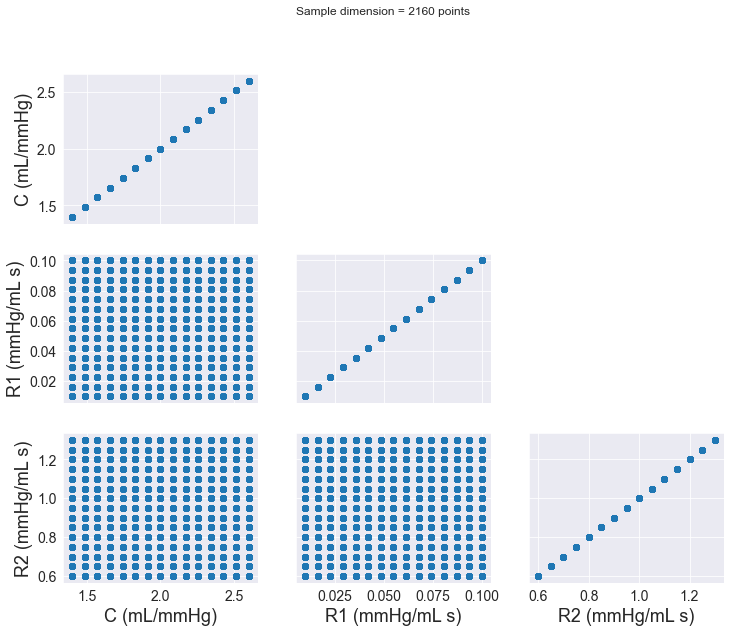
\includegraphics[width=1\textwidth]{images/Training (risultati)/database.png}
    \caption{Distribution of data in the database.}
    \label{distribuzioneDataset}
\end{figure}

\newpage
\section{Training results}


%******************************
%*********** MAP **************
%******************************
\subsection{Mean arterial pressure (MAP)}
$\text{lr}=0.1$ is set and the early stopper \textit{GLEarlyStoppingCriterion} is used with parameters: $\alpha = 5$, $\text{patience}=2$.


% **********
% MAP - loss
% **********
\subsubsection{Training and validation loss}
The training needed fifty-two EPOCHS (each EPOCH consists of evaluating the gradient on each dataset element), concluded with $\text{R2Score}=0.9999$, $\text{MeanSquaredError}=0.0001$. Figure \ref{MAP - loss} shows the training and validation loss trend with MSE and R2Score; early stopper trend in green.
\begin{figure}[h]
    \centering
    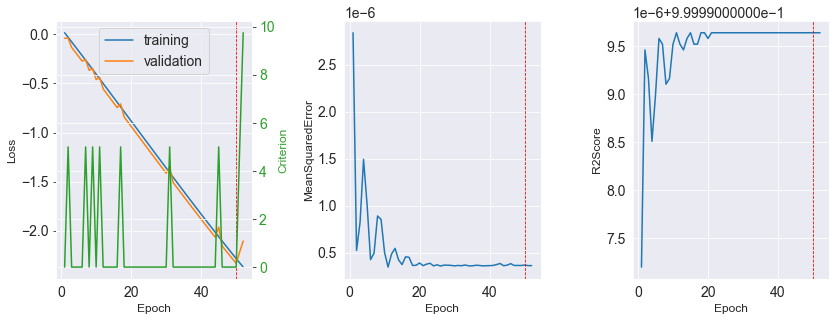
\includegraphics[width=1\textwidth]{images/Training (risultati)/MAP/MAP - loss.png}
    \caption{MAP: progress of training and validation loss, early stopper, R2Score e MSE.}
    \label{MAP - loss}
\end{figure}

\newpage



% **********
% MAP - inference
% **********
\subsubsection{Approximation of input data}
Figure \ref{MAP - inference} shows how the predictions approximate the input data. The length of the error bars is $0.0015$, so they are very short indicating high accuracy.

\begin{figure}[!htb]
    \centering
    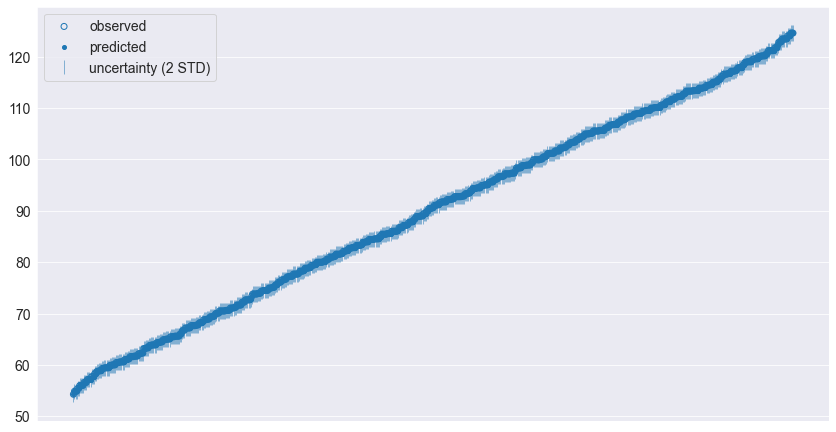
\includegraphics[width=1\textwidth]{images/Training (risultati)/MAP/MAP - inference.png}
    \caption{MAP: predictions about the input data.}
    \label{MAP - inference}
\end{figure}



% **********
% MAP - C
% **********
\subsubsection{Dependence on $C$}
To study the dependence of MAP on $C$, ninety equidistant $C$ values are taken in the same range used for creating the input database and, fixed the values of $R_1$ and $R_2$ to those found in their approximation in \ref{stimaCR}, a file of $C$, $R_1$ and $R_2$ combinations is generated. For each combination, the pressure approximation with the Windkessel model is found and MAP calculated; with the combination of compliance and strengths, MAP is then estimated using the model already trained. The same is then done on two intervals adjacent to the training interval and broaden the $10\%$ of the training interval. The overall result is shown in figure \ref{MAP - C - full}, the result in the training interval alone in \ref{MAP - C - training}, the result in the individual adjacent intervals in \ref{MAP - C - sx} and \ref{MAP - C - dx}.

\begin{figure}
    \centering
    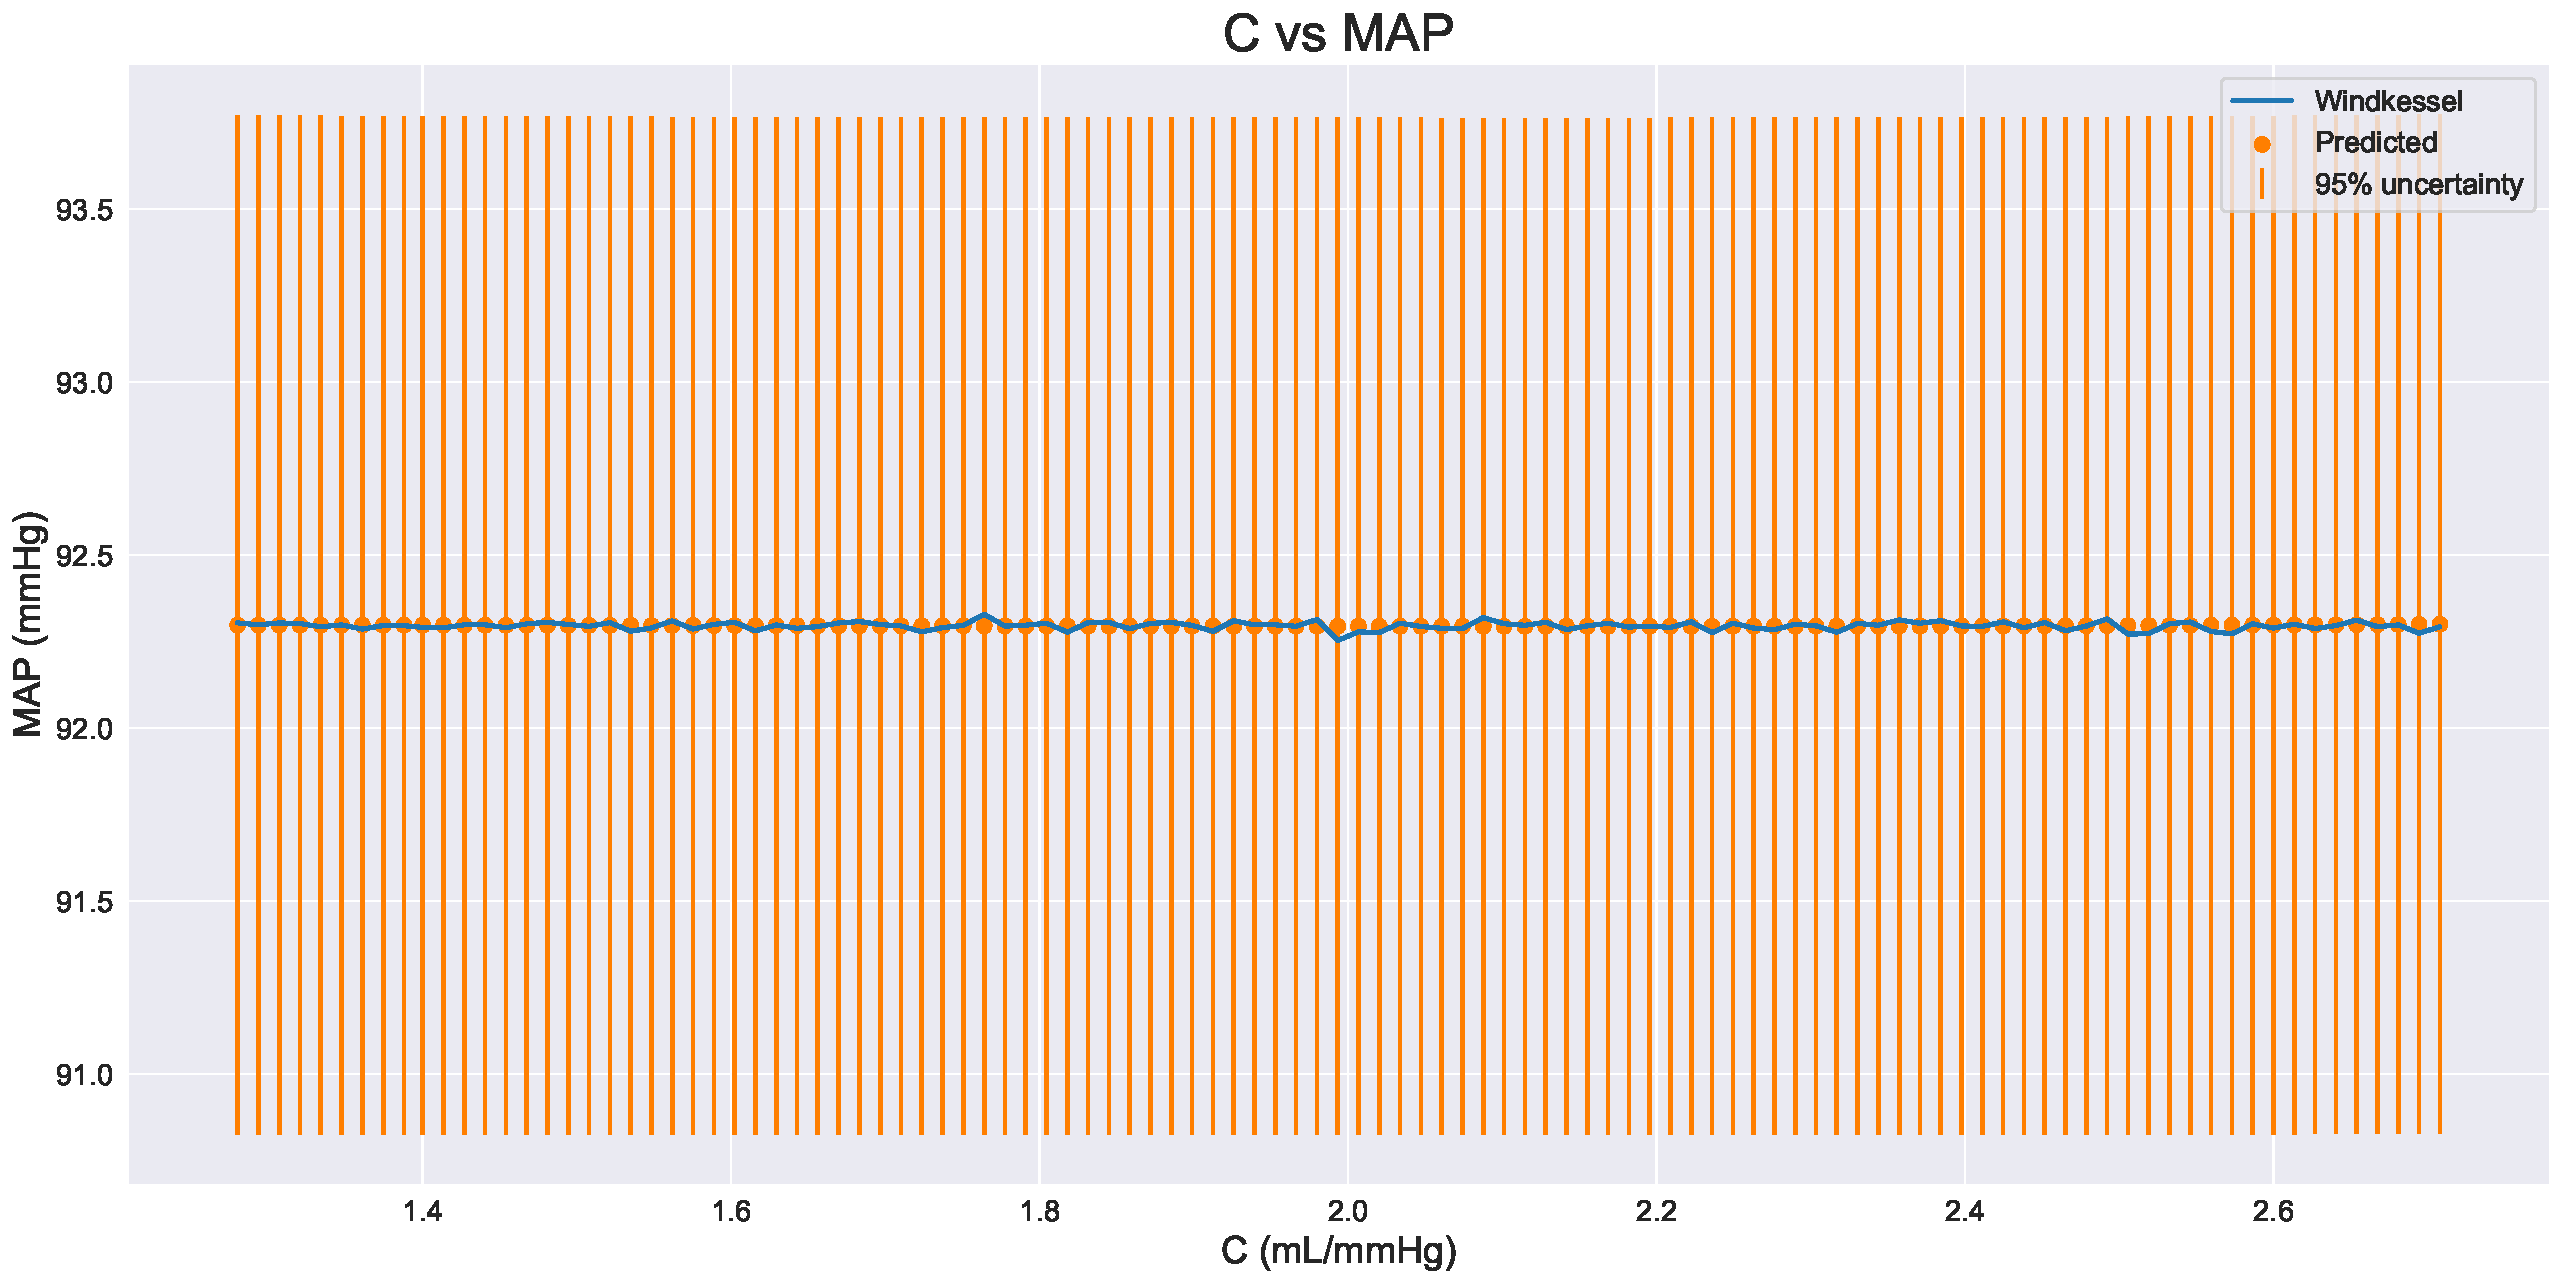
\includegraphics[width=1\textwidth]{images/Training (risultati)/MAP/MAP - C - full.pdf}
    \caption{Dependence of MAP on $C$ on the training interval and two adjacent intervals.}
    \label{MAP - C - full}
\end{figure}


\begin{figure}
    \centering
    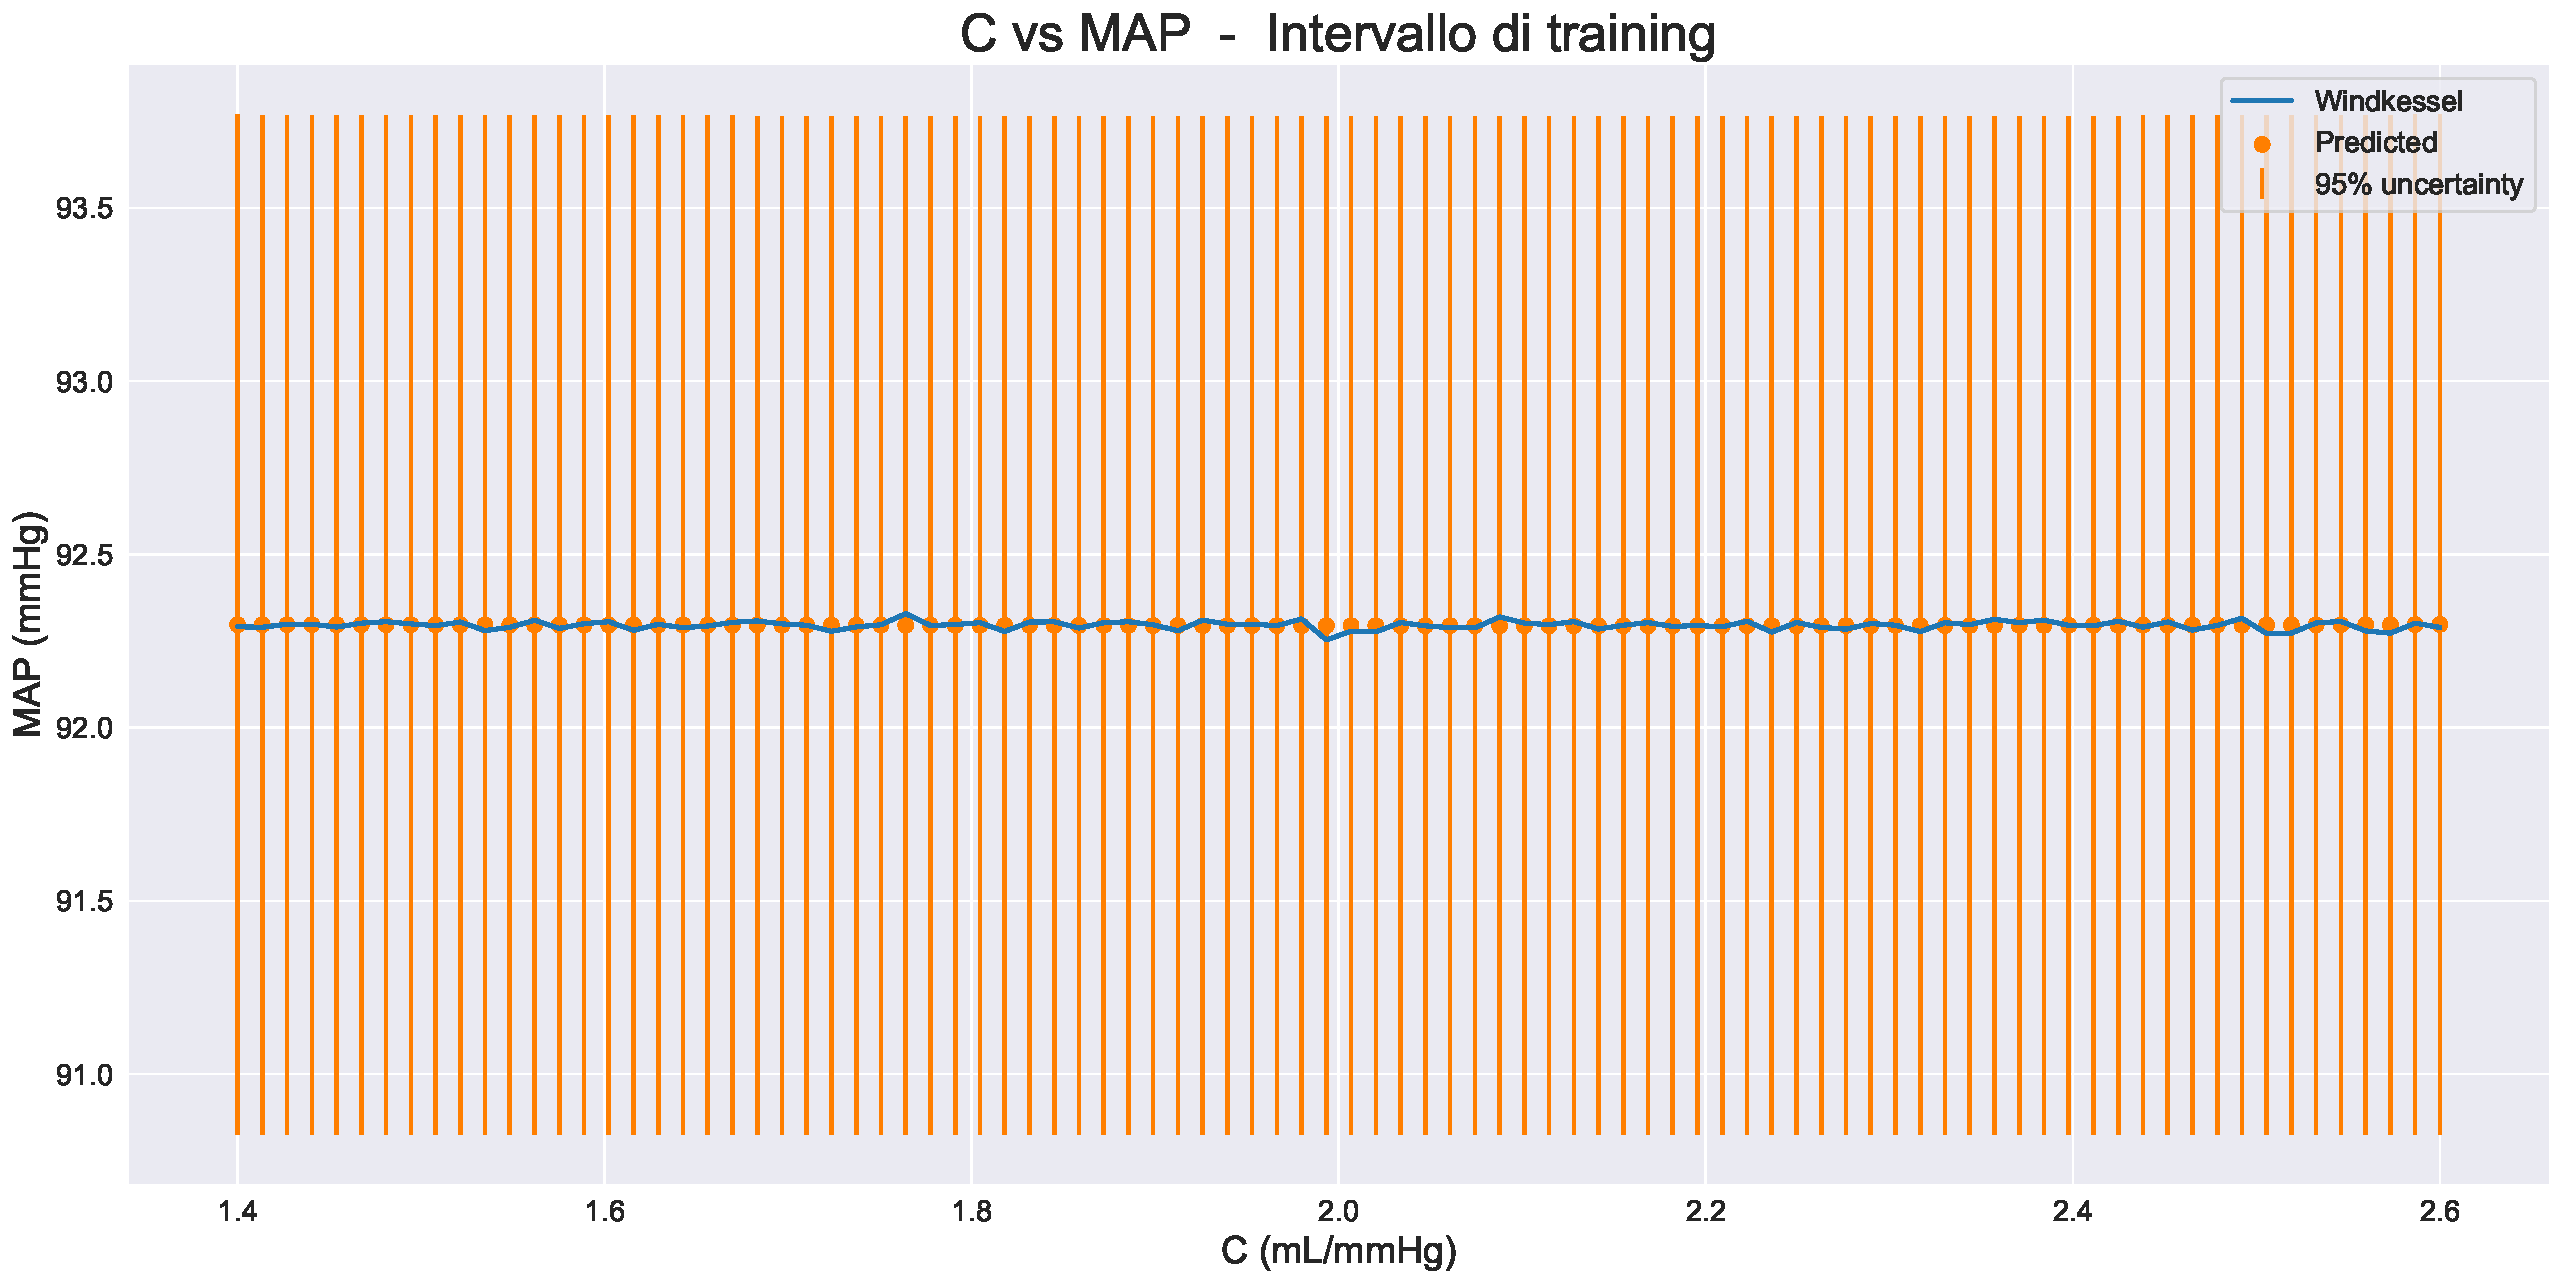
\includegraphics[width=1\textwidth]{images/Training (risultati)/MAP/MAP - C - training.pdf}
    \caption{Dependence of MAP on $C$ over the training interval.}
    \label{MAP - C - training}
\end{figure}


\begin{figure}
    \centering
    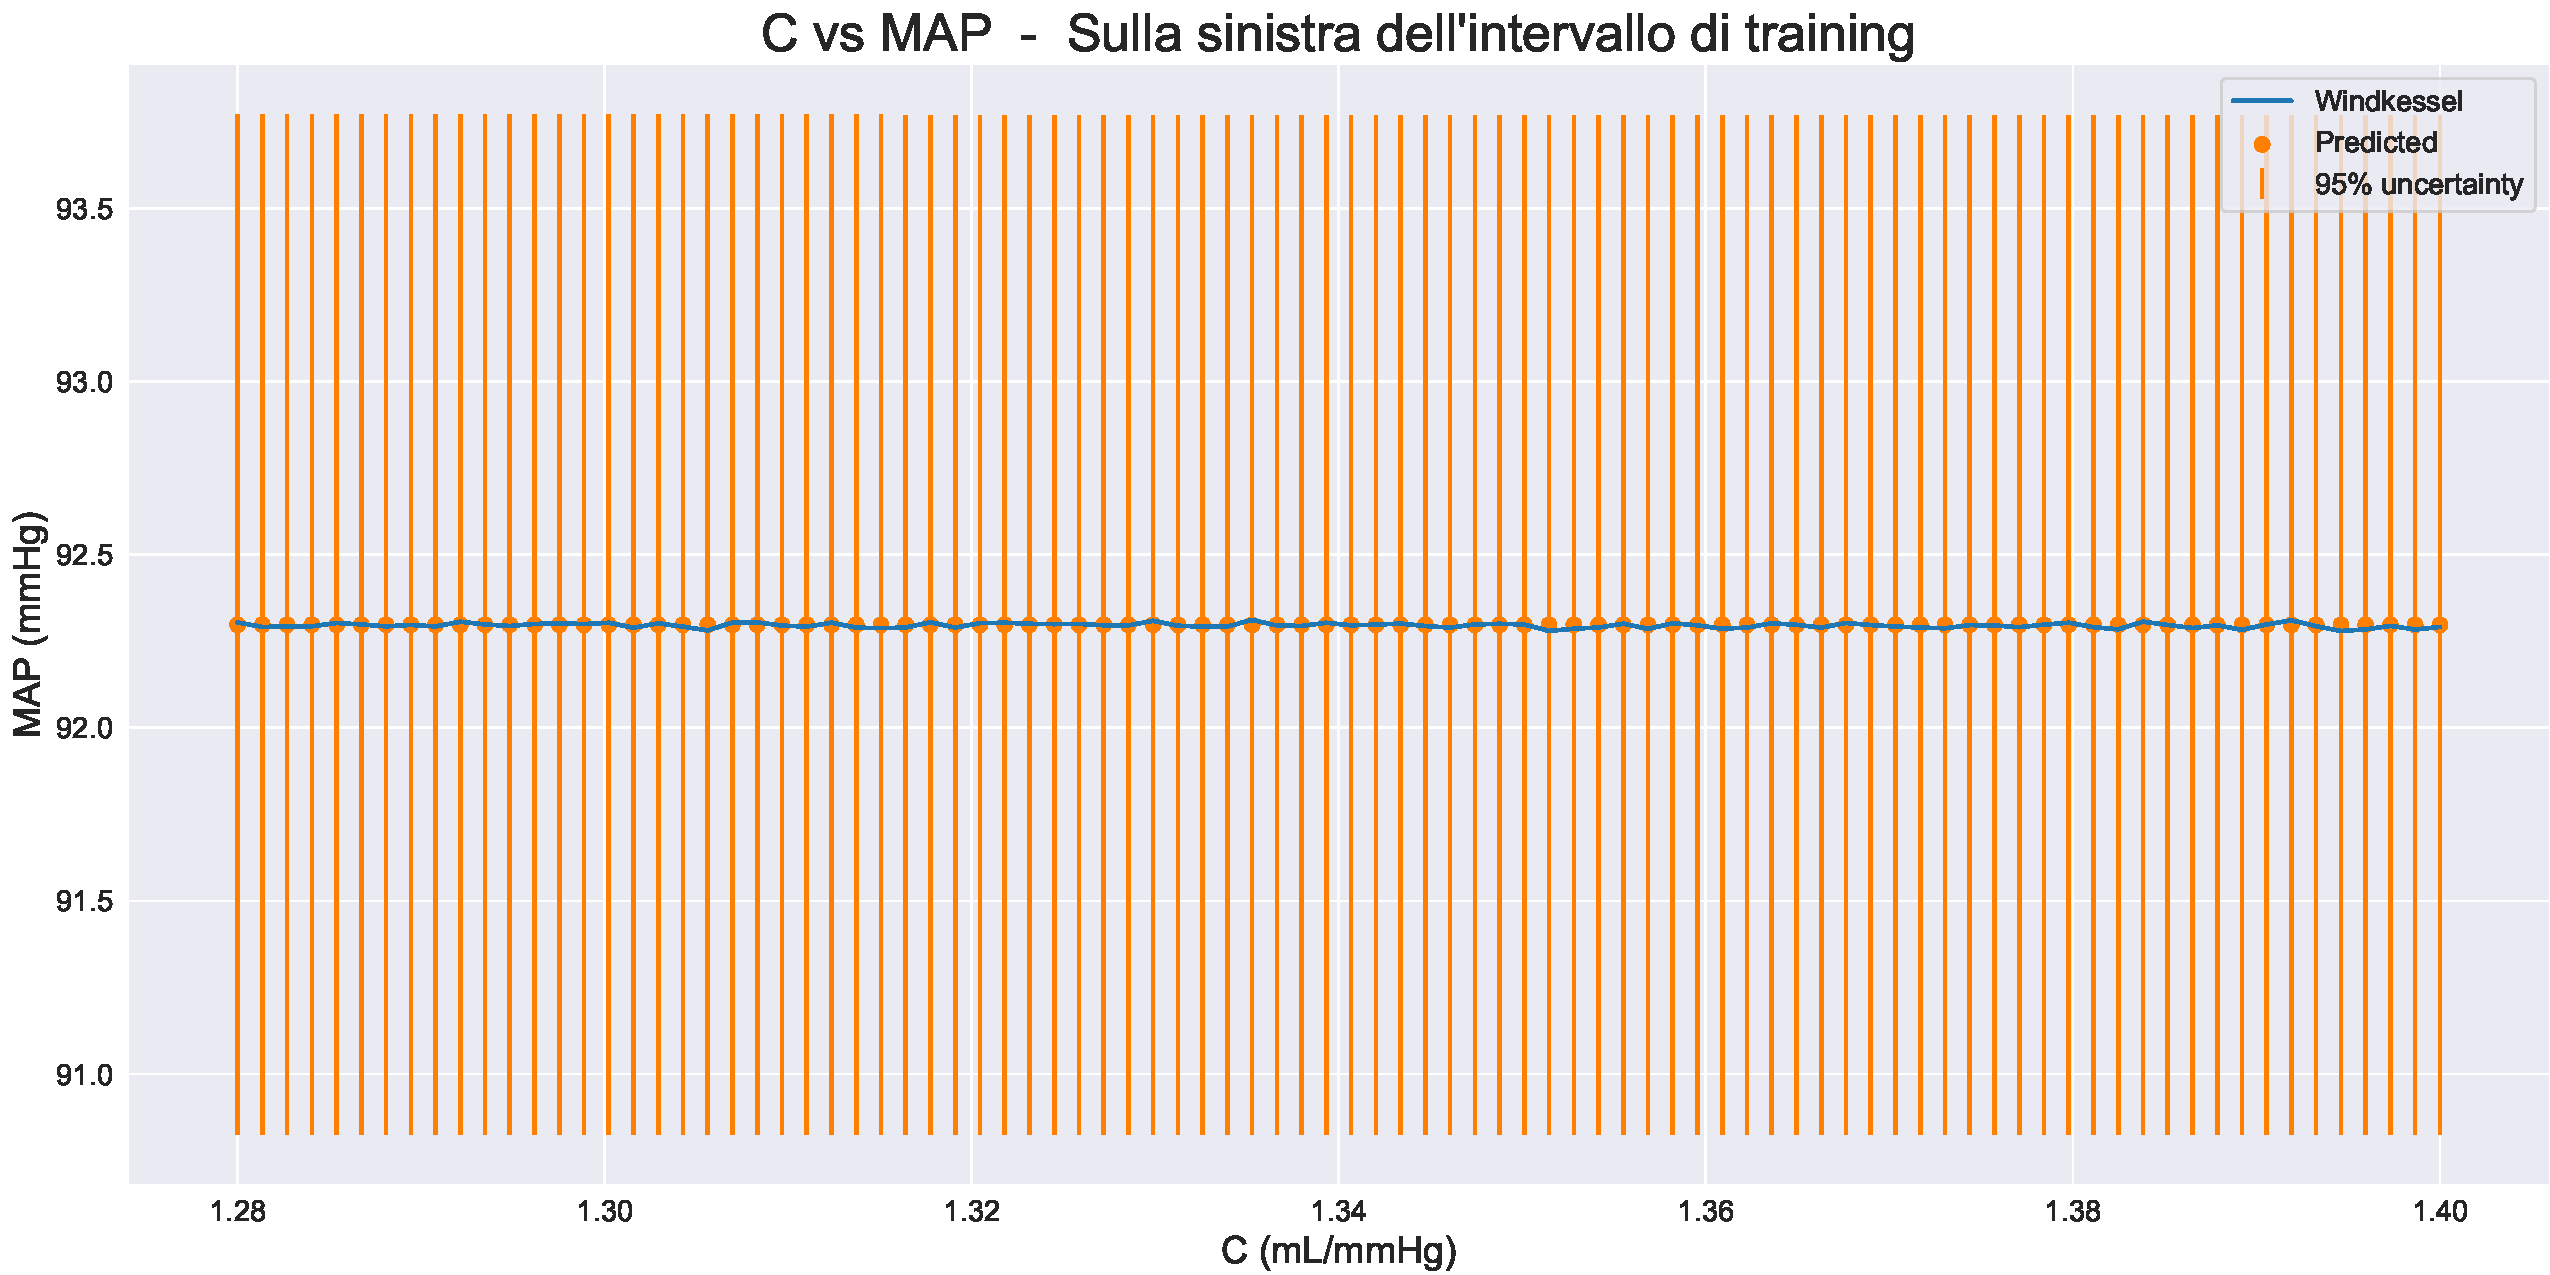
\includegraphics[width=1\textwidth]{images/Training (risultati)/MAP/MAP - C - sx.pdf}
    \caption{Dependence of MAP on $C$ on the adjacent interval to the left of the training interval.}
    \label{MAP - C - sx}
\end{figure}



\begin{figure}
    \centering
    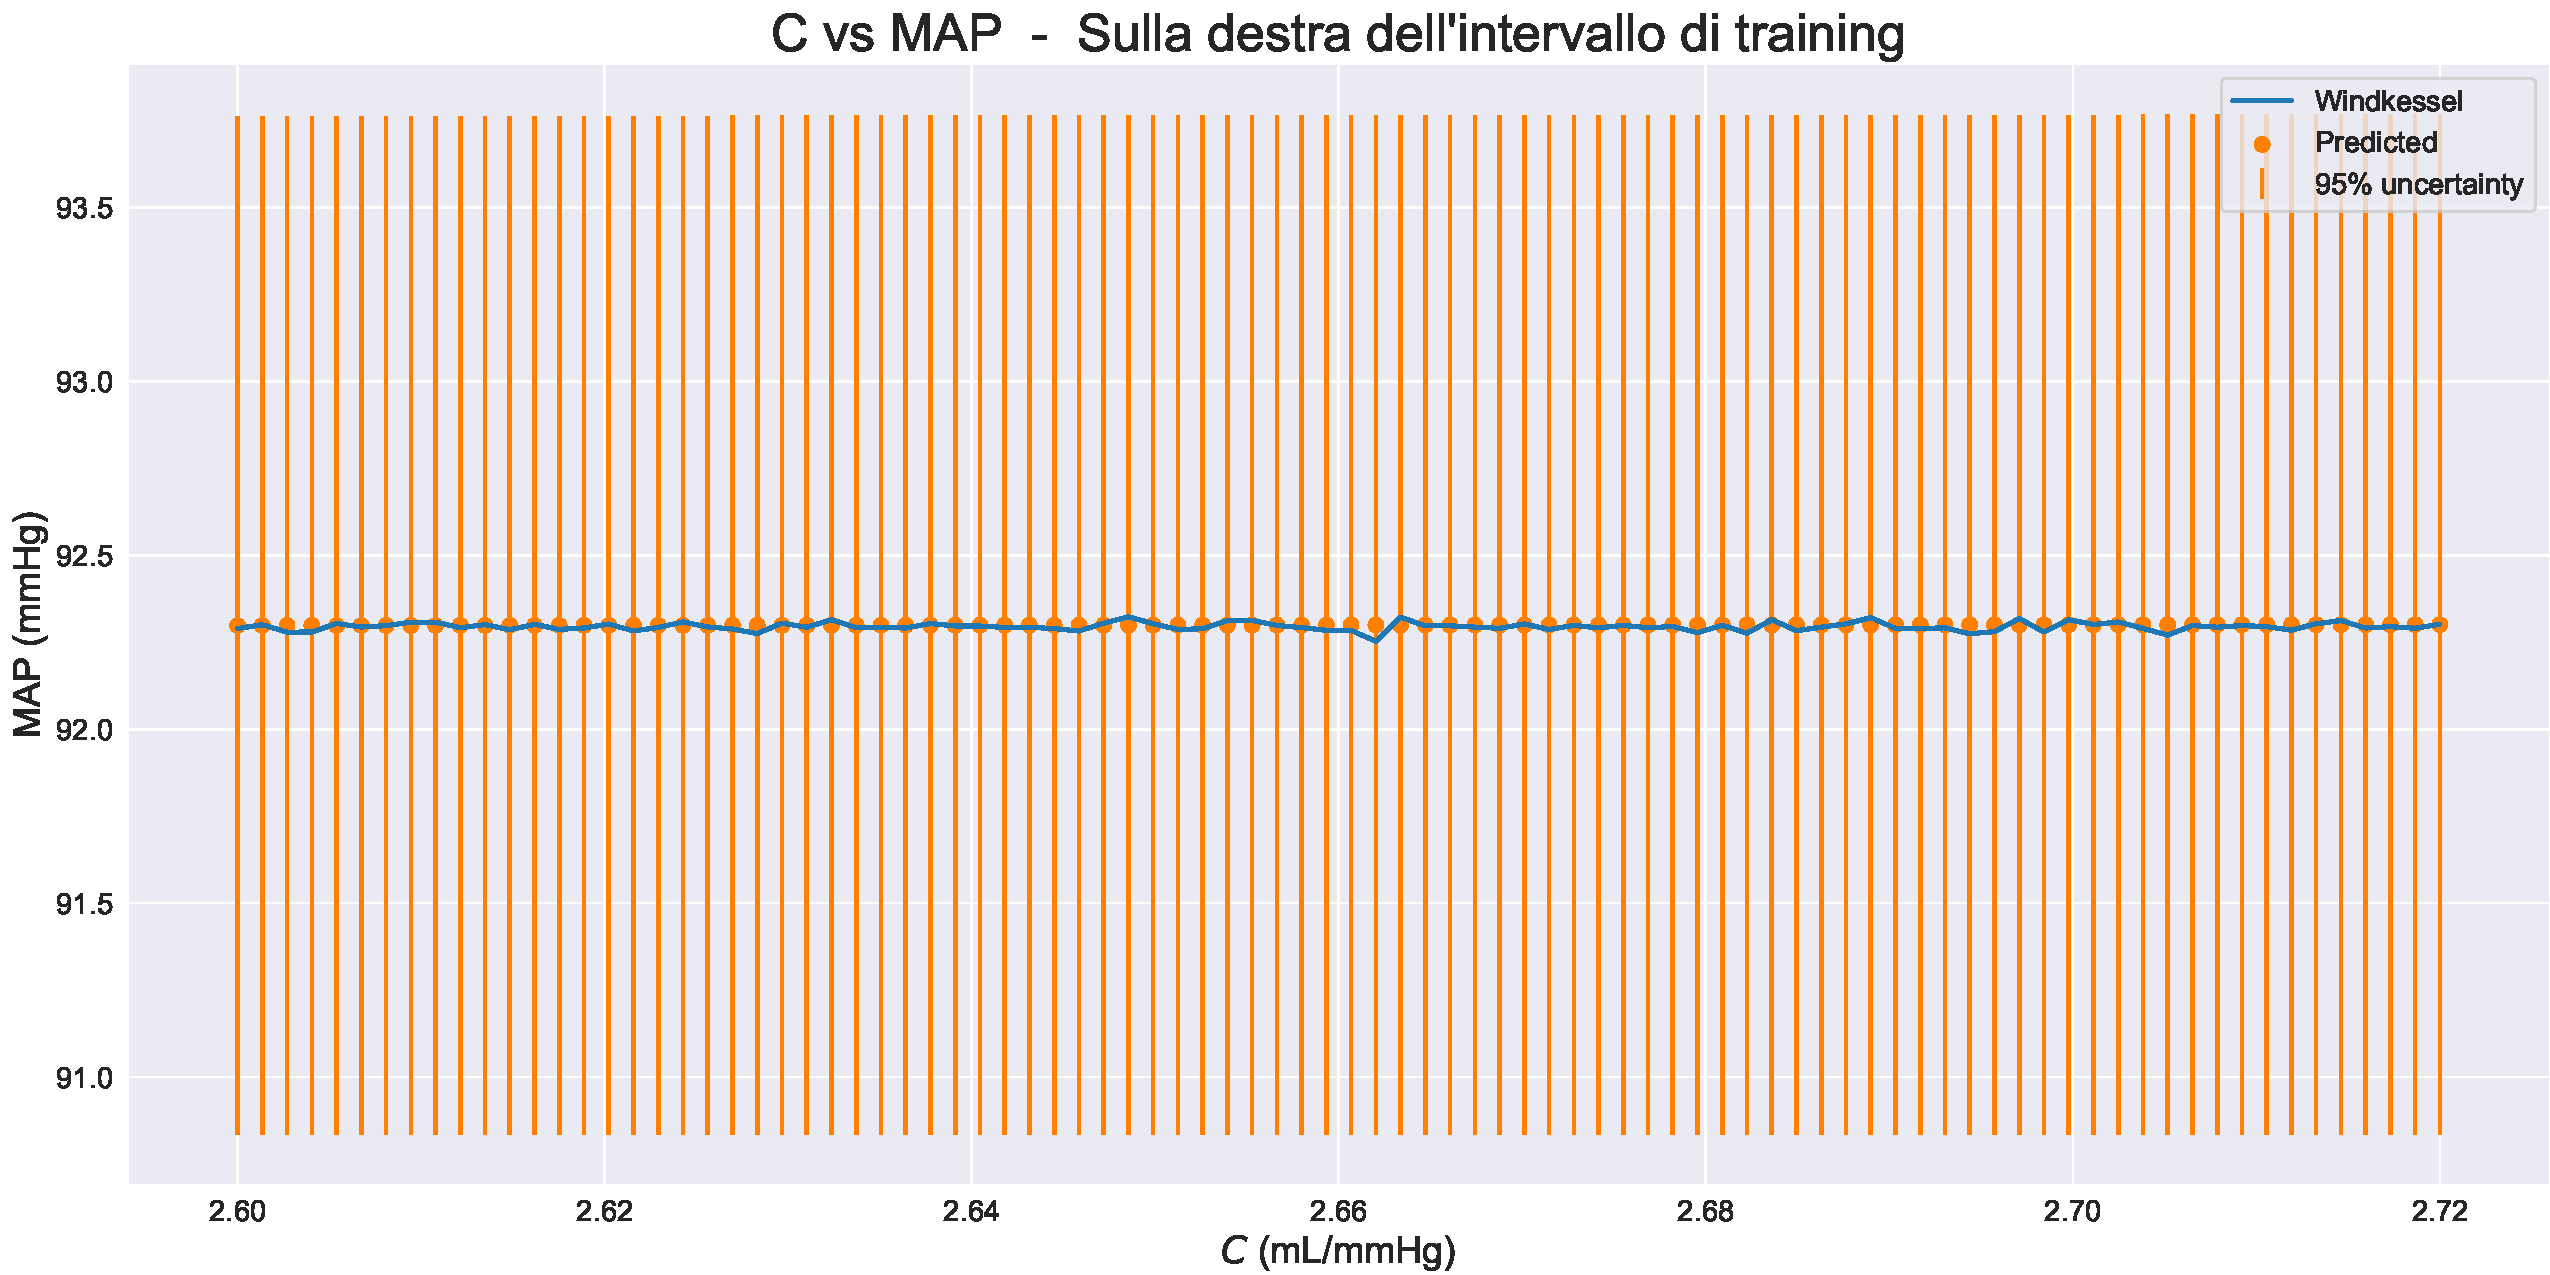
\includegraphics[width=1\textwidth]{images/Training (risultati)/MAP/MAP - C - dx.pdf}
    \caption{Dependence of MAP on $C$ on the adjacent interval to the right of the training interval.}
    \label{MAP - C - dx}
\end{figure}




\newpage
% **********
% MAP - R1
% **********
\subsubsection{Dependence on $R_1$}
The same approach is used to study the dependence on $R_1$. The overall result is shown in figure \ref{MAP - R1 - full}, the result in the training interval alone in \ref{MAP - R1 - training}, the result in the individual adjoint intervals in \ref{MAP - R1 - sx} and \ref{MAP - R1 - dx}.

\begin{figure}[!htb]
    \centering
    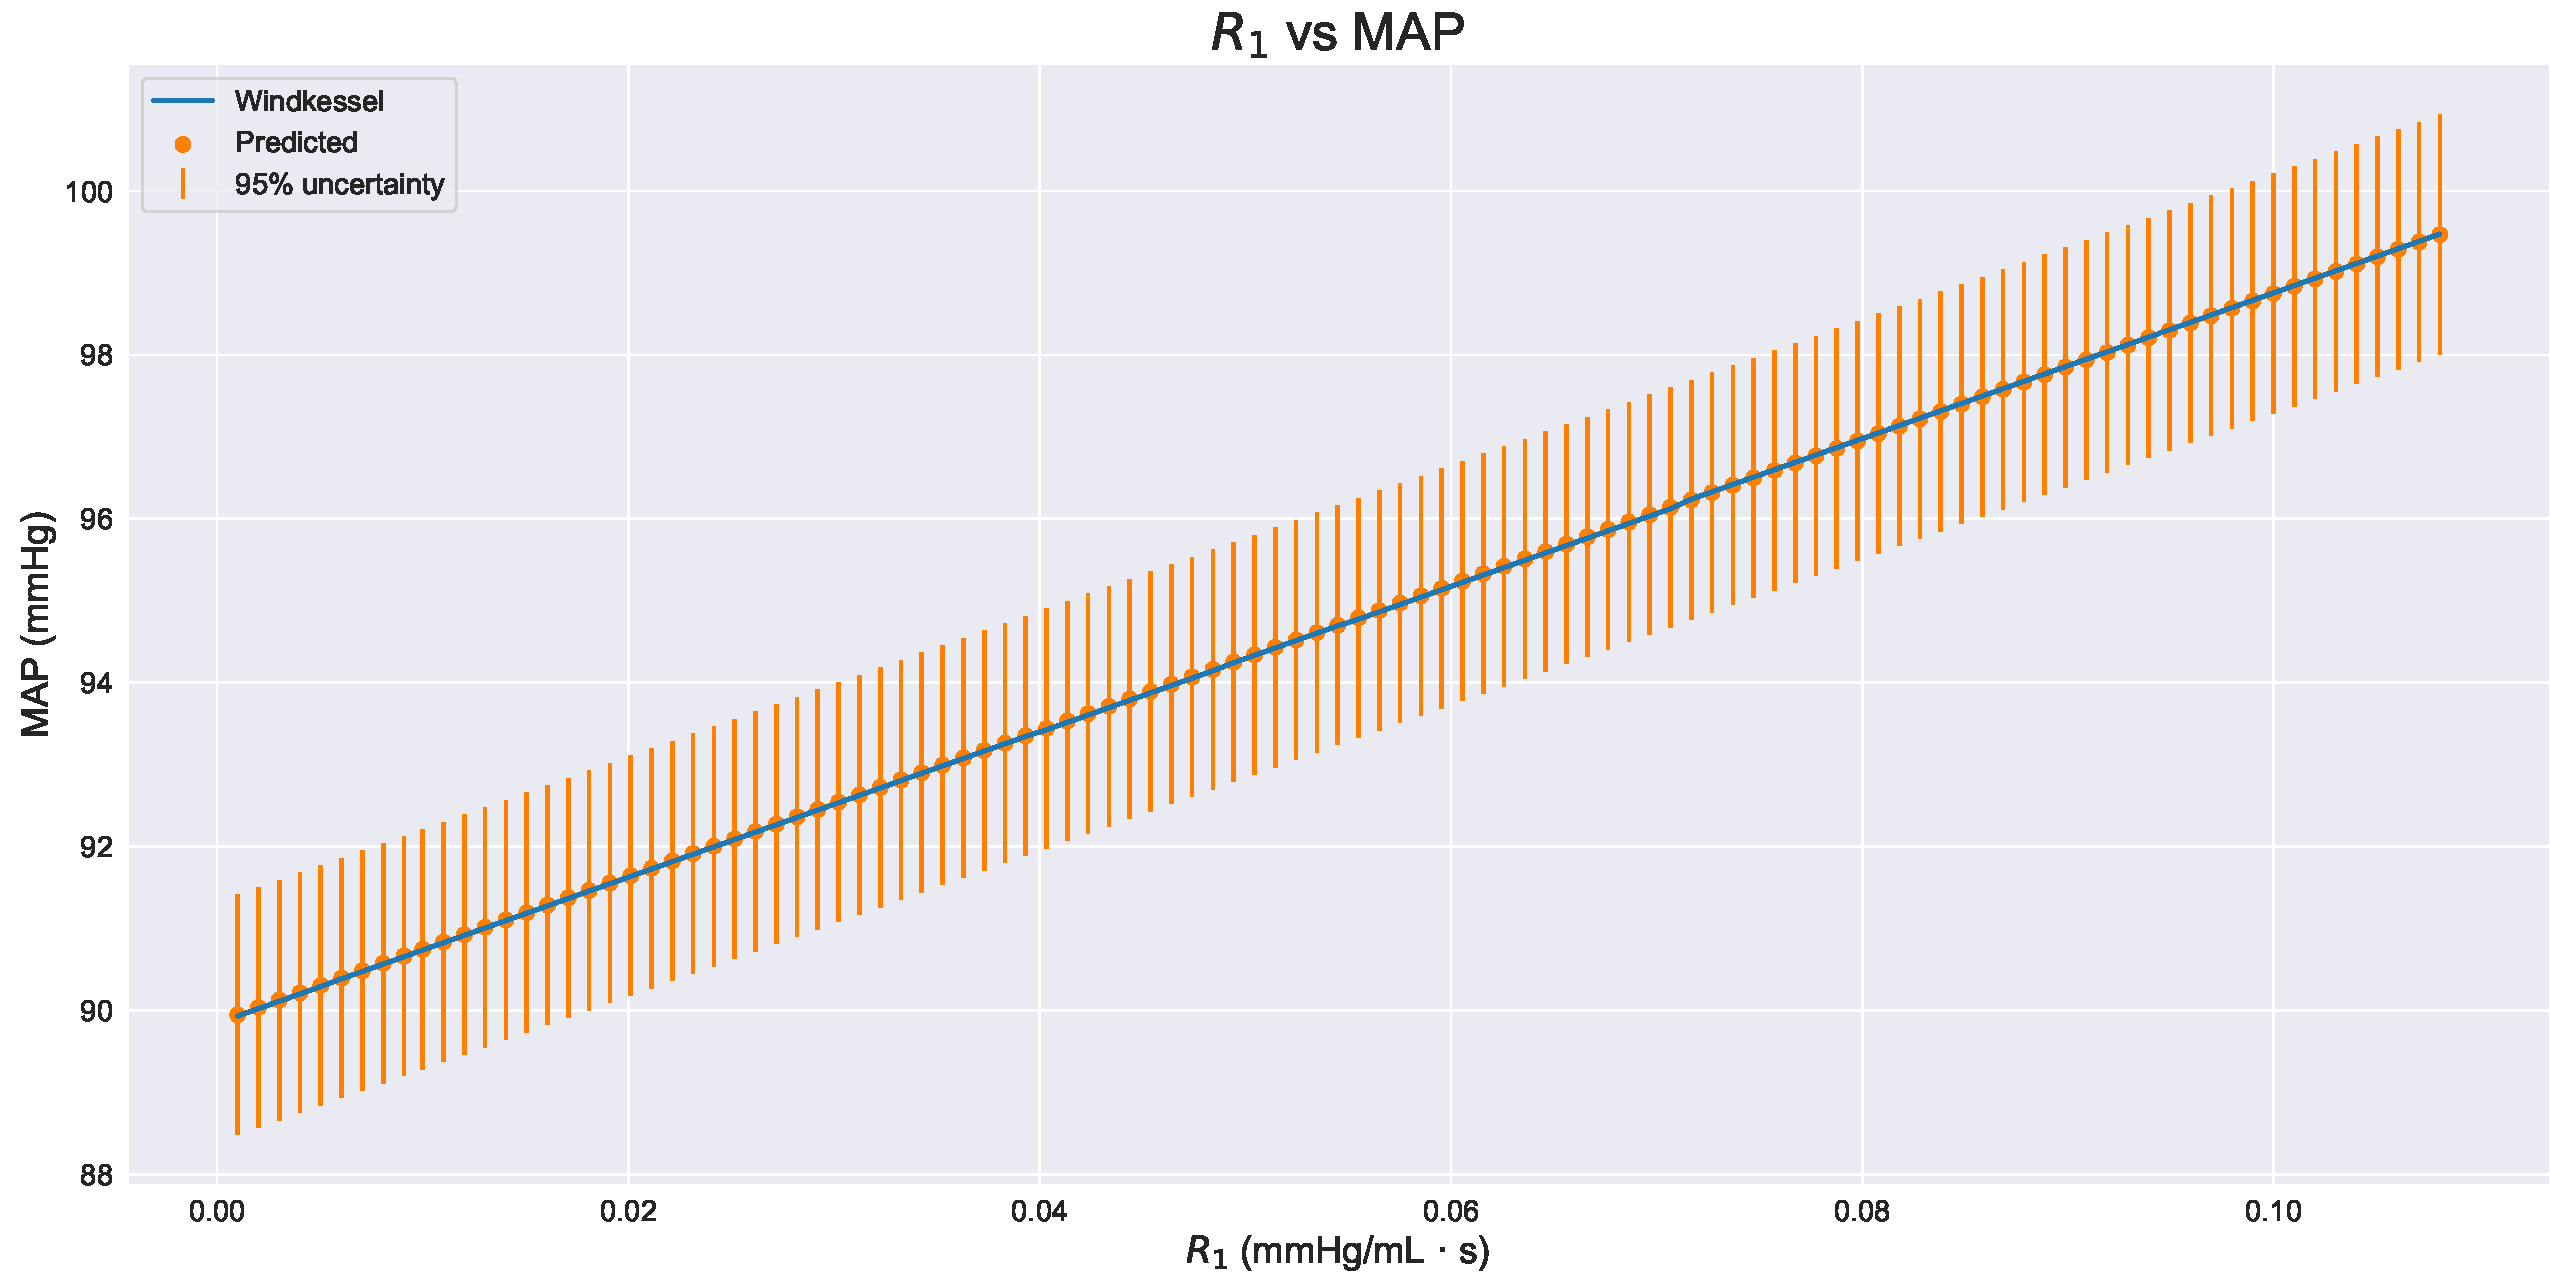
\includegraphics[width=1\textwidth]{images/Training (risultati)/MAP/MAP - R1 - full.pdf}
    \caption{Dependence of MAP on $R1$ on the training interval and two adjacent intervals.}
    \label{MAP - R1 - full}
\end{figure}

\vspace{1cm}

\begin{figure}[!htb]
    \centering
    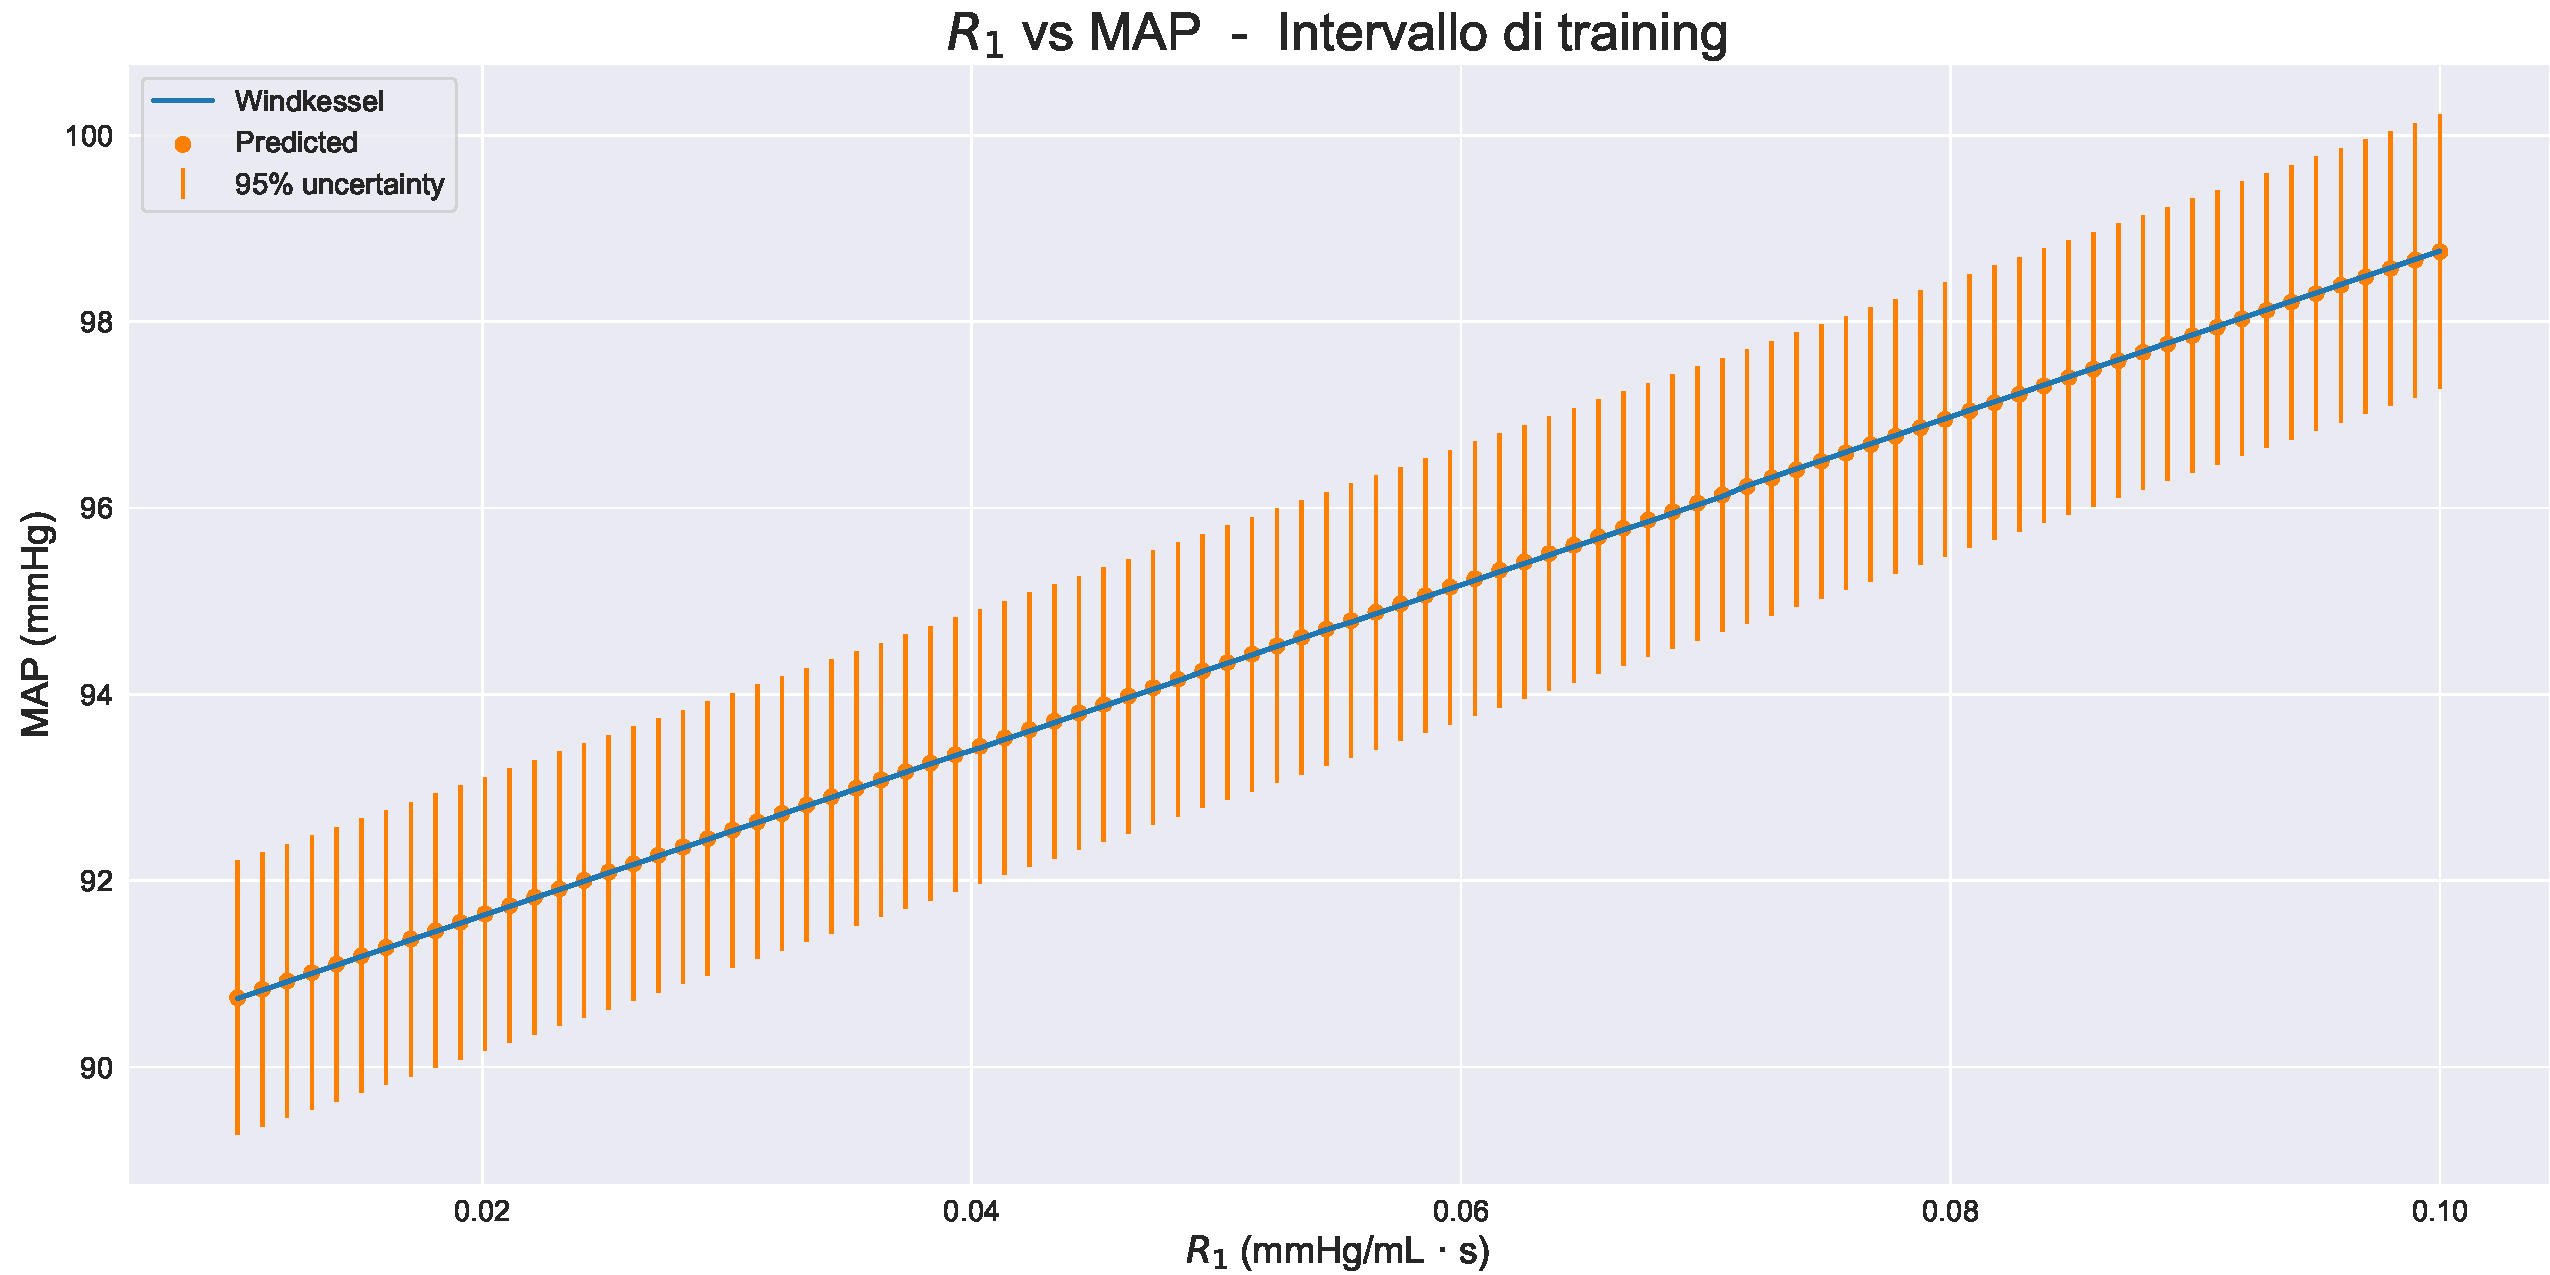
\includegraphics[width=1\textwidth]{images/Training (risultati)/MAP/MAP - R1 - training.pdf}
    \caption{Dependence of MAP on $R1$ over the training interval.}
    \label{MAP - R1 - training}
\end{figure}

\begin{figure}
    \centering
    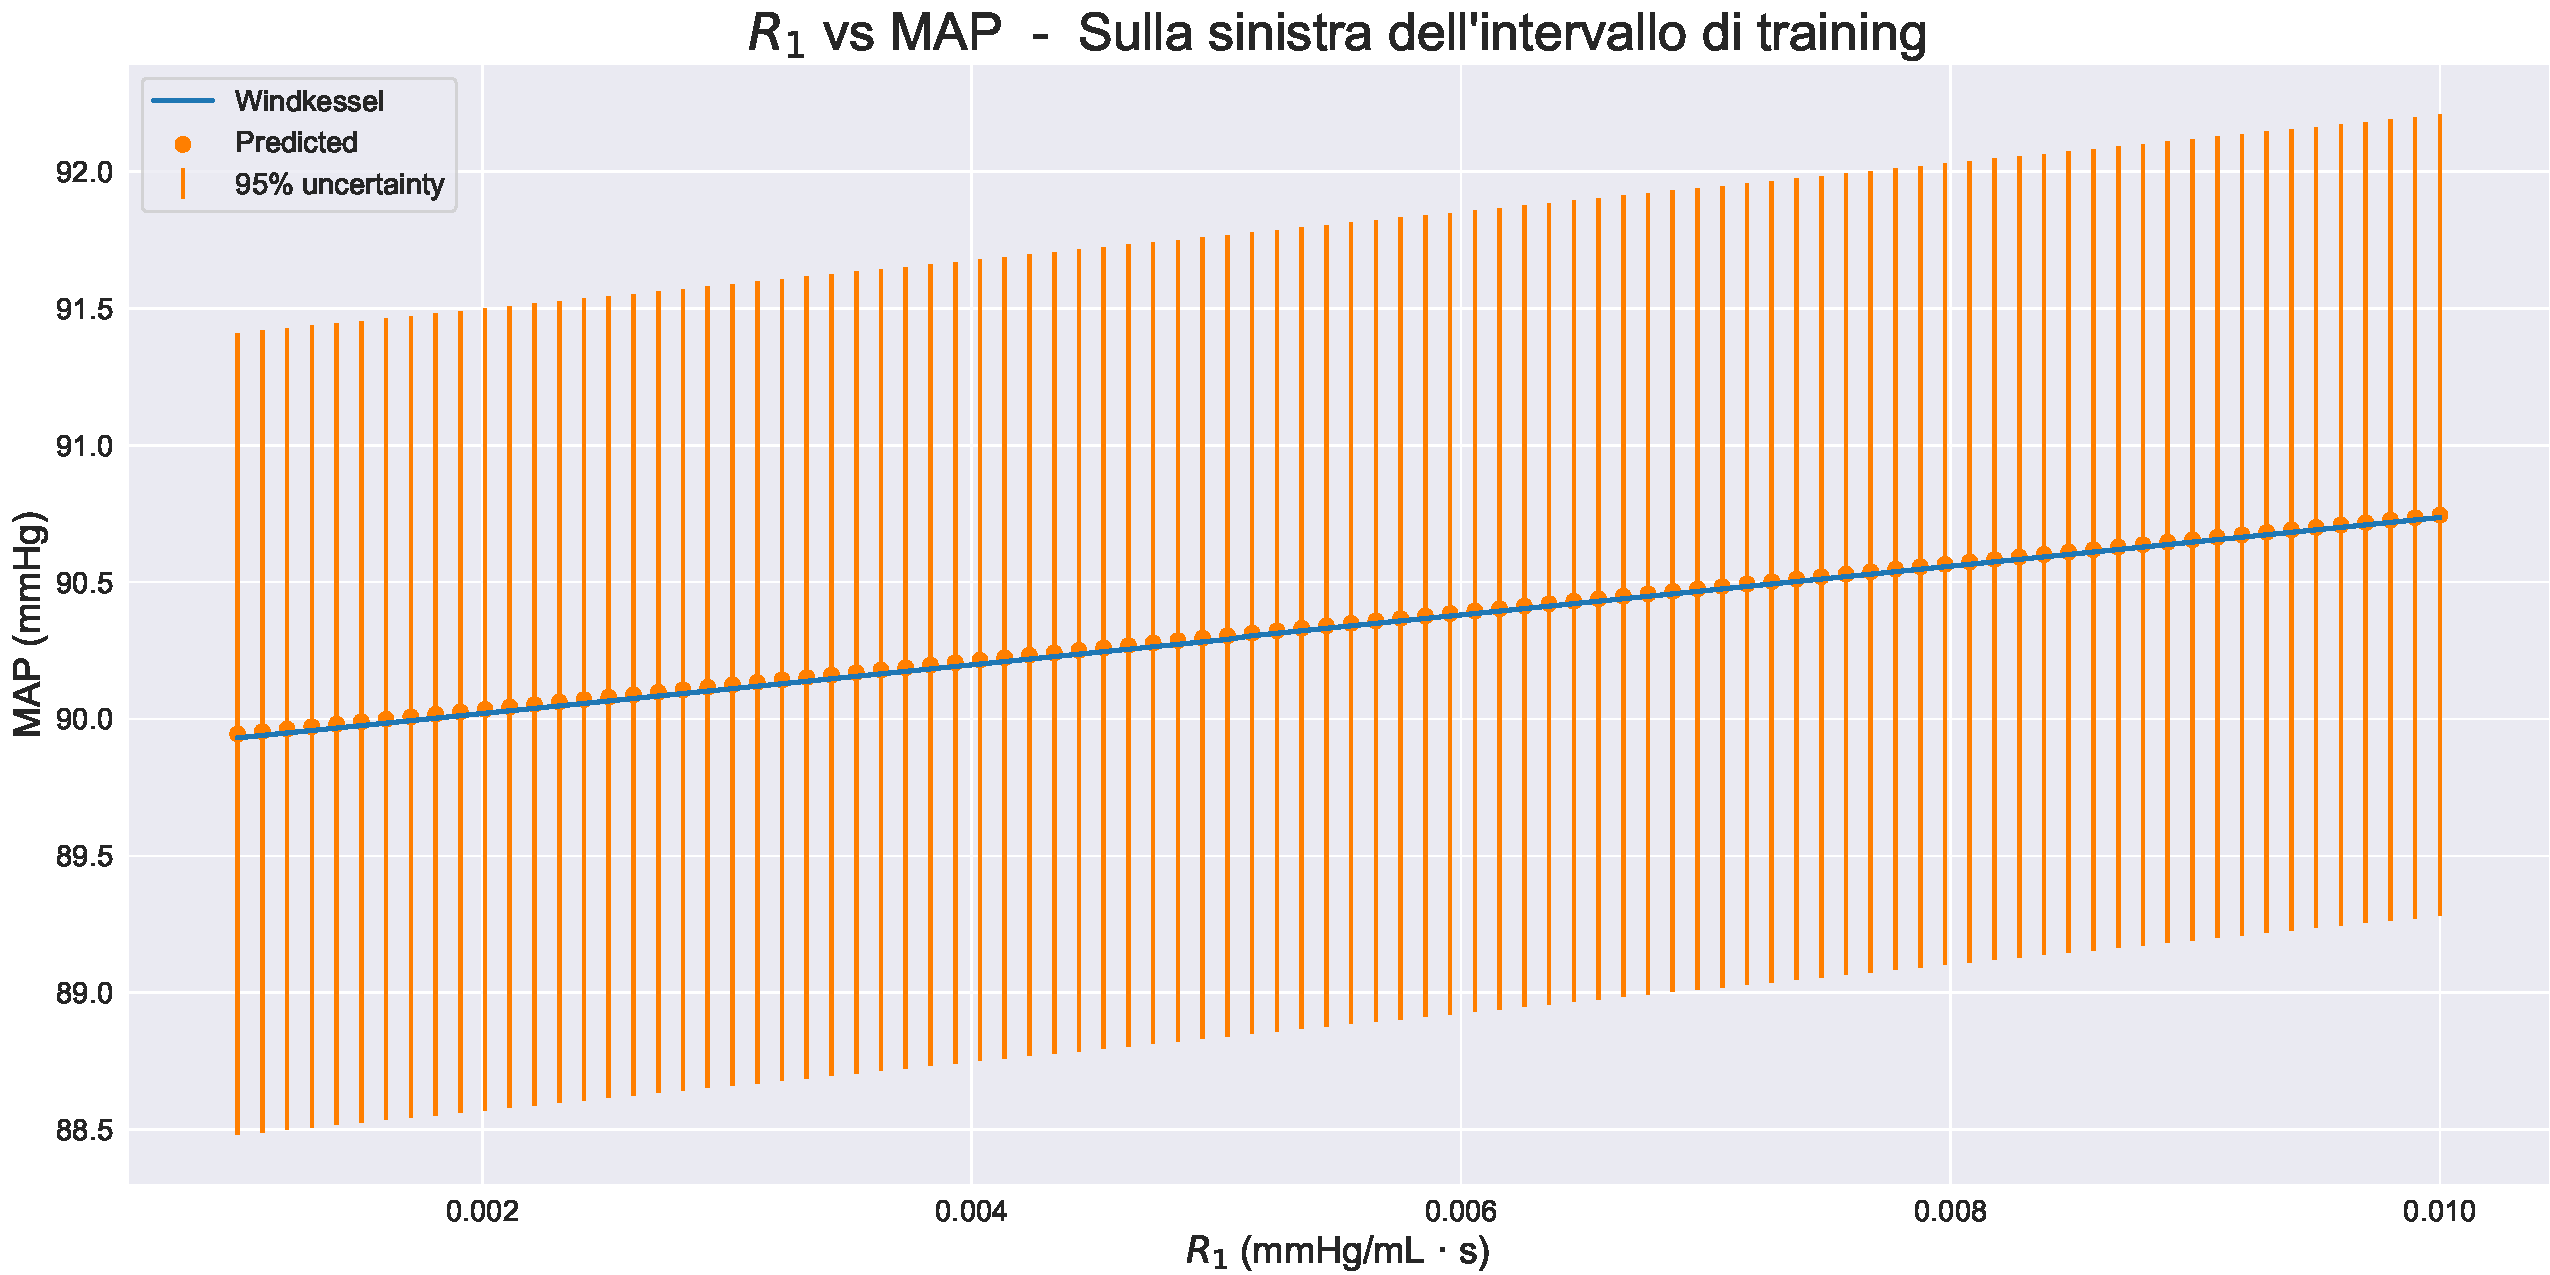
\includegraphics[width=1\textwidth]{images/Training (risultati)/MAP/MAP - R1 - sx.pdf}
    \caption{Dependence of MAP on $R1$ on the adjacent interval to the left of the training interval.}
    \label{MAP - R1 - sx}
\end{figure}


\begin{figure}
    \centering
    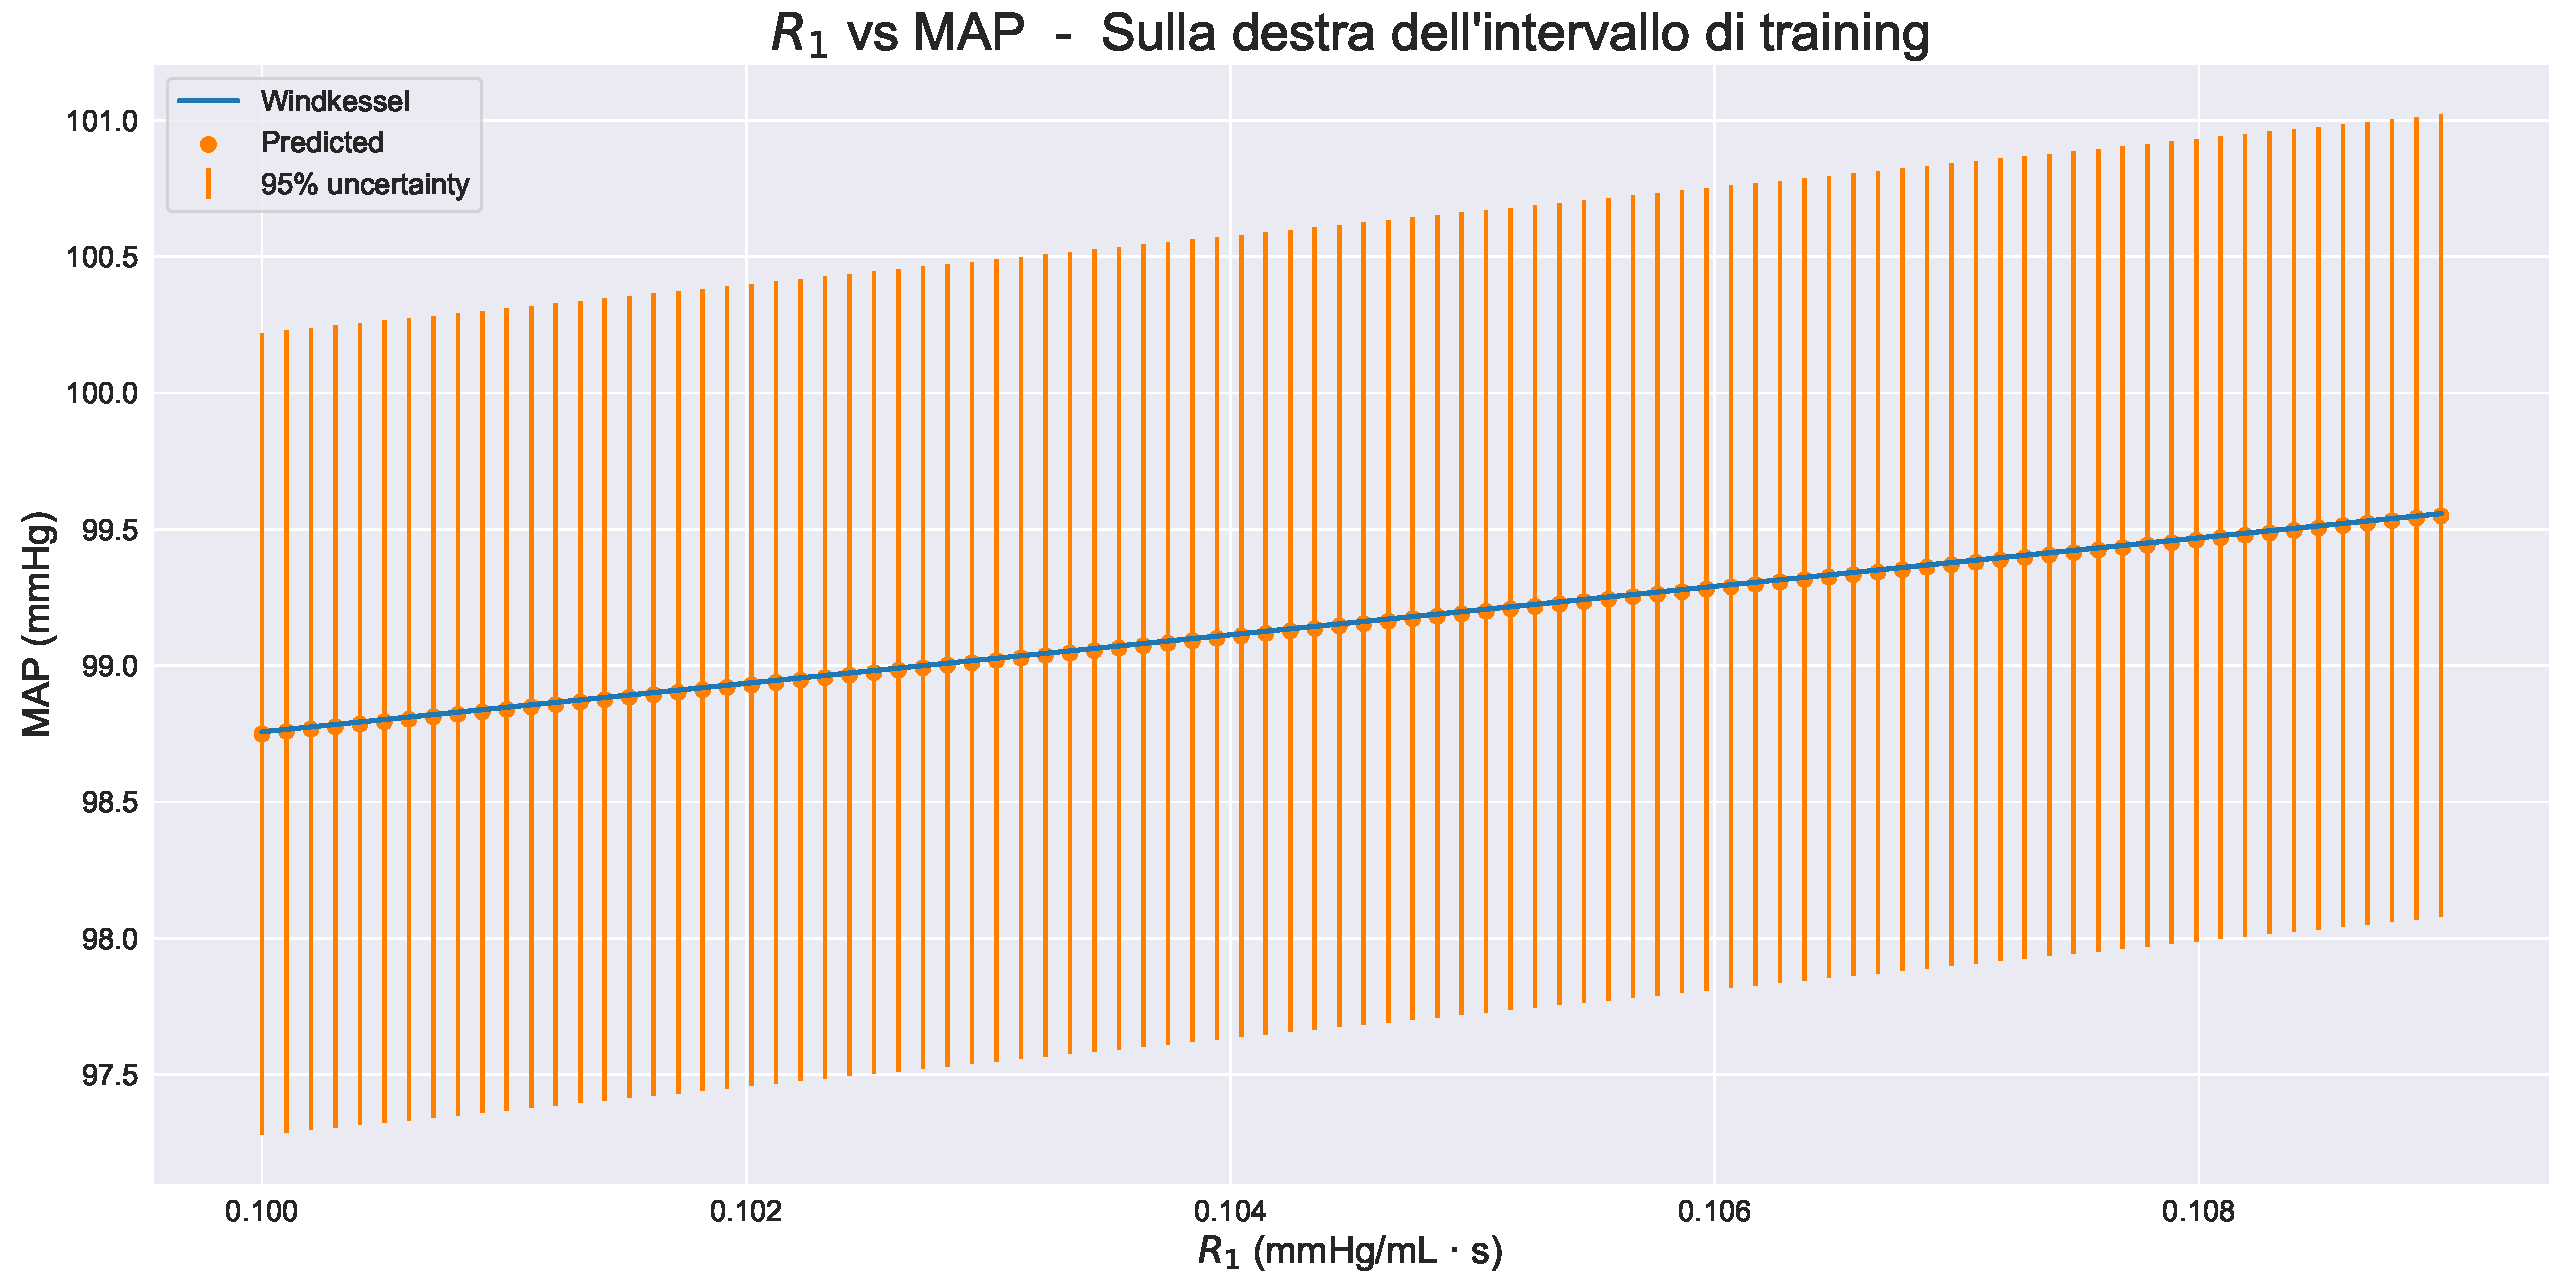
\includegraphics[width=1\textwidth]{images/Training (risultati)/MAP/MAP - R1 - dx.pdf}
    \caption{Dependence of MAP on $R1$ on the adjacent interval to the right of the training interval.}
    \label{MAP - R1 - dx}
\end{figure}




\newpage
% **********
% MAP - R2
% **********
\subsubsection{Dependence on $R_2$}
The same approach is used to study the dependence on $R_2$. The overall result is shown in figure \ref{MAP - R2 - full}, the result in the training interval alone in \ref{MAP - R2 - training}, the result in the individual adjoint intervals in \ref{MAP - R2 - sx} and \ref{MAP - R2 - dx}.

\begin{figure}[!htb]
    \centering
    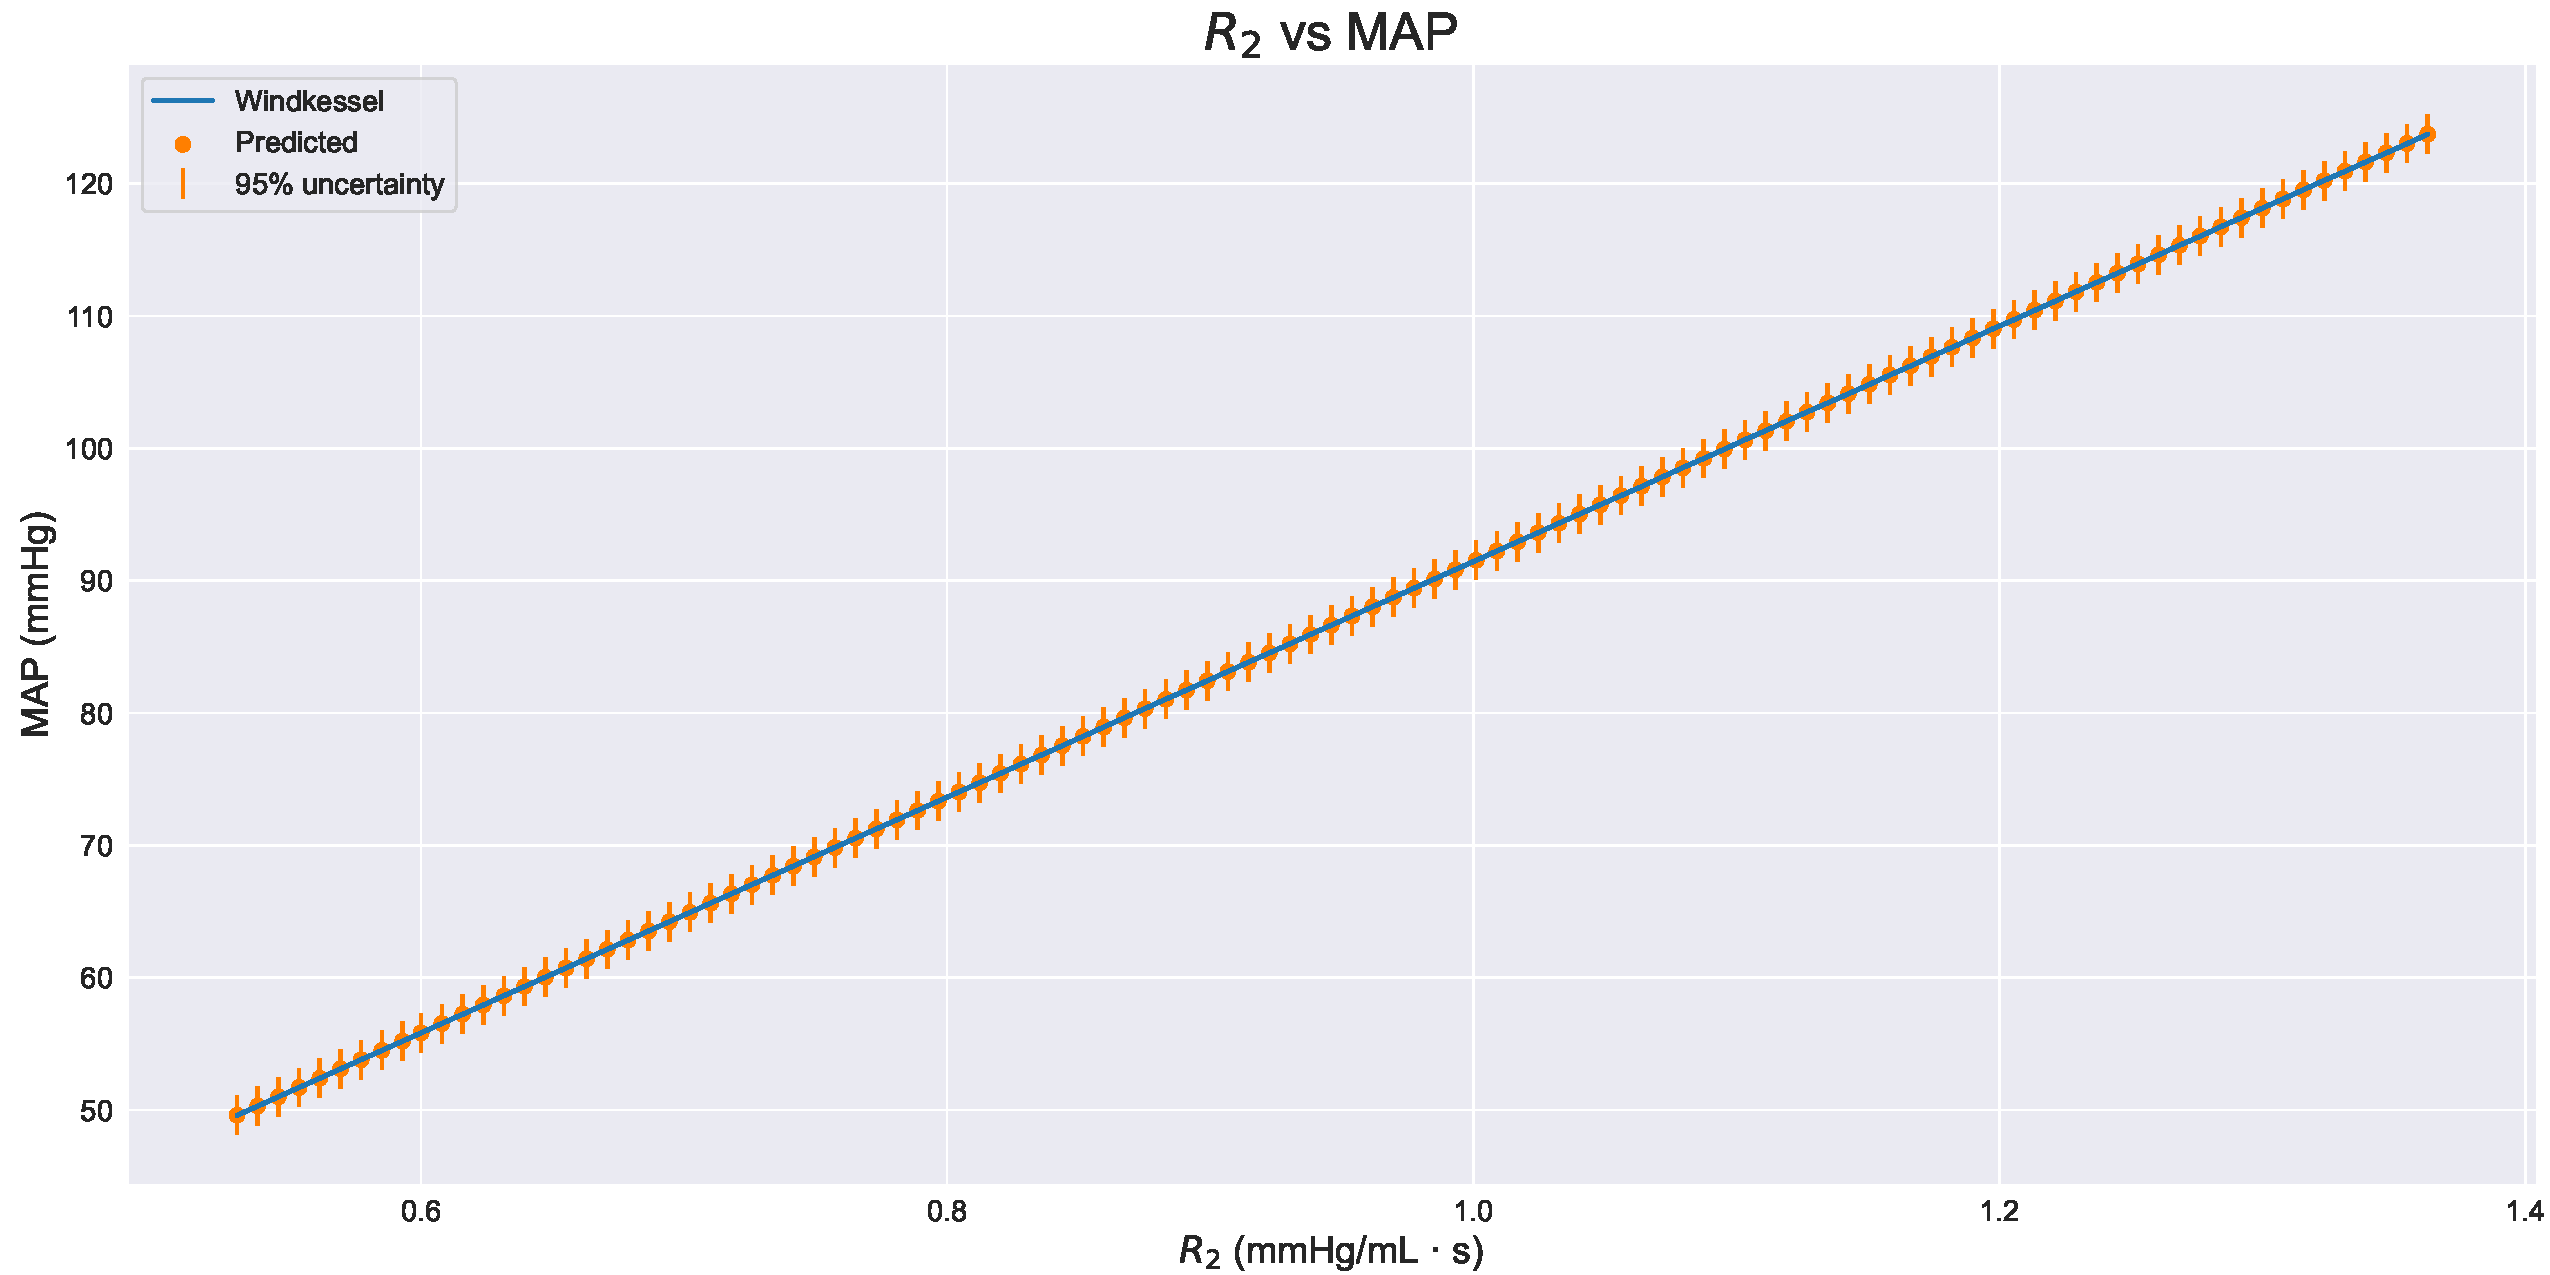
\includegraphics[width=1\textwidth]{images/Training (risultati)/MAP/MAP - R2 - full.pdf}
    \caption{Dependence of MAP on $R2$ over the training interval and two adjacent intervals.}
    \label{MAP - R2 - full}
\end{figure}

\vspace{1cm}

\begin{figure}[!htb]
    \centering
    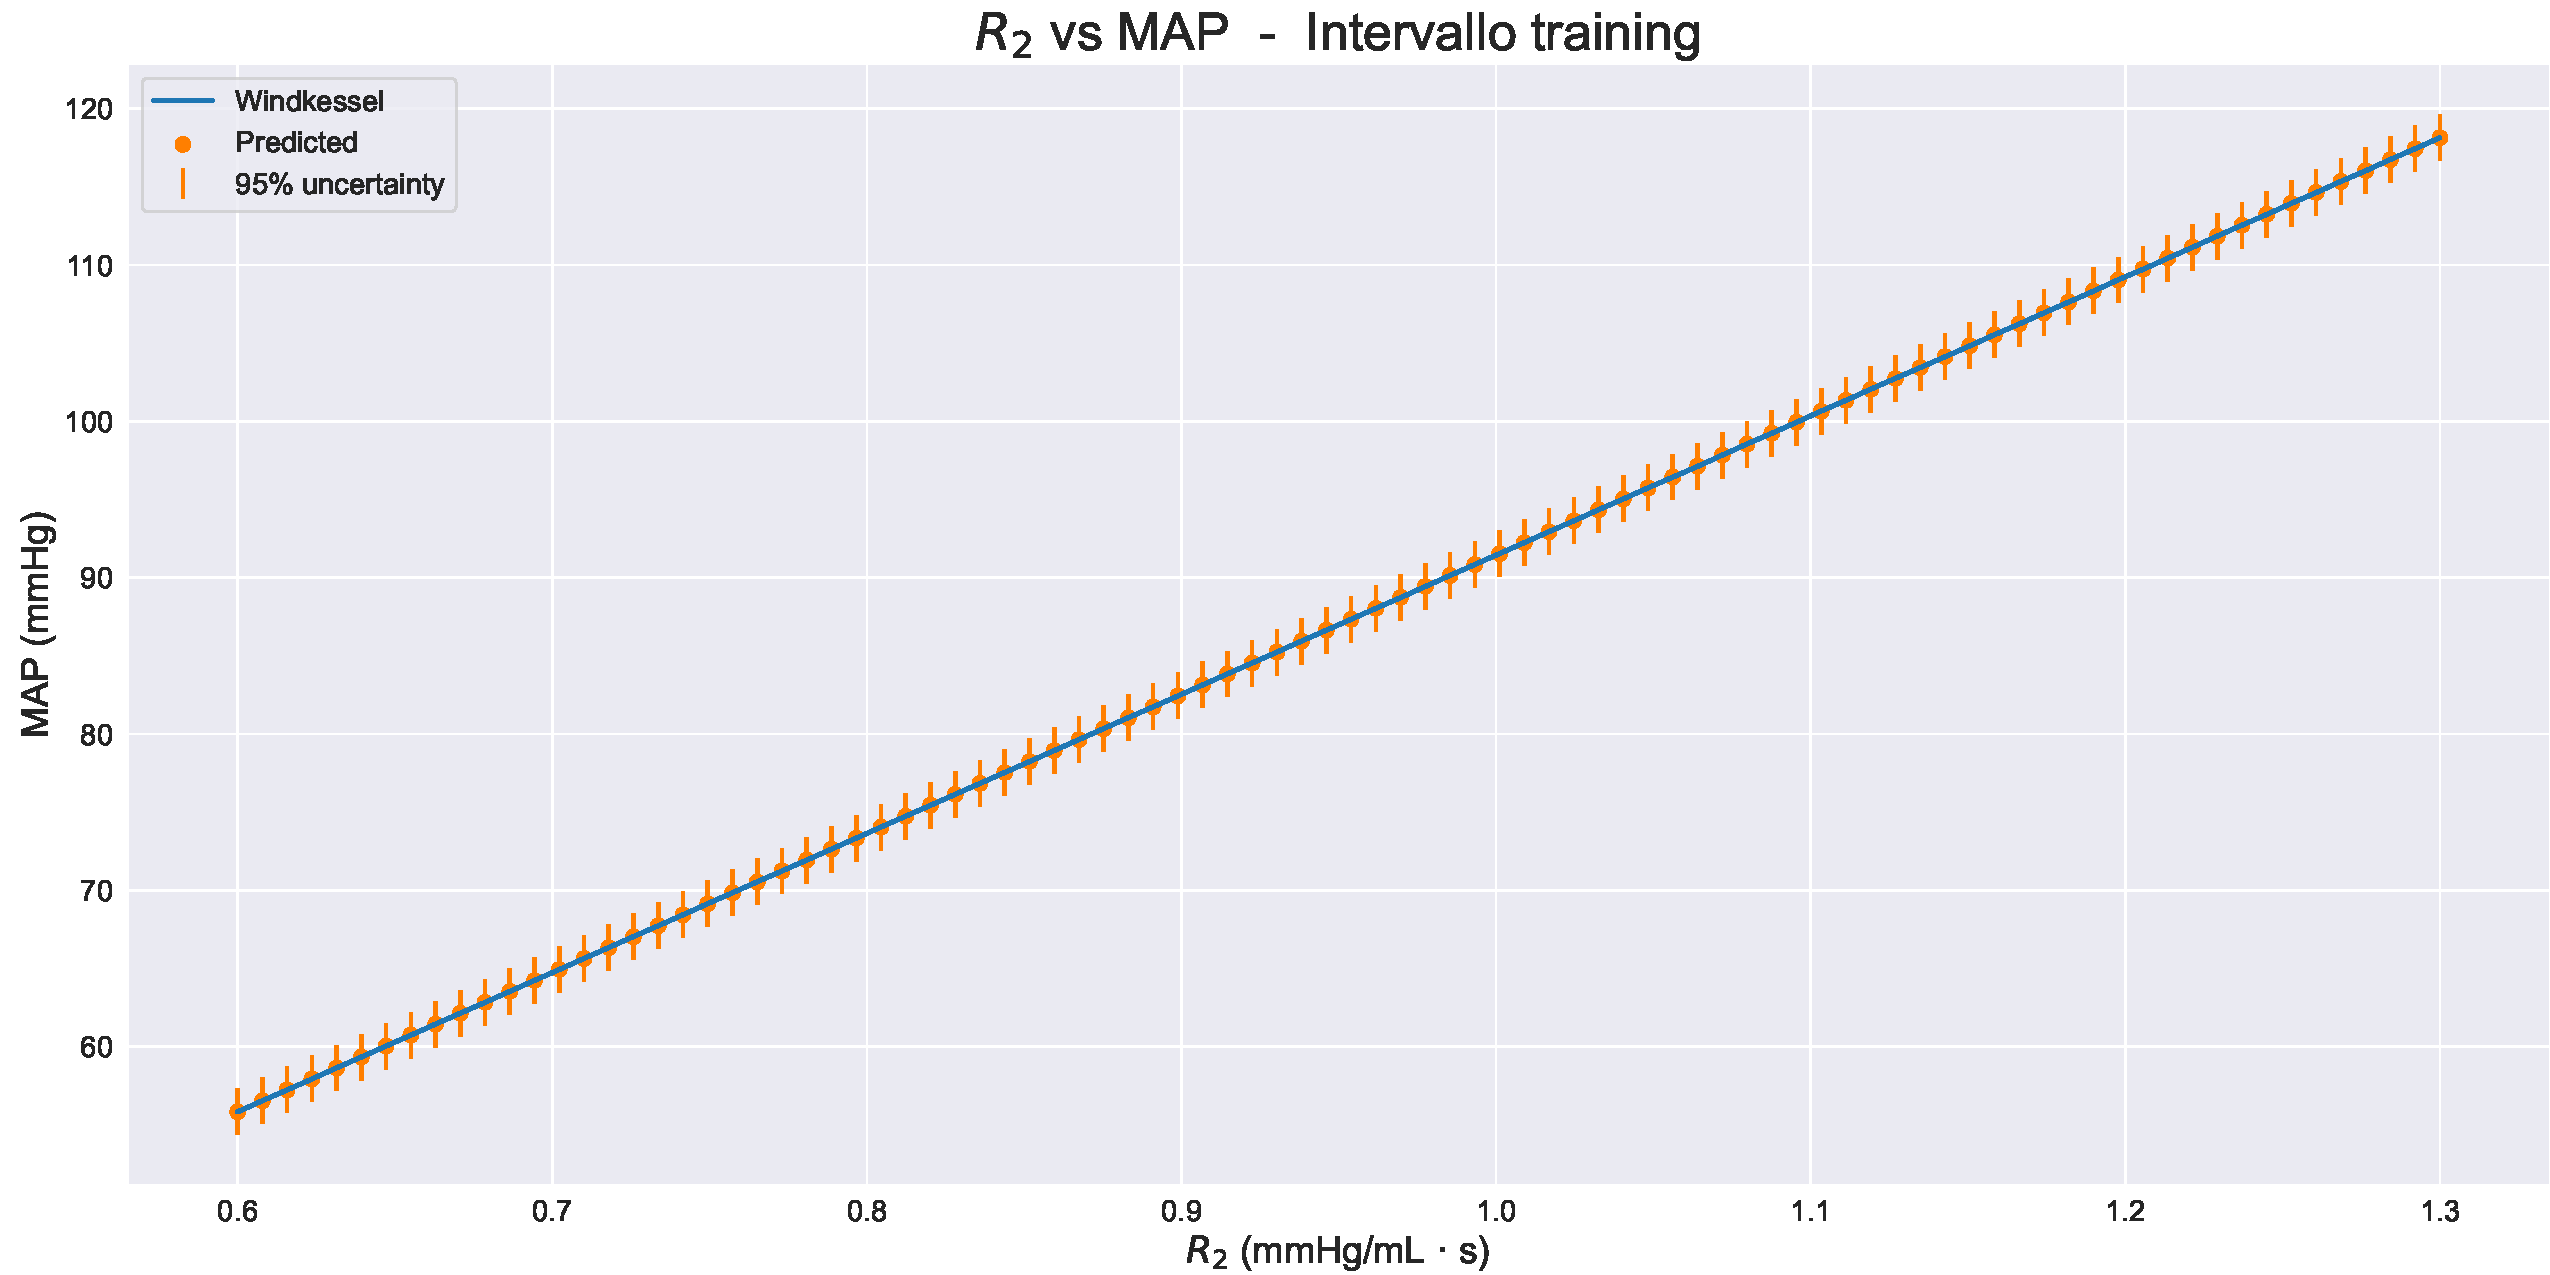
\includegraphics[width=1\textwidth]{images/Training (risultati)/MAP/MAP - R2 - training.pdf}
    \caption{Dependence of MAP on $R2$ over the training interval.}
    \label{MAP - R2 - training}
\end{figure}

\begin{figure}
    \centering
    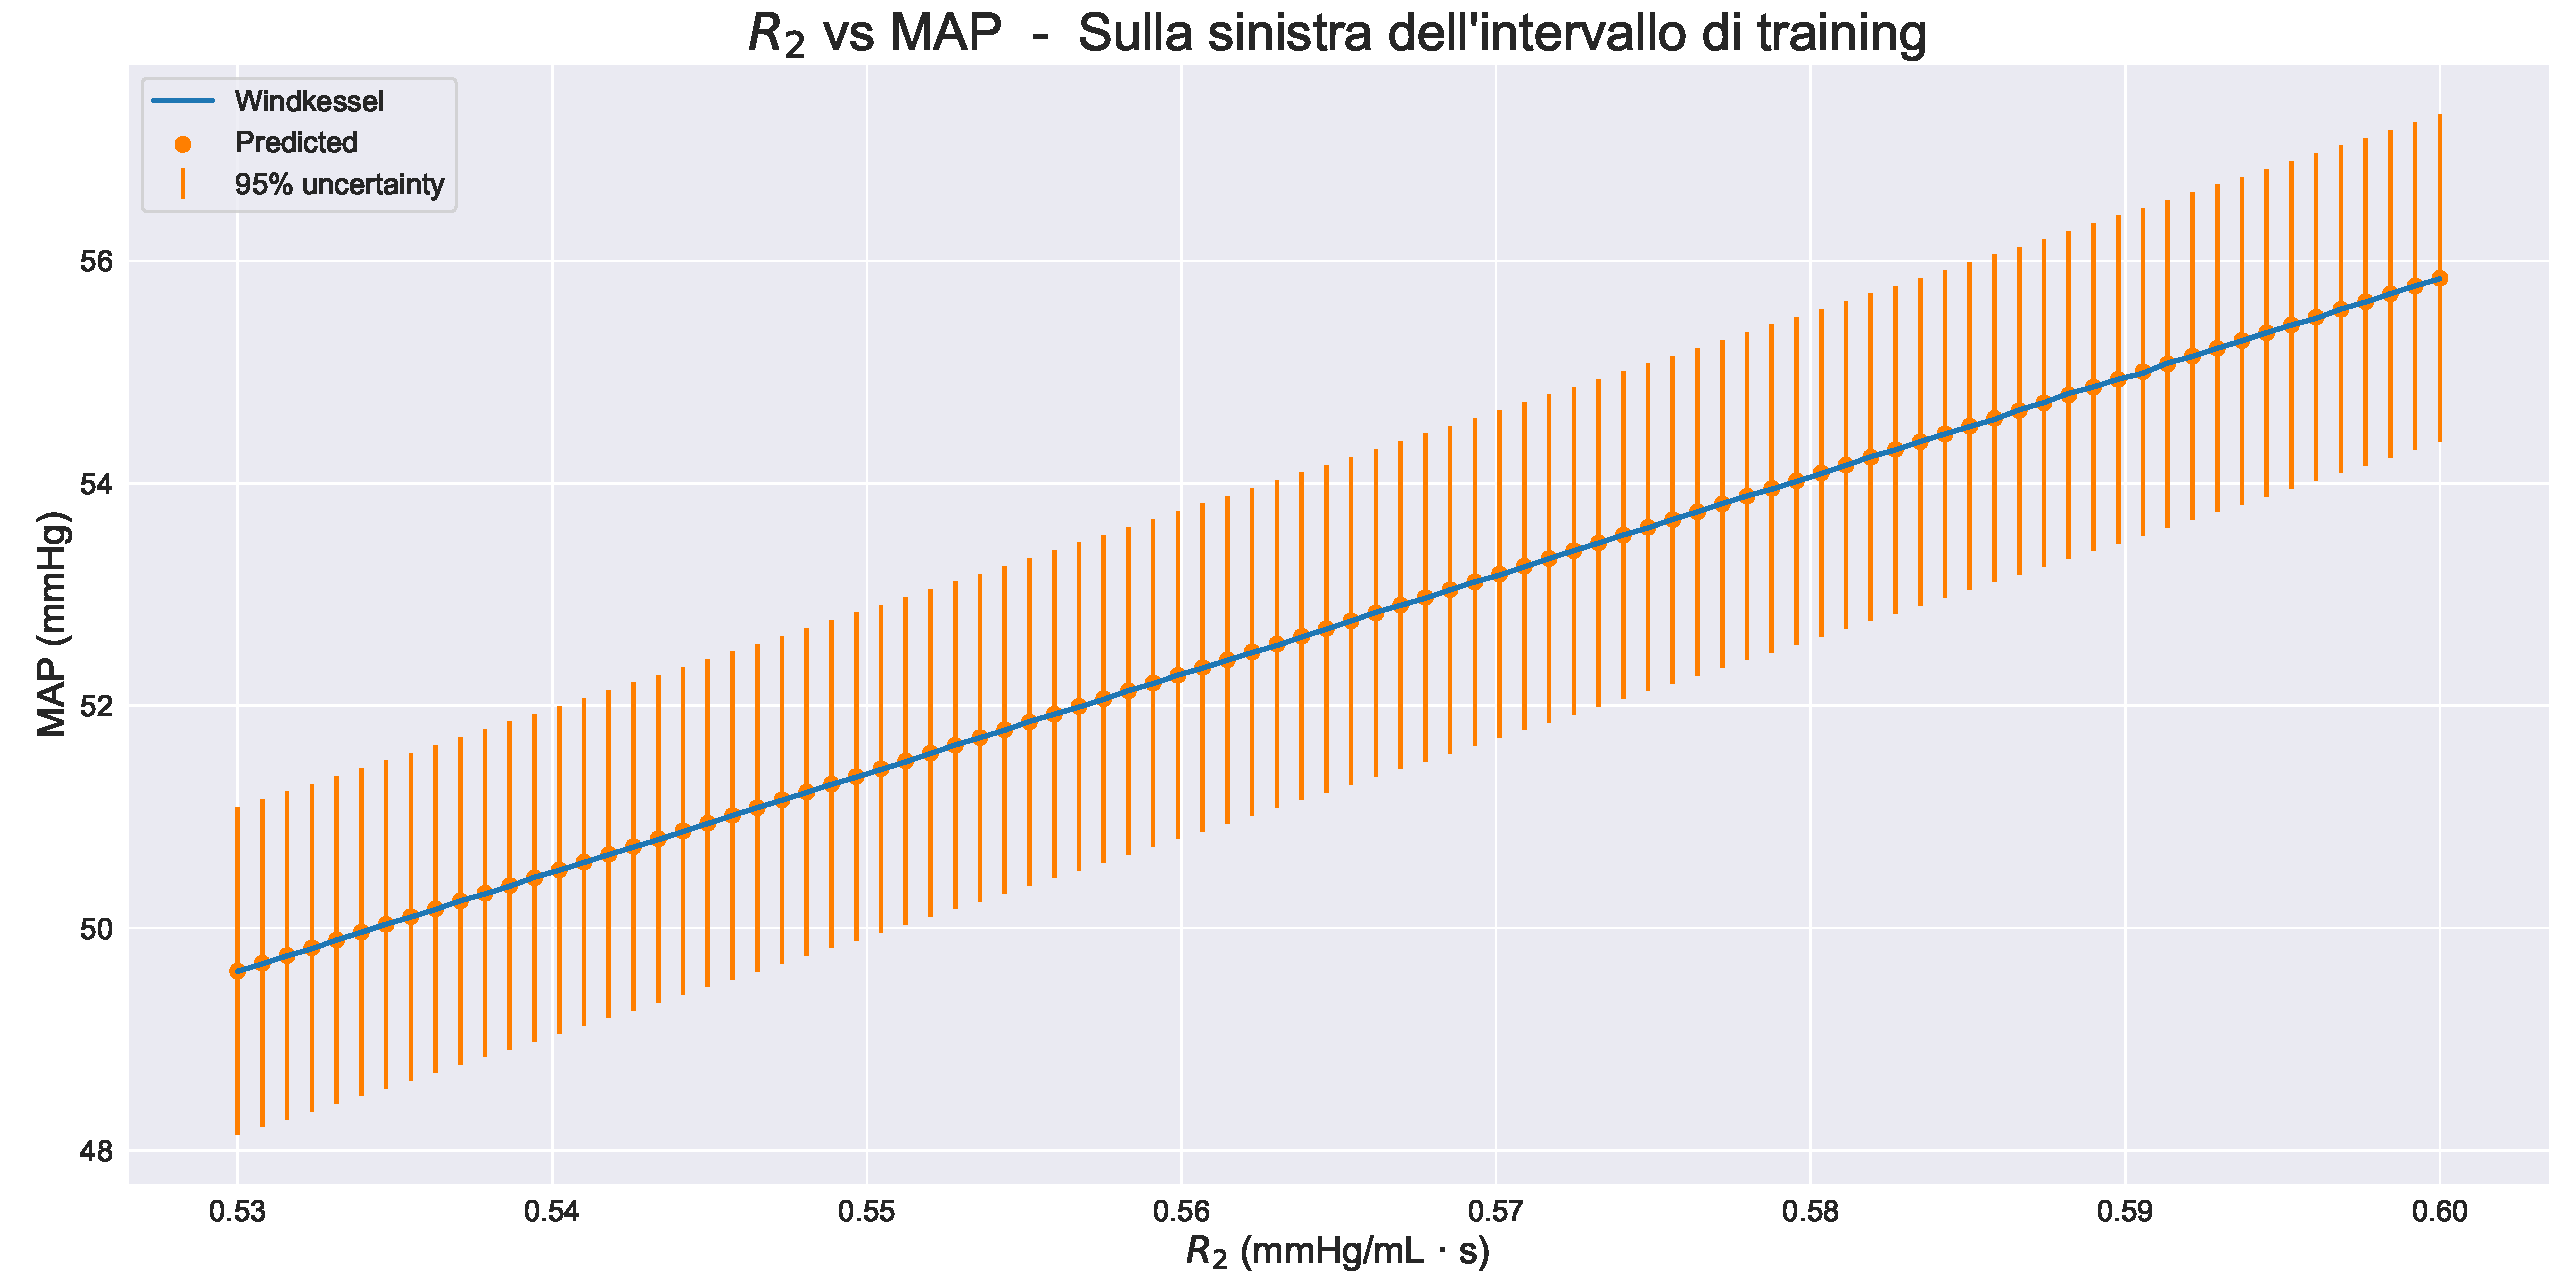
\includegraphics[width=1\textwidth]{images/Training (risultati)/MAP/MAP - R2 - sx.pdf}
    \caption{Dependence of MAP on $R2$ on the adjoint interval to the left of the training interval.}
    \label{MAP - R2 - sx}
\end{figure}


\begin{figure}
    \centering
    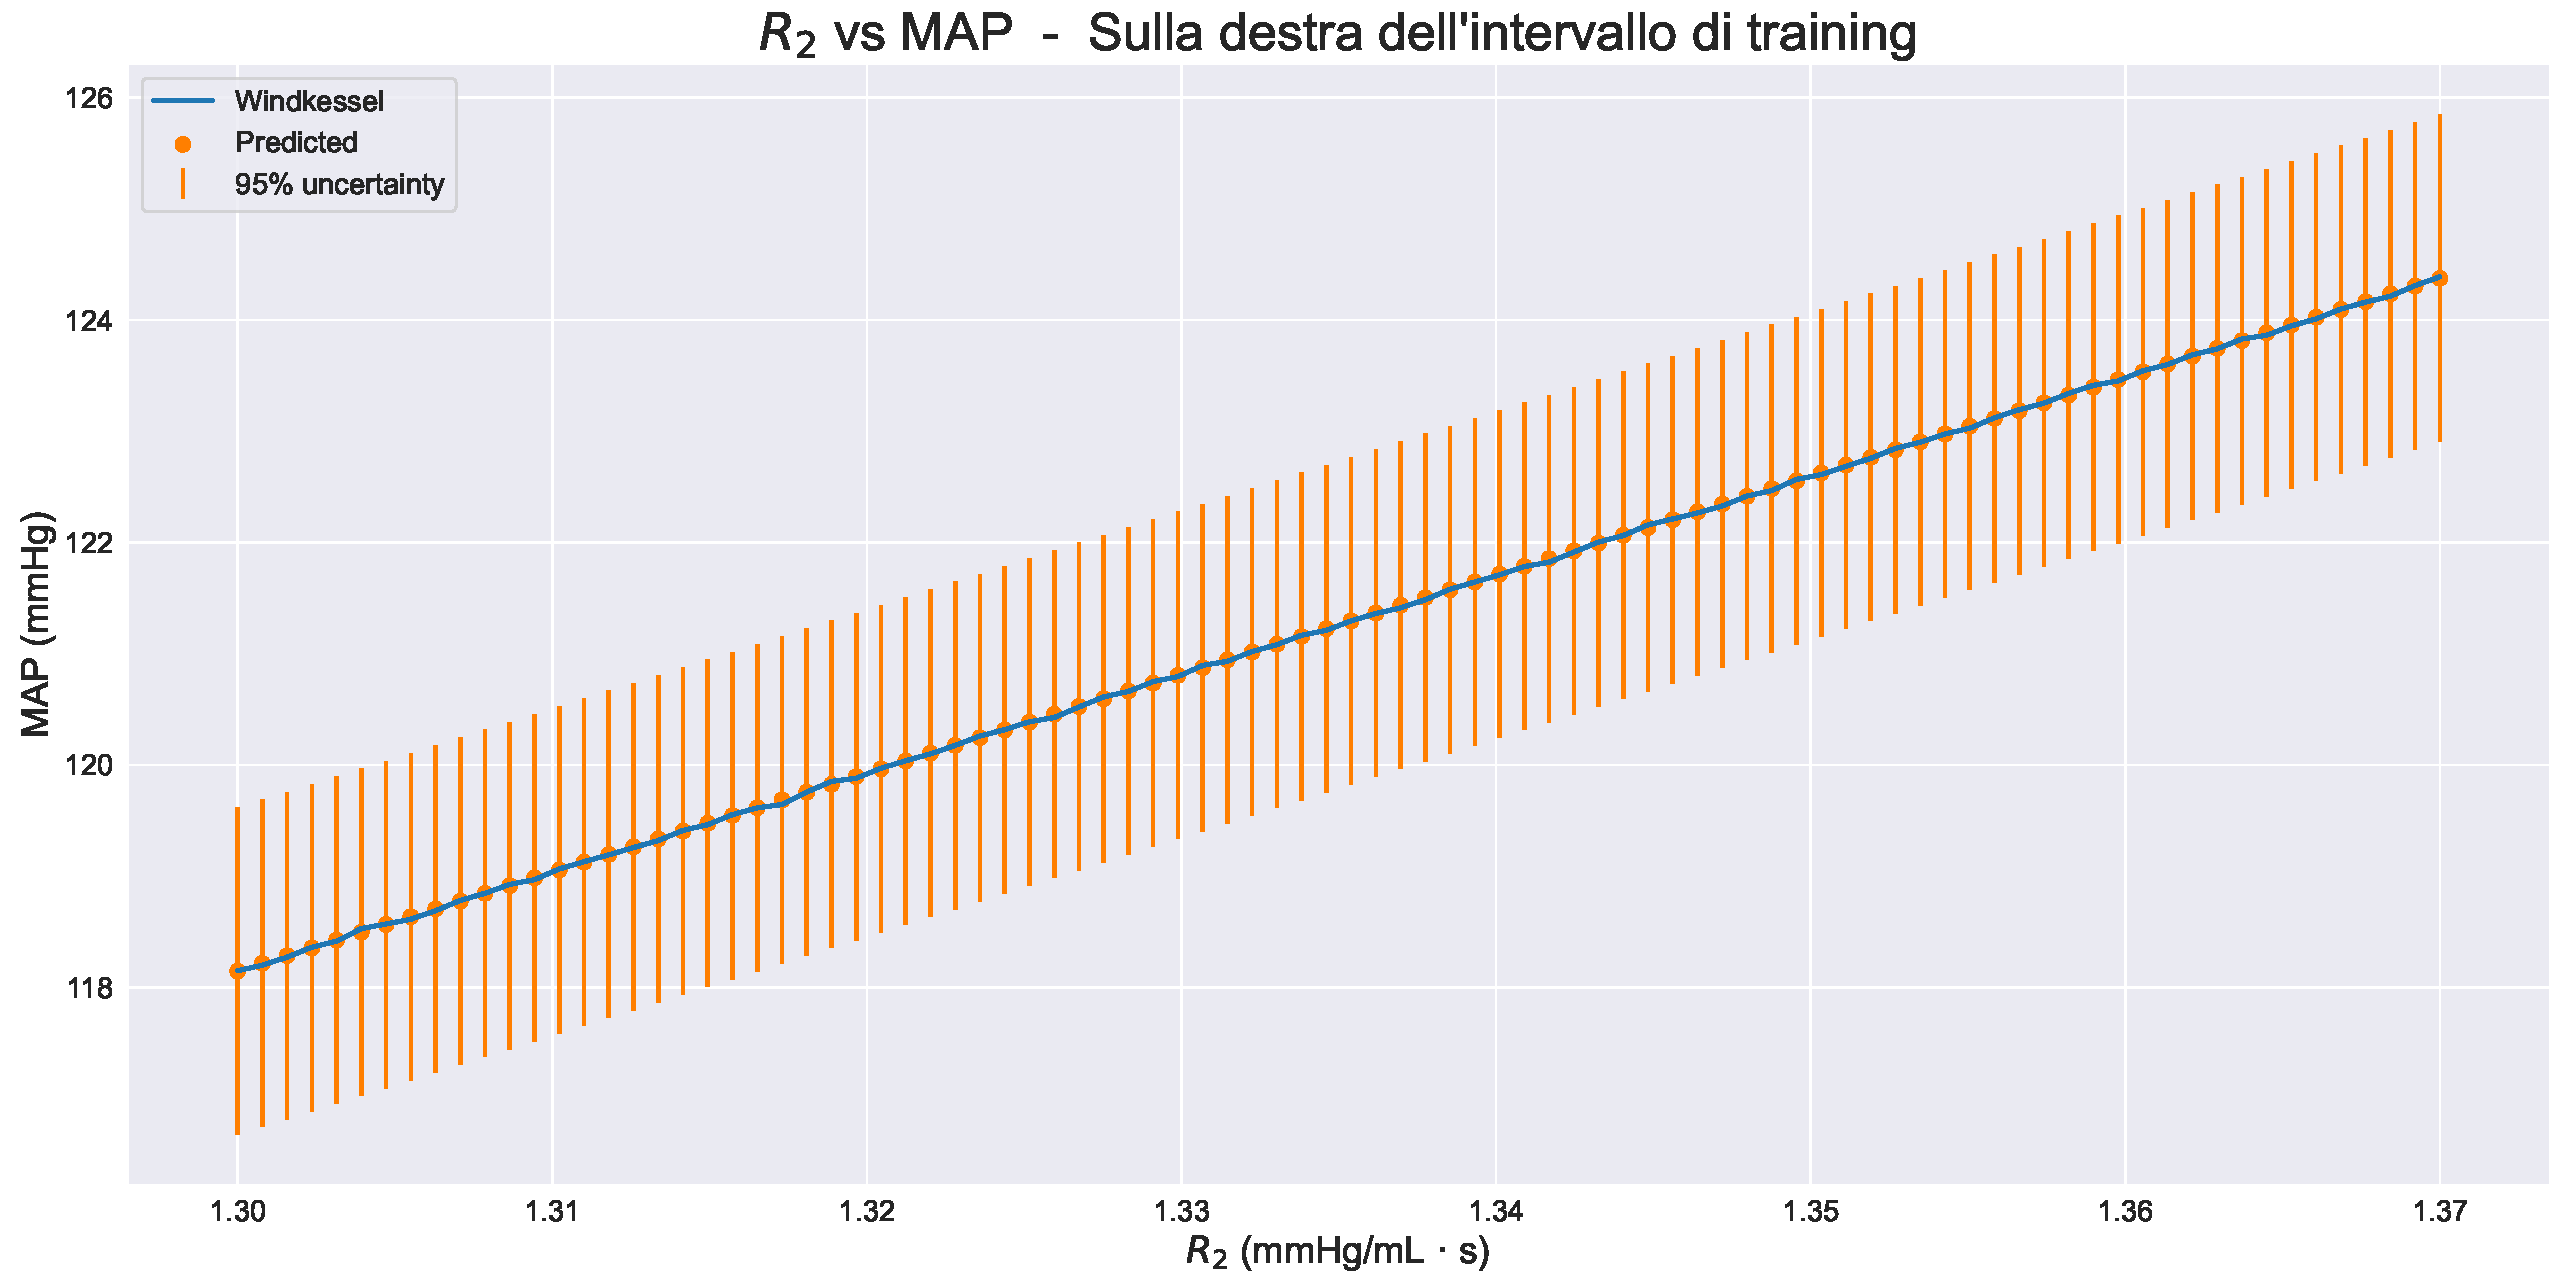
\includegraphics[width=1\textwidth]{images/Training (risultati)/MAP/MAP - R2 - dx.pdf}
    \caption{Dependence of MAP on $R2$ on the adjacent interval to the right of the training interval.}
    \label{MAP - R2 - dx}
\end{figure}







\newpage
%******************************
%*********** DBP **************
%******************************
\subsection{Diastolic blood pressure (DBP)}
$\text{lr}=0.07$ is imposed and the early stopper \textit{GLEarlyStoppingCriterion} is used with parameters: $\alpha = 2$, $\text{patience}=2$.



% **********
% DBP - loss
% **********
\subsubsection{Training and validation loss}
The training needed one hundred and thirty-one EPOCHS, concluded with $\text{R2Score}=0.9999$, $\text{MeanSquaredError}=0.0001$. Figure \ref{DBP - loss} shows the trend of training and validation loss with MSE and R2Score; in green is the trend of early stopper.
\begin{figure}[h]
    \centering
    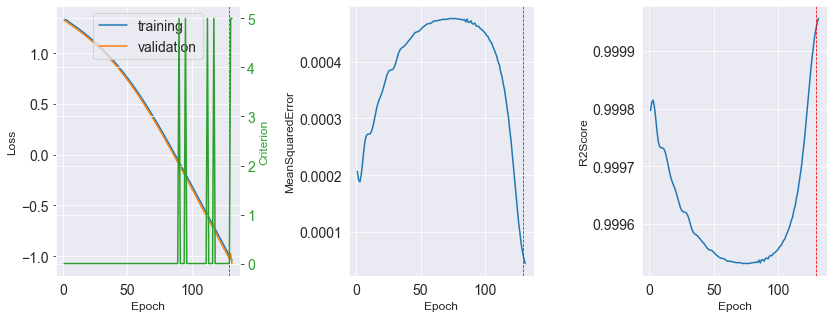
\includegraphics[width=1\textwidth]{images/Training (risultati)/DBP/DBP - loss.png}
    \caption{DBP: progress of training and validation loss, early stopper, R2Score e MSE.}
    \label{DBP - loss}
\end{figure}

\vspace{-0.5cm}

% **********
% DBP - inference
% **********
\subsubsection{Approximation of input data}
Figure \ref{DBP - inference} shows how the predictions approximate the input data. The length of the error bars is $0.0028$.

\begin{figure}[h]
    \centering
    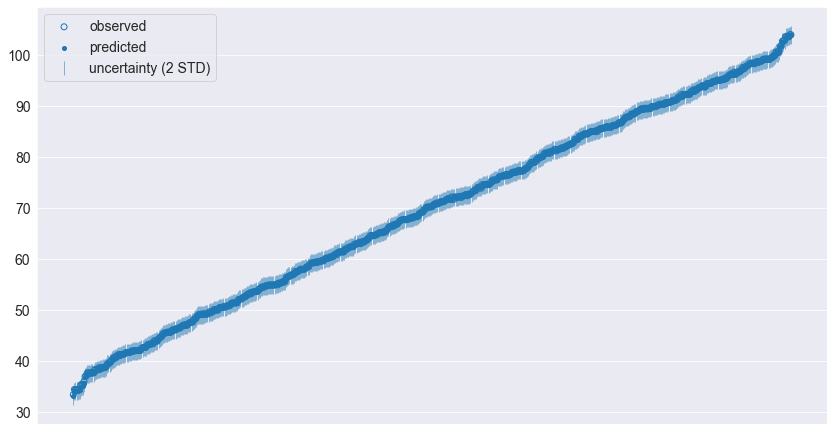
\includegraphics[width=1\textwidth]{images/Training (risultati)/DBP/DBP - inference.png}
    \caption{DBP: input data predictions.}
    \label{DBP - inference}
\end{figure}



% **********
% DBP - C
% **********
\subsubsection{Dependence on $C$}
The overall result is shown in figure \ref{DBP - C - full}, the result in the training interval alone in \ref{DBP - C - training}, the result in the individual adjacent intervals in \ref{DBP - C - sx} and \ref{DBP - C - dx}. In all intervals the model succeeds in generating excellent predictions with low uncertainty (represented by the error bars).

\vspace{1cm}

\begin{figure}[!htb]
    \centering
    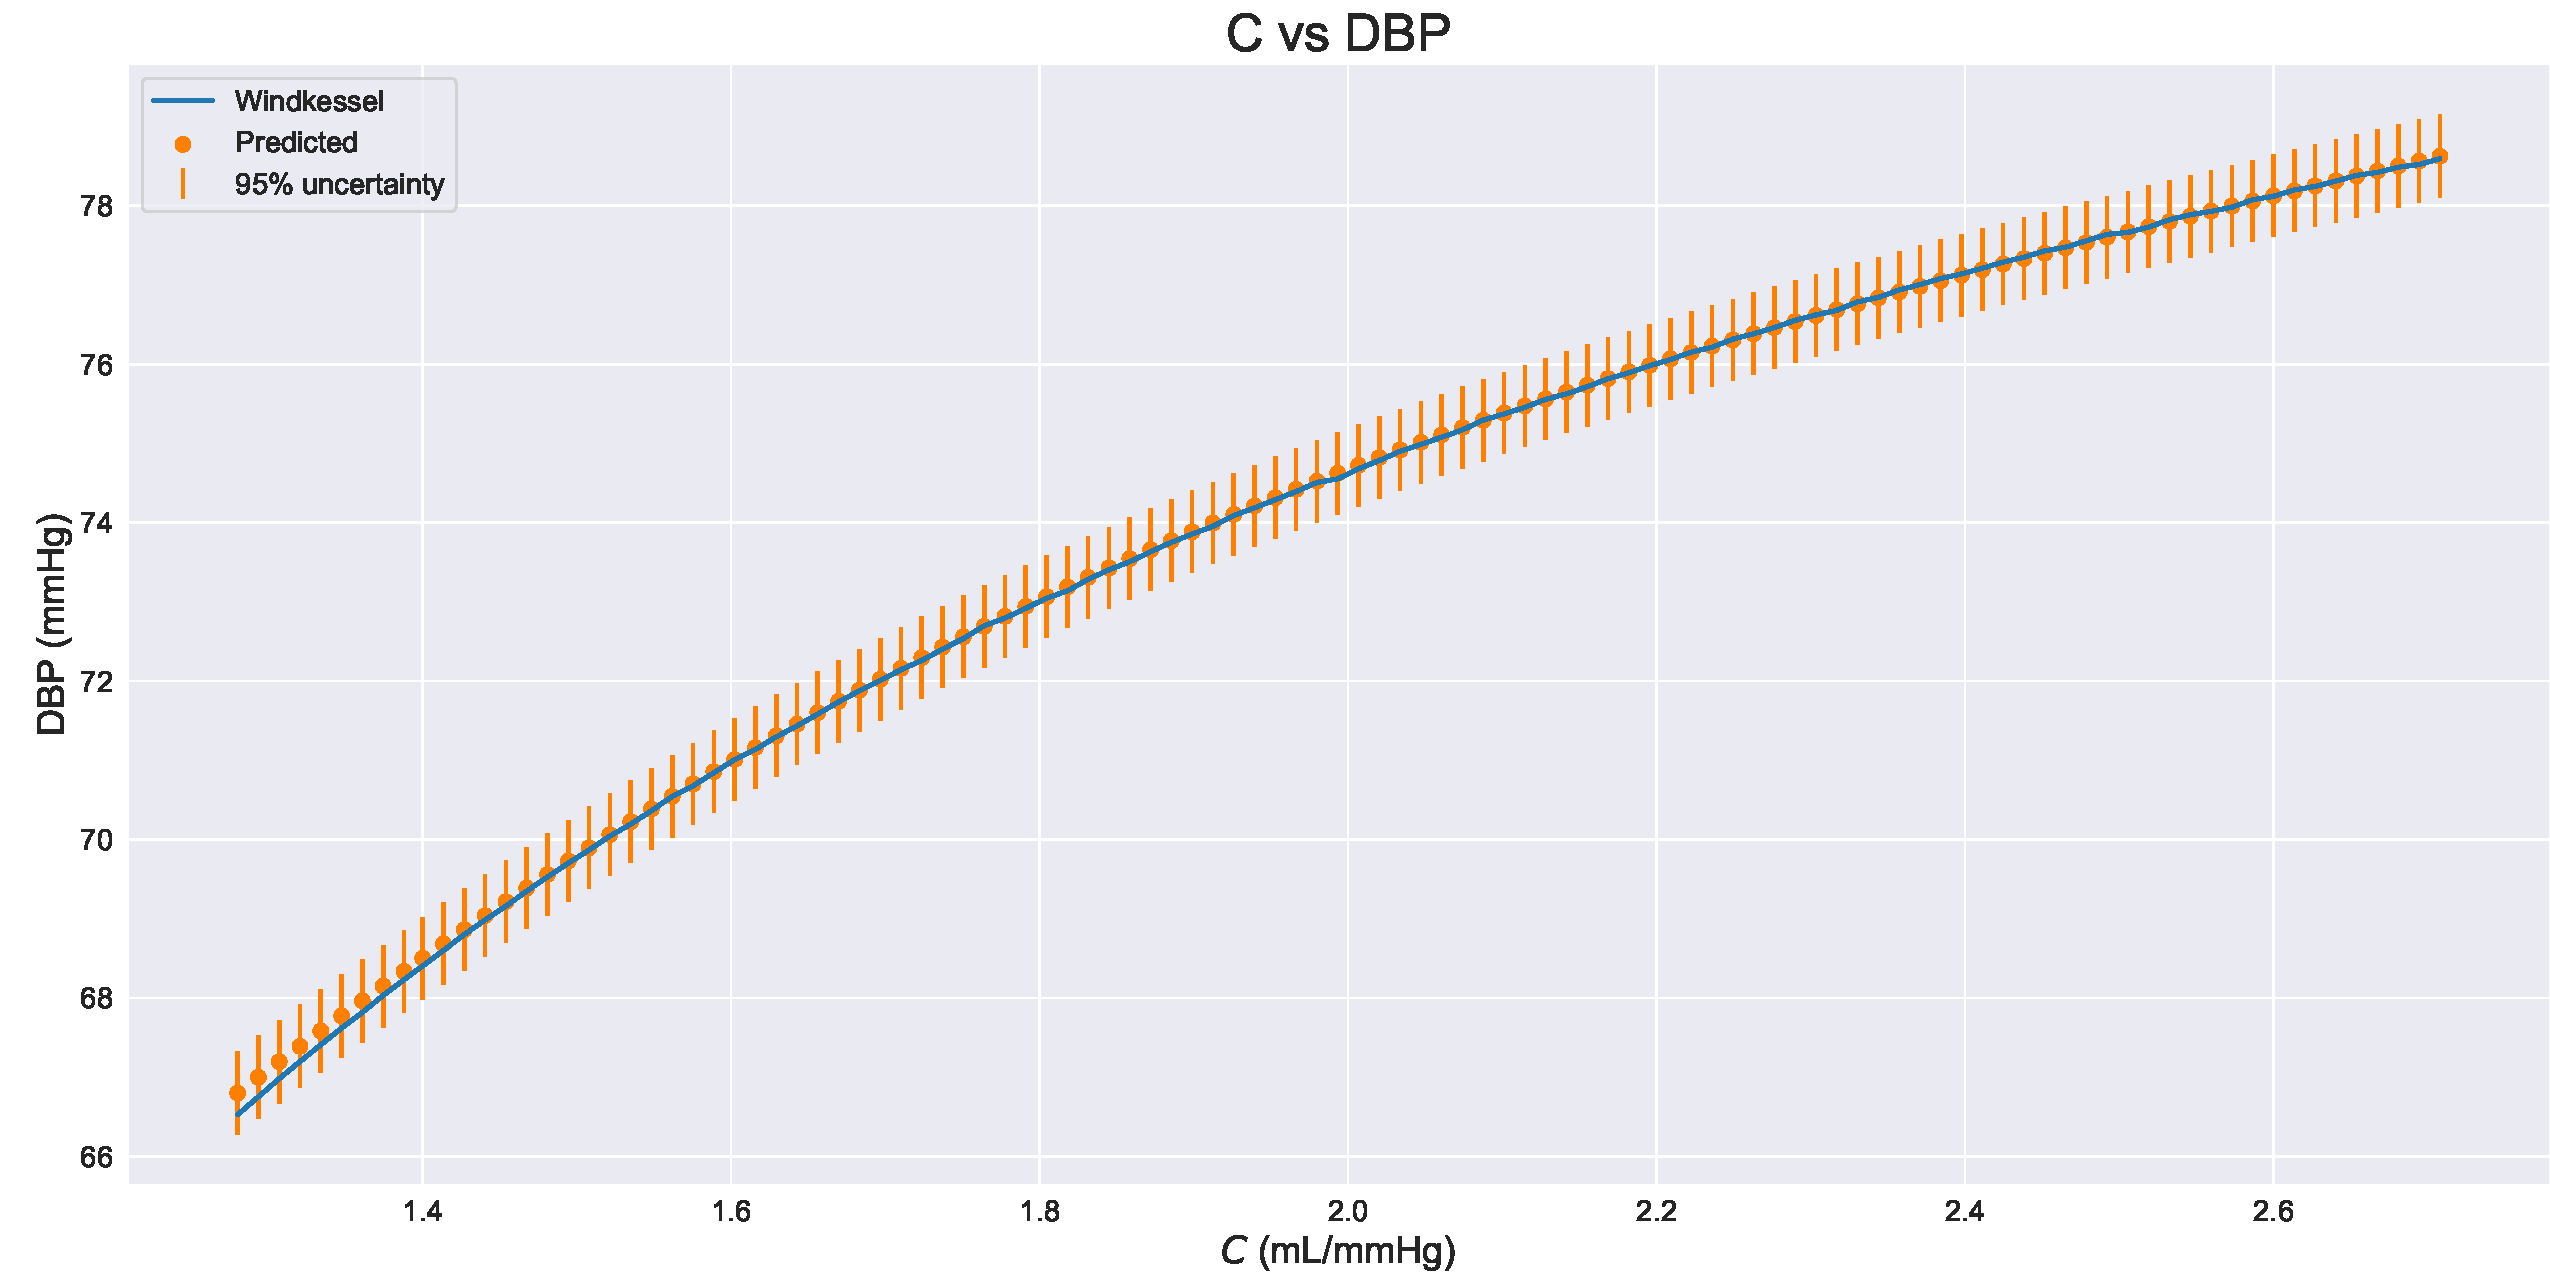
\includegraphics[width=1\textwidth]{images/Training (risultati)/DBP/DBP - C - full.pdf}
    \caption{Dependence of DBP on $C$ on the training interval and two adjacent intervals.}
    \label{DBP - C - full}
\end{figure}

\vspace{0.32cm}

\begin{figure}[!htb]
    \centering
    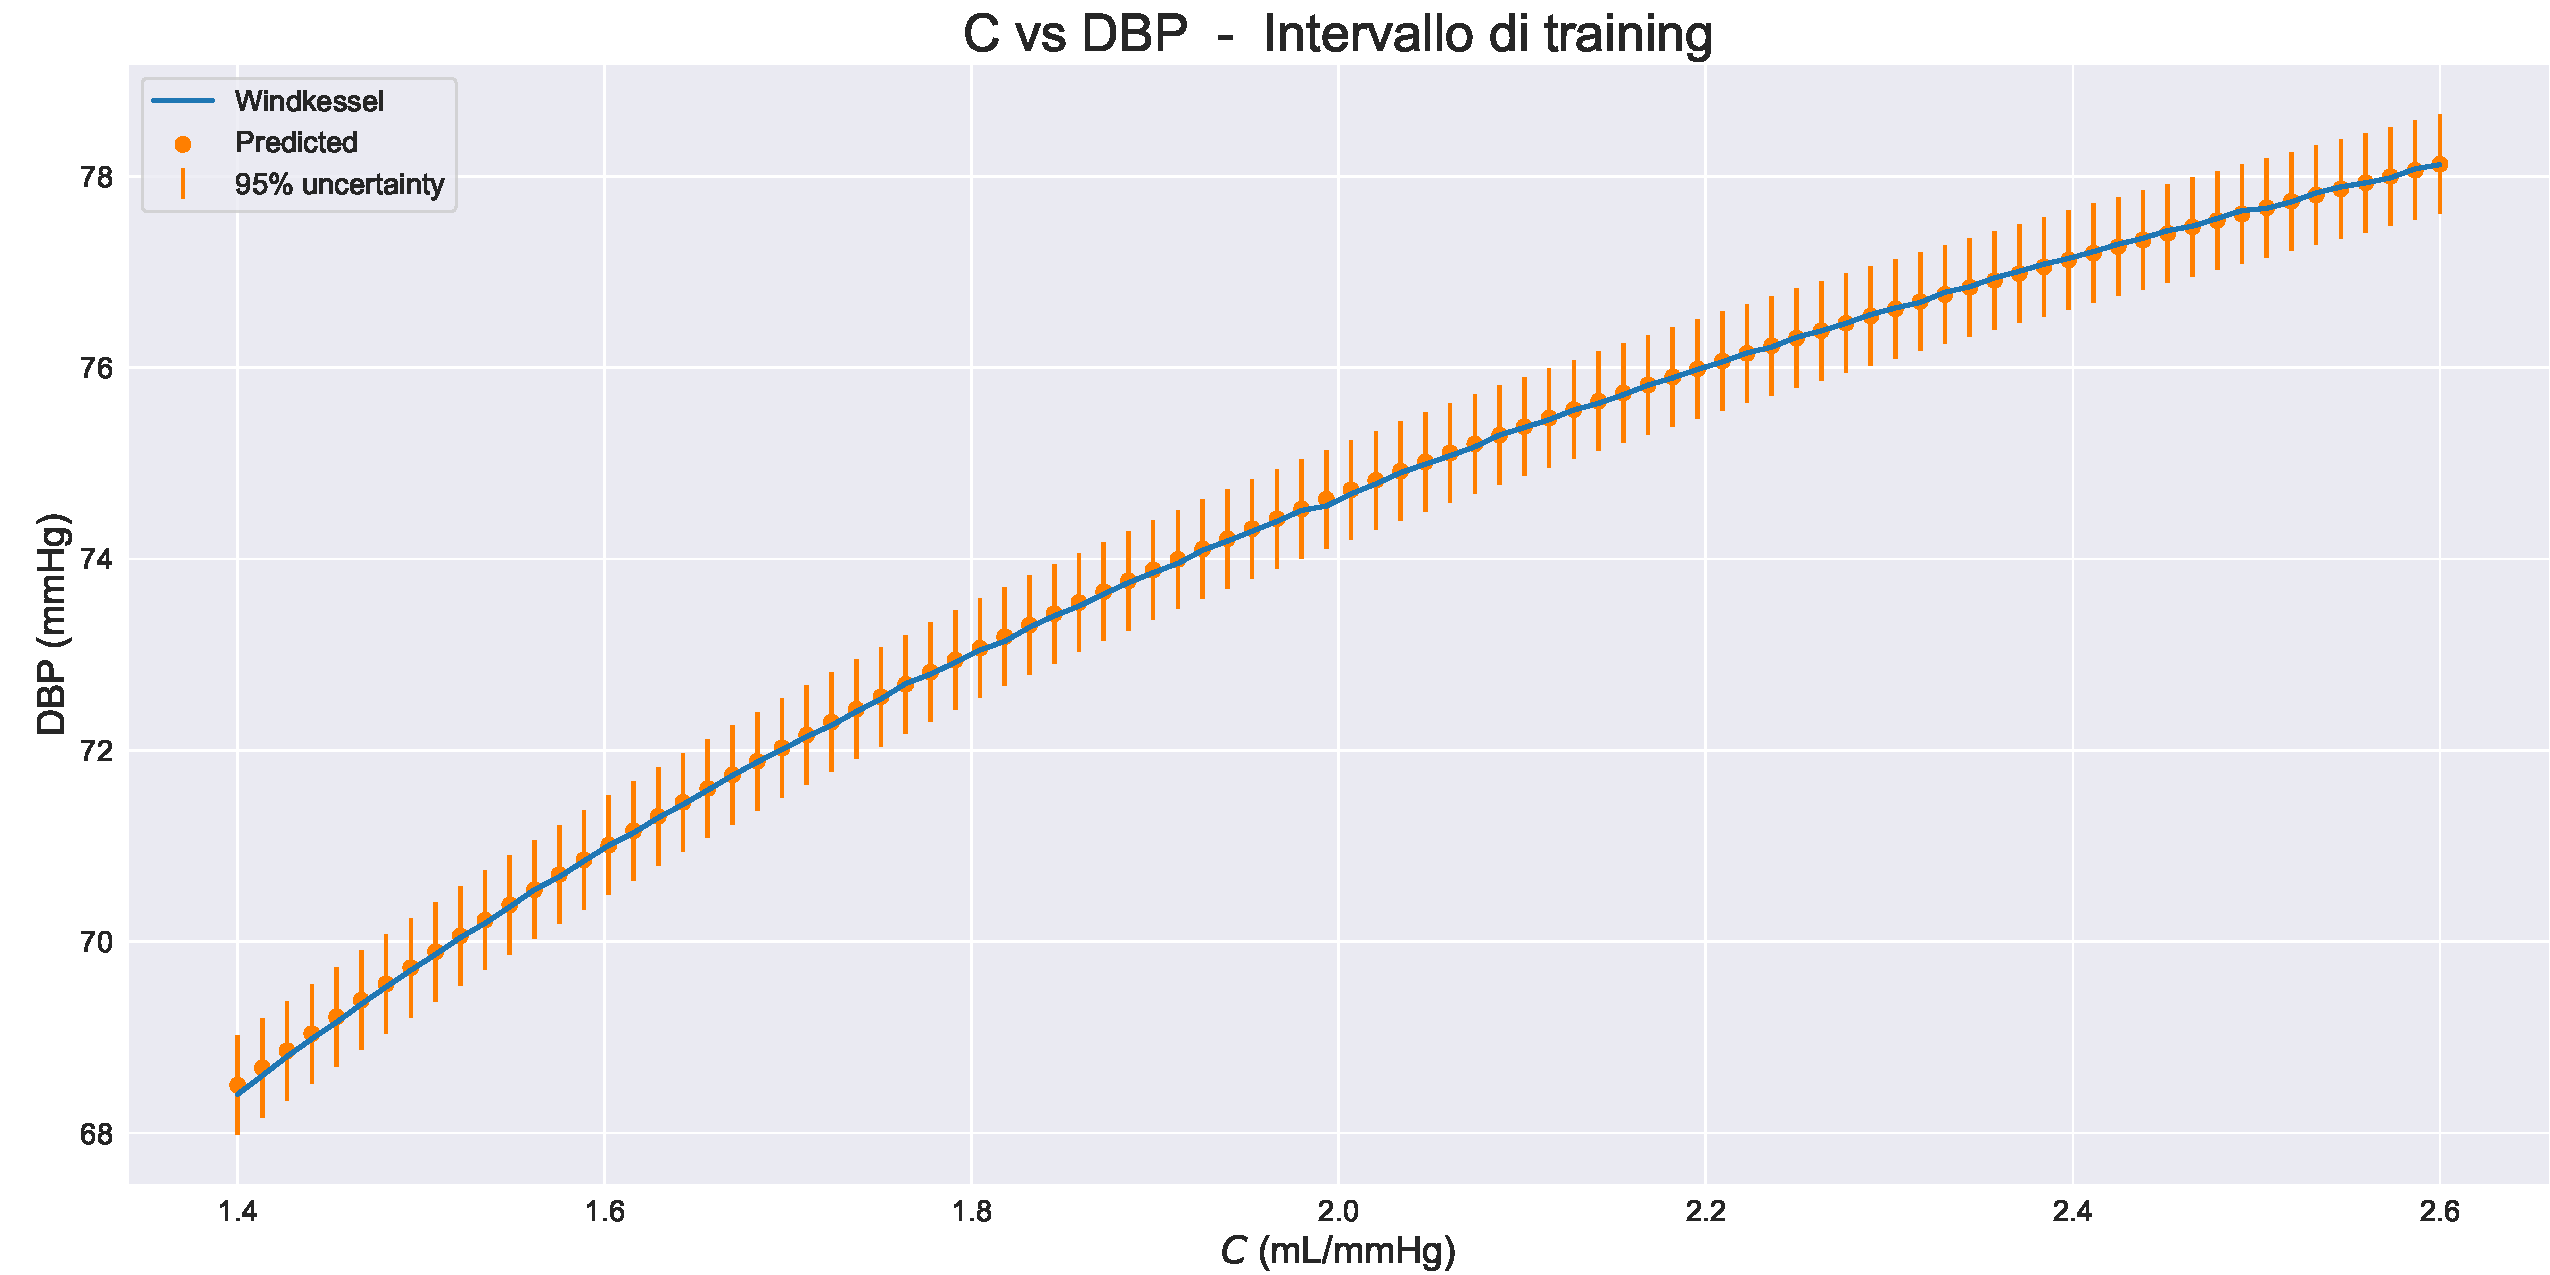
\includegraphics[width=1\textwidth]{images/Training (risultati)/DBP/DBP - C - training.pdf}
    \caption{Dependence of DBP on $C$ over the training interval.}
    \label{DBP - C - training}
\end{figure}



\begin{figure}
    \centering
    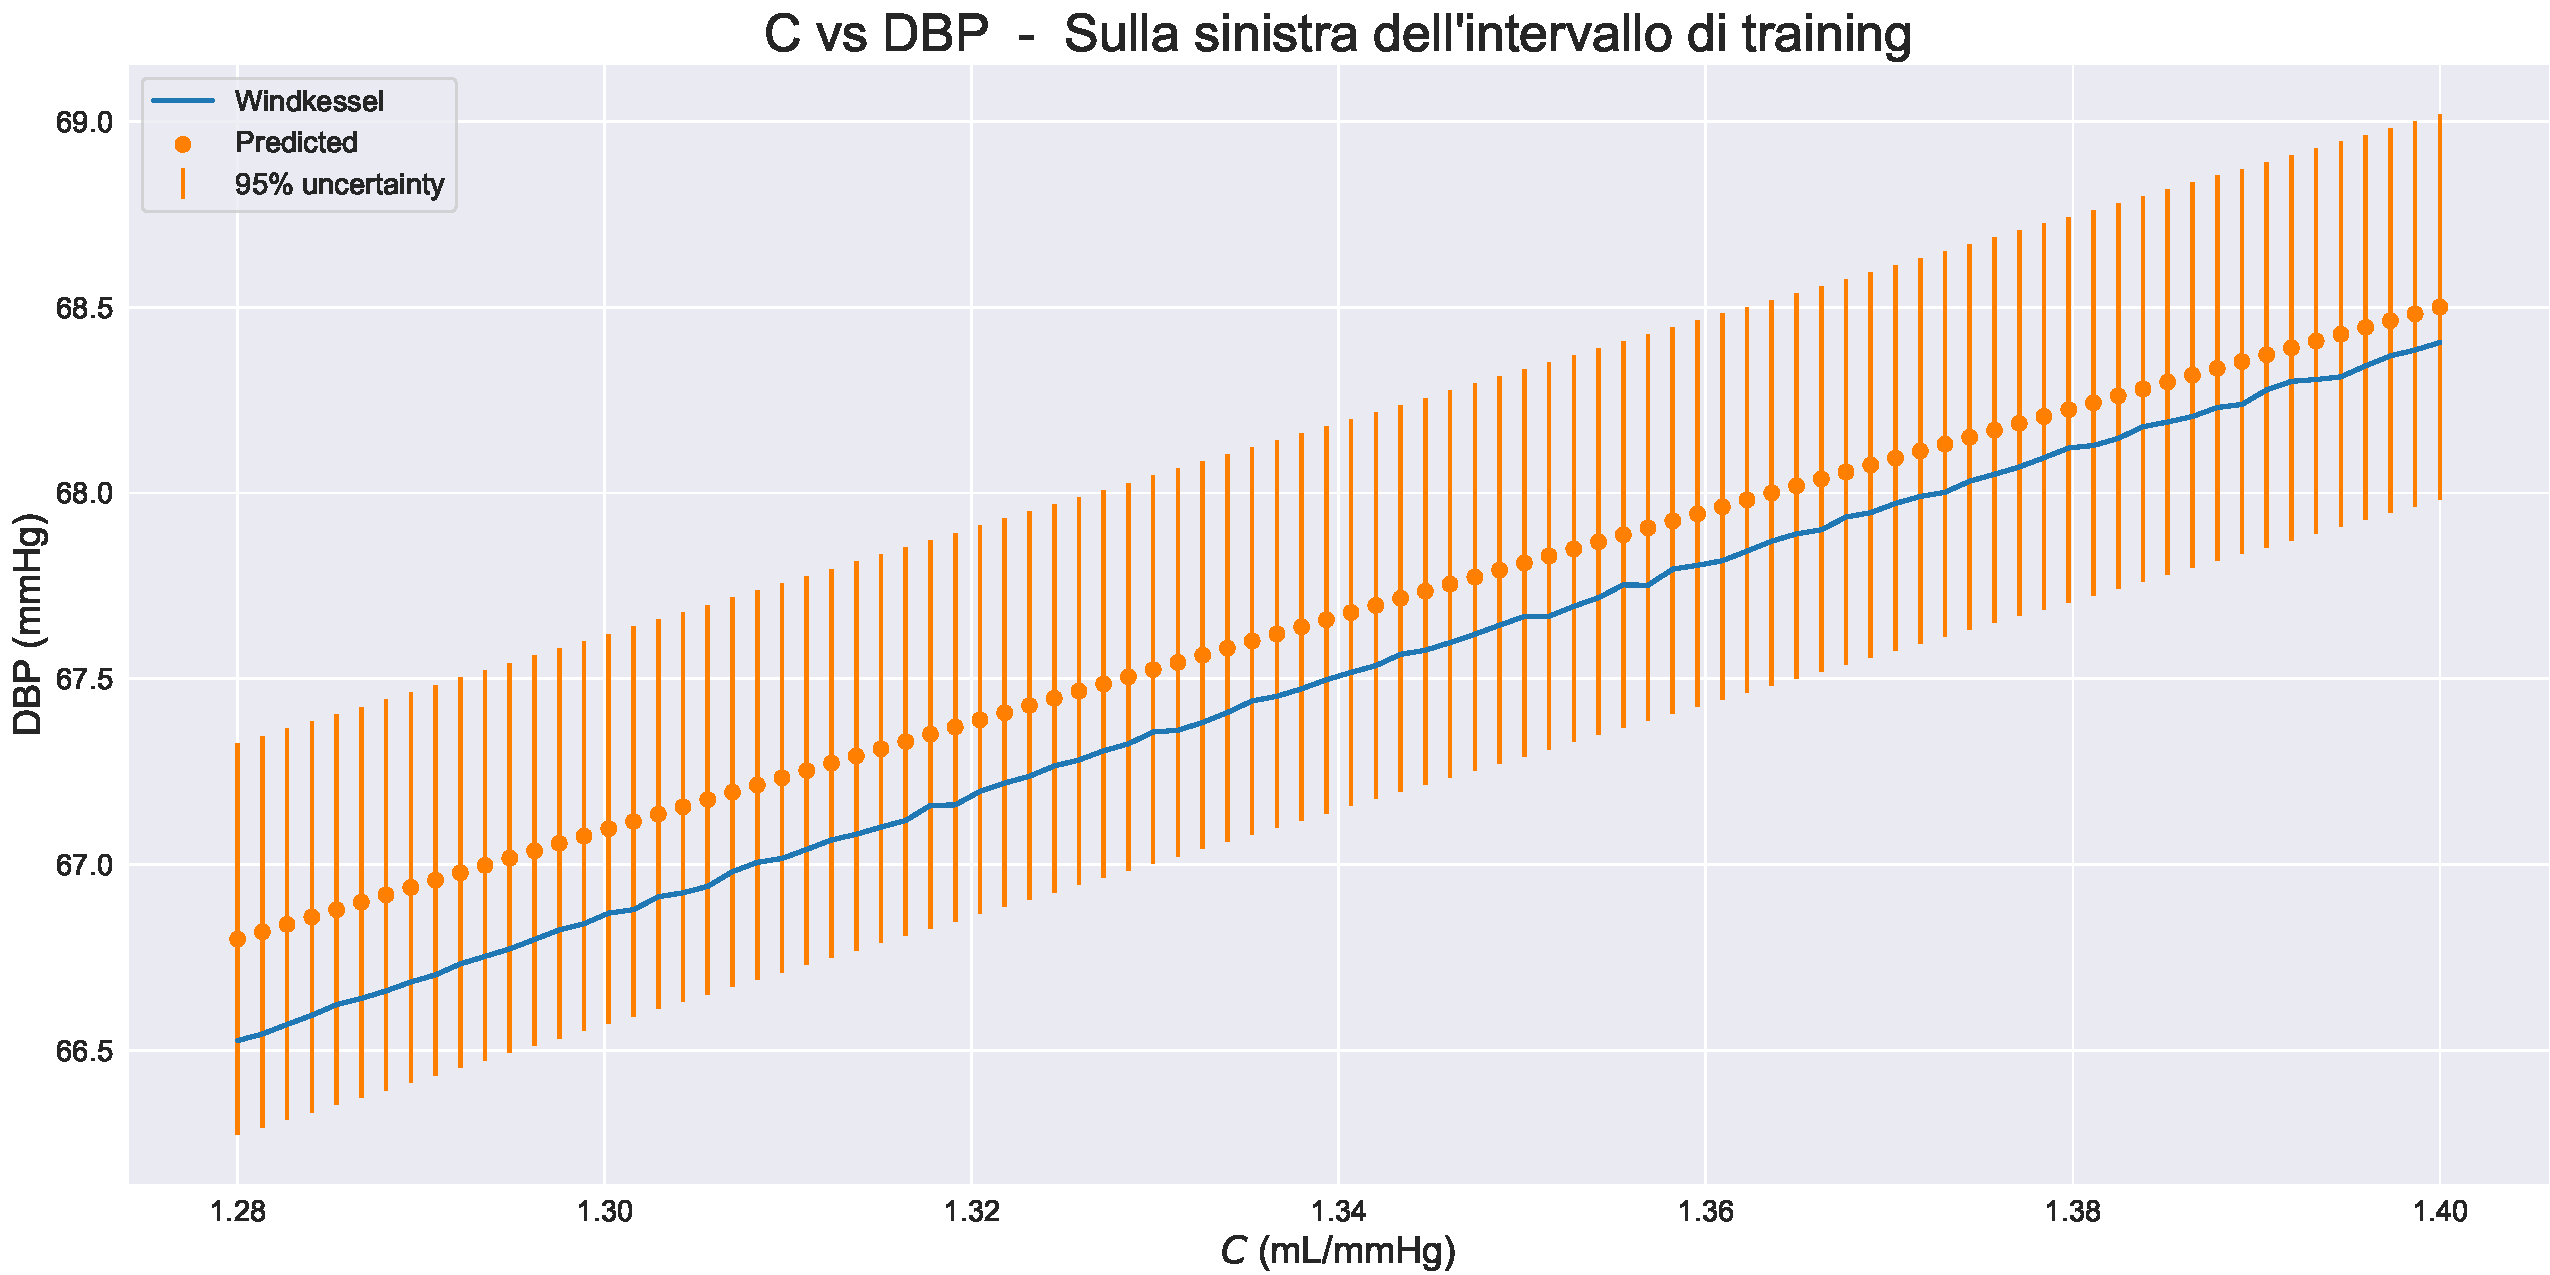
\includegraphics[width=1\textwidth]{images/Training (risultati)/DBP/DBP - C - sx.pdf}
    \caption{Dependence of DBP on $C$ on the adjacent interval to the left of the training interval.}
    \label{DBP - C - sx}
\end{figure}


\begin{figure}
    \centering
    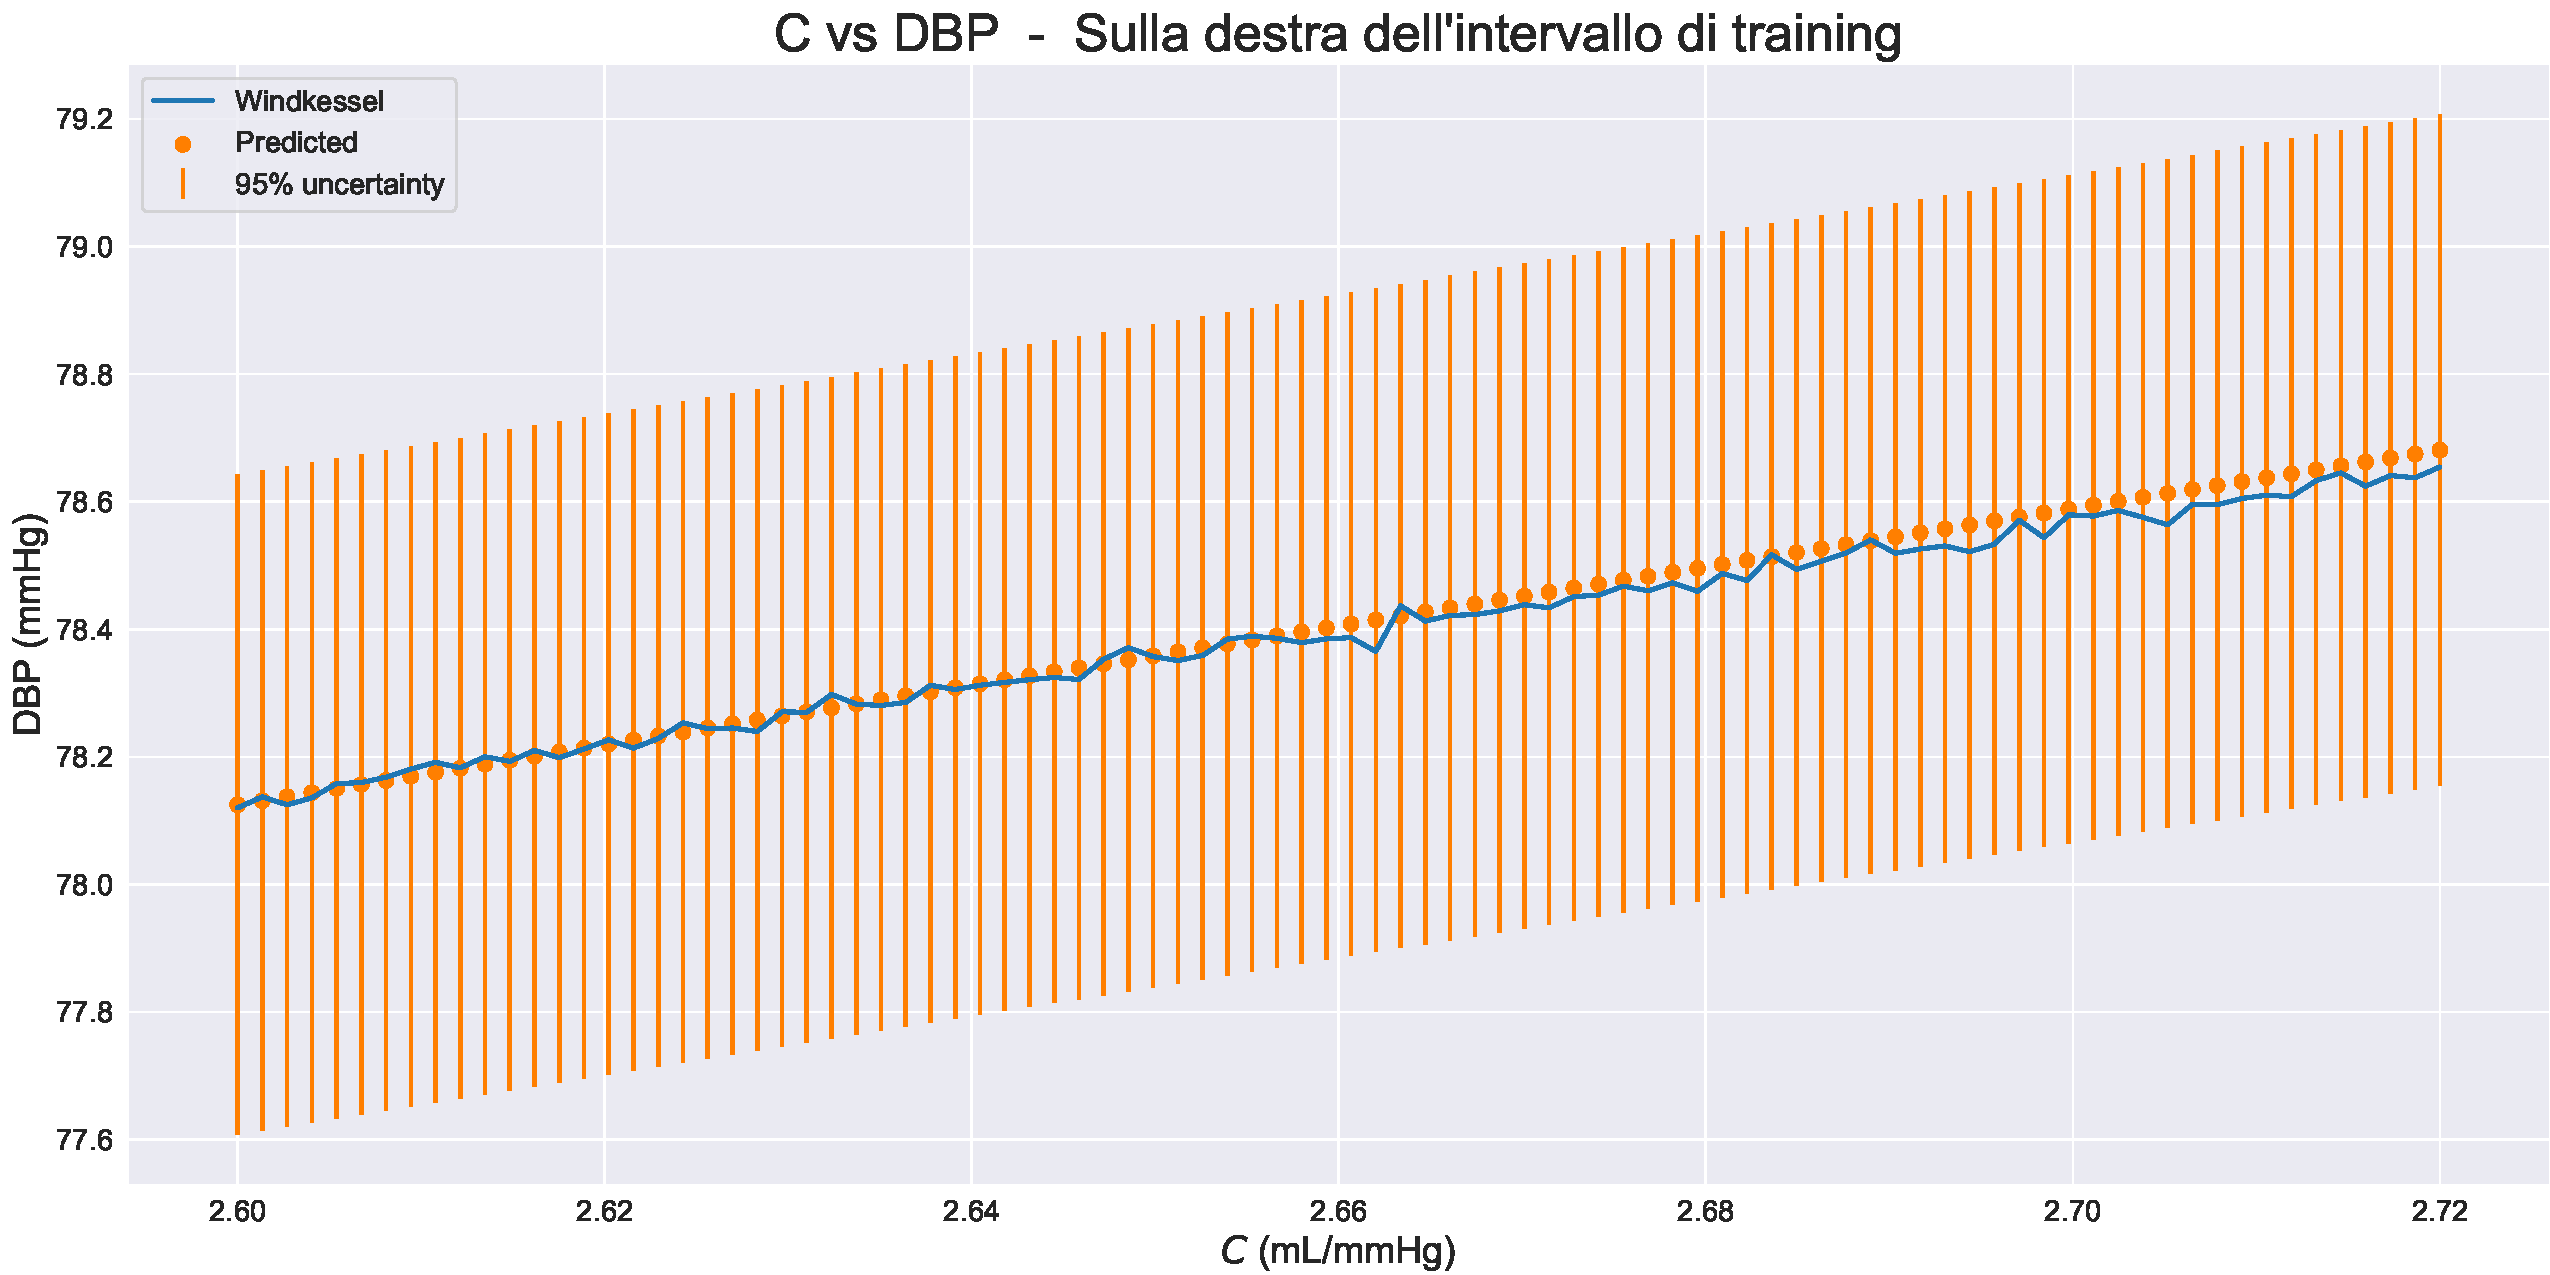
\includegraphics[width=1\textwidth]{images/Training (risultati)/DBP/DBP - C - dx.pdf}
    \caption{Dependence of DBP on $C$ on the adjacent interval to the right of the training interval.}
    \label{DBP - C - dx}
\end{figure}


\newpage

% **********
% DBP - R1
% **********
\subsubsection{Dependence on $R_1$}
The overall result is shown in figure \ref{DBP - R1 - full}, the result in the training interval alone in \ref{DBP - R1 - training}, the result in the individual adjacent intervals in \ref{DBP - R1 - sx} and \ref{DBP - R1 - dx}. Again, the model is able to make very accurate predictions.

\vspace{1cm}

\begin{figure}[!htb]
    \centering
    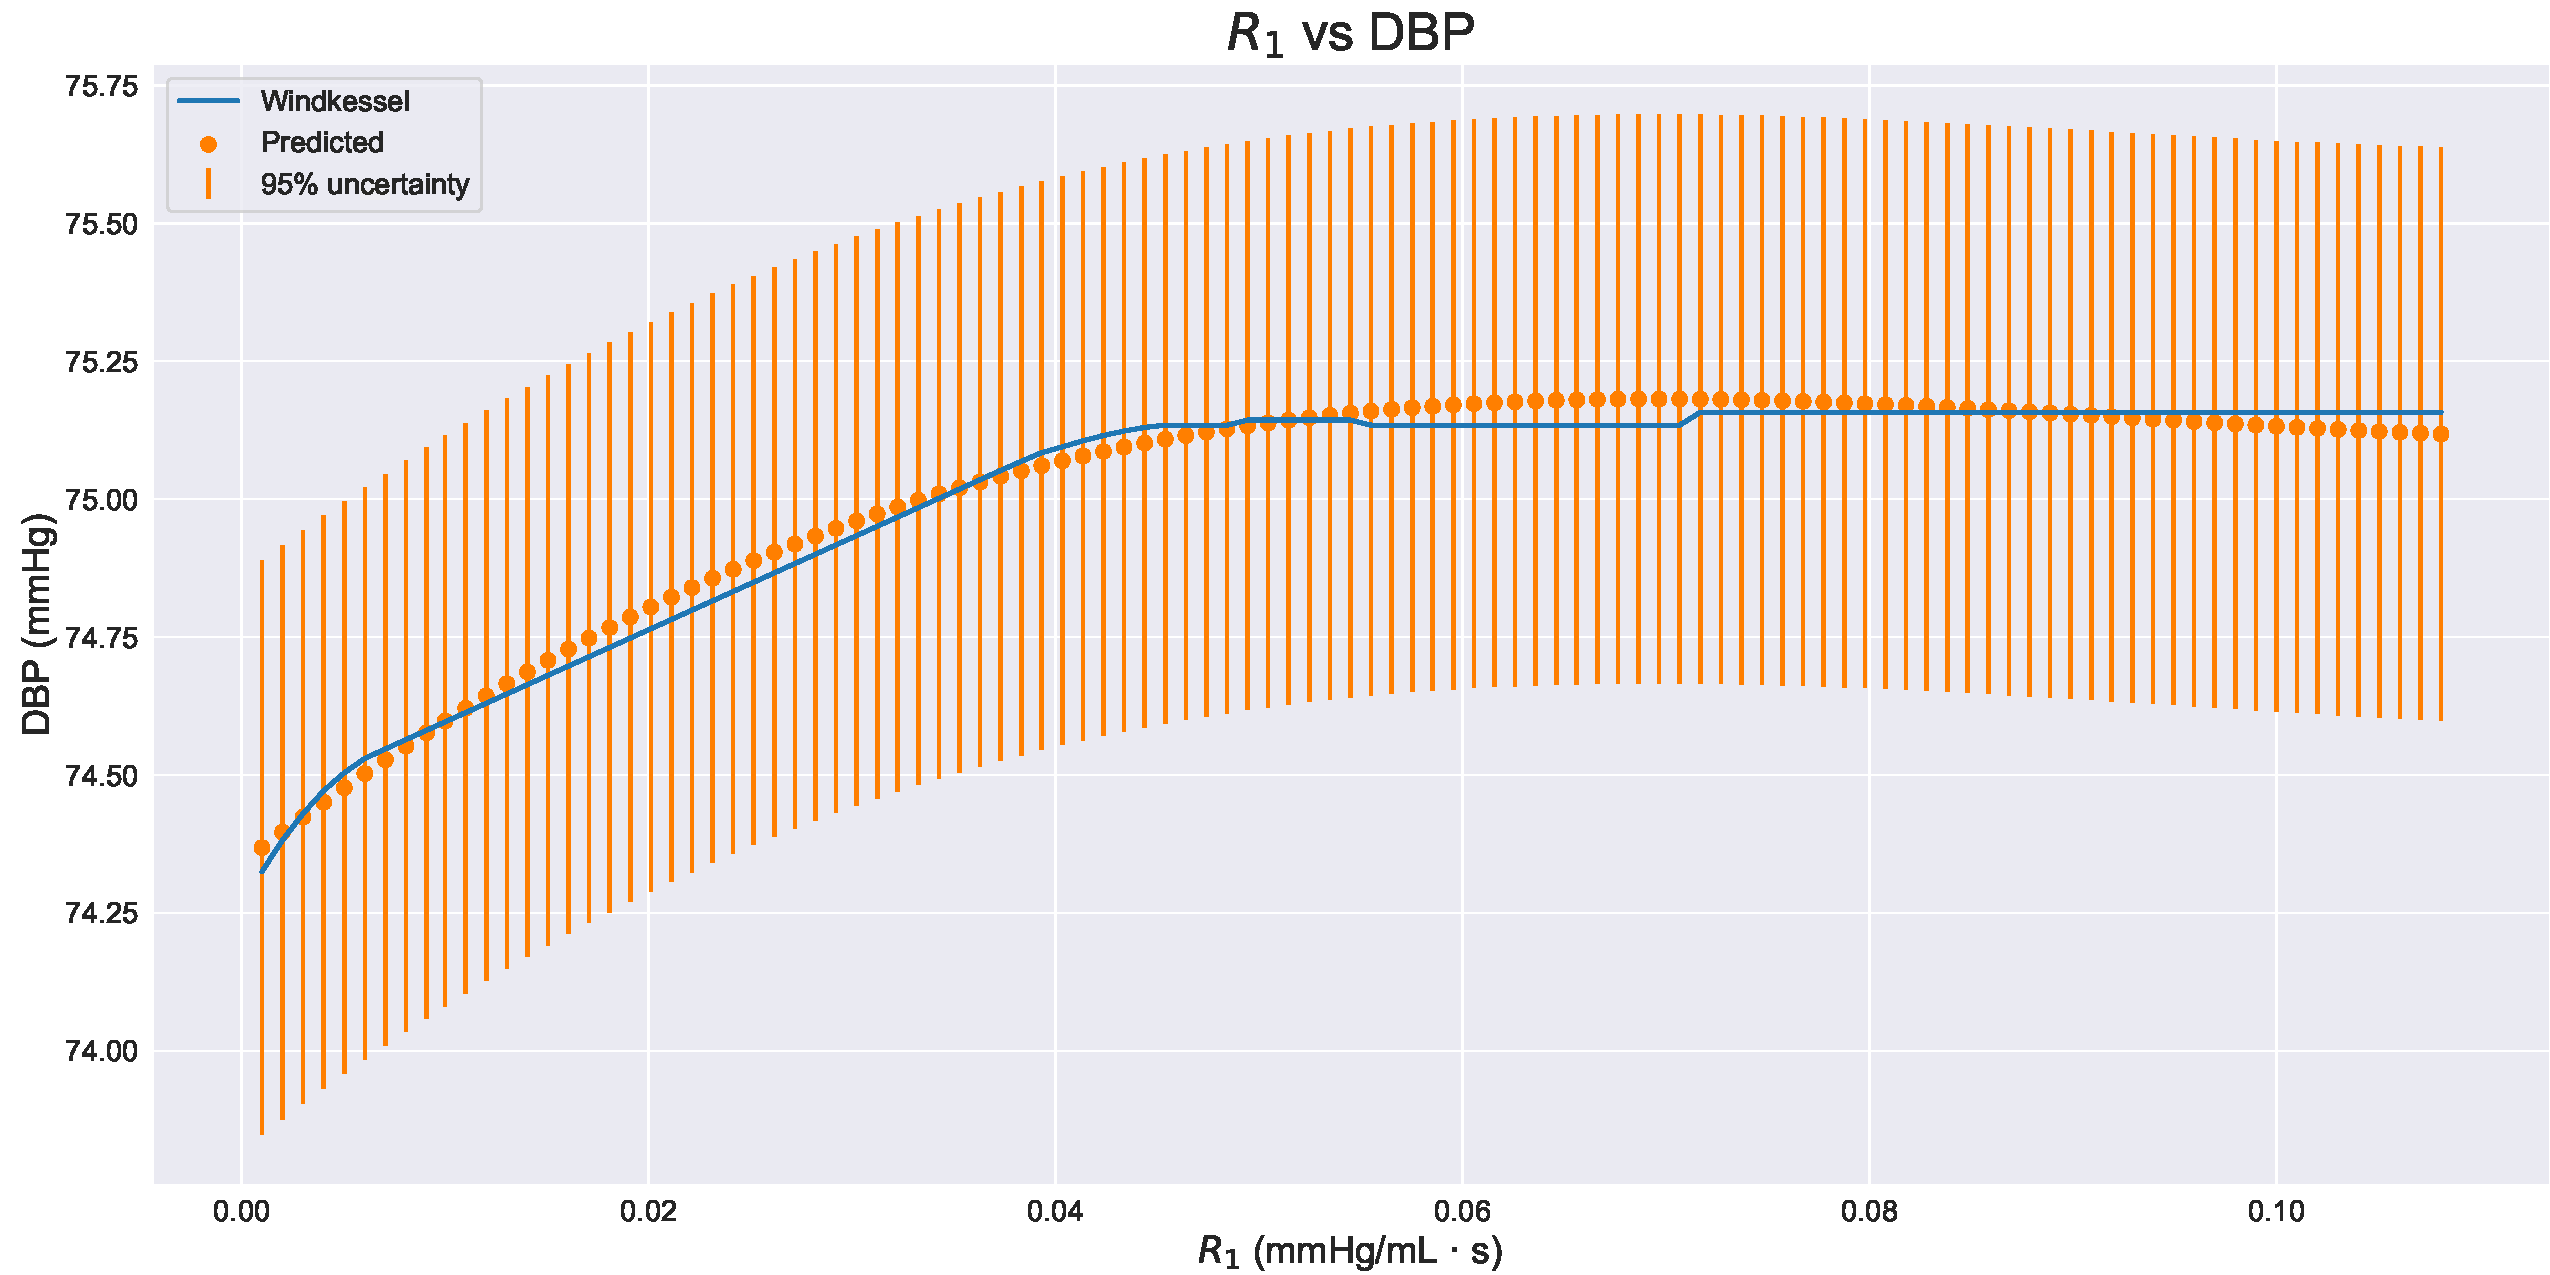
\includegraphics[width=1\textwidth]{images/Training (risultati)/DBP/DBP - R1 - full.pdf}
    \caption{Dependence of DBP on $R_1$ on the training interval and two adjacent intervals.}
    \label{DBP - R1 - full}
\end{figure}

\vspace{0.32cm}

\begin{figure}[!htb]
    \centering
    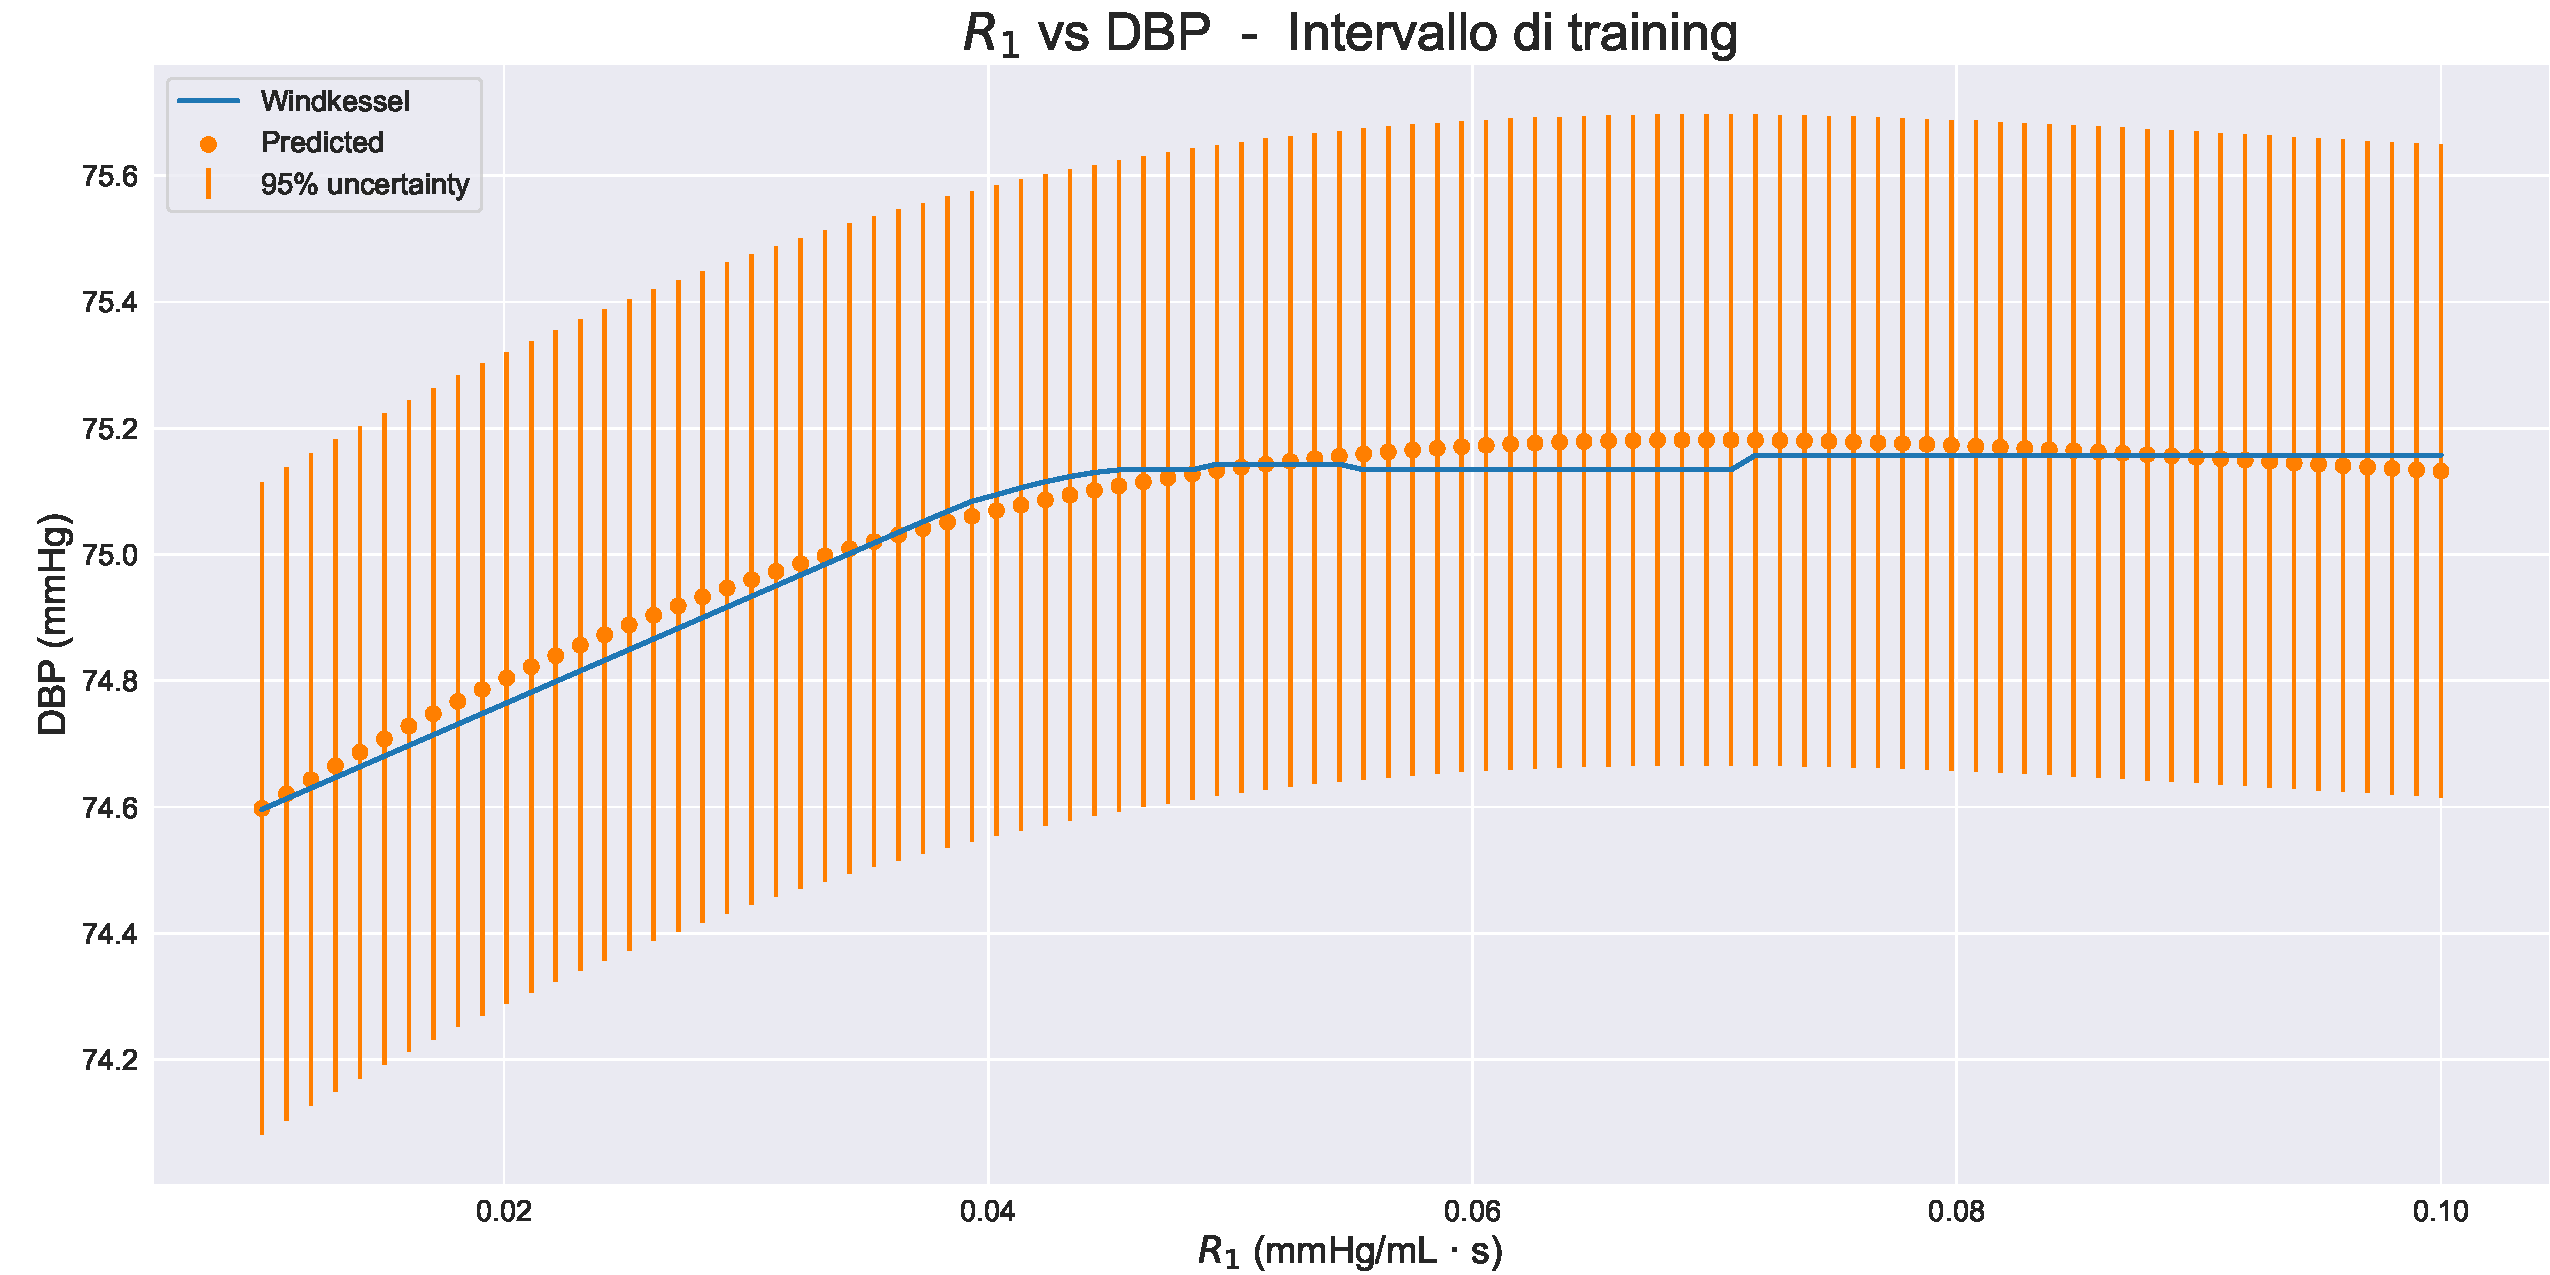
\includegraphics[width=1\textwidth]{images/Training (risultati)/DBP/DBP - R1 - training.pdf}
    \caption{Dependence of DBP on $R_1$ over the training interval.}
    \label{DBP - R1 - training}
\end{figure}

\begin{figure}
    \centering
    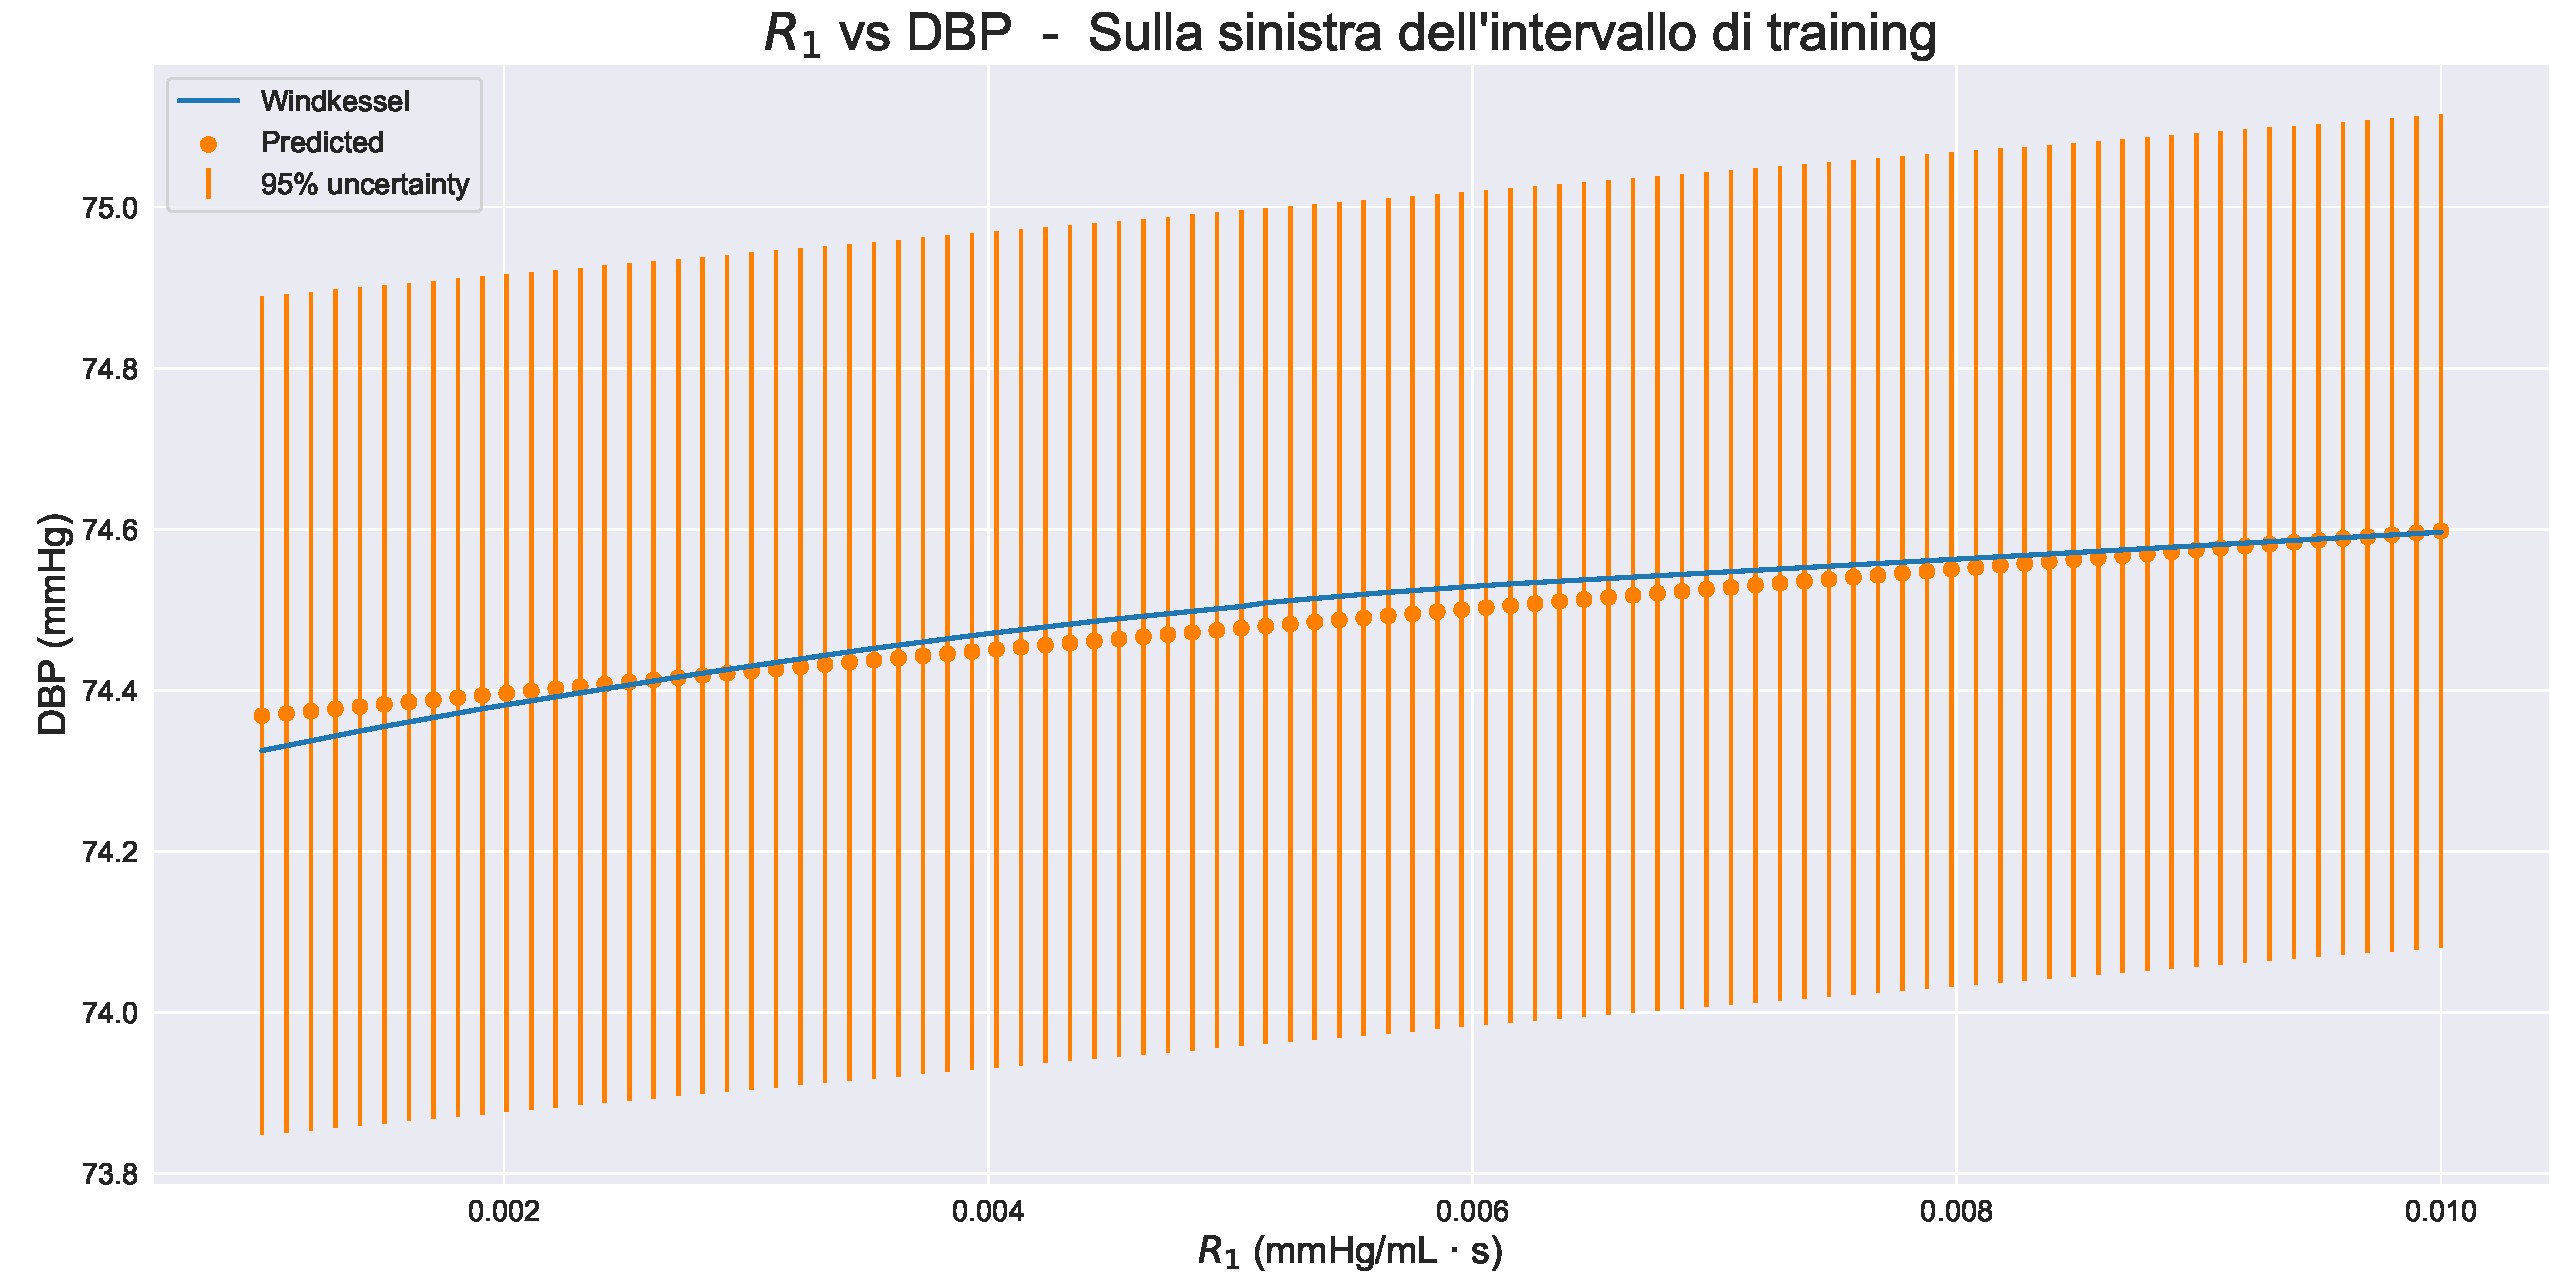
\includegraphics[width=1\textwidth]{images/Training (risultati)/DBP/DBP - R1 - sx.pdf}
    \caption{Dependence of DBP on $R_1$ on the adjoint interval to the left of the training interval.}
    \label{DBP - R1 - sx}
\end{figure}



\begin{figure}
    \centering
    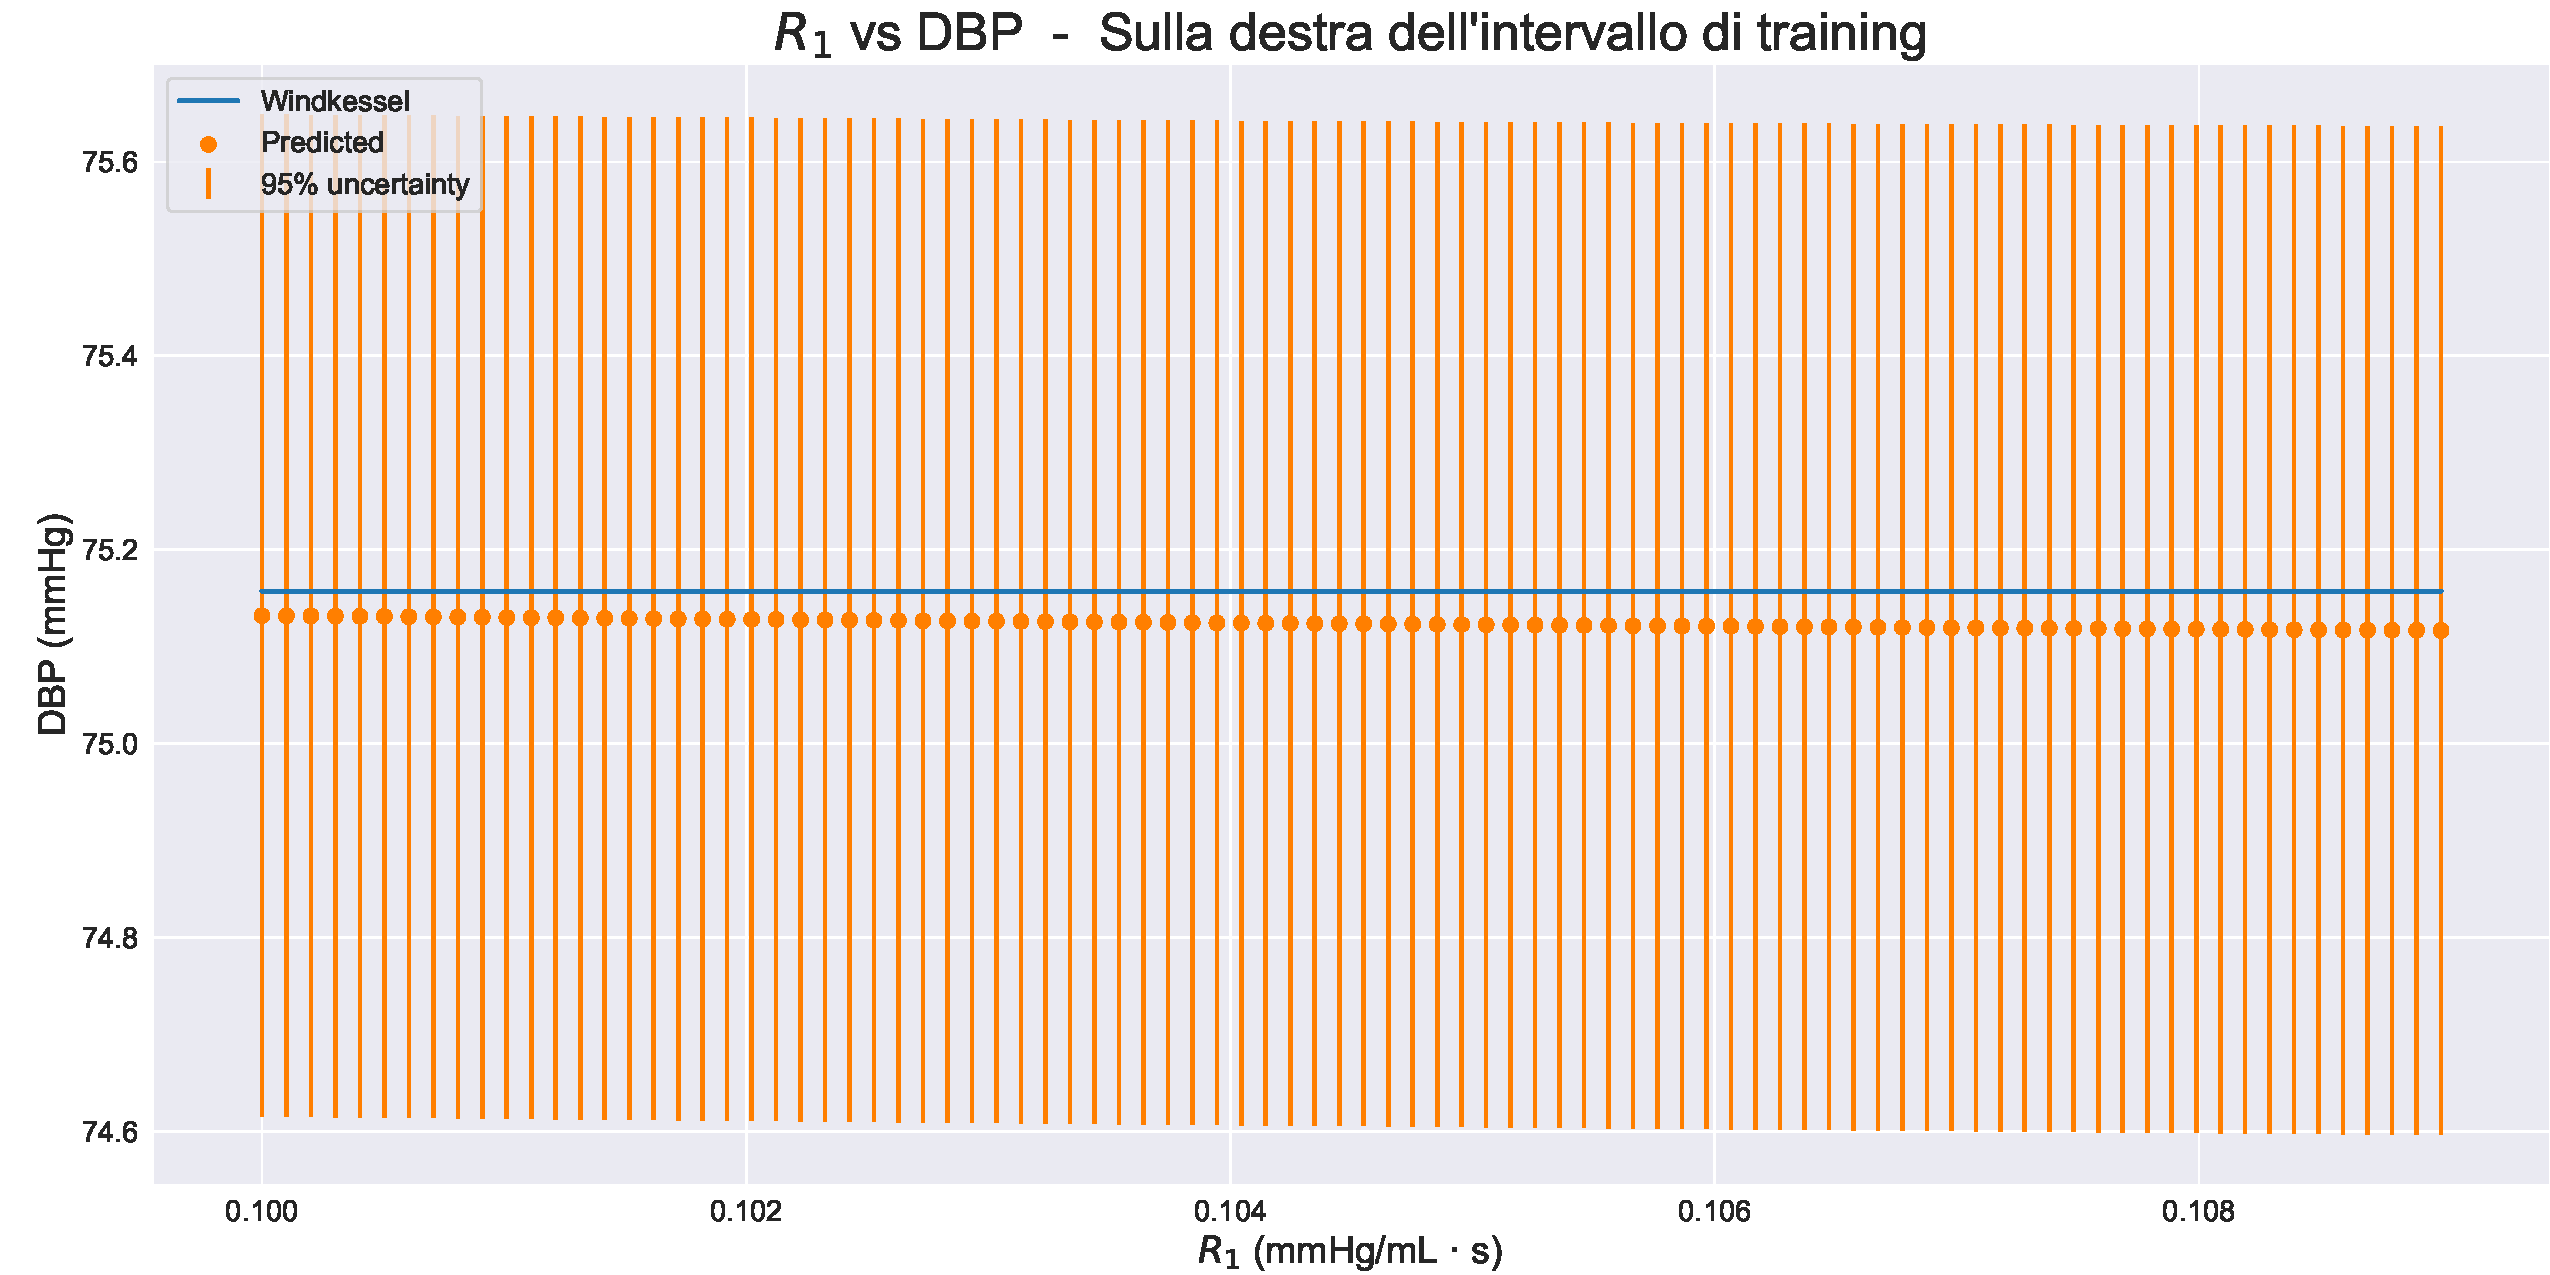
\includegraphics[width=1\textwidth]{images/Training (risultati)/DBP/DBP - R1 - dx.pdf}
    \caption{Dependence of DBP on $R_1$ on the adjoint interval to the right of the training interval.}
    \label{DBP - R1 - dx}
\end{figure}



\newpage
% **********
% DBP - R2
% **********
\subsubsection{Dependence on $R_2$}
The overall result is shown in figure \ref{DBP - R2 - full}, the result in the training interval alone in \ref{DBP - R2 - training}, the result in the individual adjacent intervals in \ref{DBP - R2 - sx} and \ref{DBP - R2 - dx}. Again there are very accurate predictions. At first glance it appears that the error bars do not appear; in fact they are very short compared to the scale used. In fact, in graphs where only the adjacent intervals are plotted the error bars reappear and show that the error is less than one unit.

\vspace{1cm}

\begin{figure}[!htb]
    \centering
    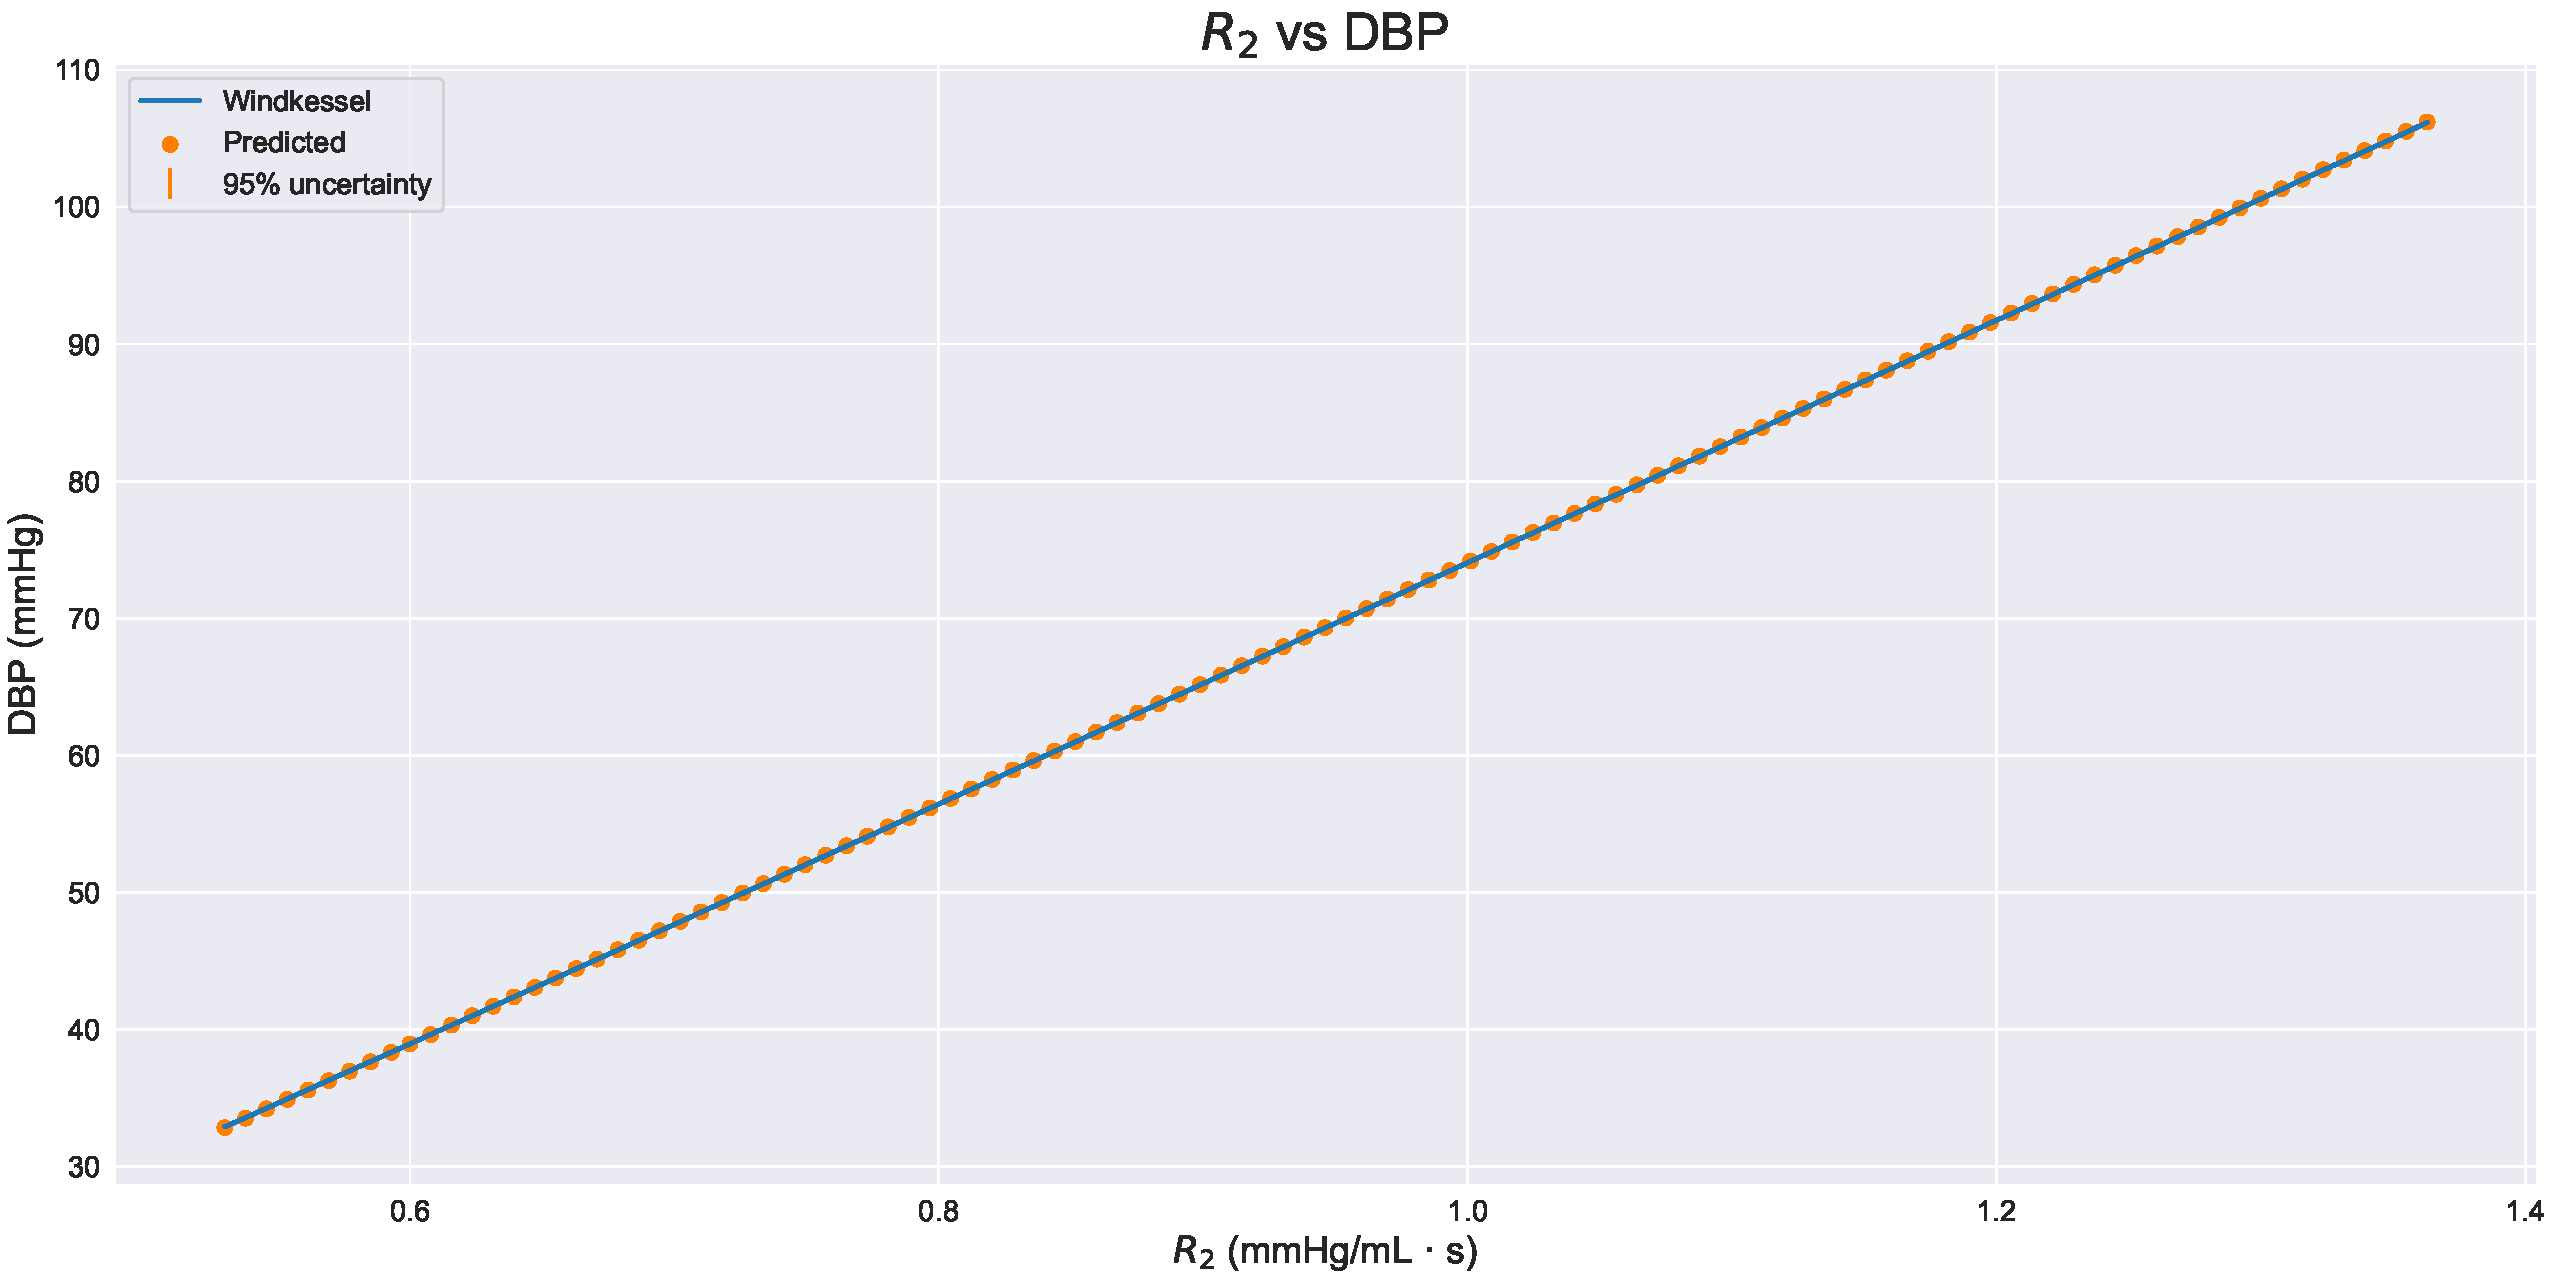
\includegraphics[width=1\textwidth]{images/Training (risultati)/DBP/DBP - R2 - full.pdf}
    \caption{Dependence of DBP on $R_2$ on the training interval and two adjacent intervals.}
    \label{DBP - R2 - full}
\end{figure}

\vspace{0.34cm}

\begin{figure}[!htb]
    \centering
    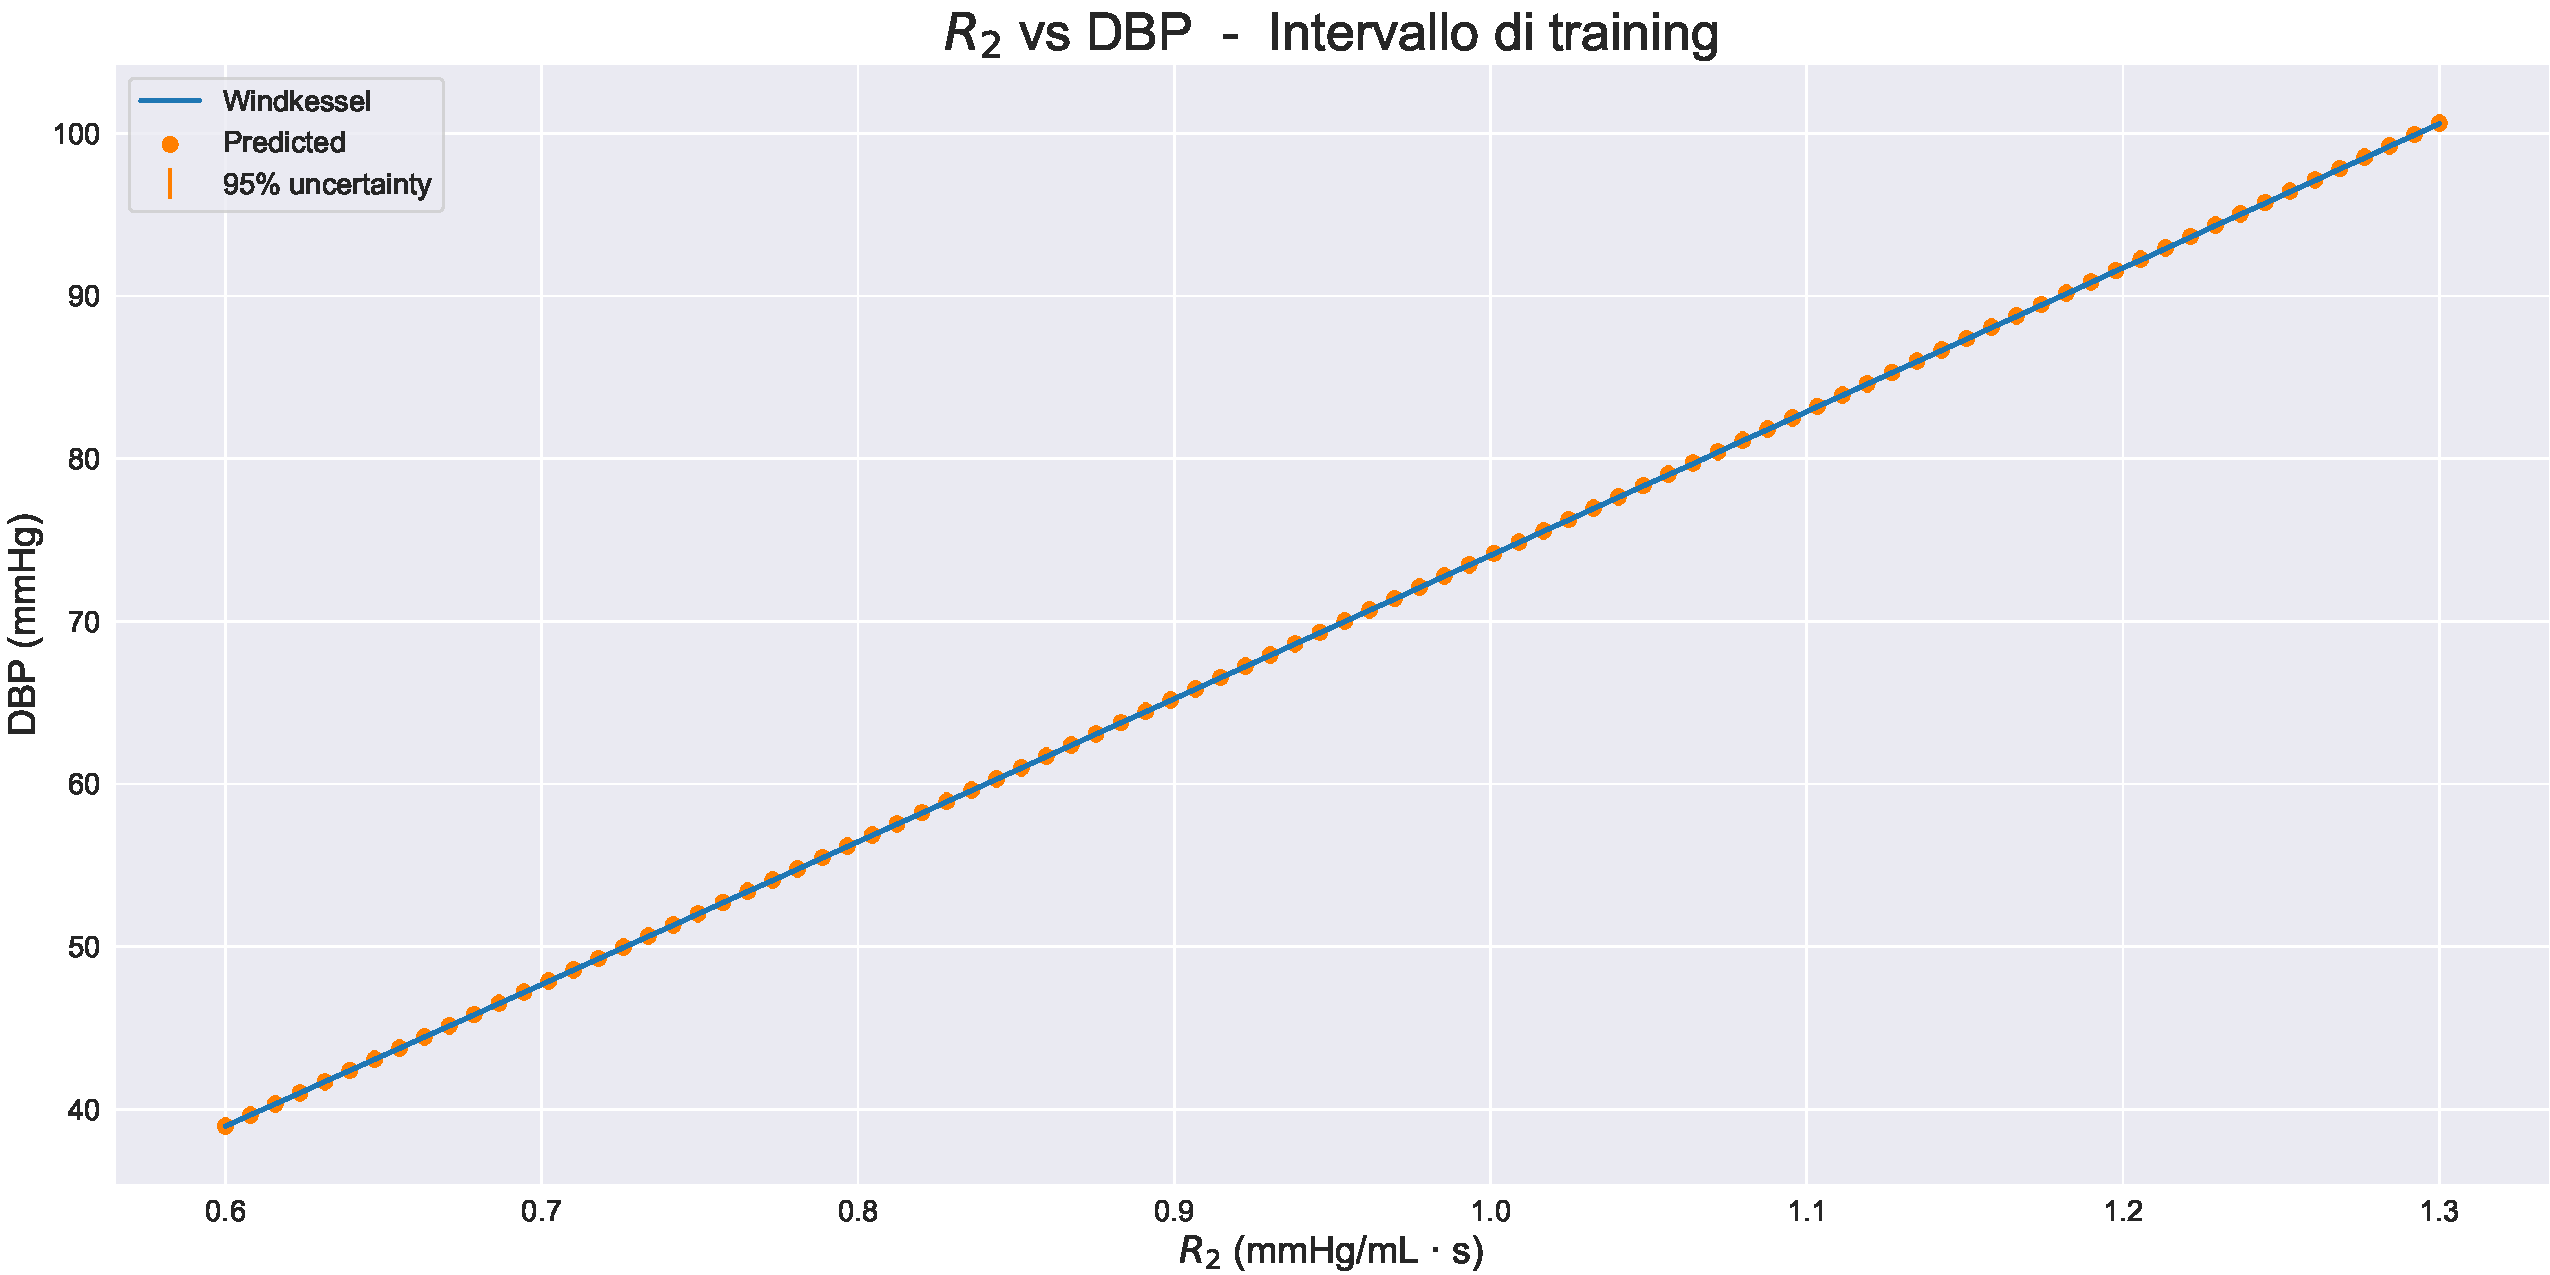
\includegraphics[width=1\textwidth]{images/Training (risultati)/DBP/DBP - R2 - training.pdf}
    \caption{Dependence of DBP on $R_2$ over the training interval.}
    \label{DBP - R2 - training}
\end{figure}

\begin{figure}
    \centering
    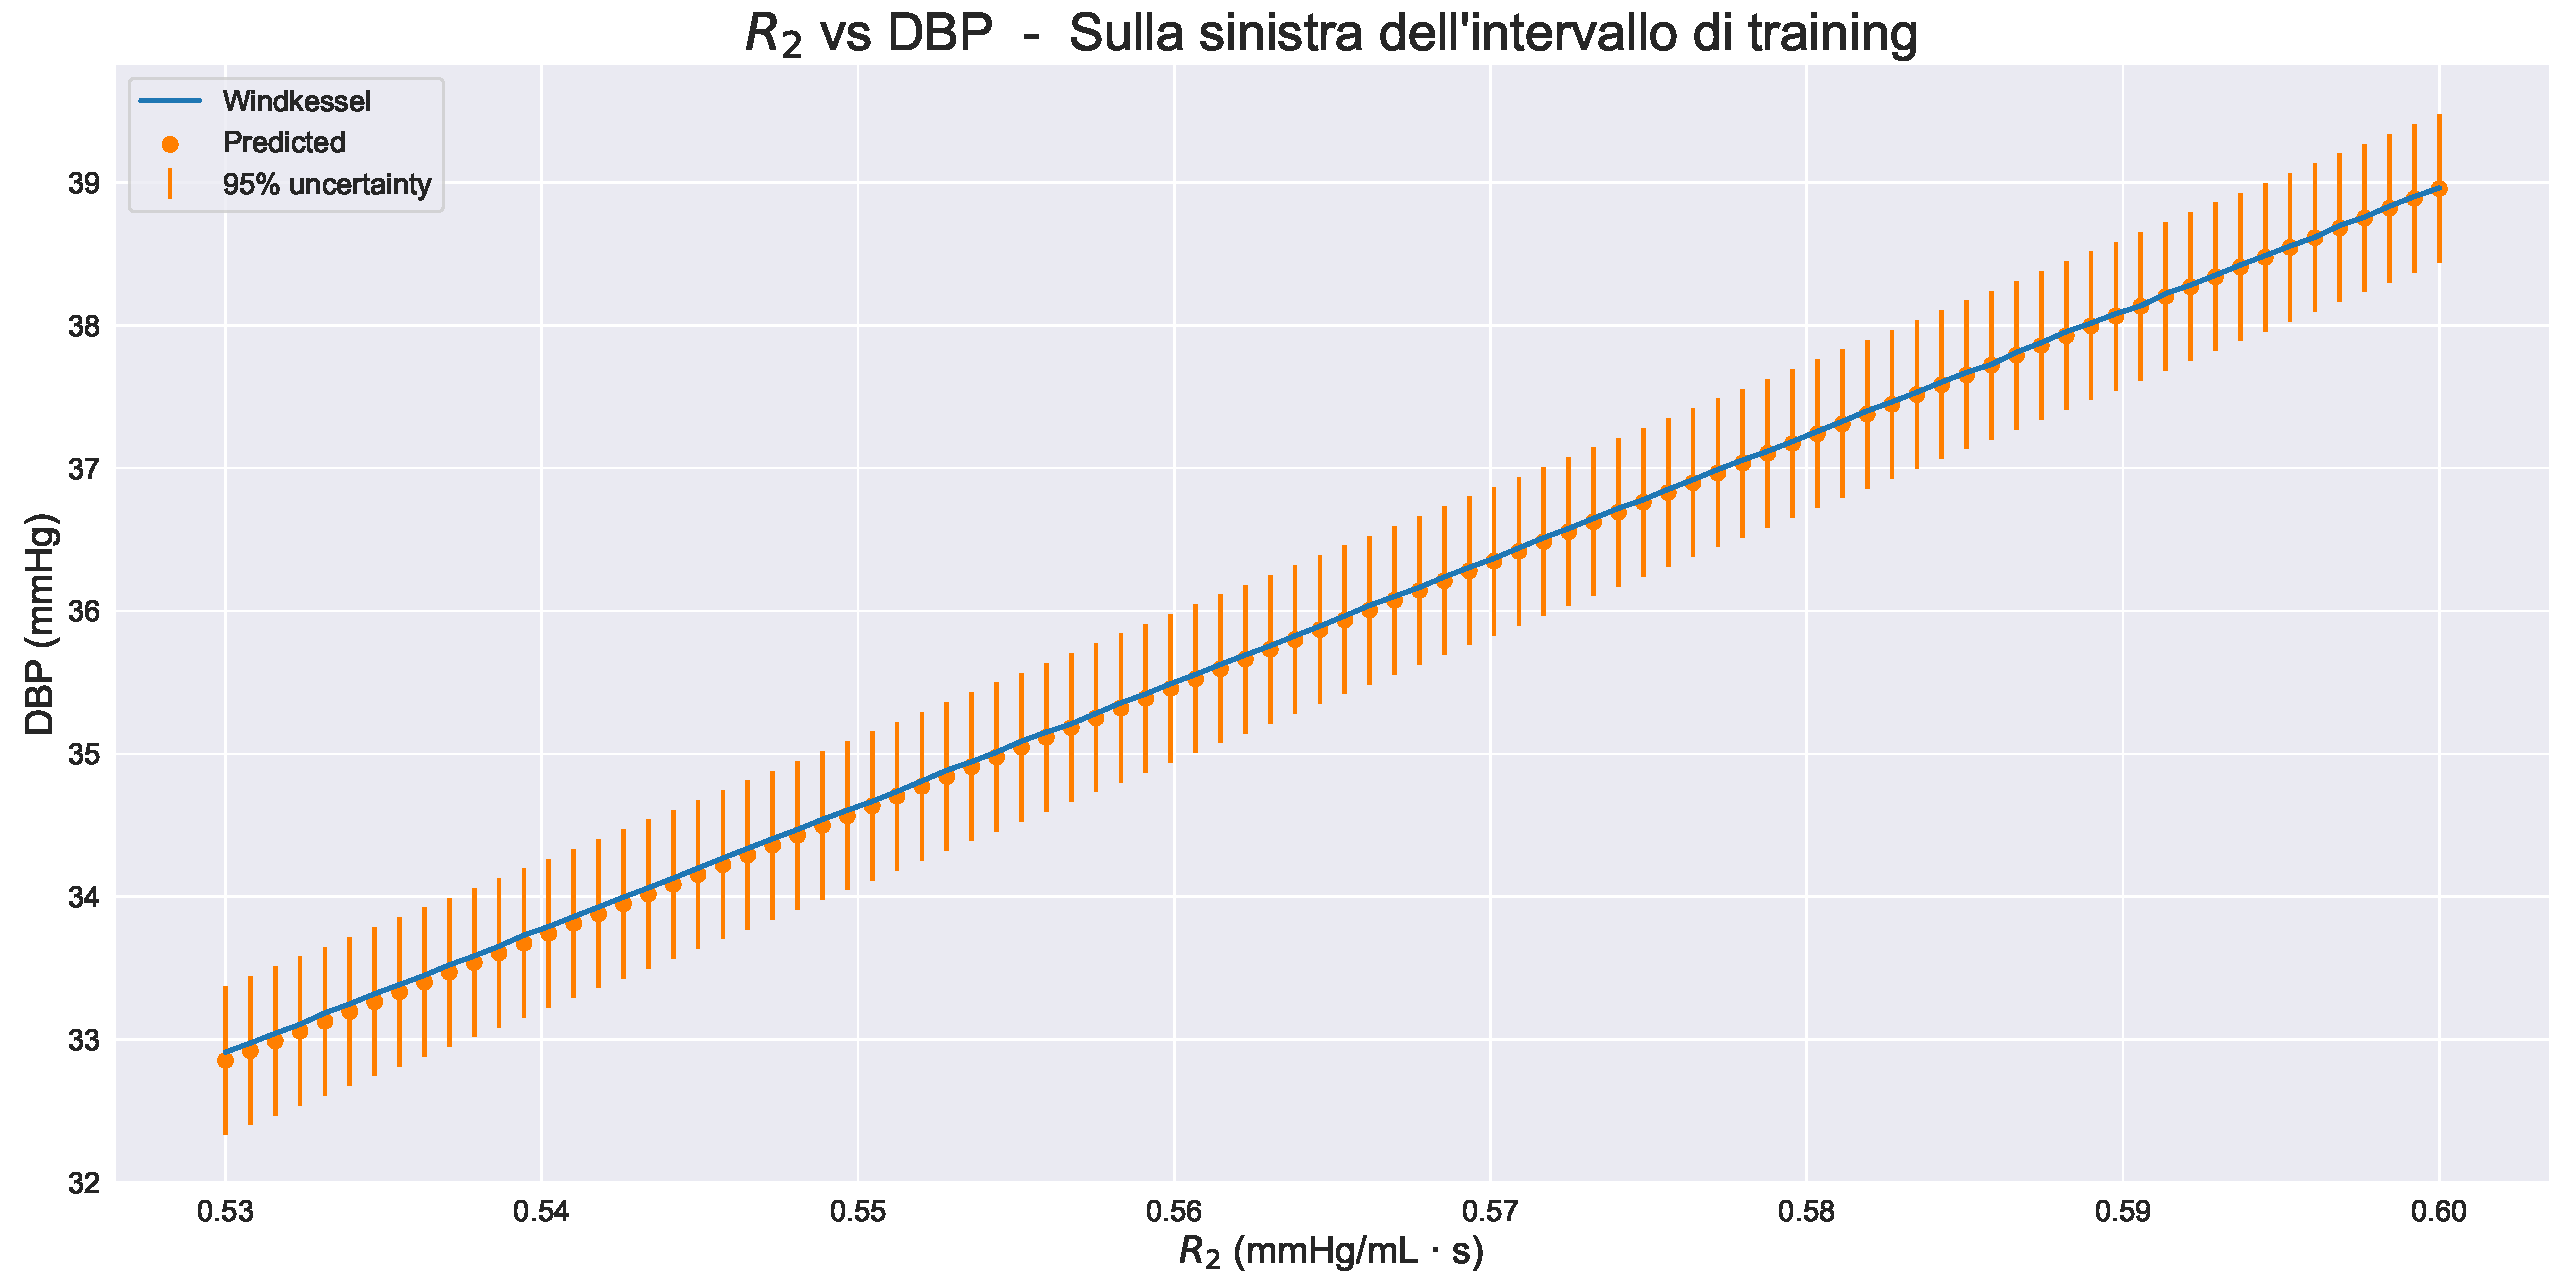
\includegraphics[width=1\textwidth]{images/Training (risultati)/DBP/DBP - R2 - sx.pdf}
    \caption{Dependence of DBP on $R_2$ on the adjoint interval to the left of the training interval.}
    \label{DBP - R2 - sx}
\end{figure}


\begin{figure}
    \centering
    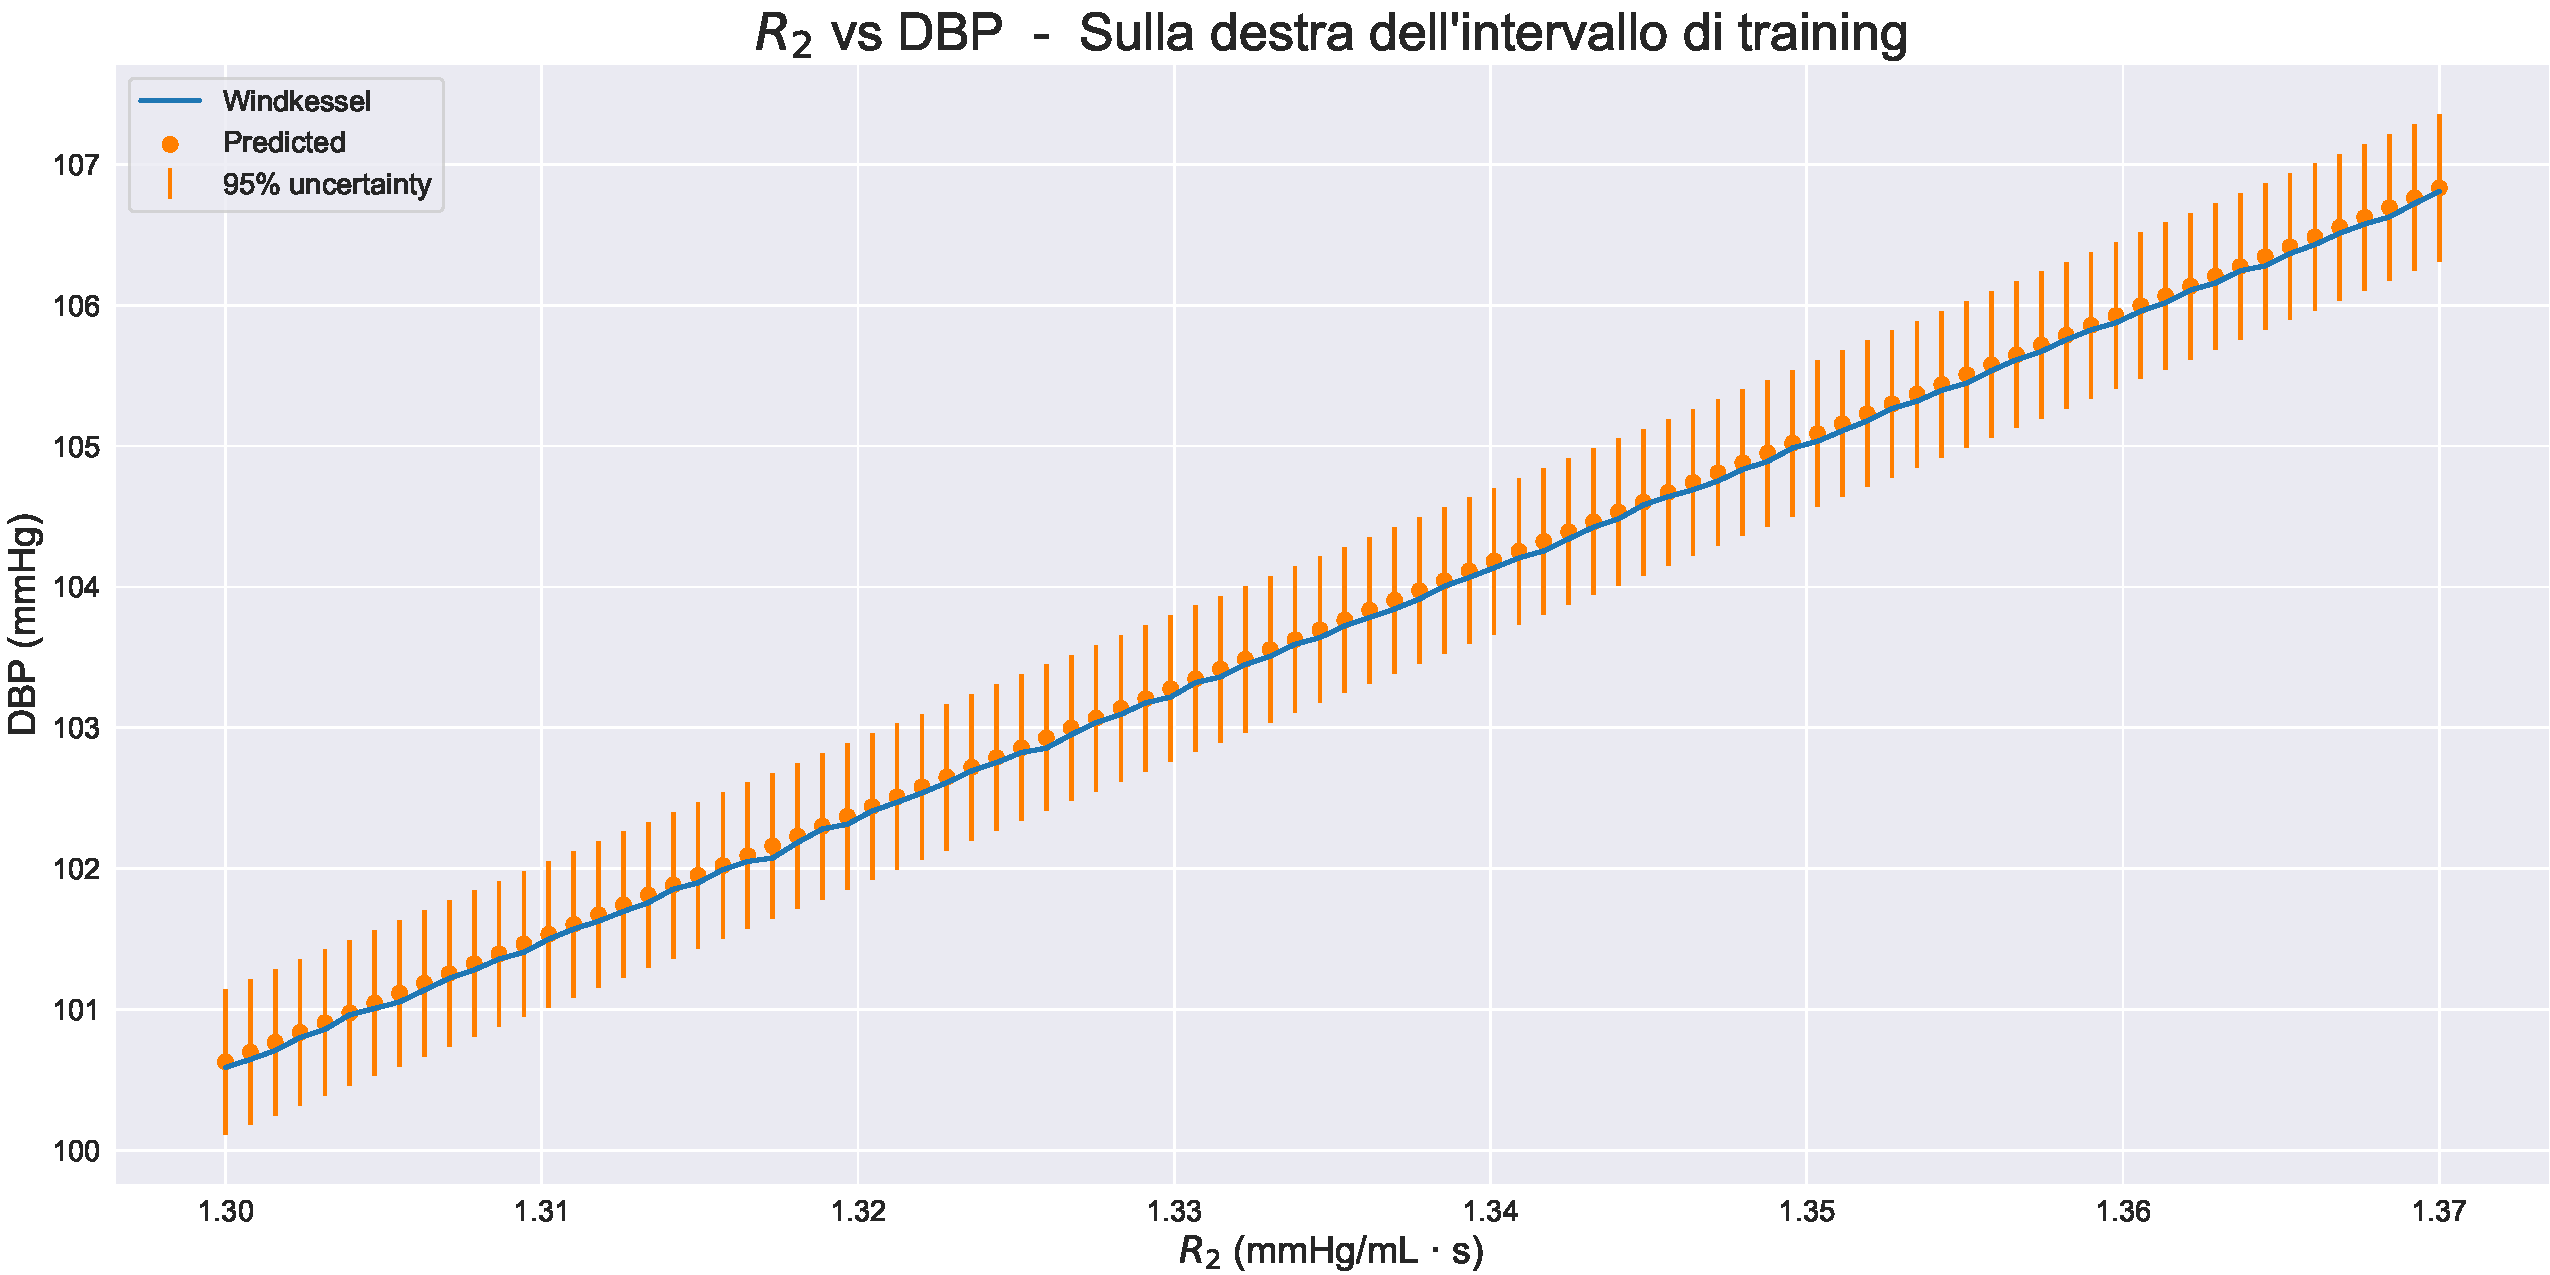
\includegraphics[width=1\textwidth]{images/Training (risultati)/DBP/DBP - R2 - dx.pdf}
    \caption{Dependence of DBP on $R_2$ on the adjoint interval to the right of the training interval.}
    \label{DBP - R2 - dx}
\end{figure}







\newpage
%******************************
%*********** PP **************
%******************************
\subsection{Pulse pressure (PP)}
$\text{lr}=0.05$ is imposed and the early stopper \textit{GLEarlyStoppingCriterion} is used with parameters: $\alpha = 5$, $\text{patience}=3$.


% **********
% PP - loss
% **********
\subsubsection{Training and validation loss}
The training needed ninety-three EPOCHS, concluded with $\text{R2Score}=0.9994$, $\text{MeanSquaredError}=0.0006$. Figure \ref{PP - loss} shows the training and validation loss trend with MSE and R2Score; early stopper trend in green.
\begin{figure}[h]
    \centering
    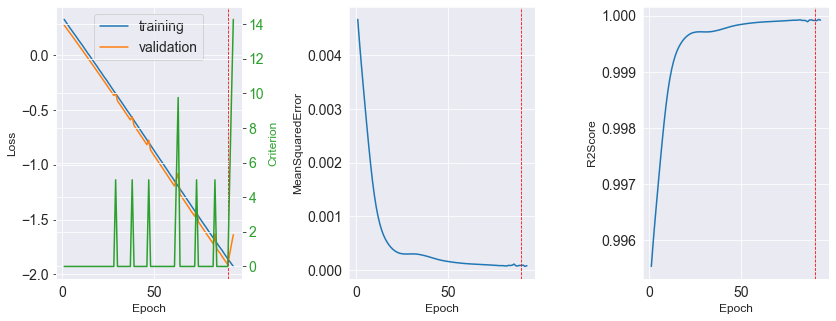
\includegraphics[width=1\textwidth]{images/Training (risultati)/PP/PP - loss.png}
    \caption{PP: progress of training and validation loss, early stopper, R2Score and MSE.}
    \label{PP - loss}
\end{figure}

\vspace{-0.5cm}

% **********
% PP - inference
% **********
\subsubsection{Approximation of input data}
Figure \ref{PP - inference} shows how the predictions approximate the input data. The length of the error bars is $0.0034$.

\begin{figure}[h]
    \centering
    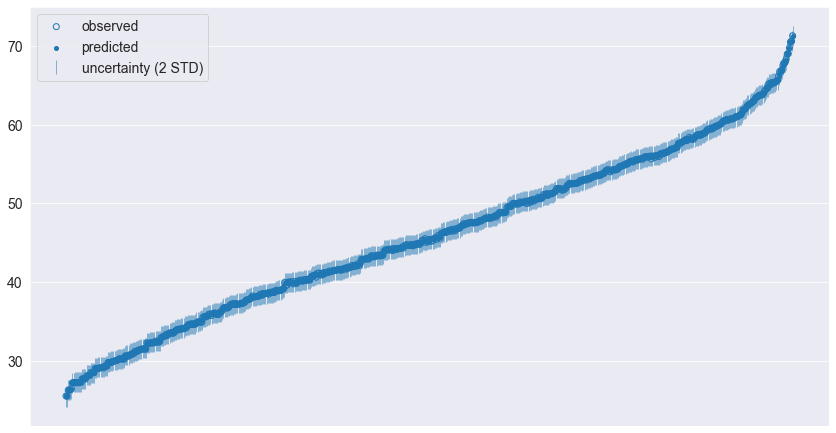
\includegraphics[width=1\textwidth]{images/Training (risultati)/PP/PP - inference.png}
    \caption{PP: predictions about the input data.}
    \label{PP - inference}
\end{figure}



% **********
% PP - C
% **********
\subsubsection{Dependence on $C$}
The overall result is shown in figure \ref{PP - C - full}, the result in the training interval alone in \ref{PP - C - training}, the result in the individual adjacent intervals in \ref{PP - C - sx} and \ref{PP - C - dx}.

\vspace{1cm}

\begin{figure}[!htb]
    \centering
    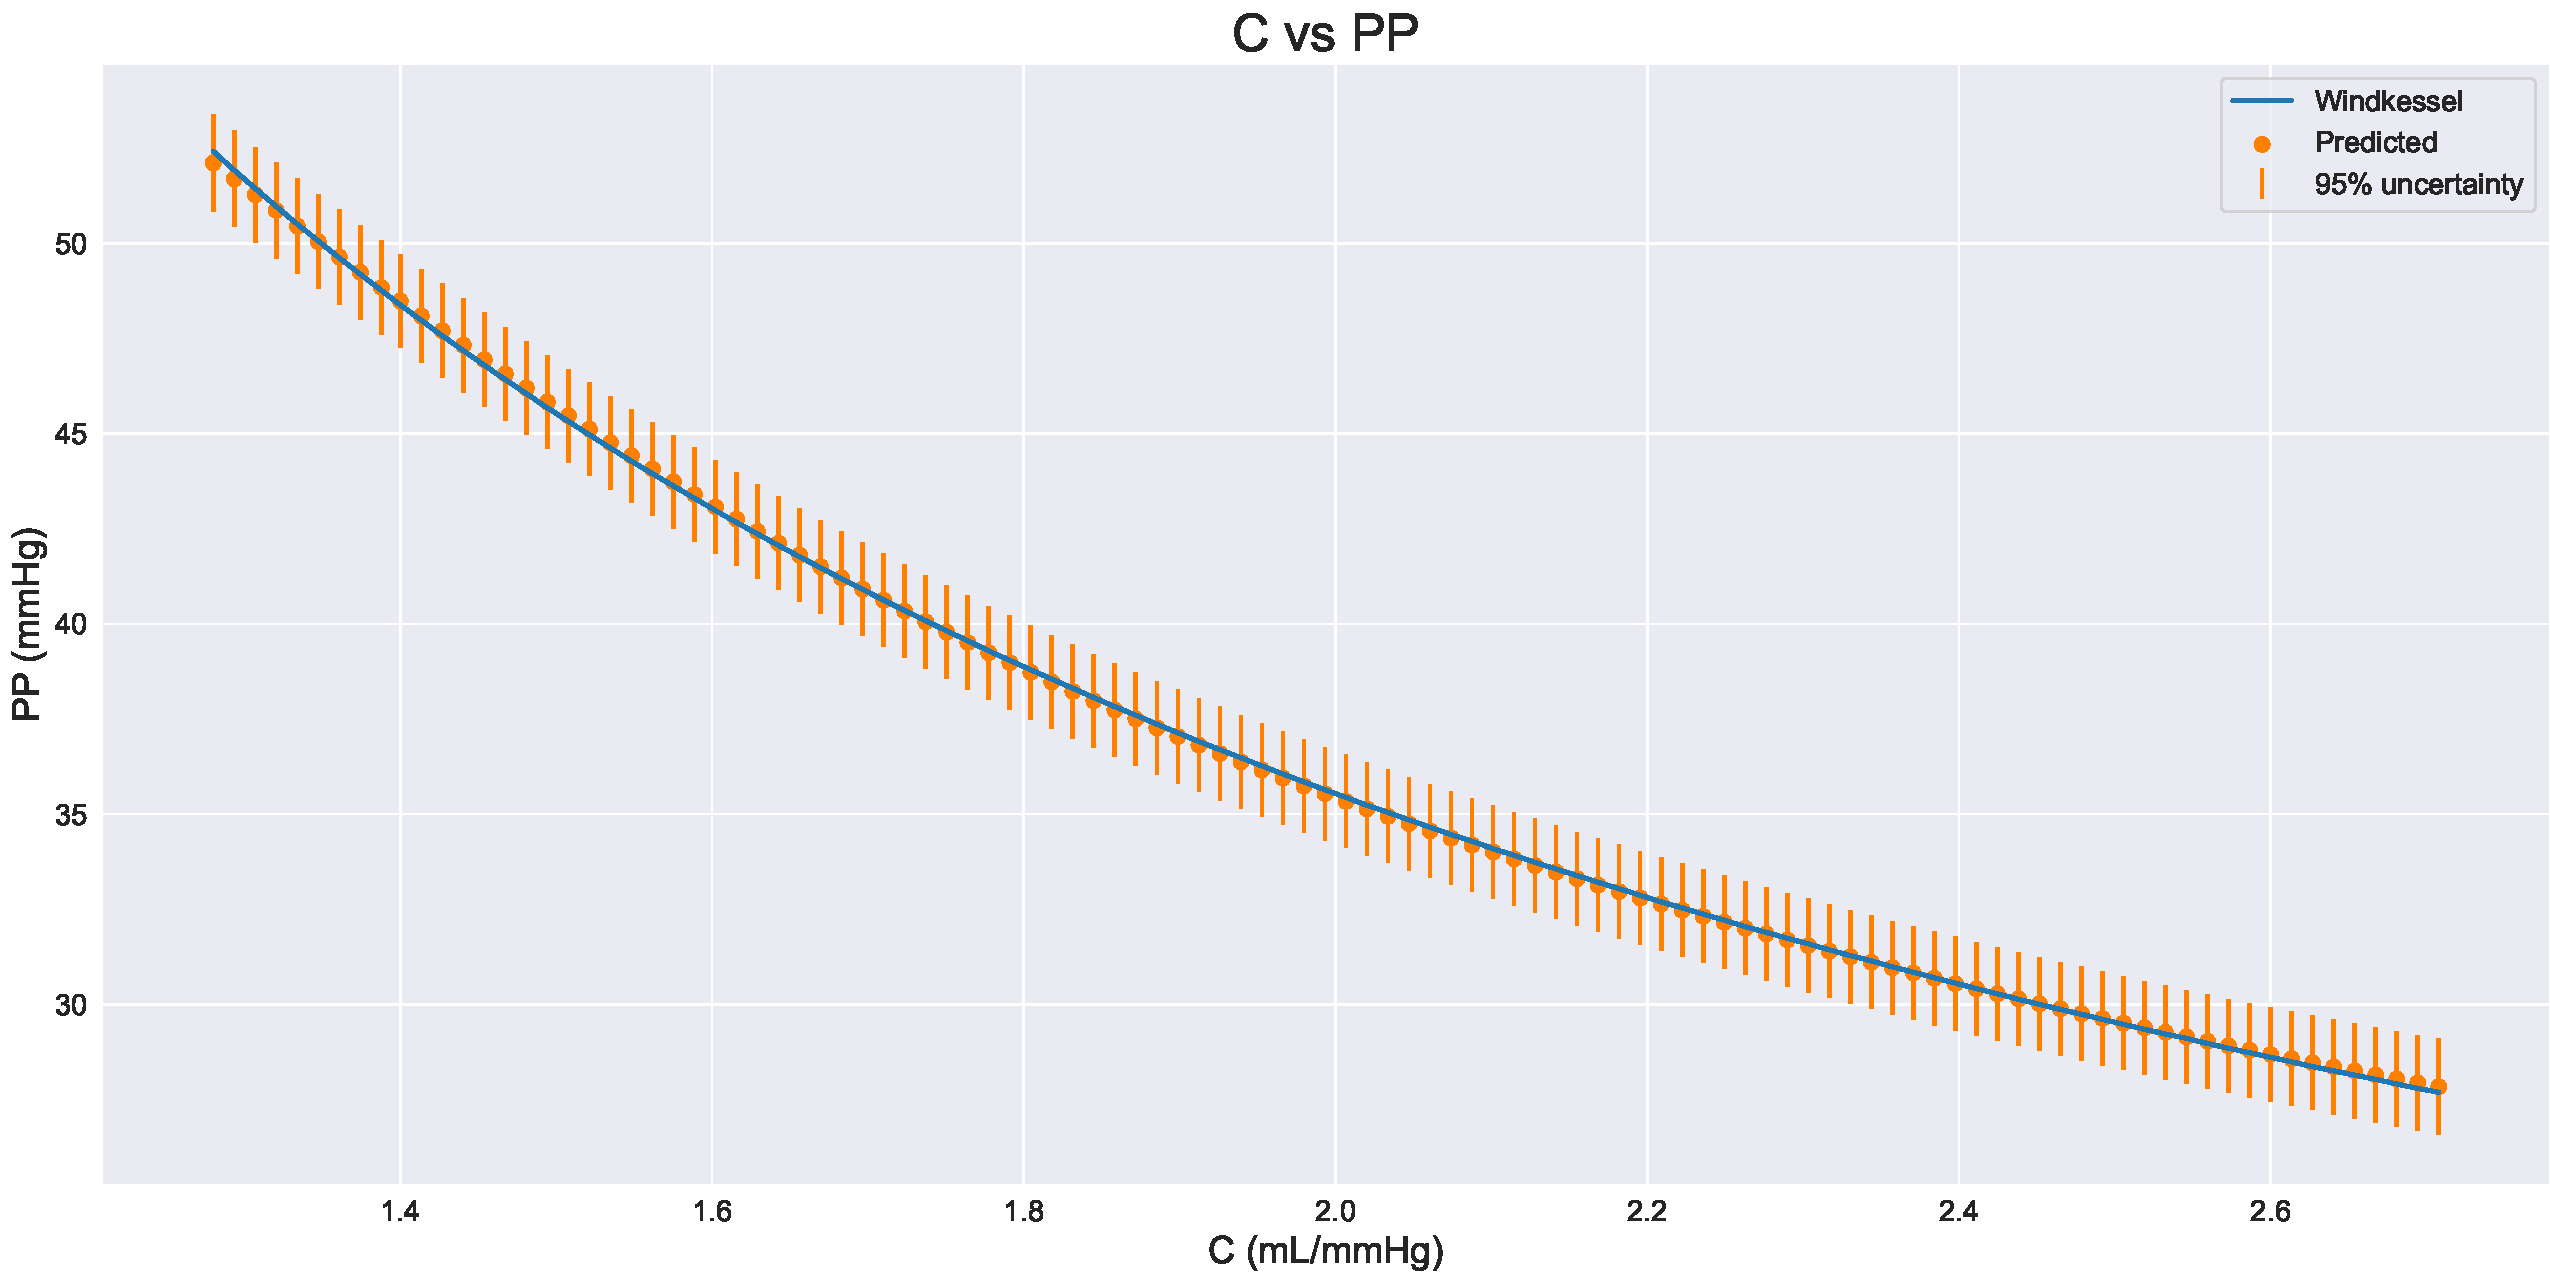
\includegraphics[width=1\textwidth]{images/Training (risultati)/PP/PP - C - full.pdf}
    \caption{Dependence of PP on $C$ on the training interval and two adjacent intervals.}
    \label{PP - C - full}
\end{figure}

\vspace{0.32cm}

\begin{figure}[!htb]
    \centering
    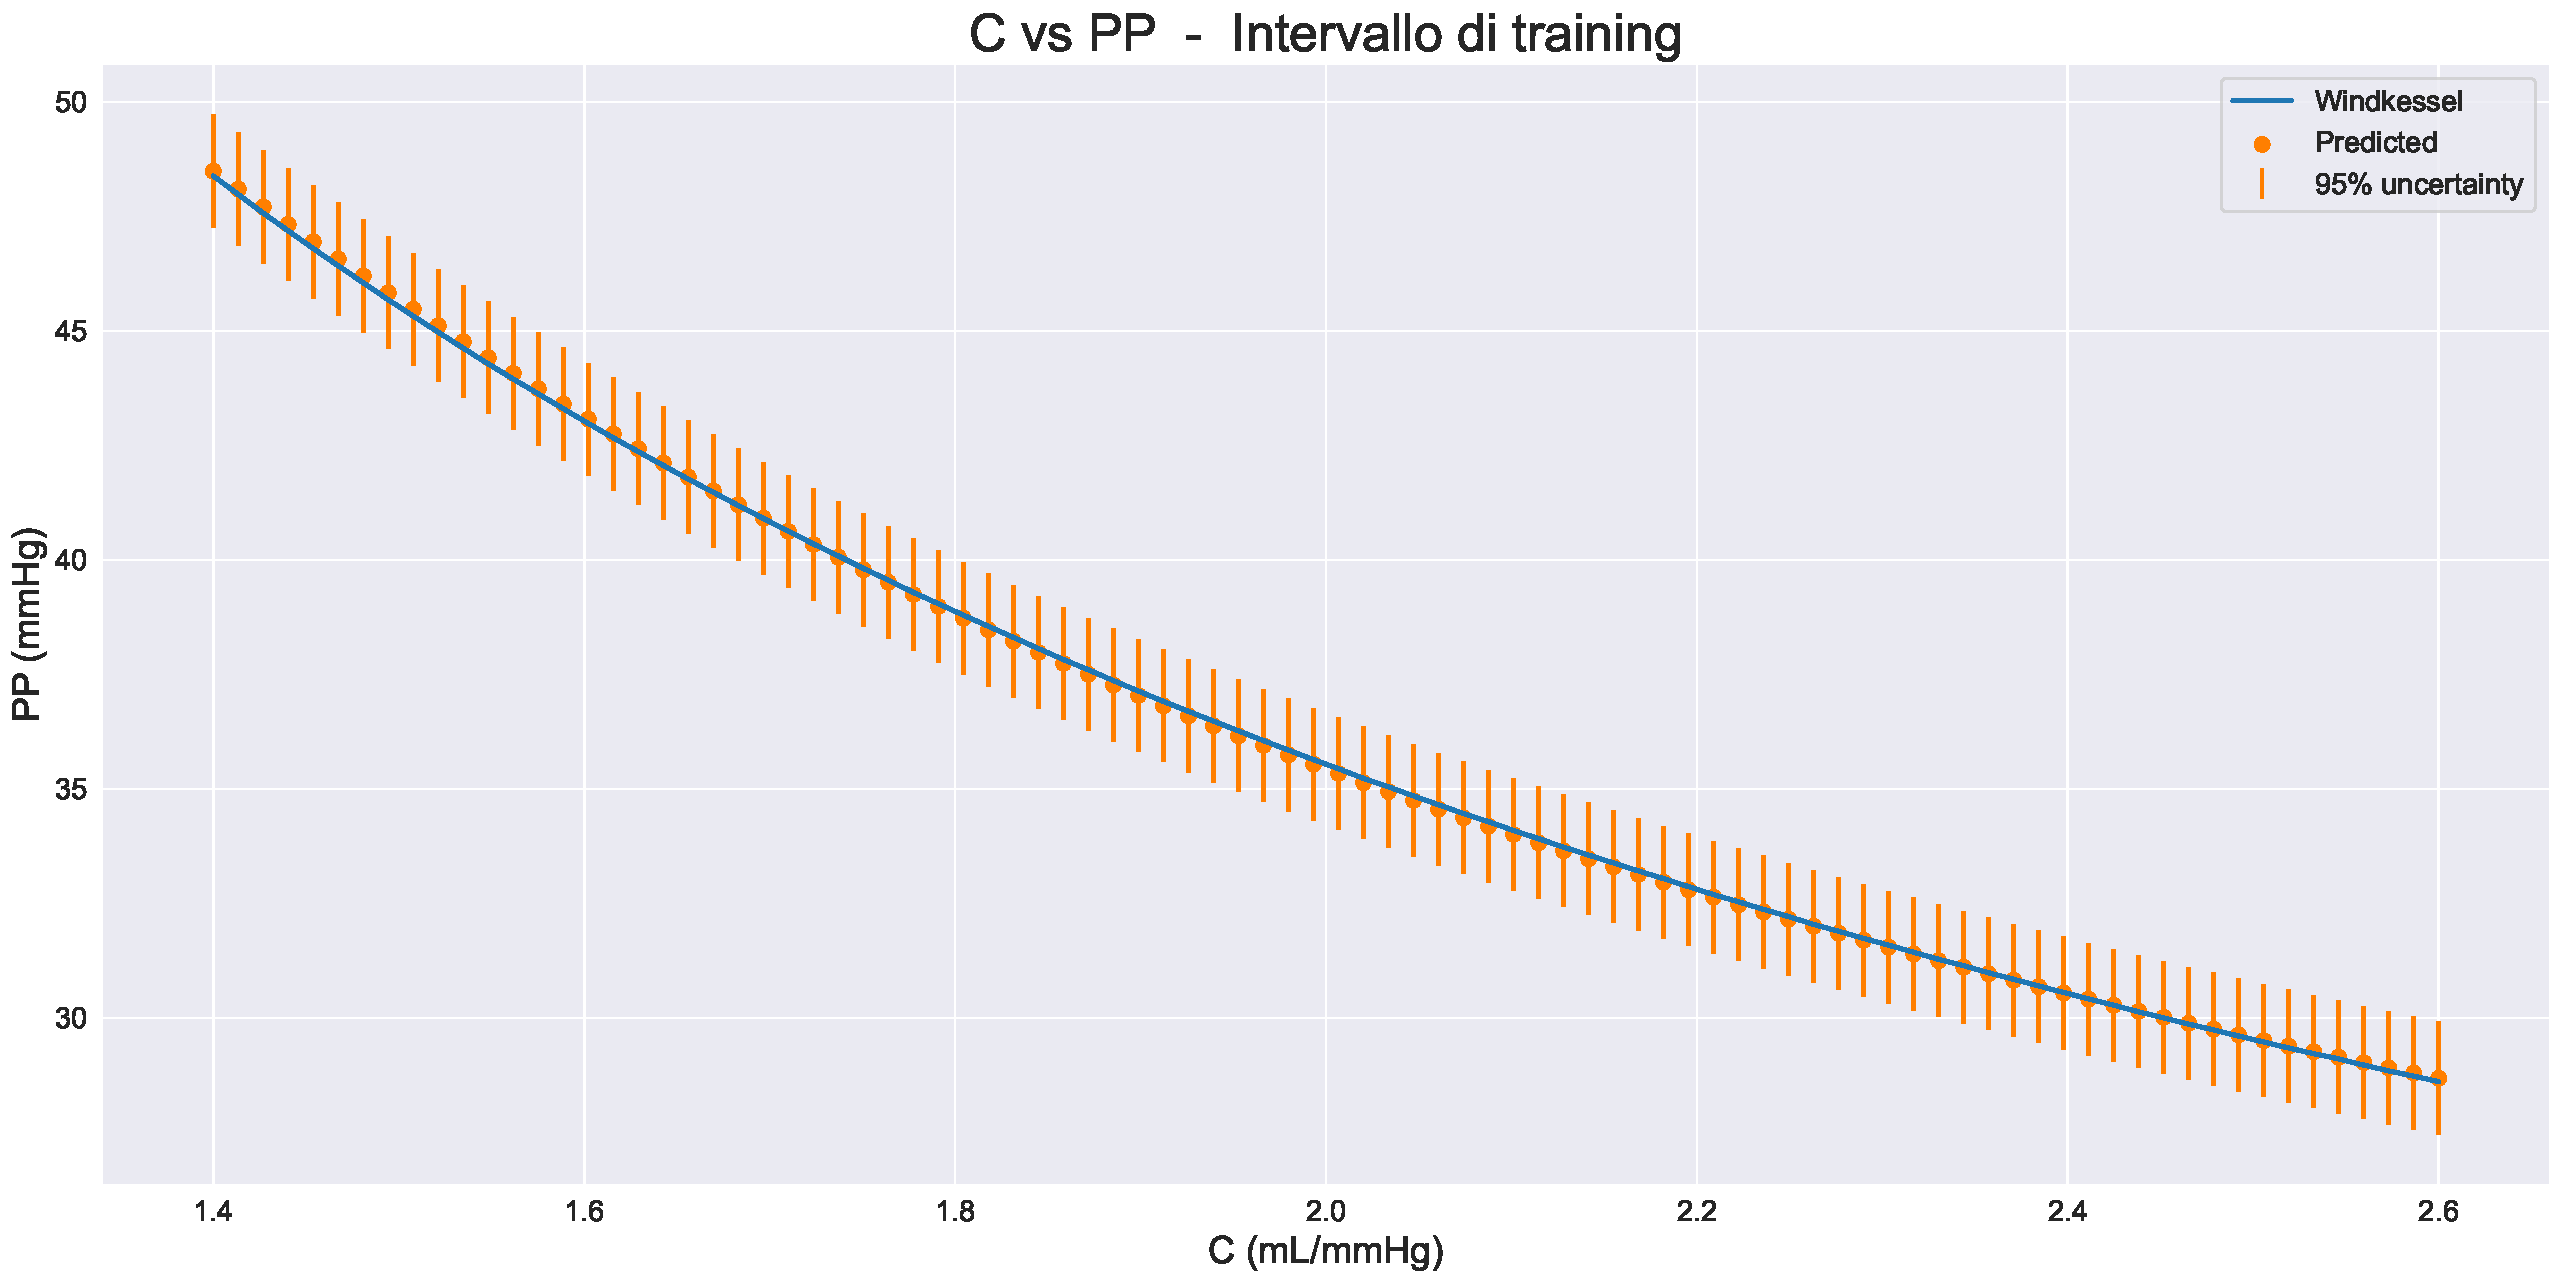
\includegraphics[width=1\textwidth]{images/Training (risultati)/PP/PP - C - training.pdf}
    \caption{Dependence of PP on $C$ over the training interval.}
    \label{PP - C - training}
\end{figure}

\begin{figure}
    \centering
    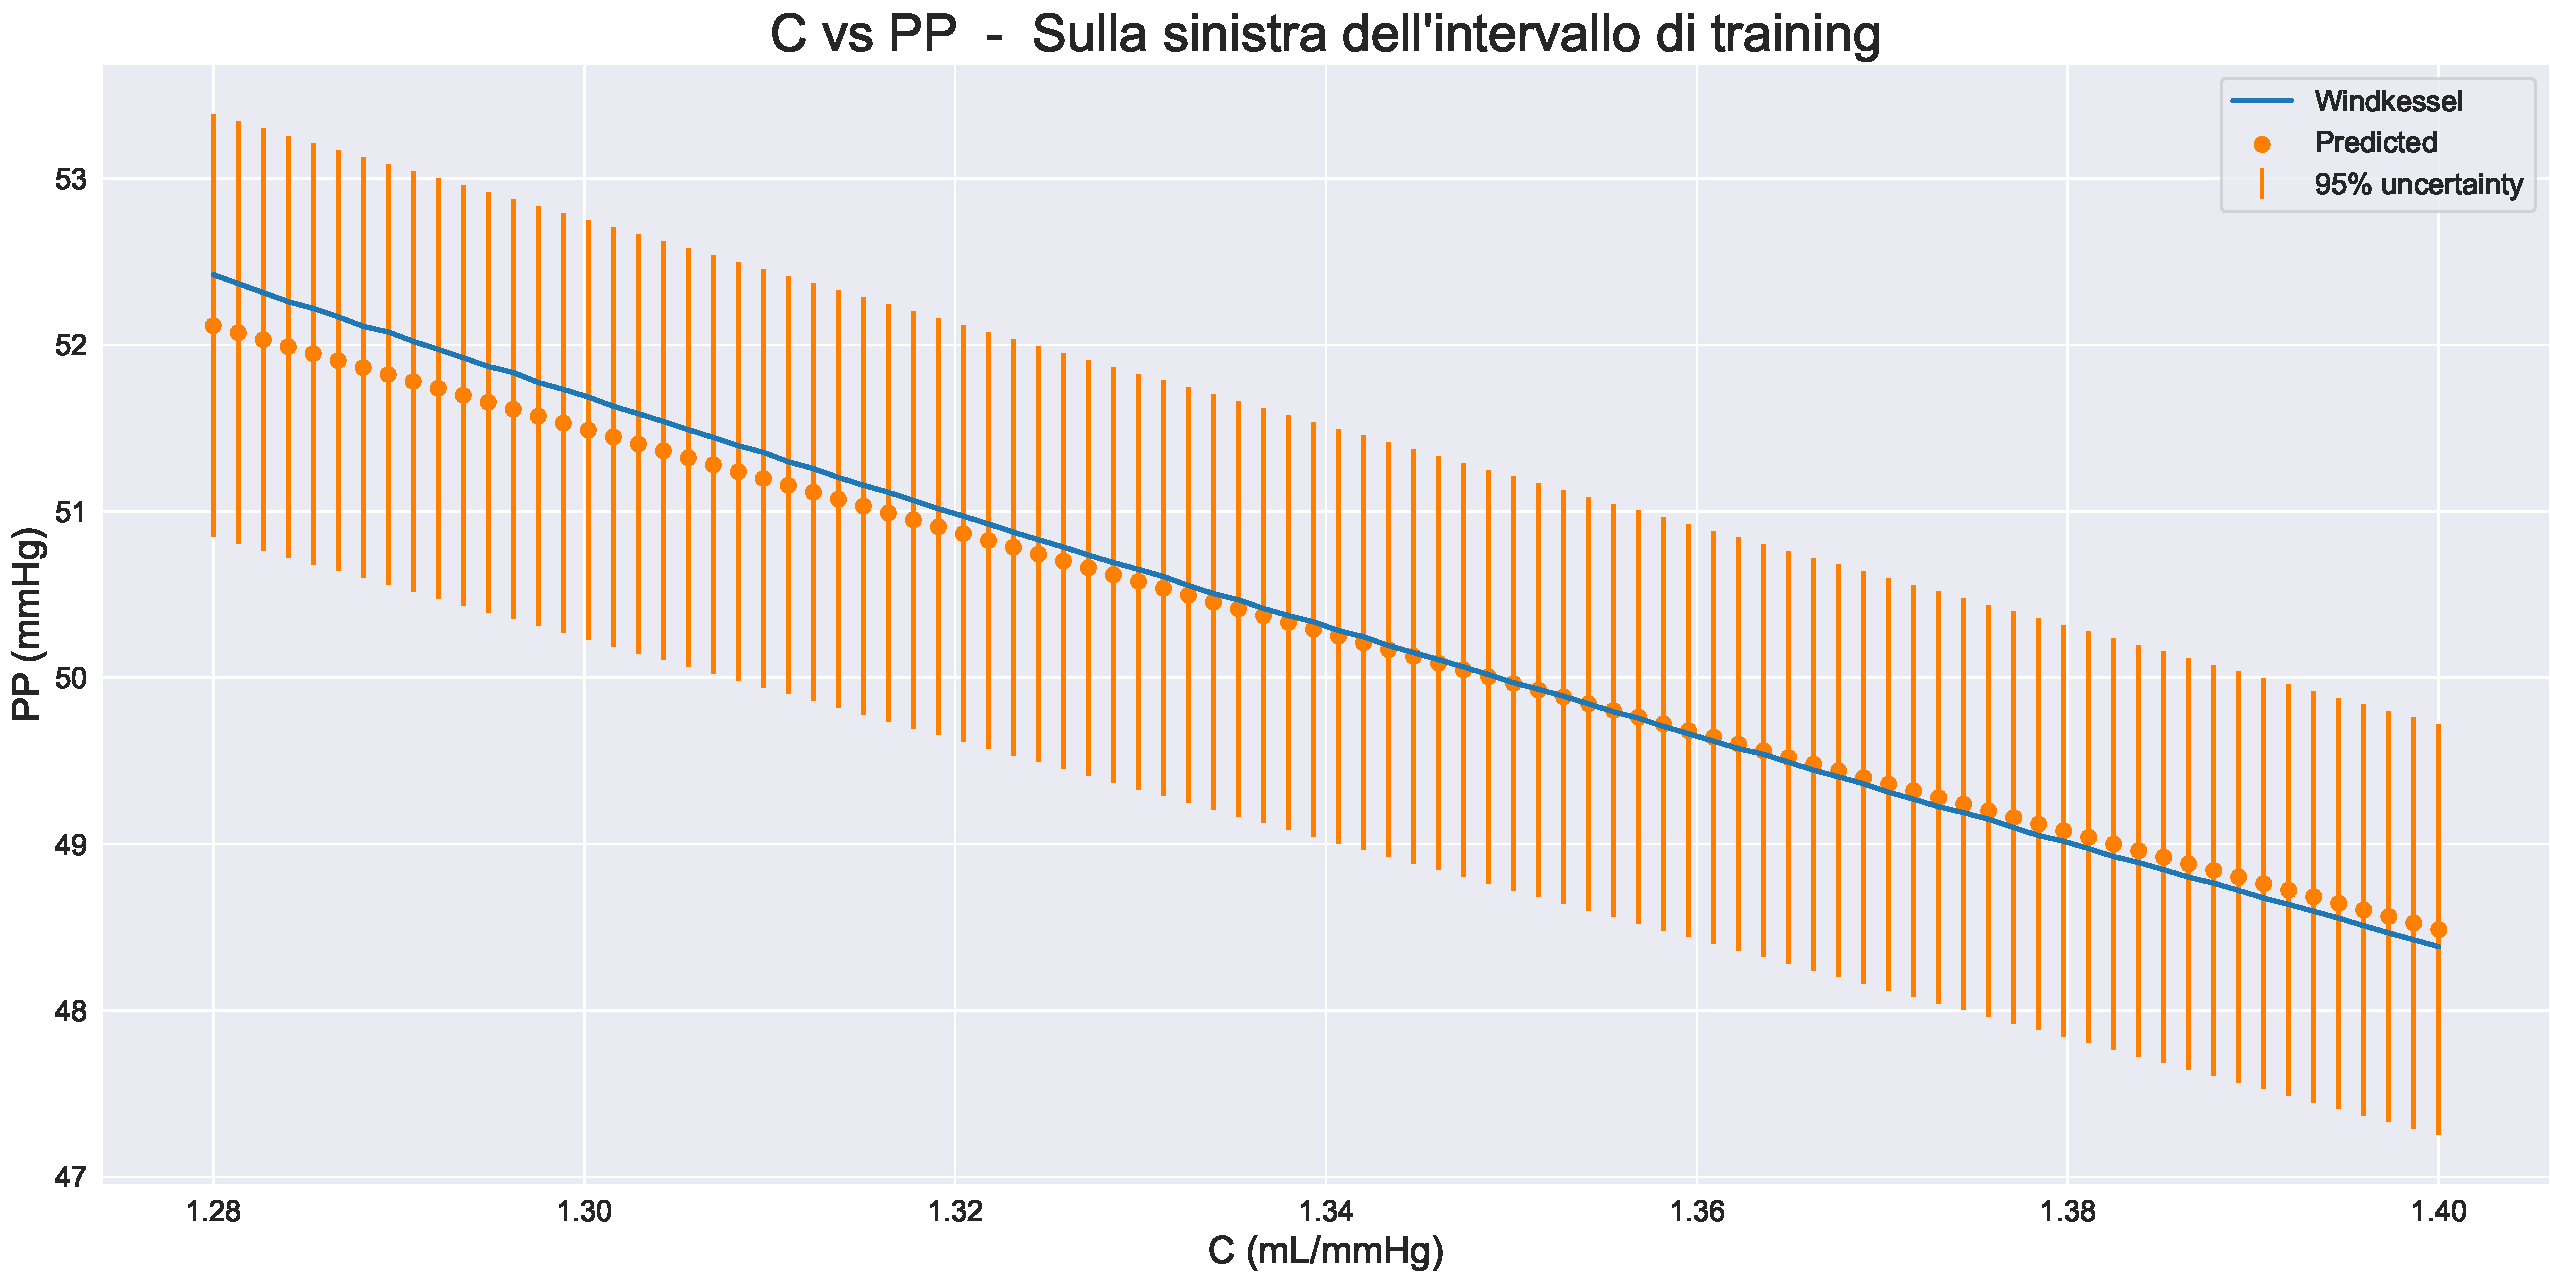
\includegraphics[width=1\textwidth]{images/Training (risultati)/PP/PP - C - sx.pdf}
    \caption{Dependence of PP on $C$ on the adjacent interval to the left of the training interval.}
    \label{PP - C - sx}
\end{figure}



\begin{figure}
    \centering
    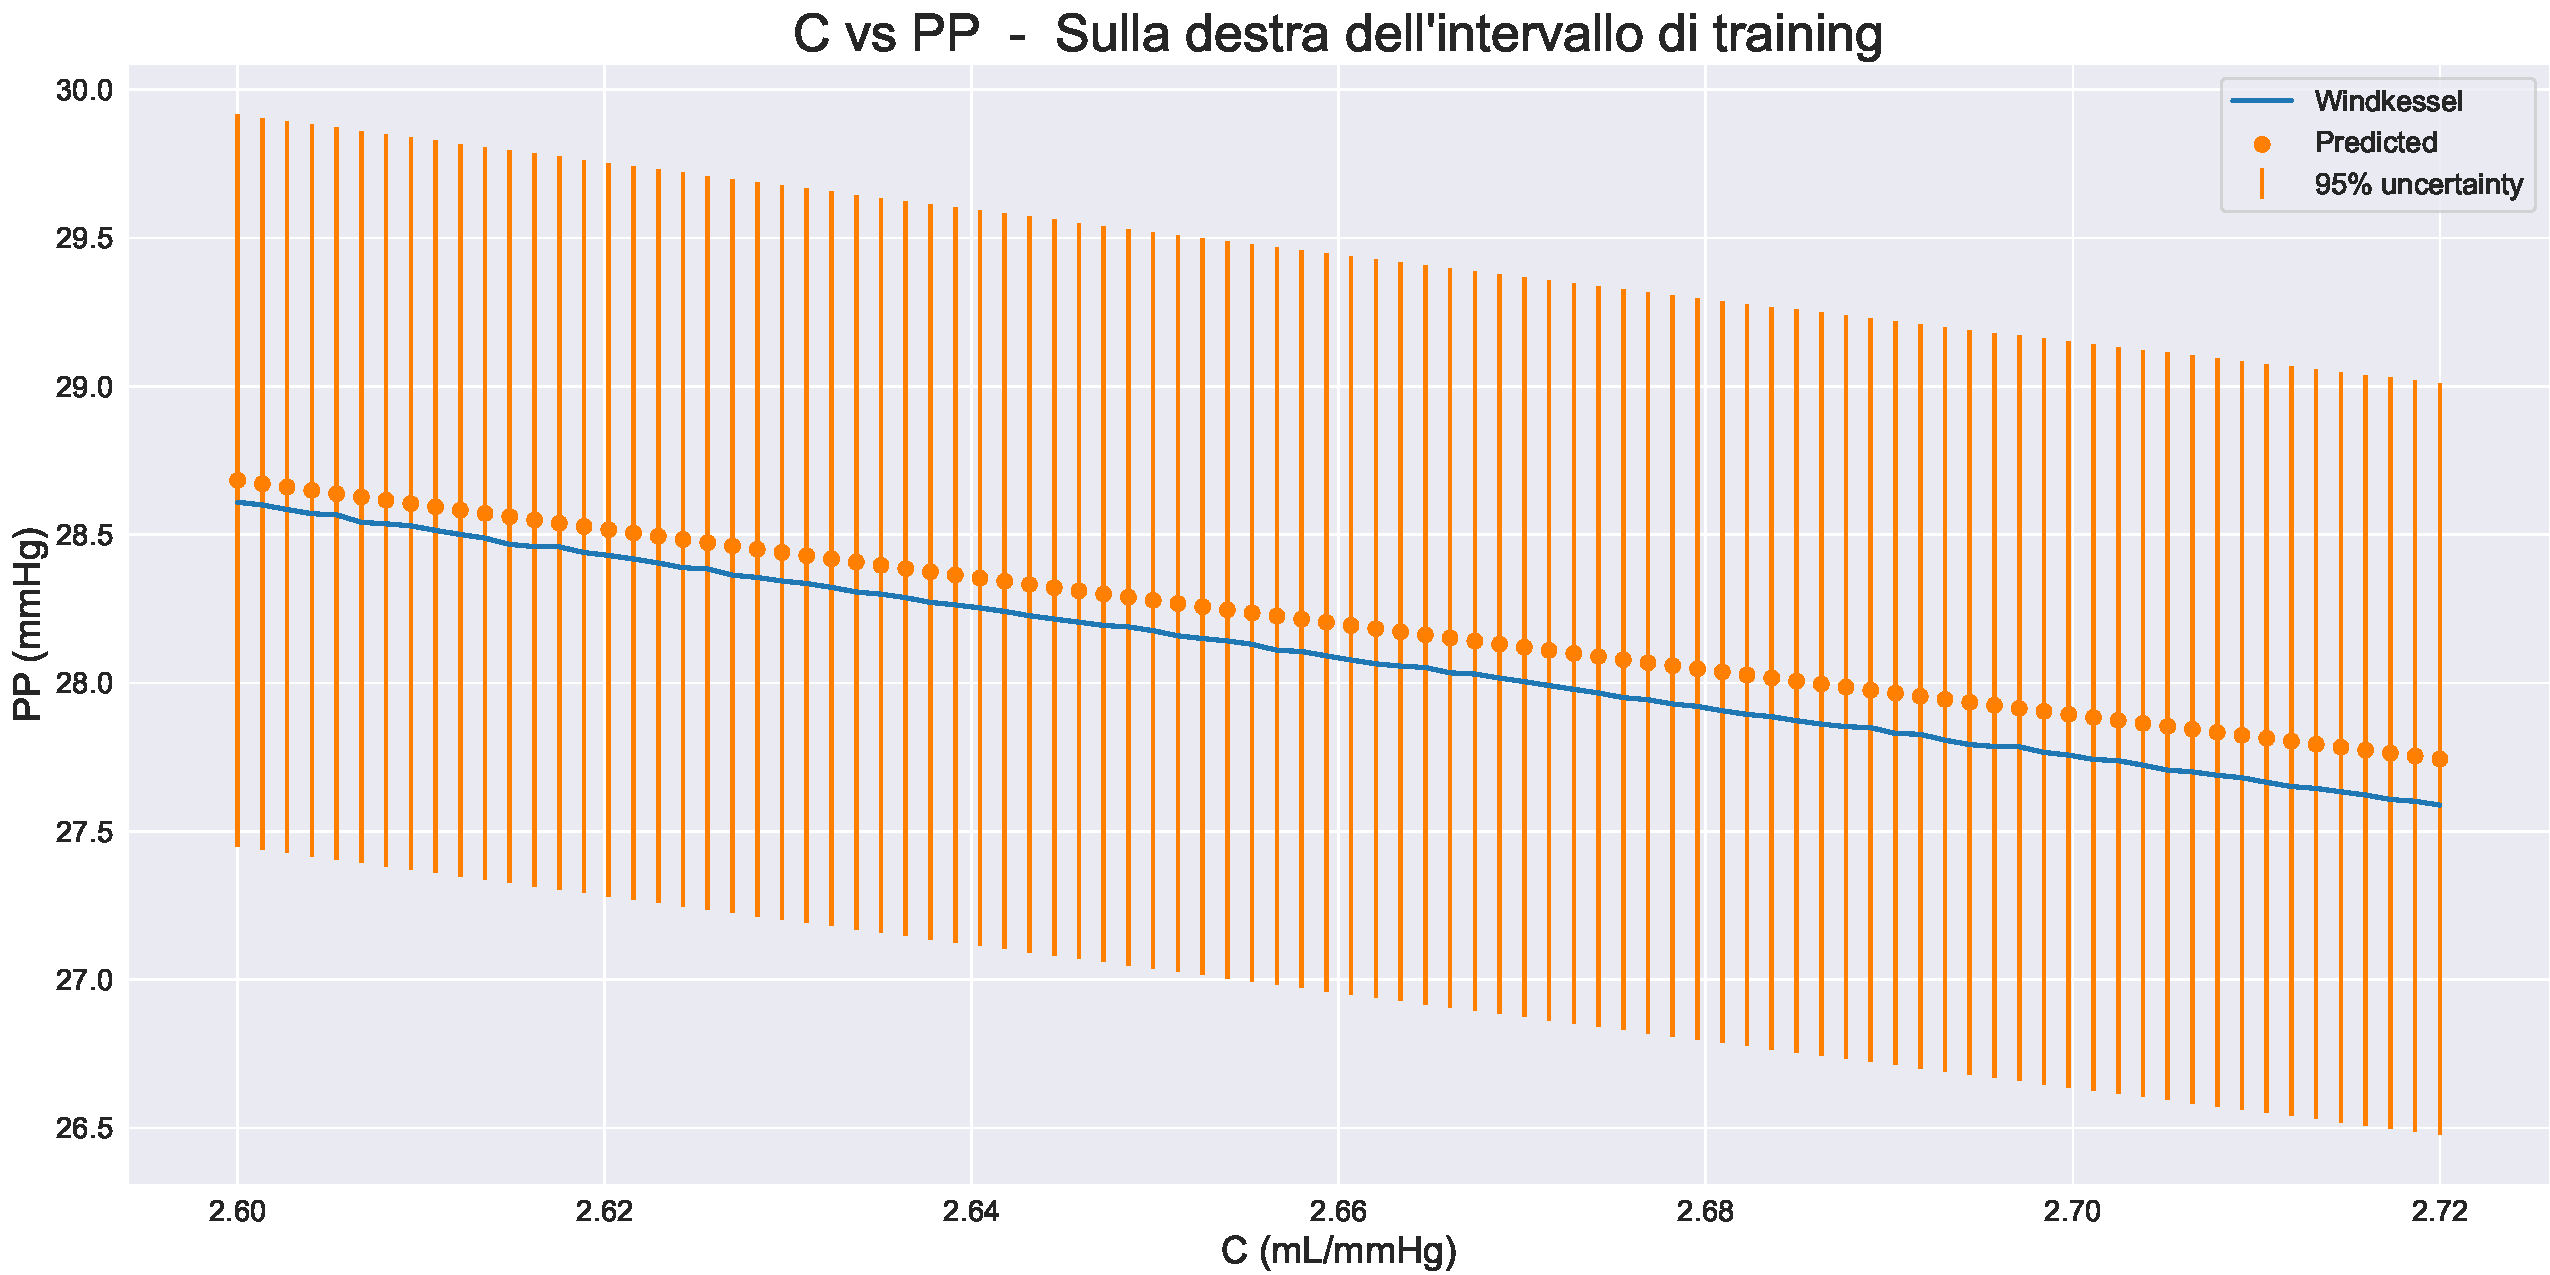
\includegraphics[width=1\textwidth]{images/Training (risultati)/PP/PP - C - dx.pdf}
    \caption{Dependence of PP on $C$ on the adjacent interval to the right of the training interval.}
    \label{PP - C - dx}
\end{figure}




\newpage
% **********
% PP - R1
% **********
\subsubsection{Dependence on $R_1$}
The overall result is shown in figure \ref{PP - R1 - full}, the result in the training interval alone in \ref{PP - R1 - training}, the result in the individual adjacent intervals in \ref{PP - R1 - sx} and \ref{PP - R1 - dx}.

\vspace{1cm}

\begin{figure}[!htb]
    \centering
    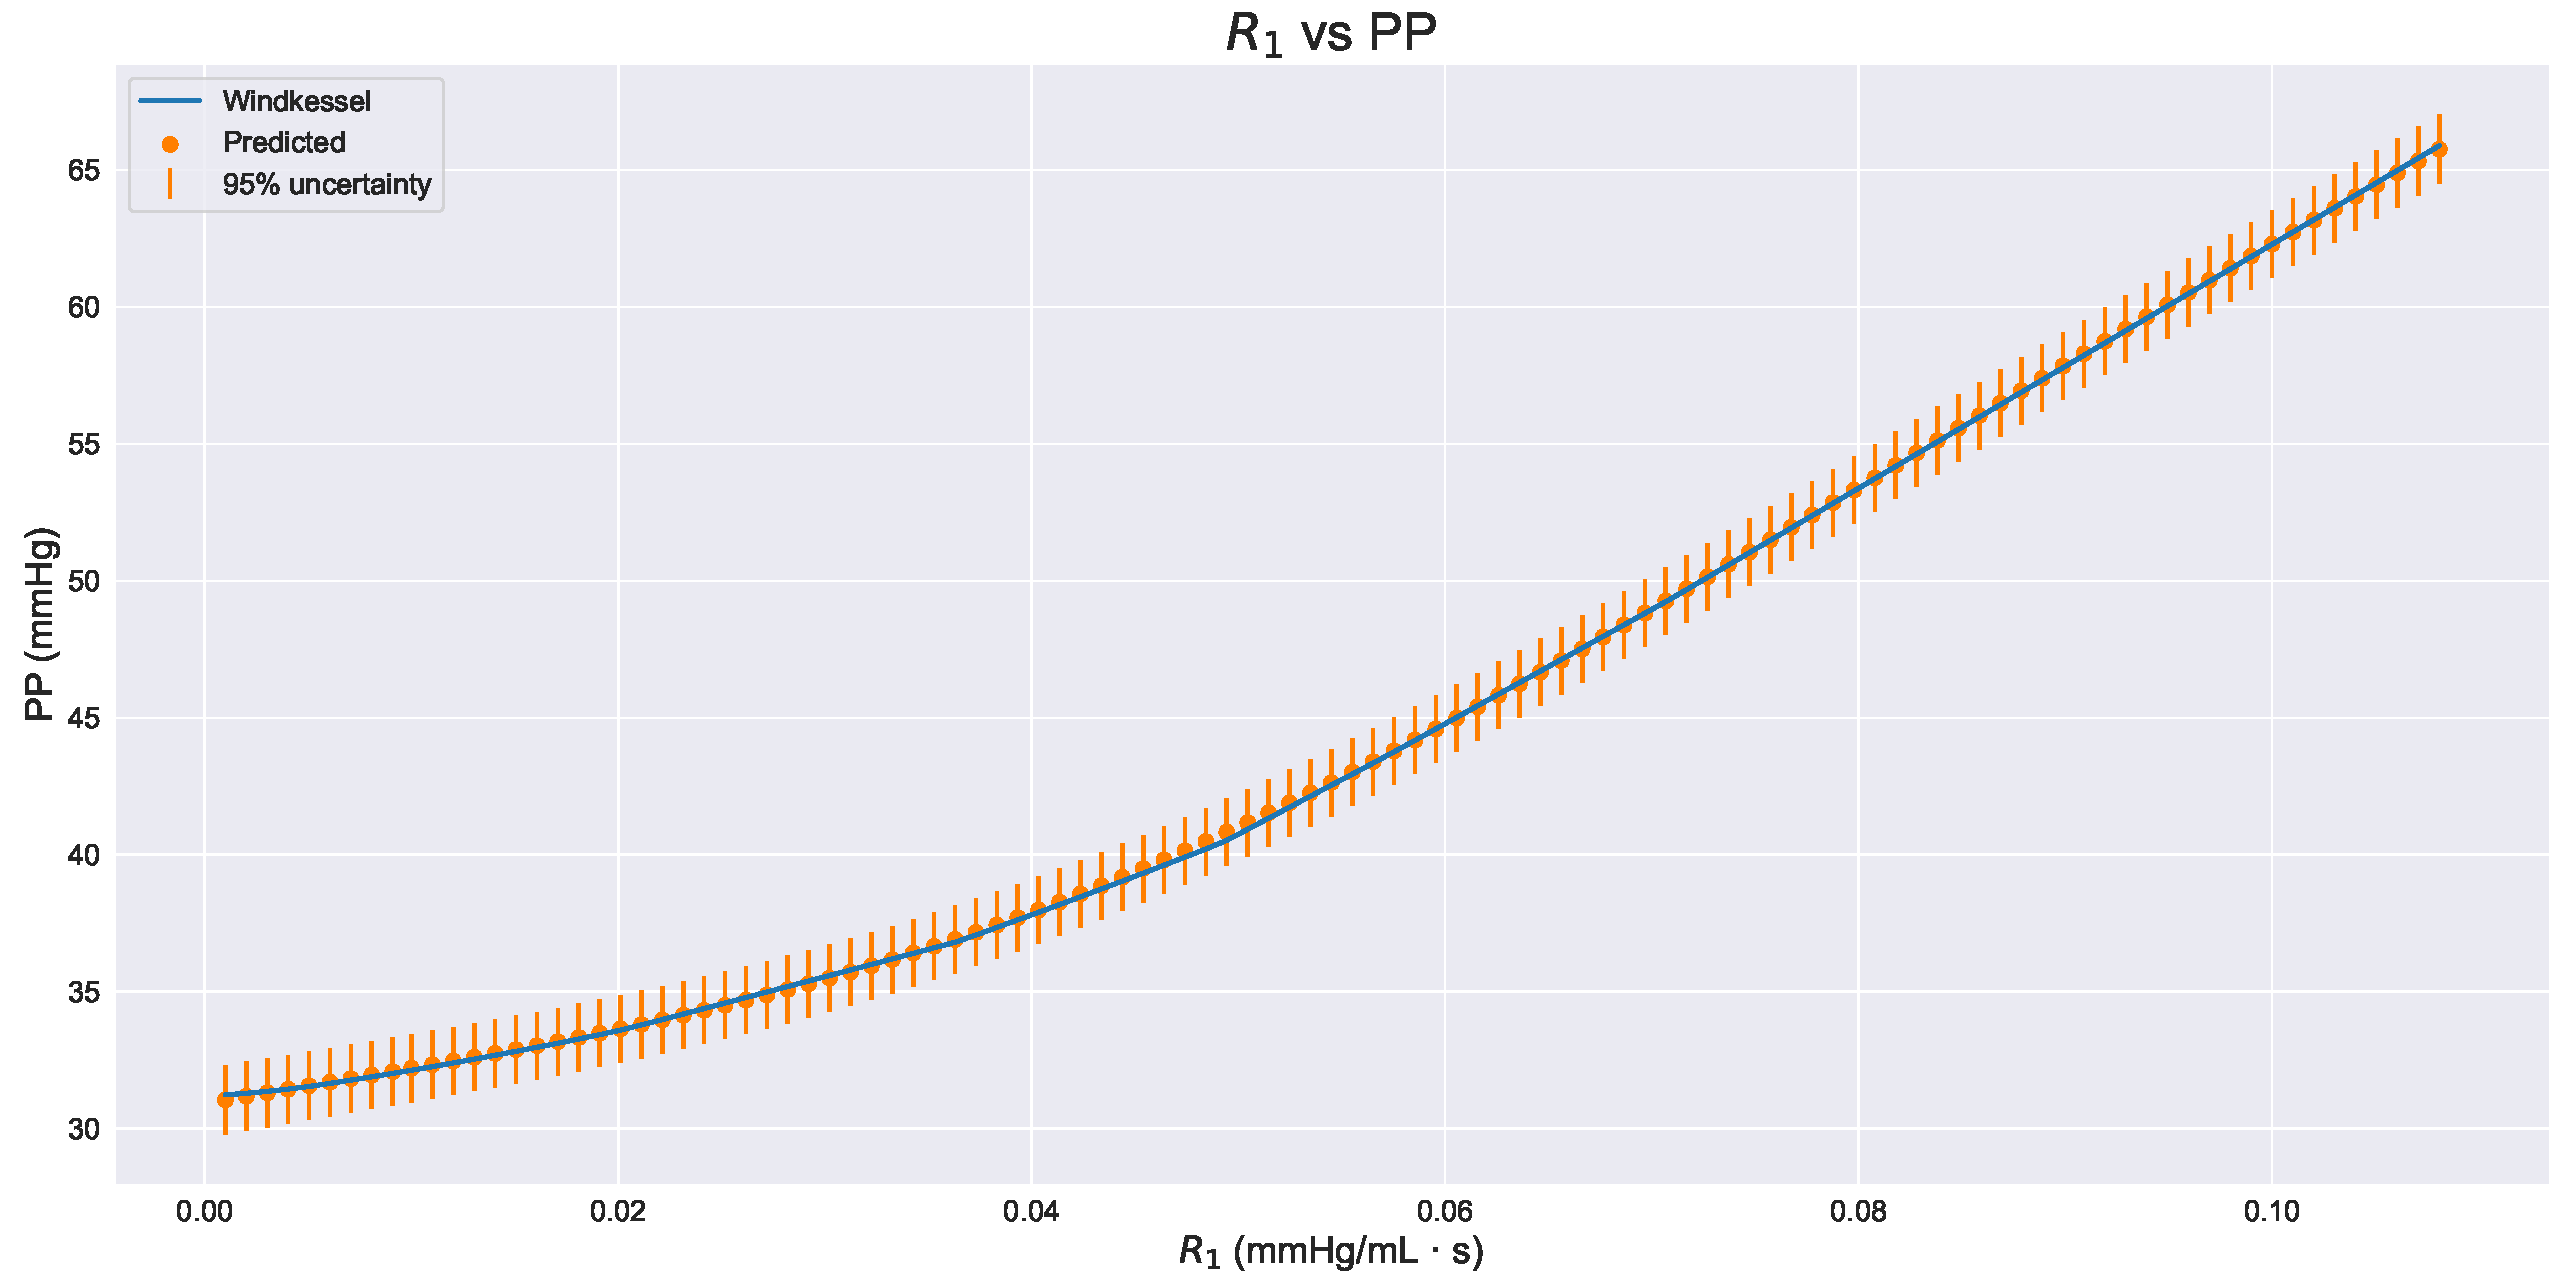
\includegraphics[width=1\textwidth]{images/Training (risultati)/PP/PP - R1 - full.pdf}
    \caption{Dependence of PP on $R1$ on the training interval and two adjacent intervals.}
    \label{PP - R1 - full}
\end{figure}

\vspace{0.32cm}

\begin{figure}[!htb]
    \centering
    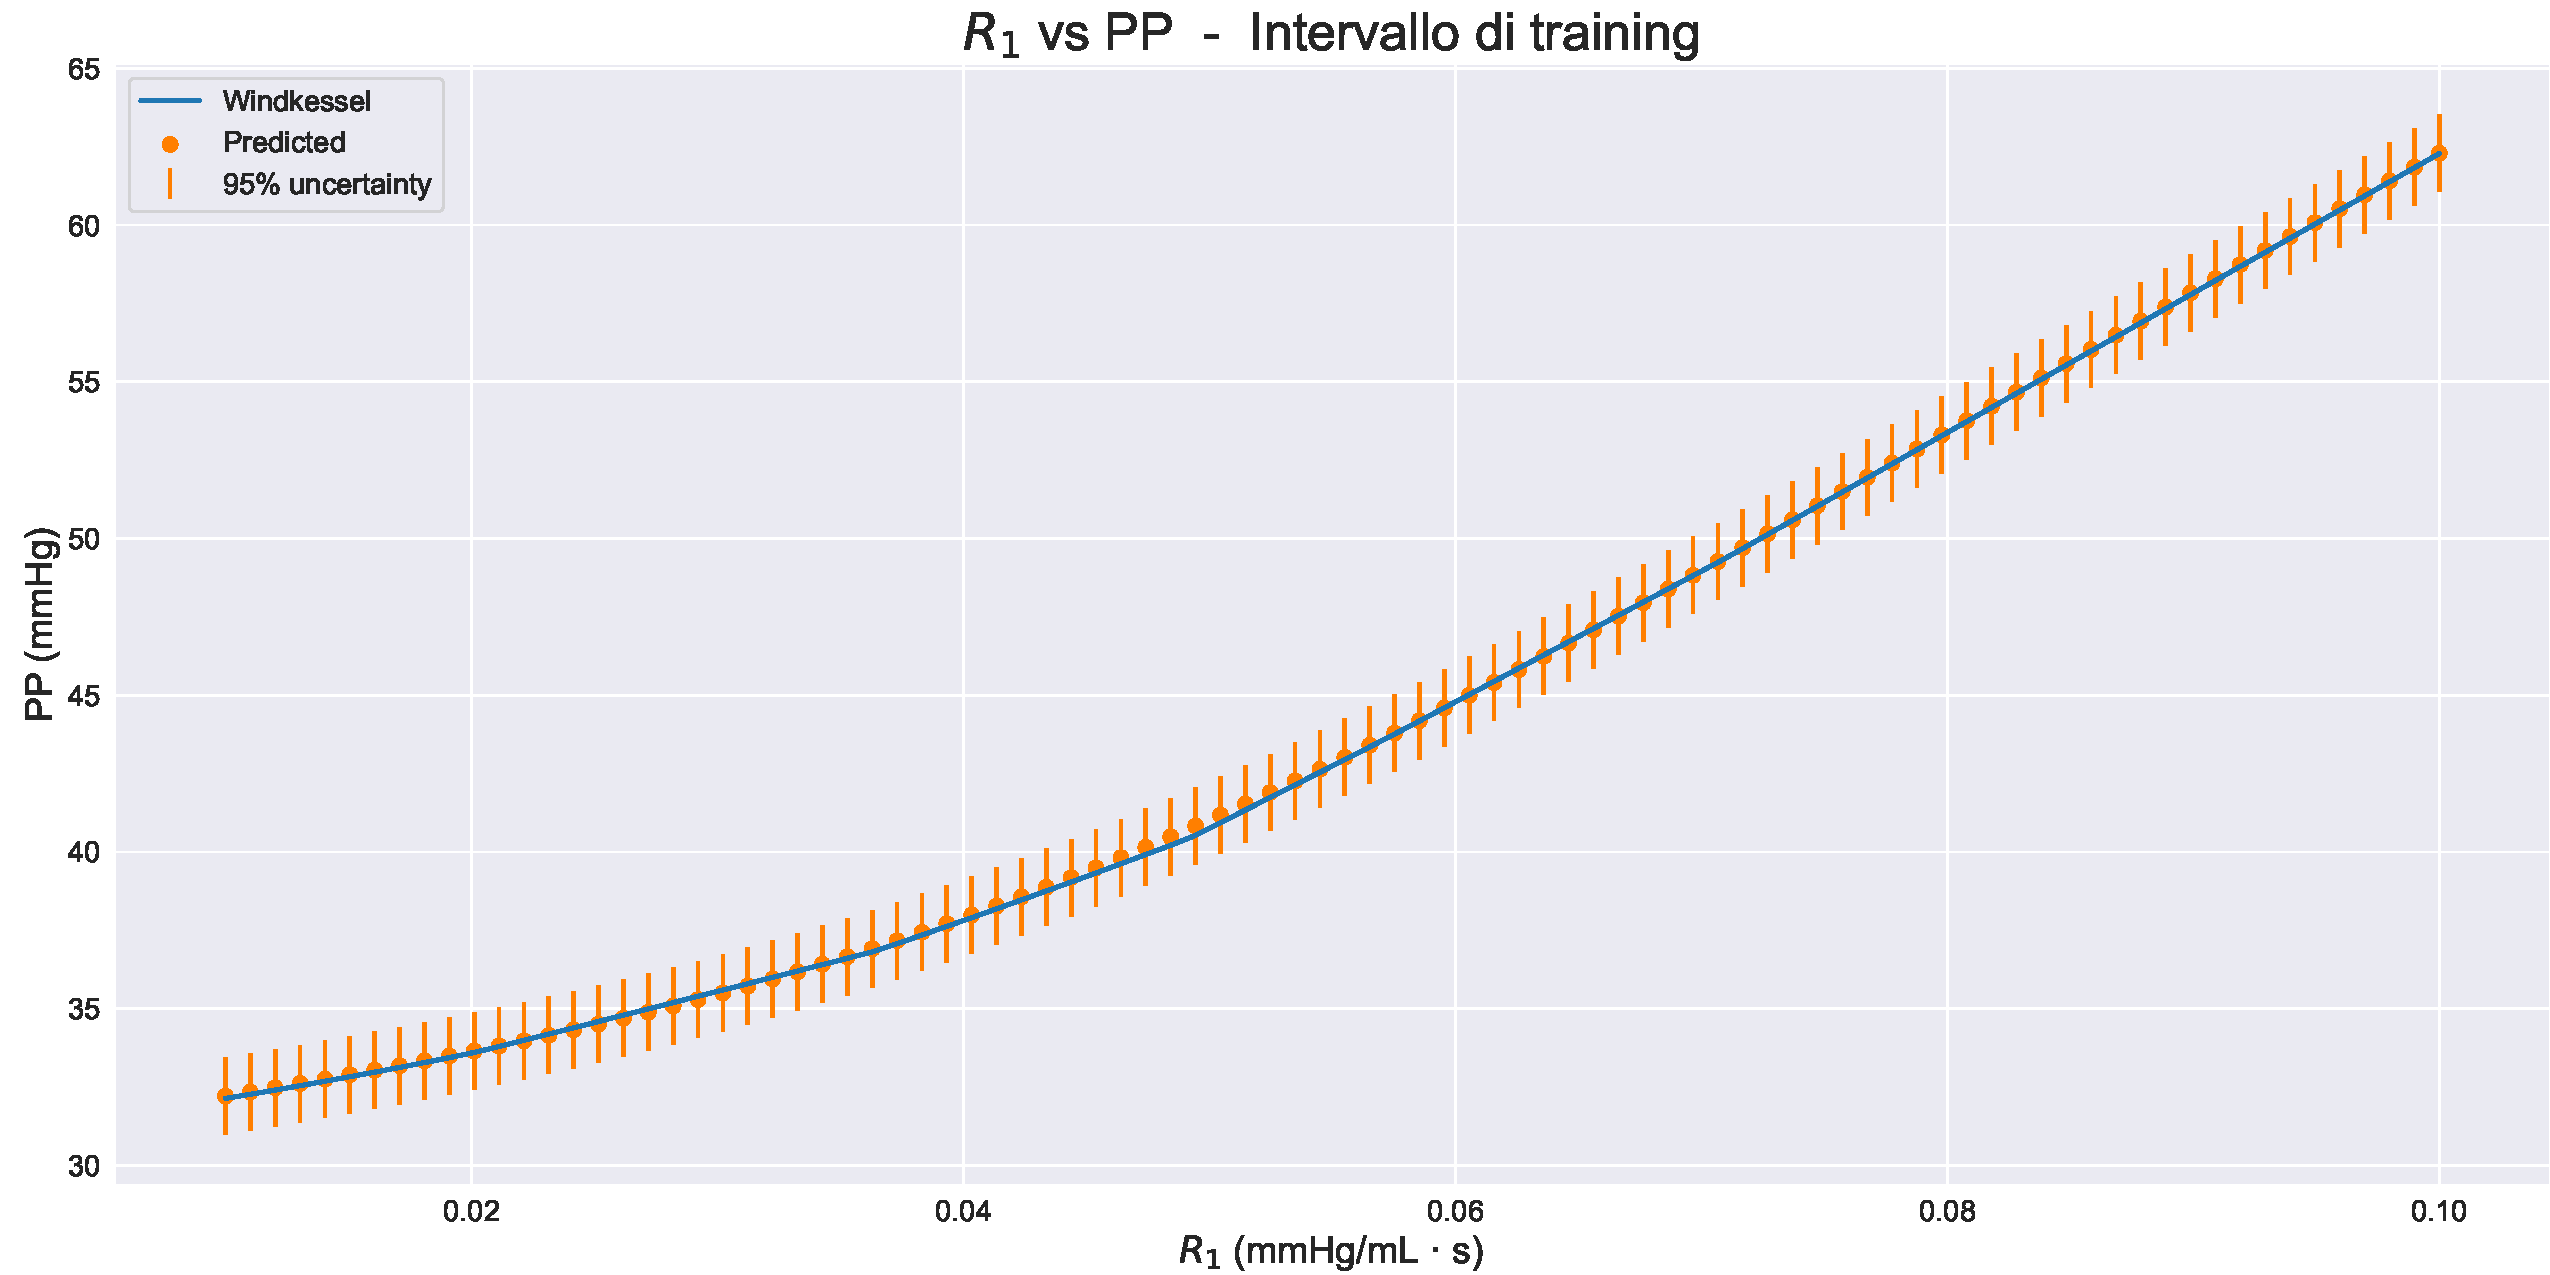
\includegraphics[width=1\textwidth]{images/Training (risultati)/PP/PP - R1 - training.pdf}
    \caption{Dependence of PP on $R1$ over the training interval.}
    \label{PP - R1 - training}
\end{figure}

\begin{figure}
    \centering
    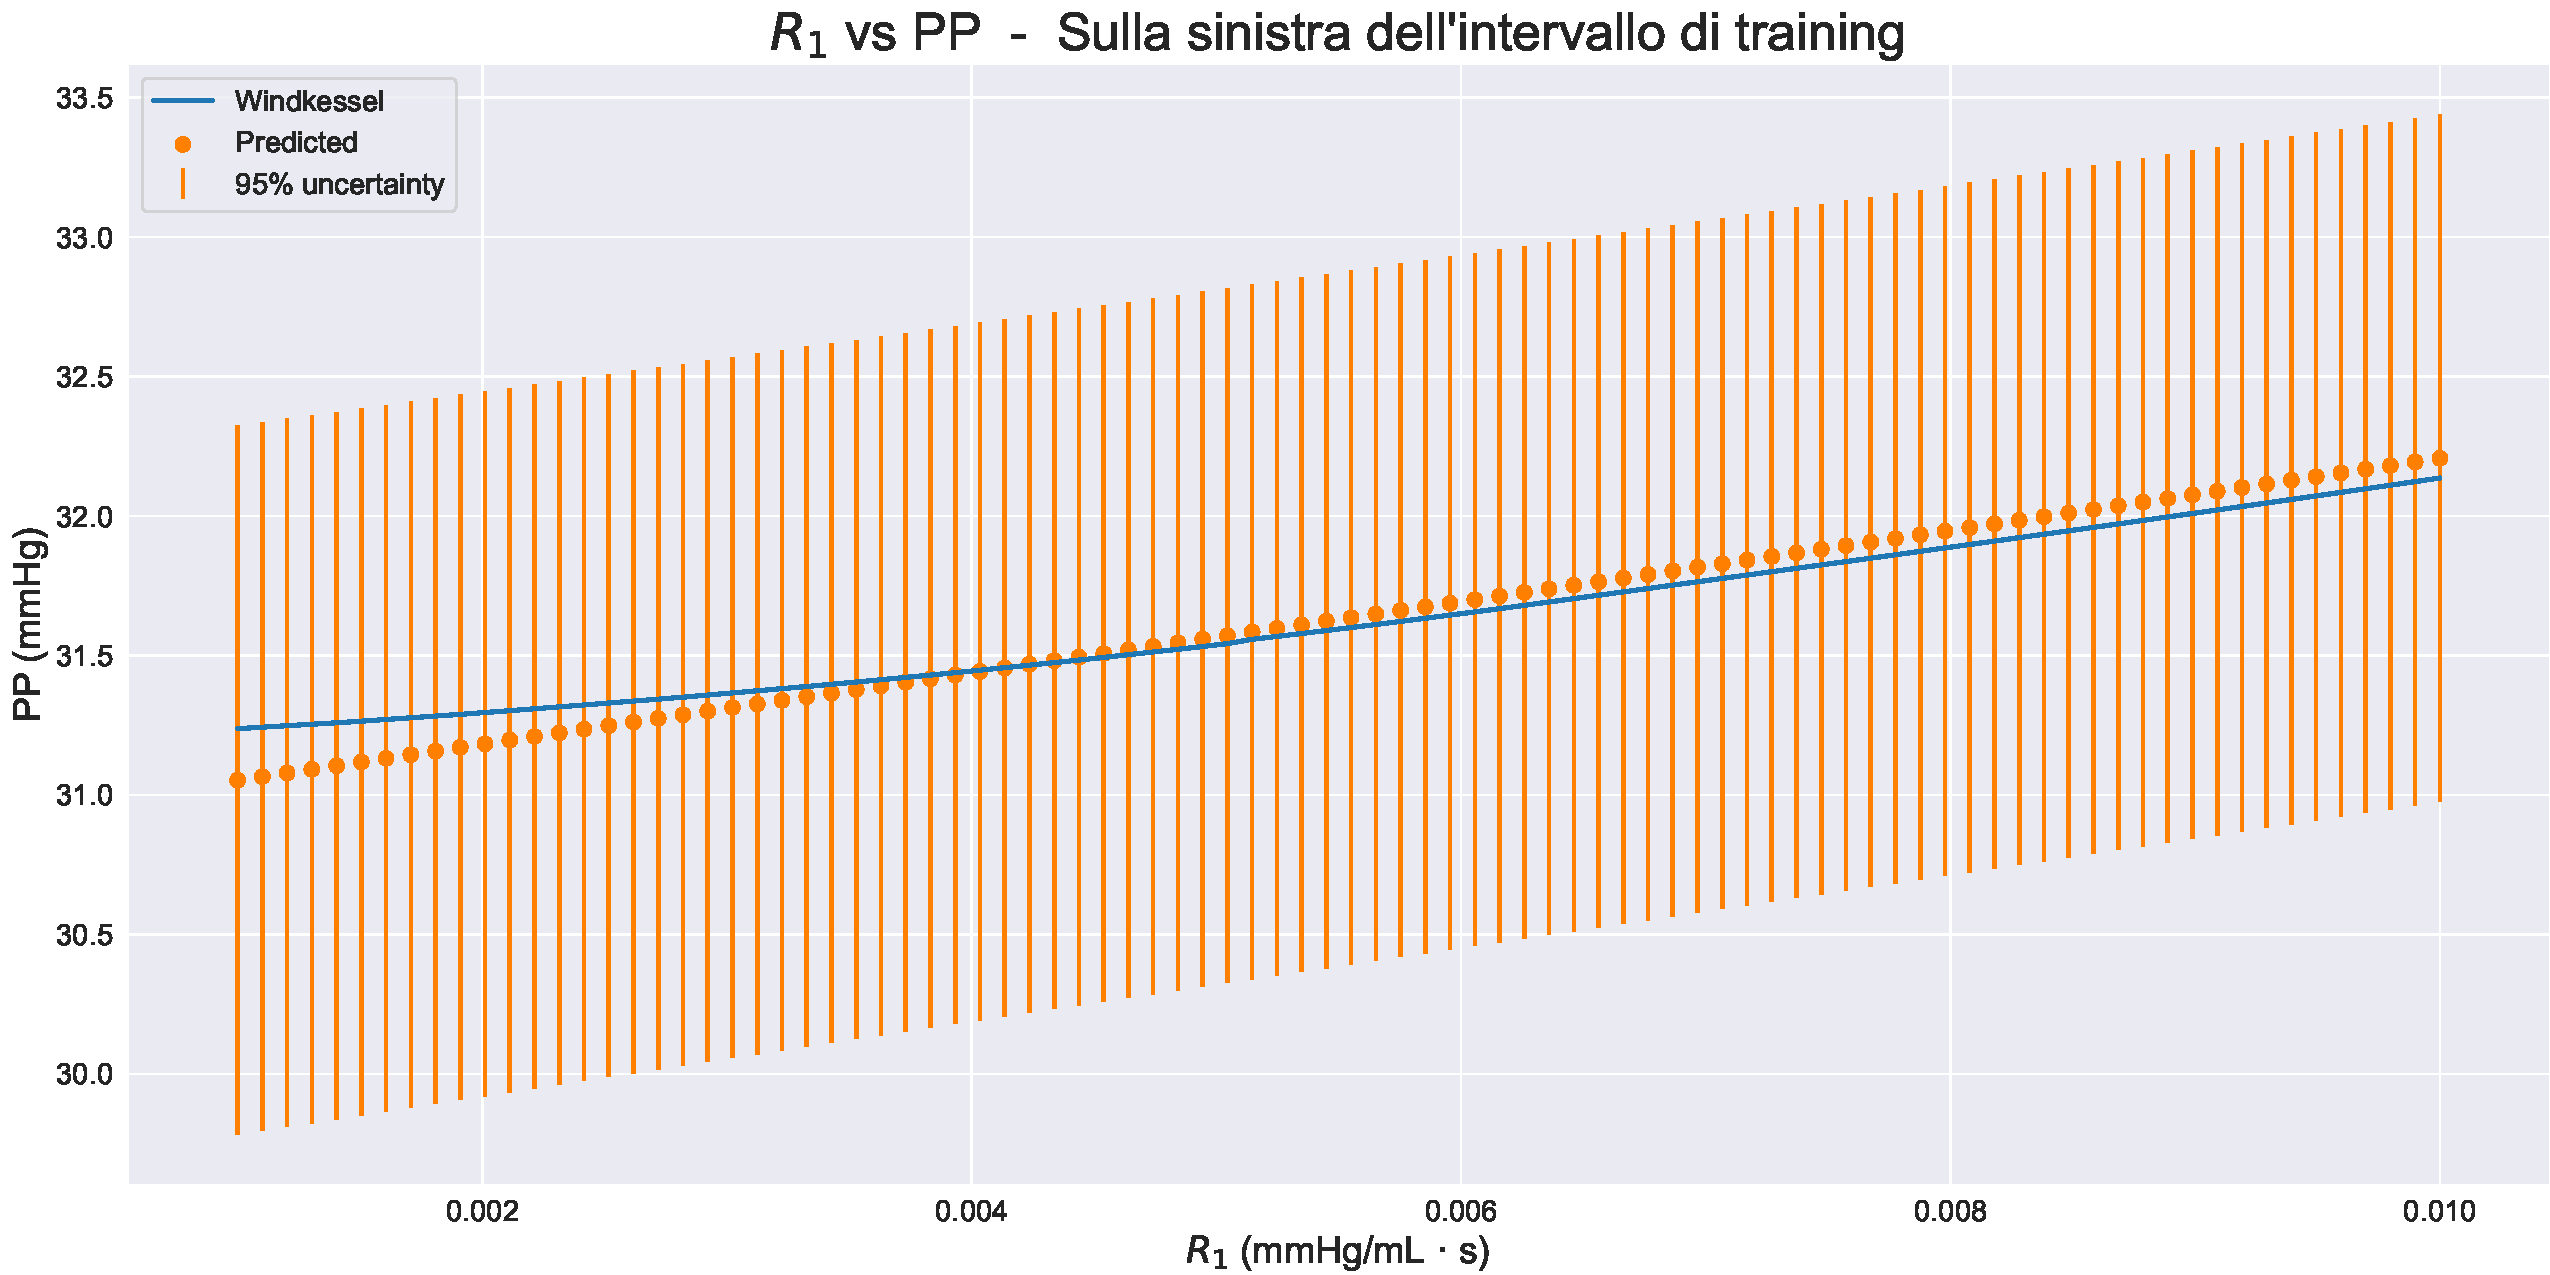
\includegraphics[width=1\textwidth]{images/Training (risultati)/PP/PP - R1 - sx.pdf}
    \caption{Dependence of PP on $R1$ on the adjoint interval to the left of the training interval.}
    \label{PP - R1 - sx}
\end{figure}



\begin{figure}
    \centering
    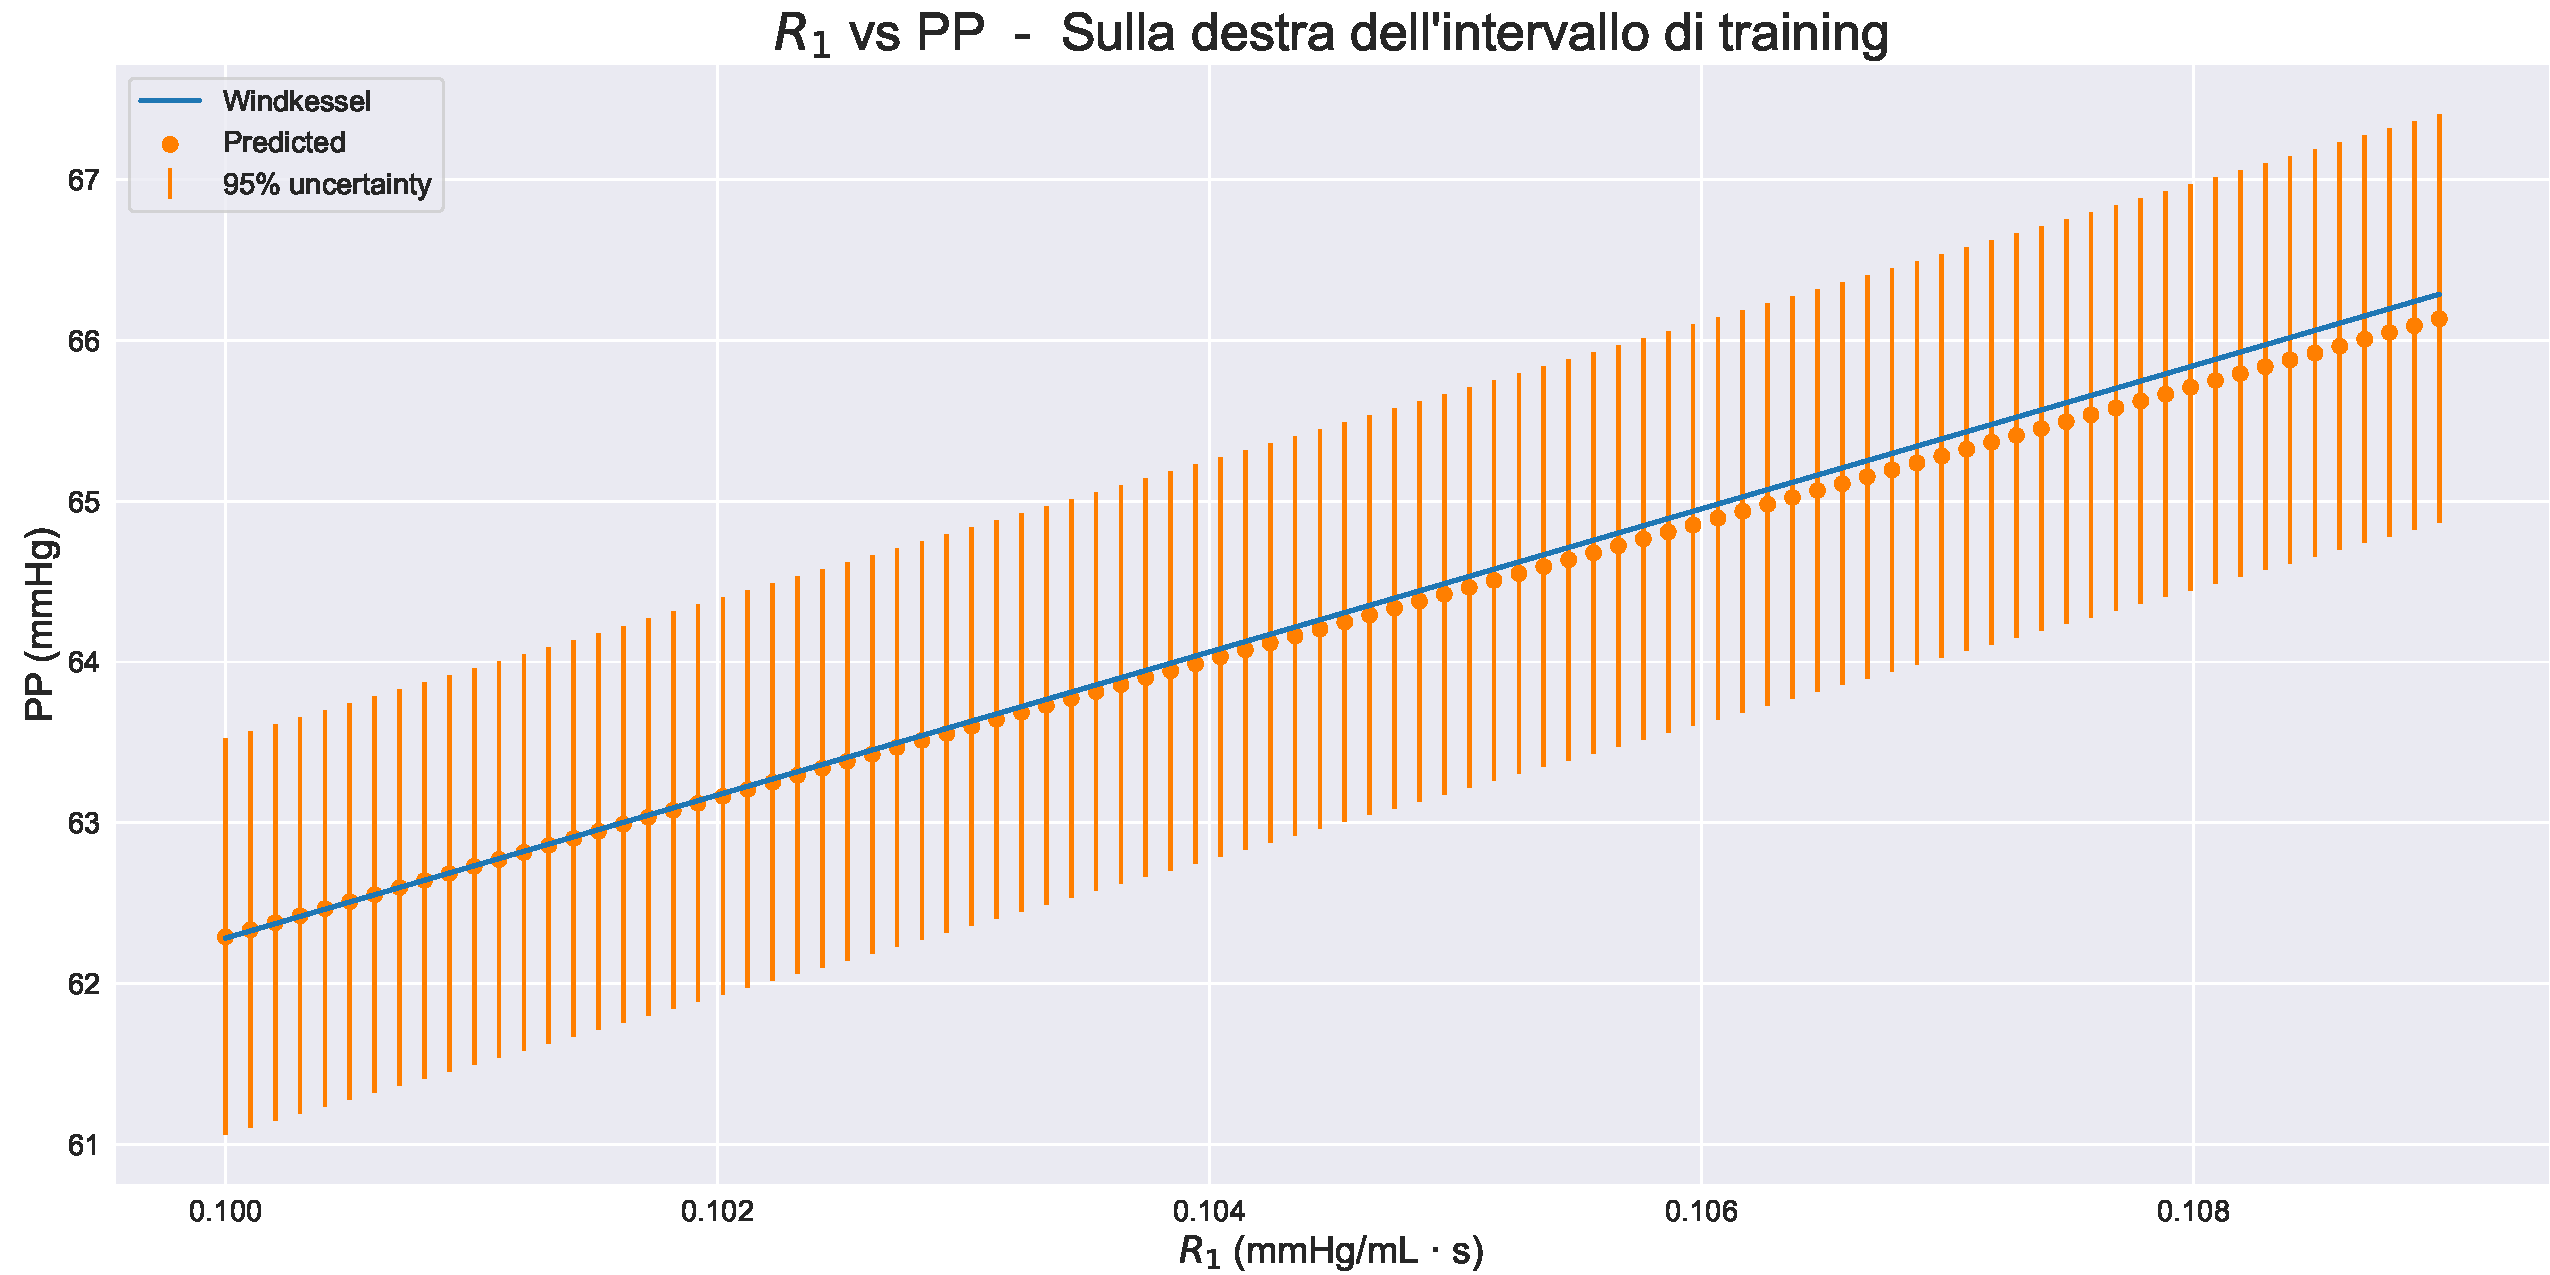
\includegraphics[width=1\textwidth]{images/Training (risultati)/PP/PP - R1 - dx.pdf}
    \caption{Dependence of PP on $R1$ on the adjacent interval to the right of the training interval.}
    \label{PP - R1 - dx}
\end{figure}

\newpage


% **********
% PP - R2
% **********
\subsubsection{Dependence on $R_2$}
The overall result is shown in figure \ref{PP - R2 - full}, the result in the training interval alone in \ref{PP - R2 - training}, the result in the individual adjacent intervals in \ref{PP - R2 - sx} and \ref{PP - R2 - dx}.

\vspace{0.9cm}

\begin{figure}[!htb]
    \centering
    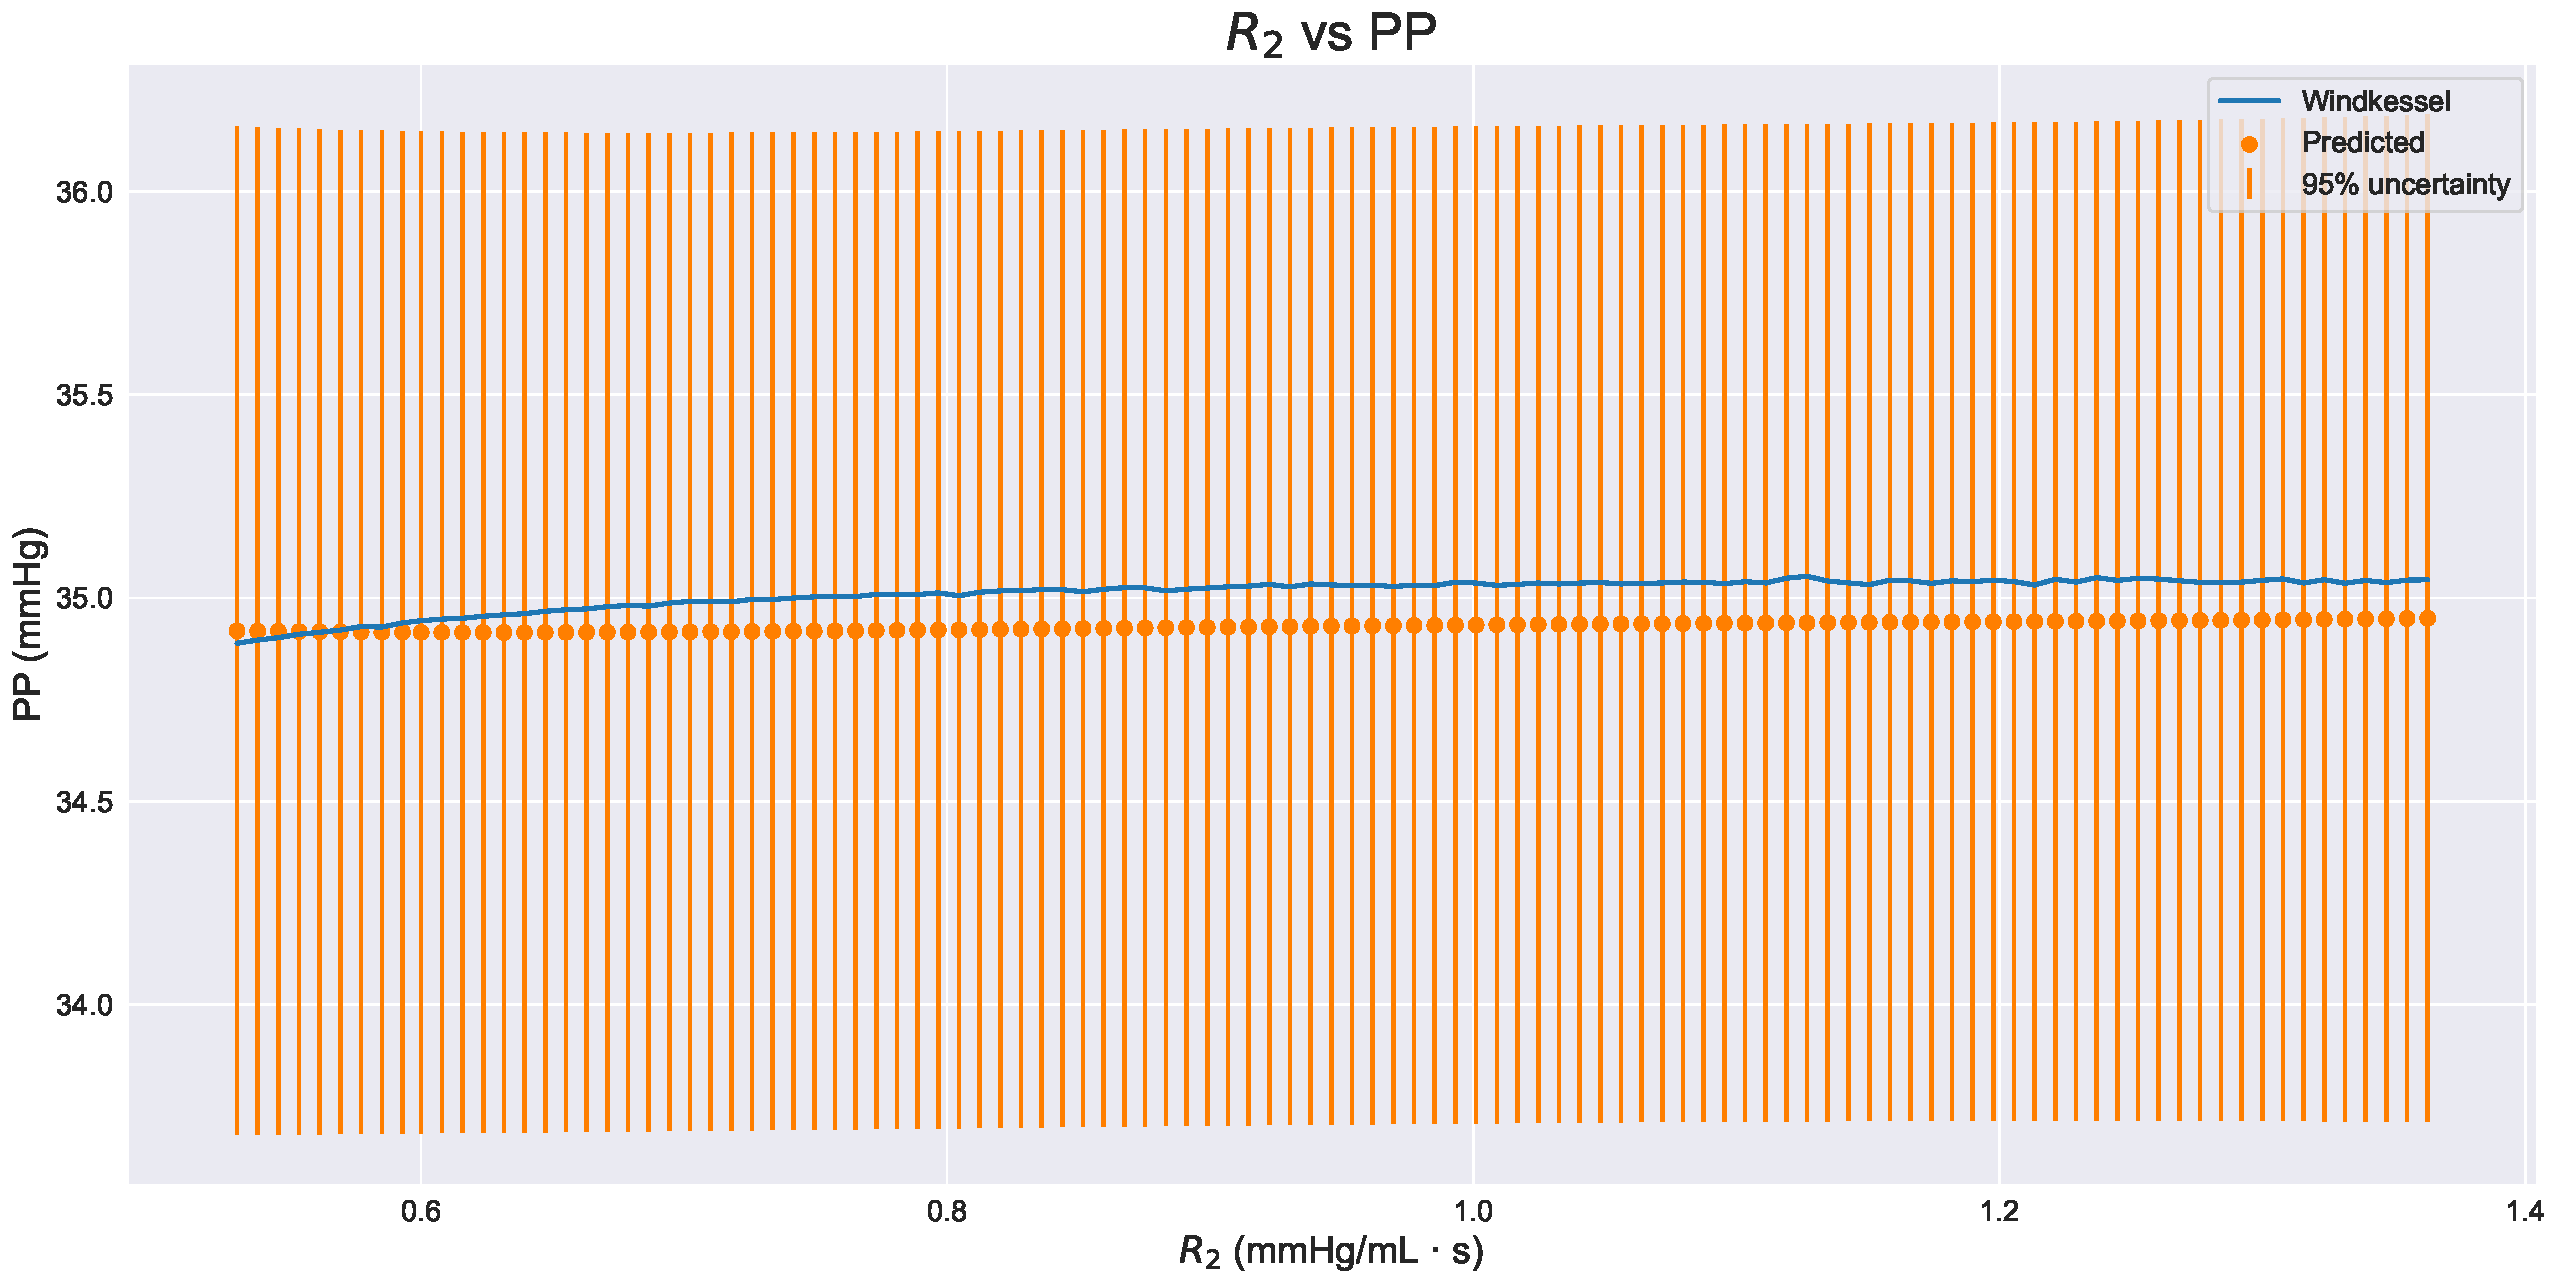
\includegraphics[width=1\textwidth]{images/Training (risultati)/PP/PP - R2 - full.pdf}
    \caption{Dependence of PP on $R2$ on the training interval and two adjacent intervals.}
    \label{PP - R2 - full}
\end{figure}

\vspace{0.32cm}

\begin{figure}[!htb]
    \centering
    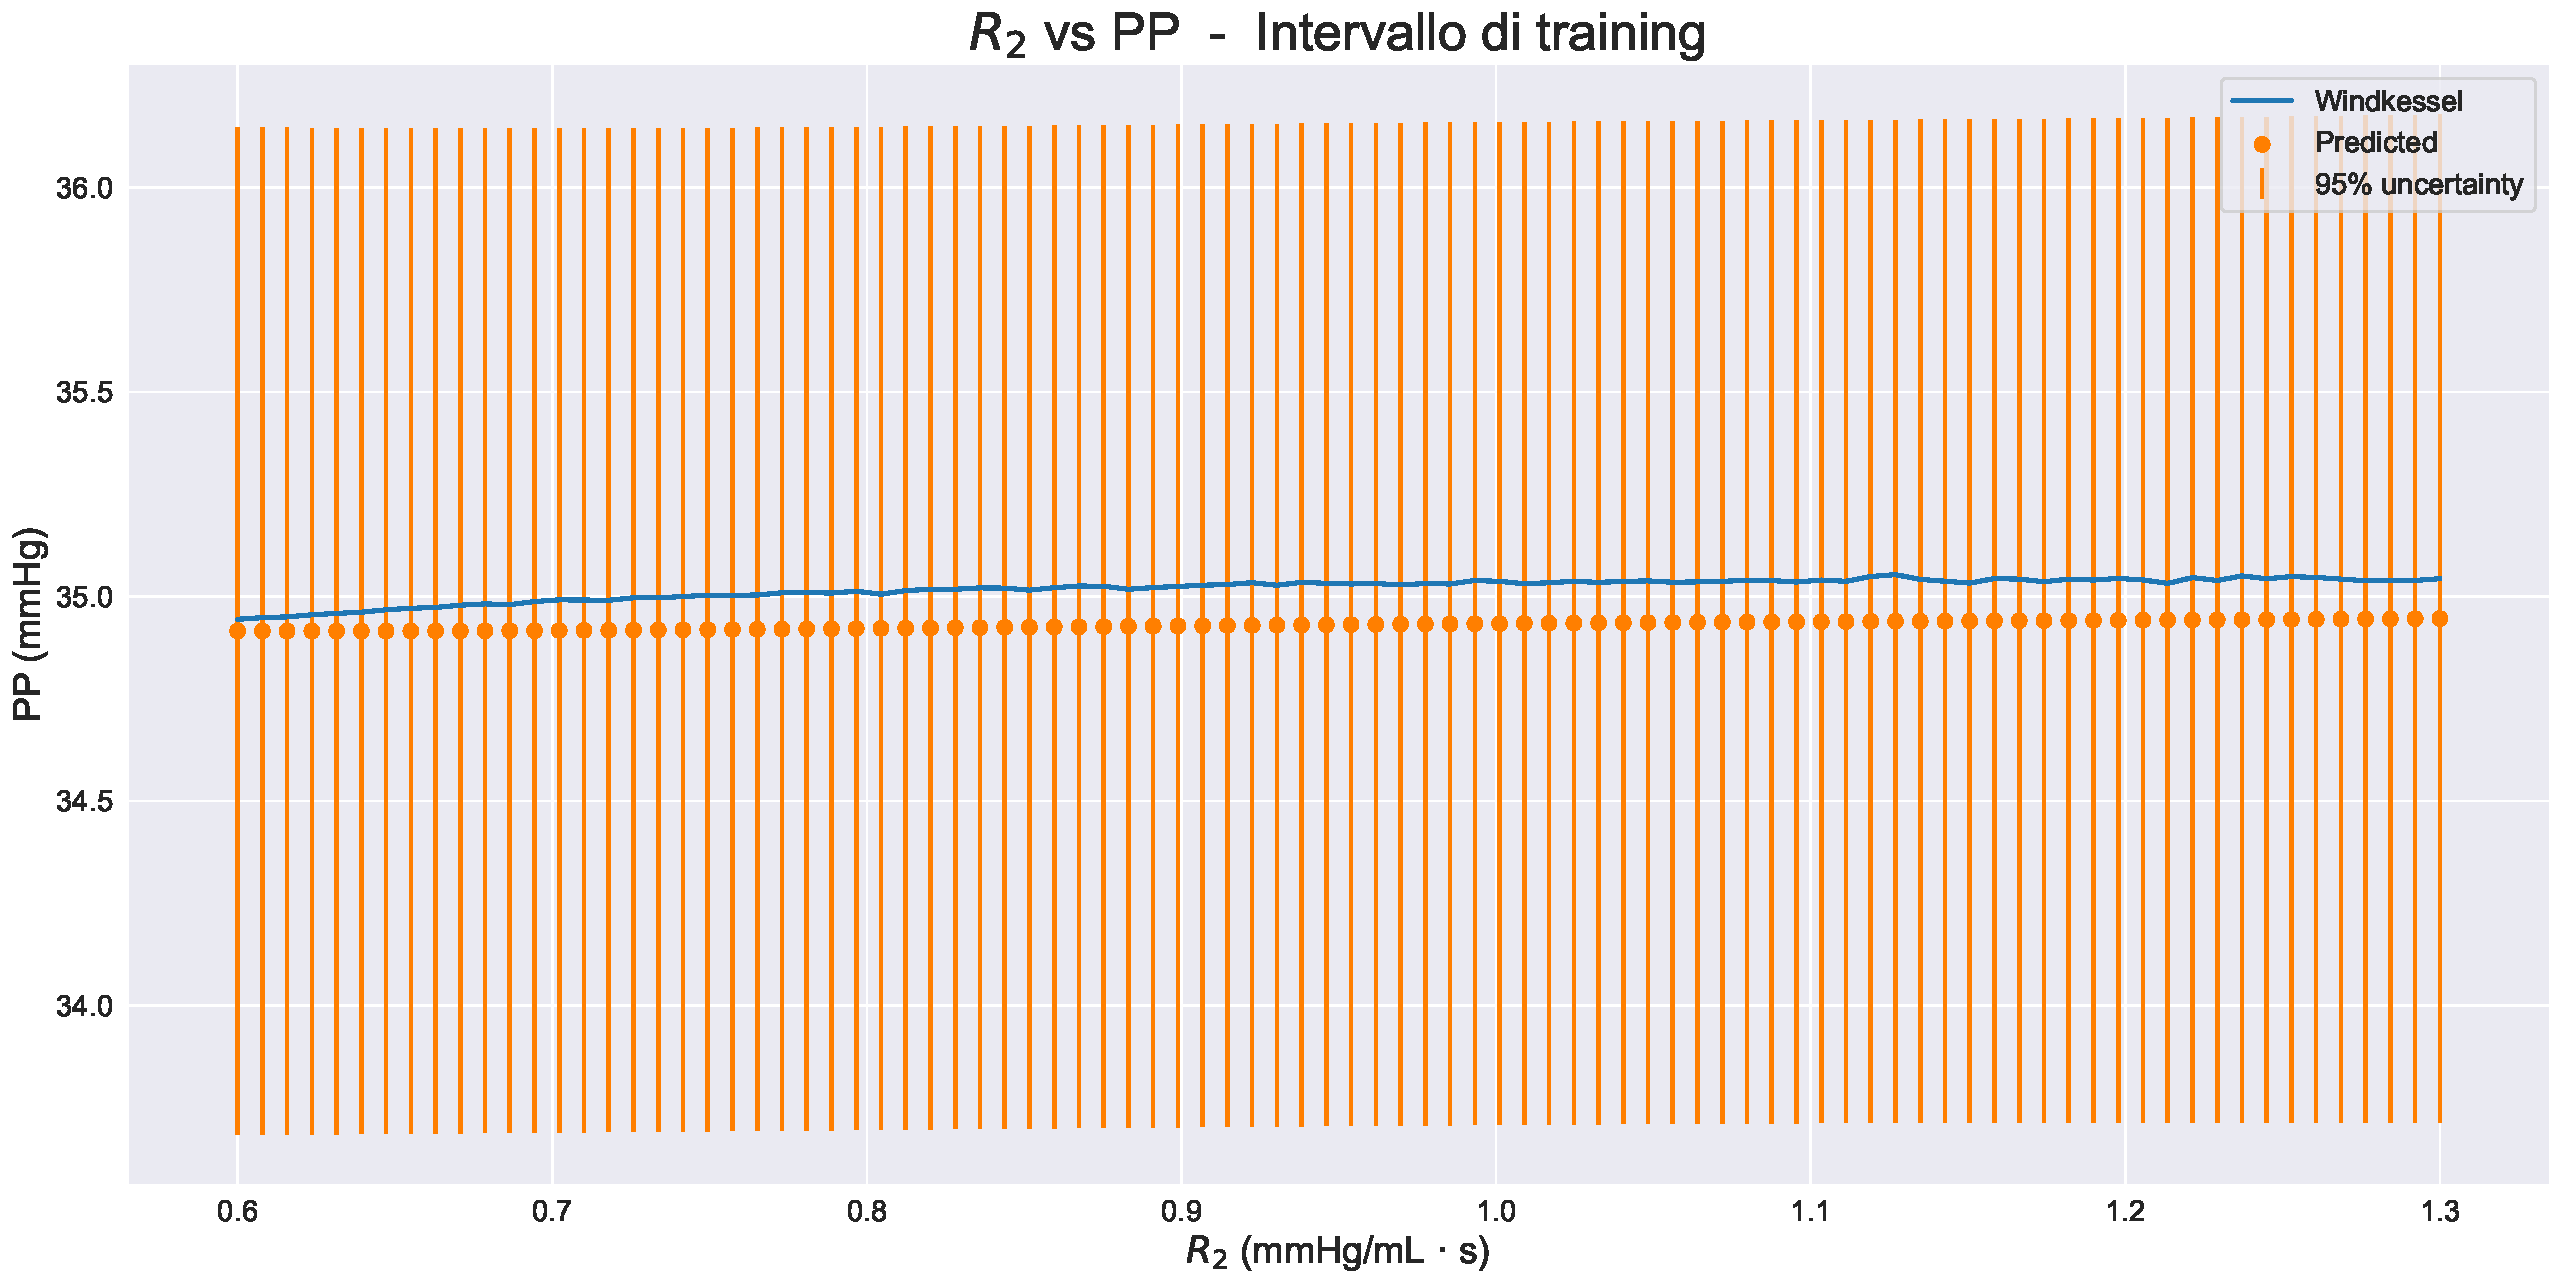
\includegraphics[width=1\textwidth]{images/Training (risultati)/PP/PP - R2 - training.pdf}
    \caption{Dependence of PP on $R2$ over the training interval.}
    \label{PP - R2 - training}
\end{figure}

\begin{figure}
    \centering
    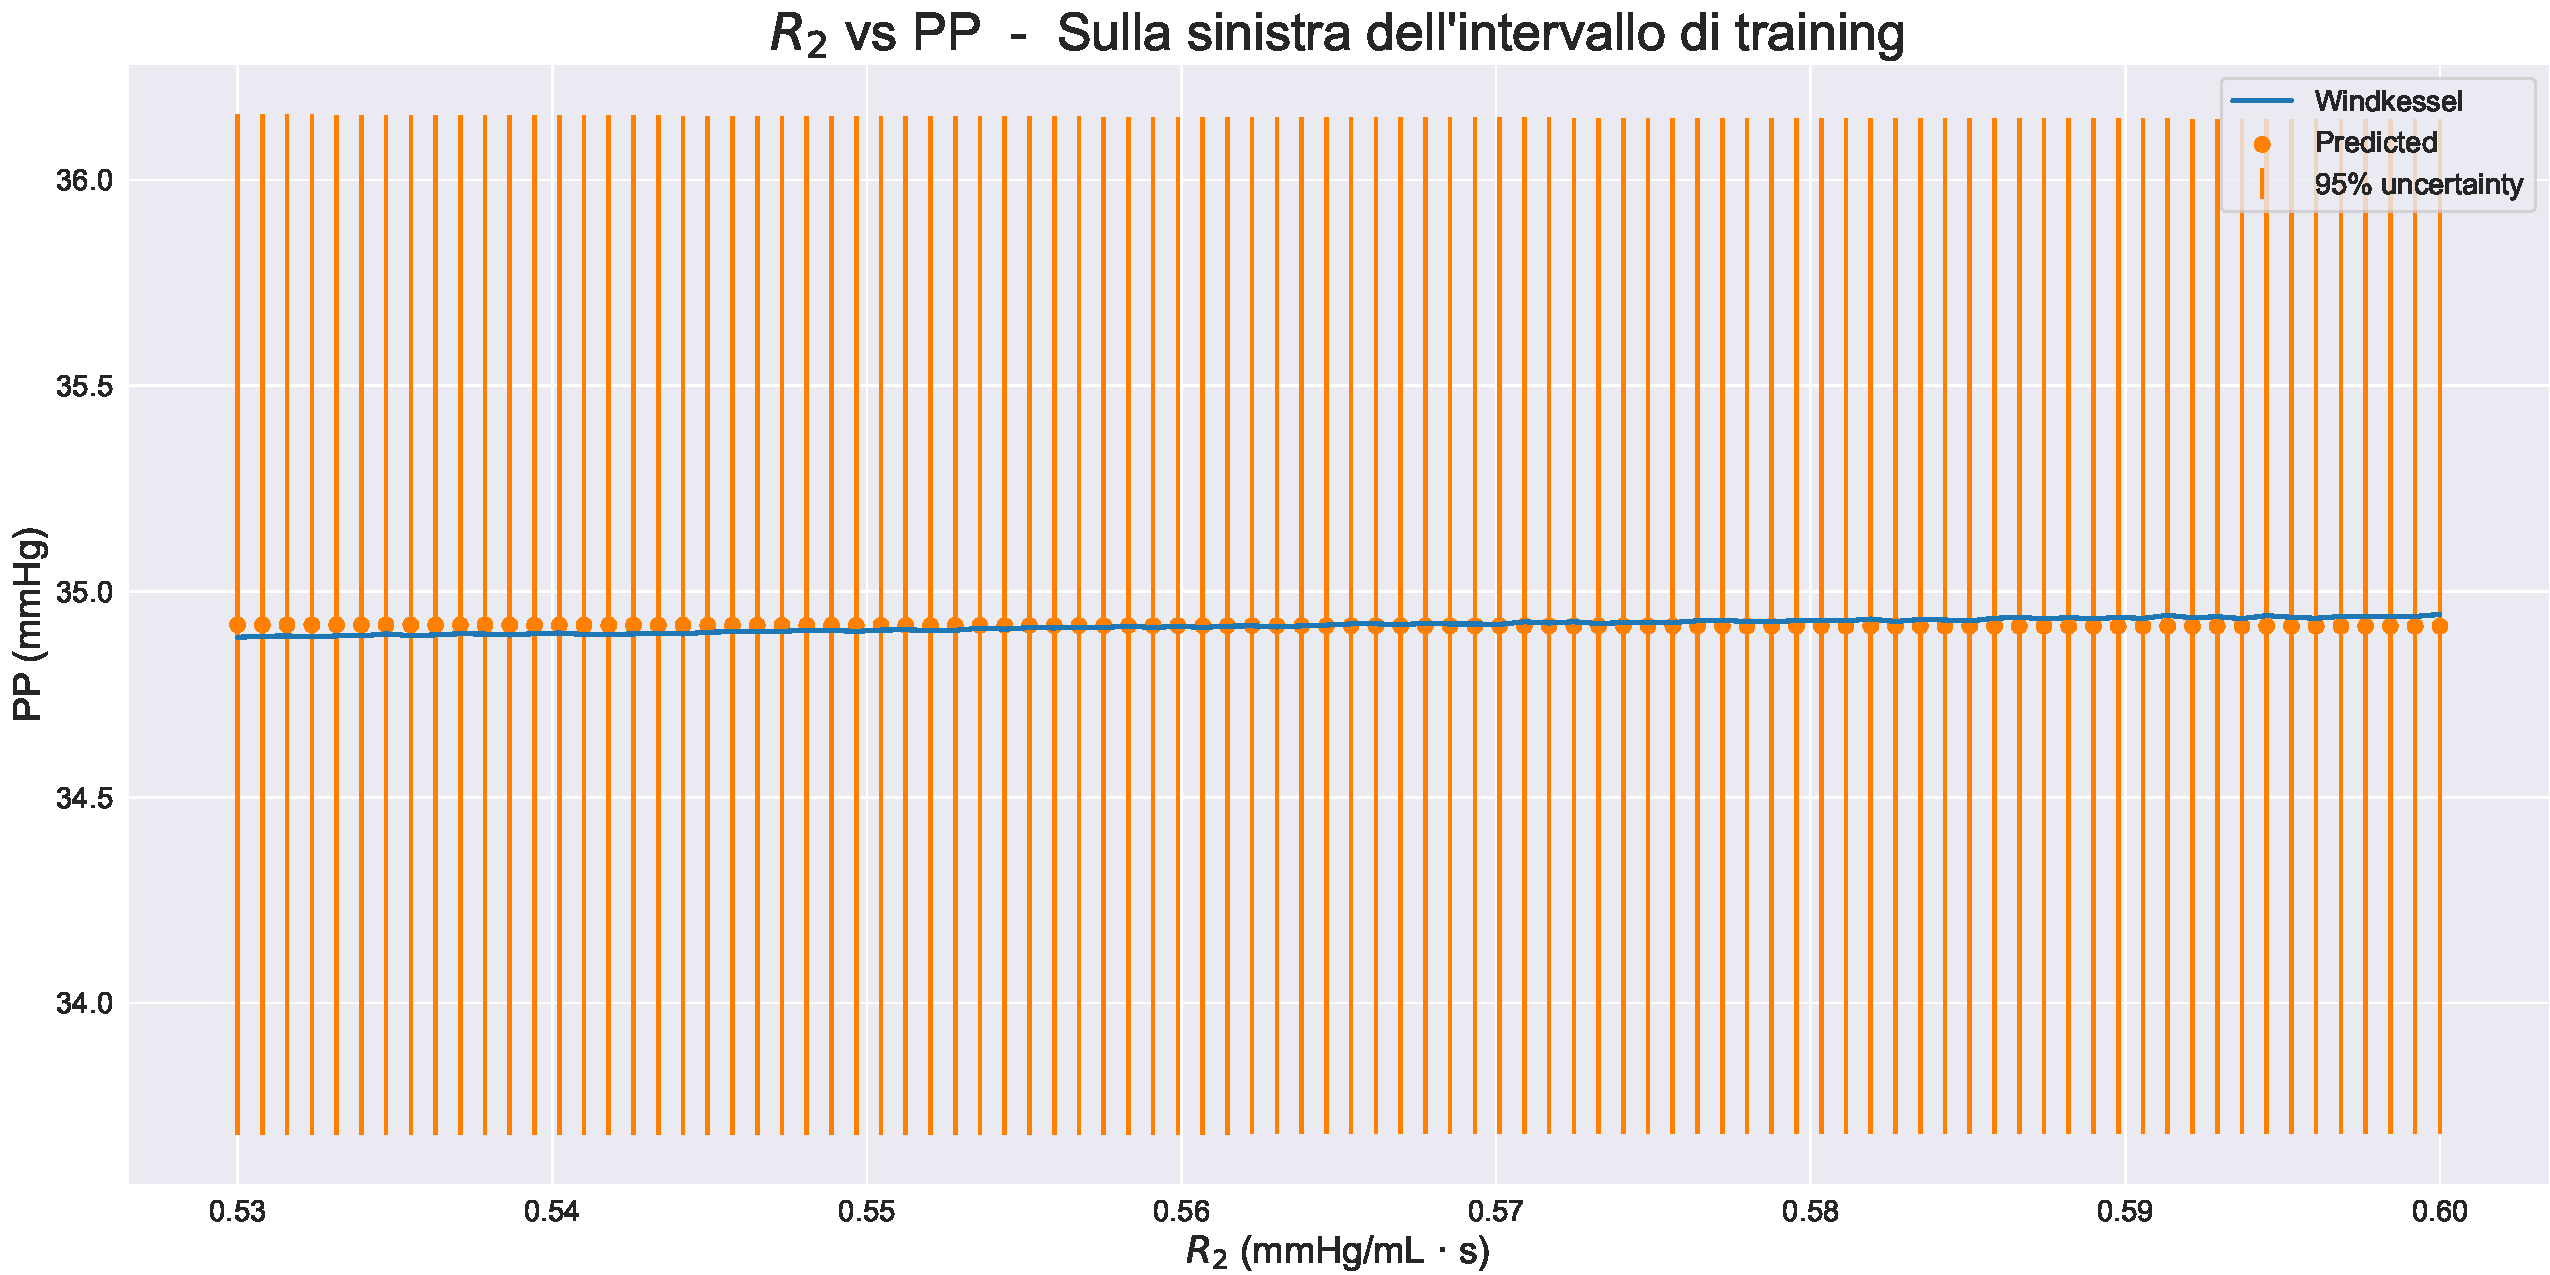
\includegraphics[width=1\textwidth]{images/Training (risultati)/PP/PP - R2 - sx.pdf}
    \caption{Dependence of PP on $R2$ on the adjacent interval to the left of the training interval.}
    \label{PP - R2 - sx}
\end{figure}



\begin{figure}
    \centering
    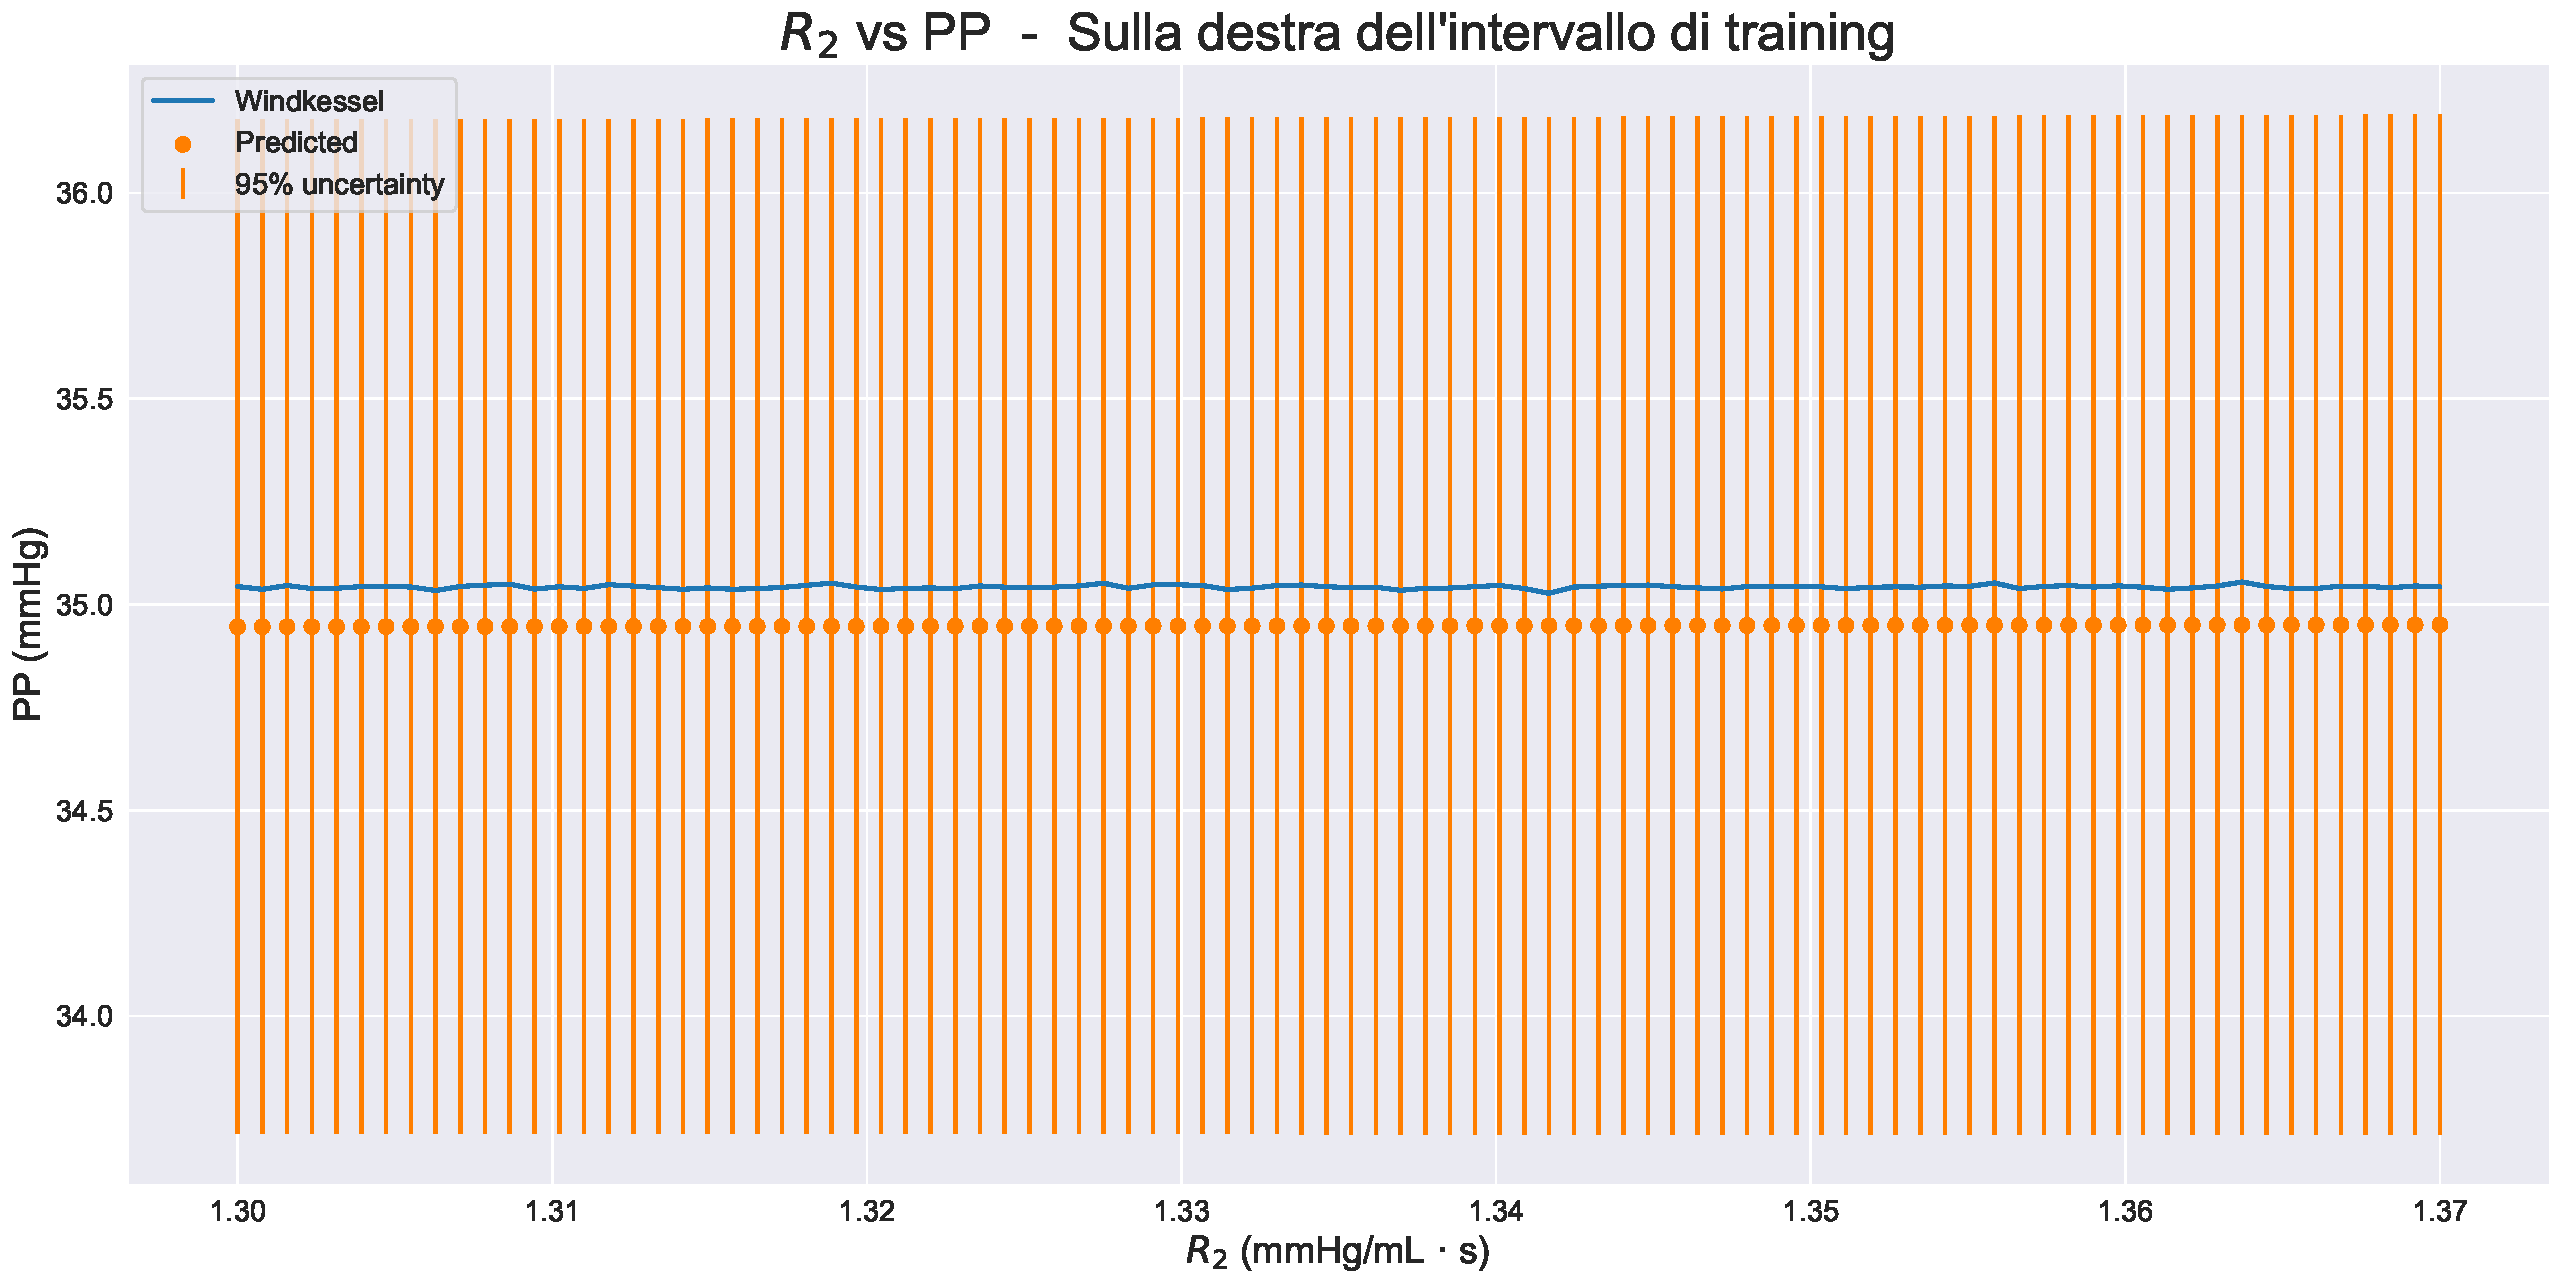
\includegraphics[width=1\textwidth]{images/Training (risultati)/PP/PP - R2 - dx.pdf}
    \caption{Dependence of PP on $R2$ on the adjoint interval to the right of the training interval.}
    \label{PP - R2 - dx}
\end{figure}







\newpage

%******************************
%*********** SBP **************
%******************************
\subsection{Systolic blood pressure (SBP)}
$\text{lr}=0.07$ is imposed and the early stopper \textit{GLEarlyStoppingCriterion} is used with parameters: $\alpha = 5$, $\text{patience}=1$.

% **********
% SBP - loss
% **********
\subsubsection{Training and validation loss}
The training needed one hundred and thirteen EPOCHS, concluded with $\text{R2Score}=0.9999$, $\text{MeanSquaredError}=0.0052$. Figure \ref{SBP - loss} shows the training and validation loss trend with MSE and R2Score; in green is the early stopper trend.
\begin{figure}[h]
    \centering
    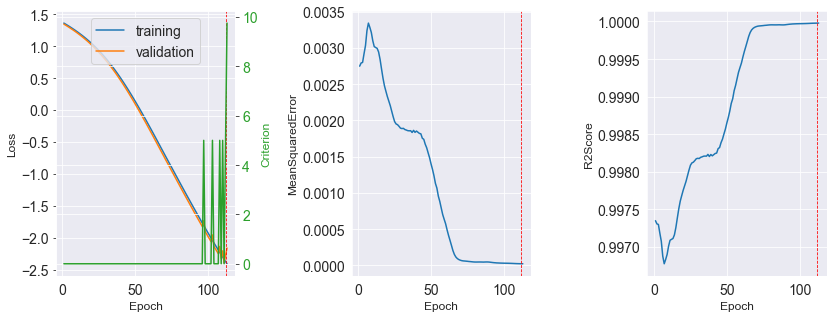
\includegraphics[width=1\textwidth]{images/Training (risultati)/SBP/SBP - loss.png}
    \caption{SBP: andamento del training e validation loss, early stopper, R2Score e MSE.}
    \label{SBP - loss}
\end{figure}

\vspace{-0.5cm}

% **********
% SBP - inference
% **********
\subsubsection{Approximation of input data}
Figure \ref{SBP - inference} shows how the predictions approximate the input data. The error bars are $0.0012$ long, so they are not noticeable.

\begin{figure}[h]
    \centering
    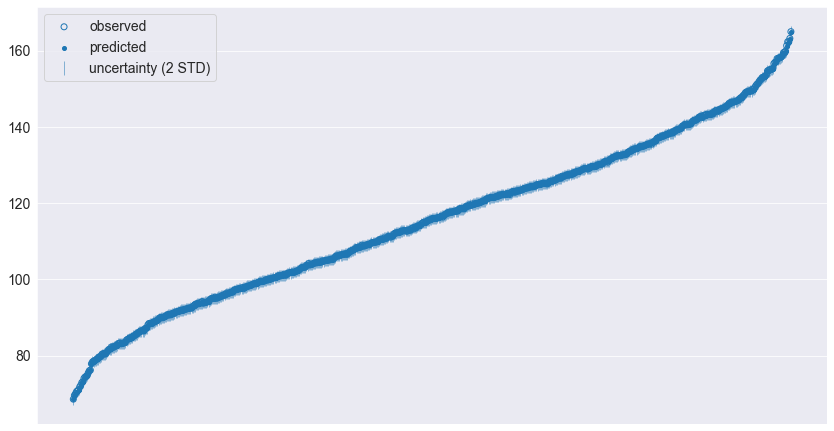
\includegraphics[width=1\textwidth]{images/Training (risultati)/SBP/SBP - inference.png}
    \caption{SBP: predictions about the input data.}
    \label{SBP - inference}
\end{figure}



% **********
% SBP - C
% **********
\subsubsection{Dependence on $C$}
The overall result is shown in figure \ref{SBP - C - full}, the result in the training interval alone in \ref{SBP - C - training}, the result in the individual adjacent intervals in \ref{SBP - C - sx} and \ref{SBP - C - dx}.

\vspace{1cm}

\begin{figure}[!htb]
    \centering
    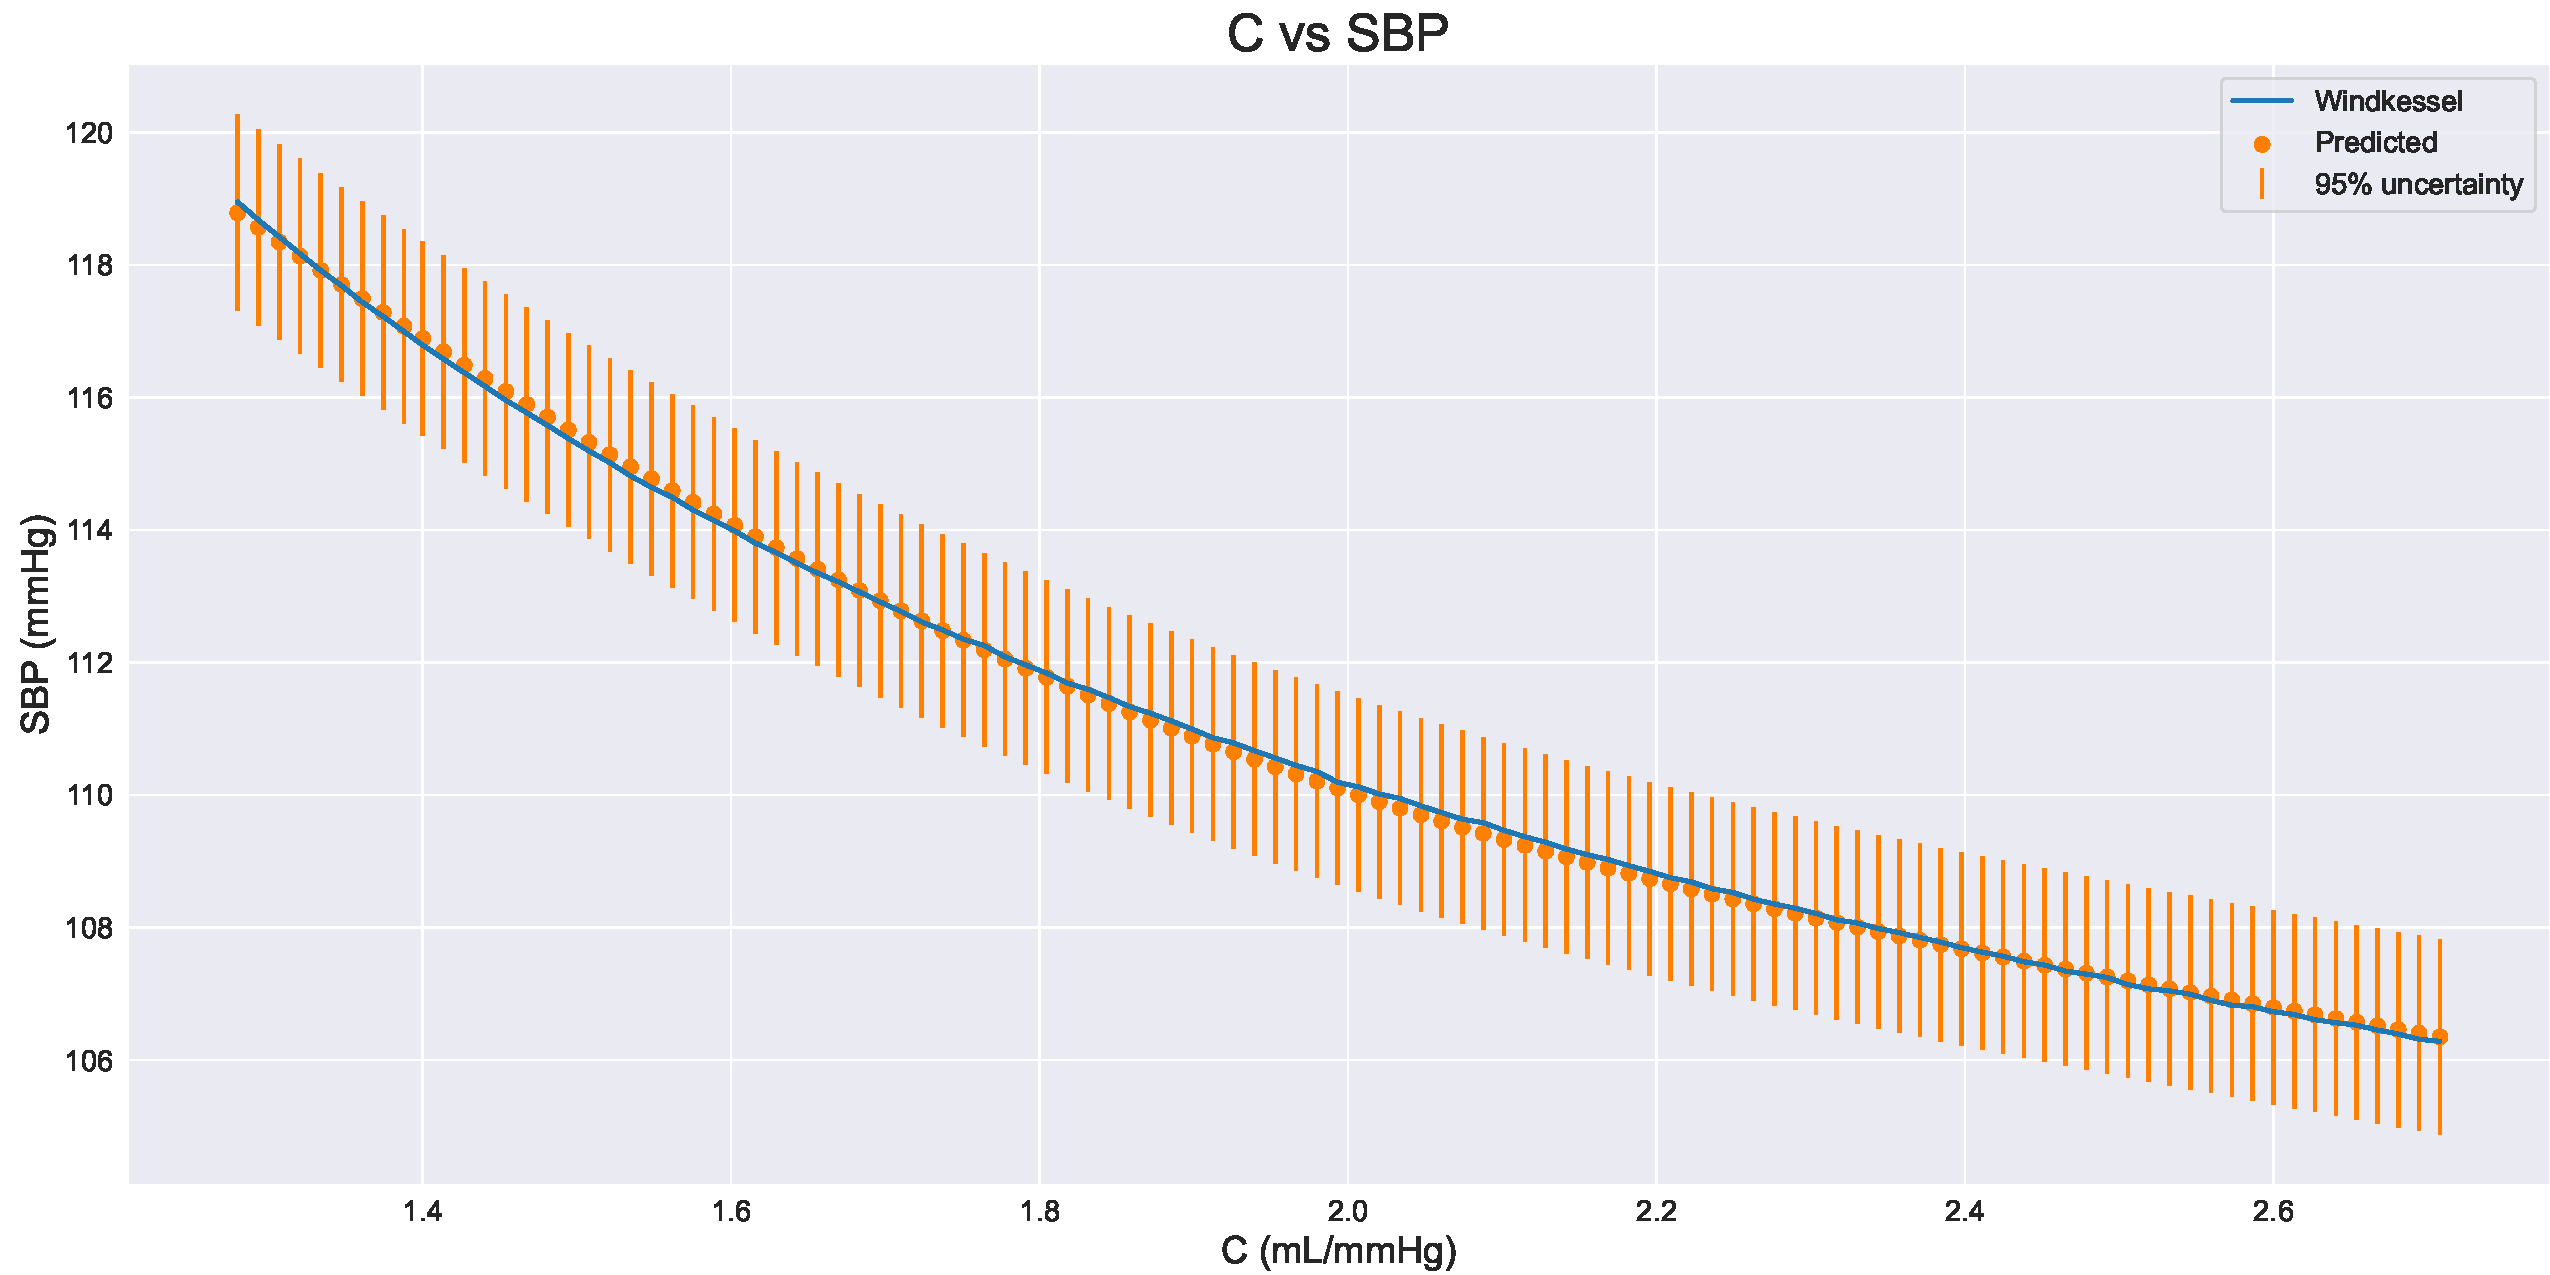
\includegraphics[width=1\textwidth]{images/Training (risultati)/SBP/SBP - C - full.pdf}
    \caption{Dependence of SBP on $C$ on the training interval and two adjacent intervals.}
    \label{SBP - C - full}
\end{figure}

\vspace{0.32cm}

\begin{figure}[!htb]
    \centering
    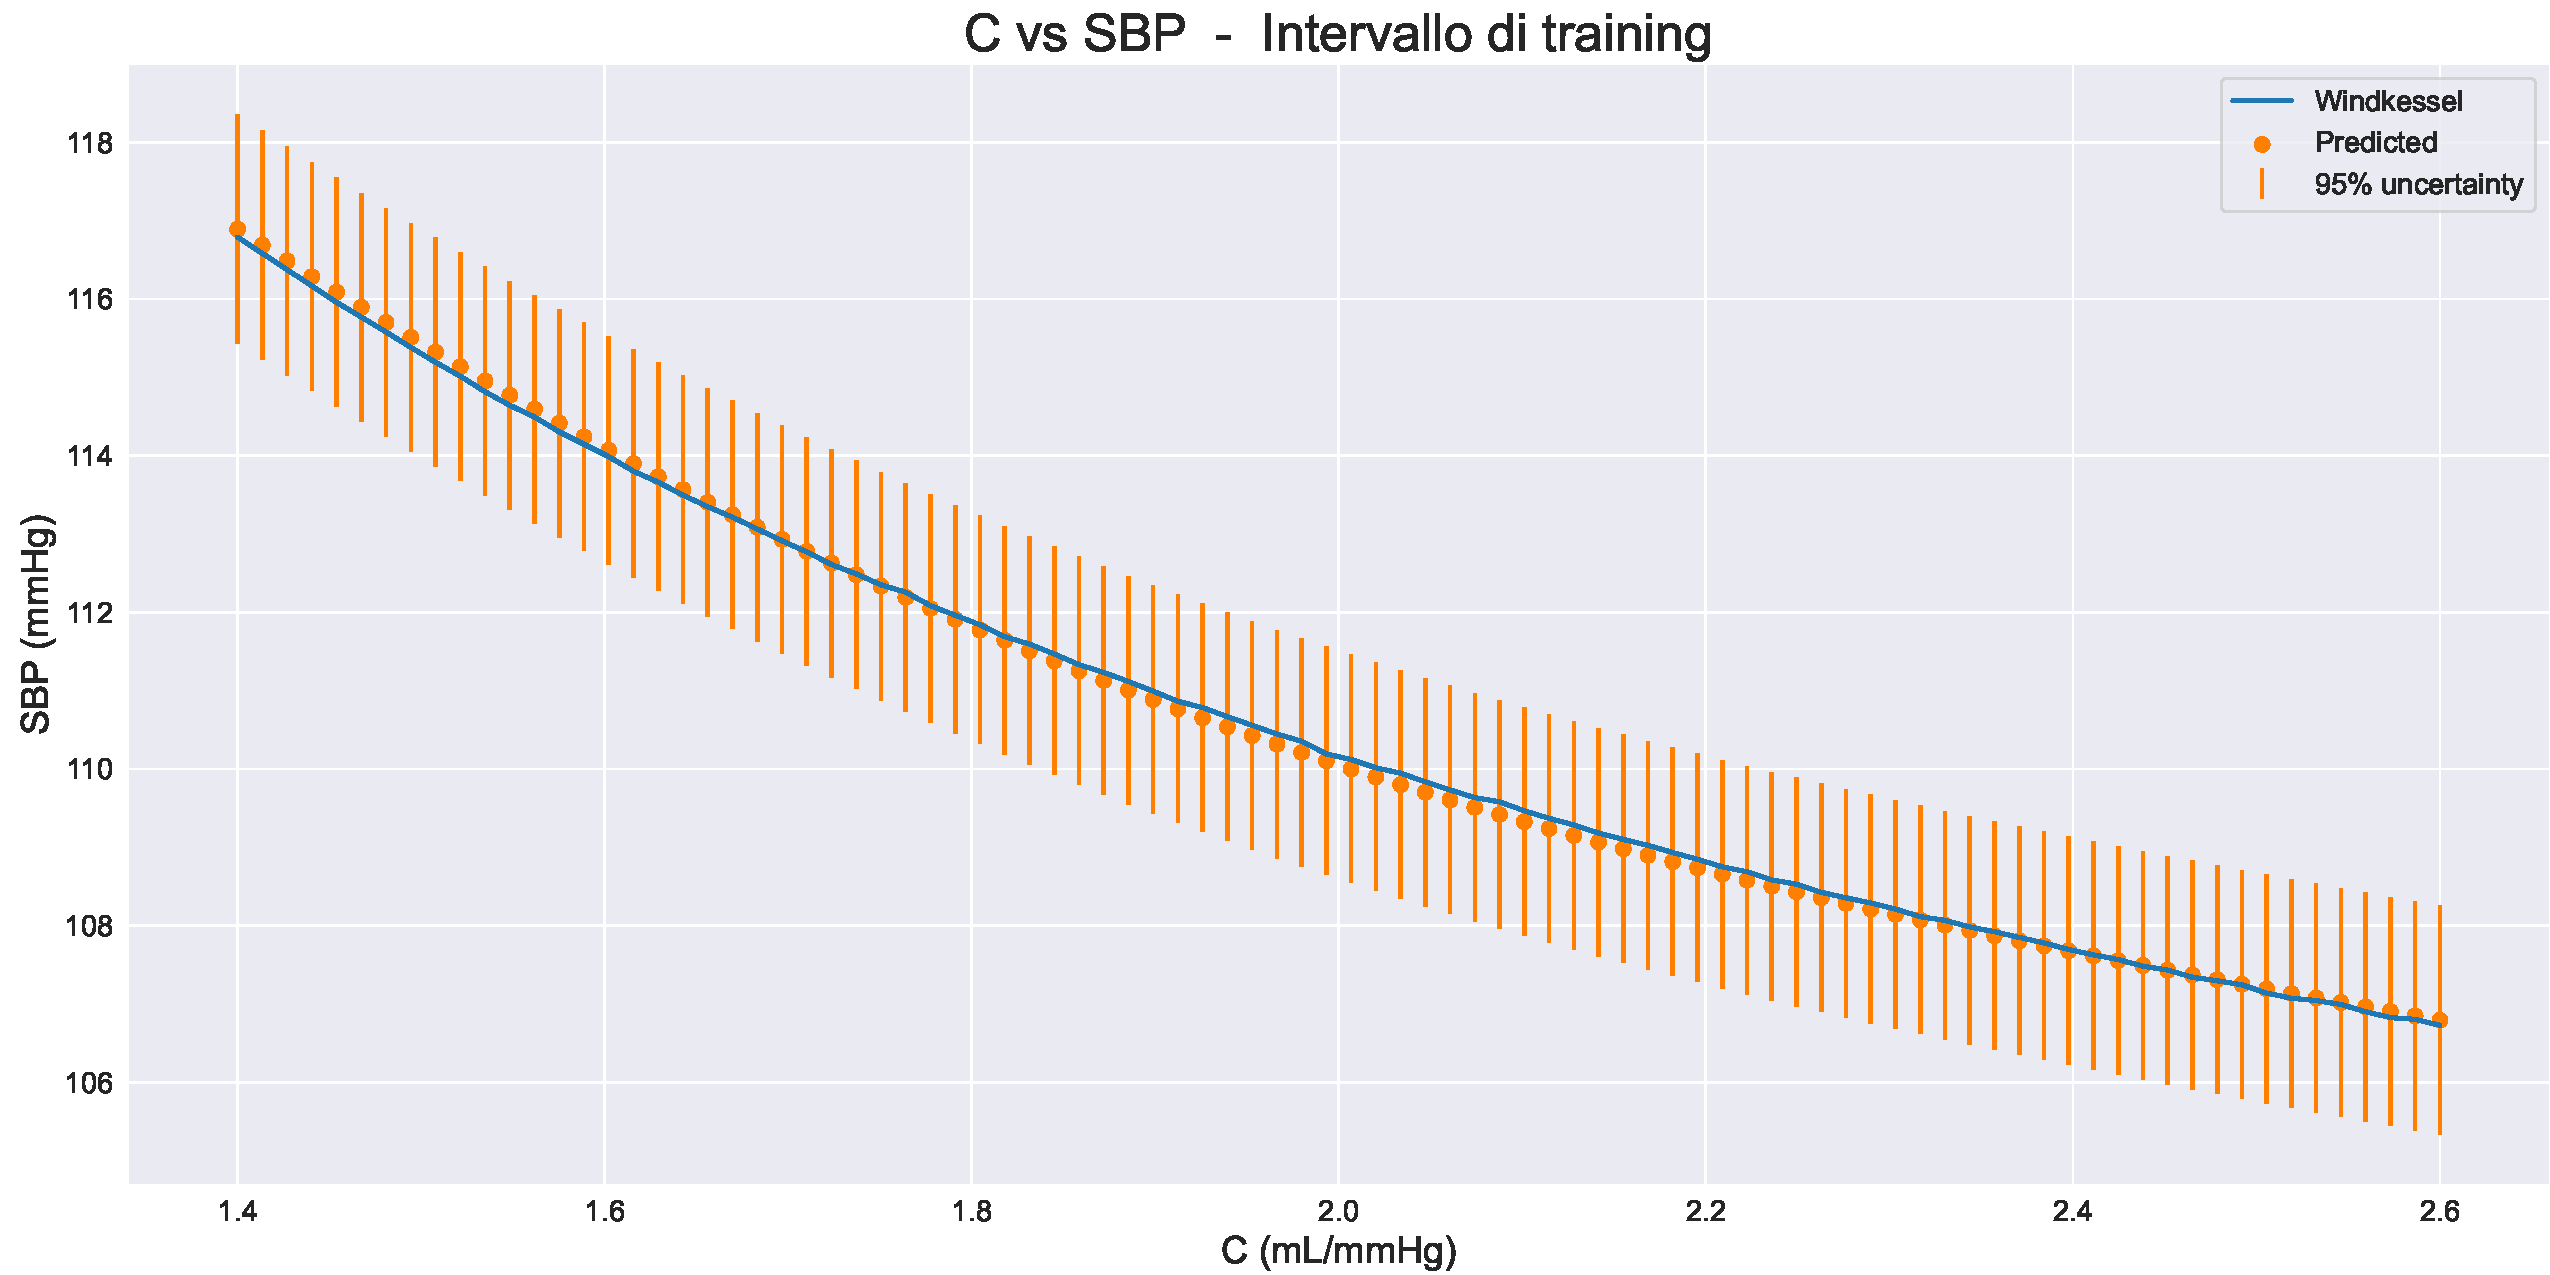
\includegraphics[width=1\textwidth]{images/Training (risultati)/SBP/SBP - C - training.pdf}
    \caption{Dependence of SBP on $C$ over the training interval.}
    \label{SBP - C - training}
\end{figure}

\begin{figure}
    \centering
    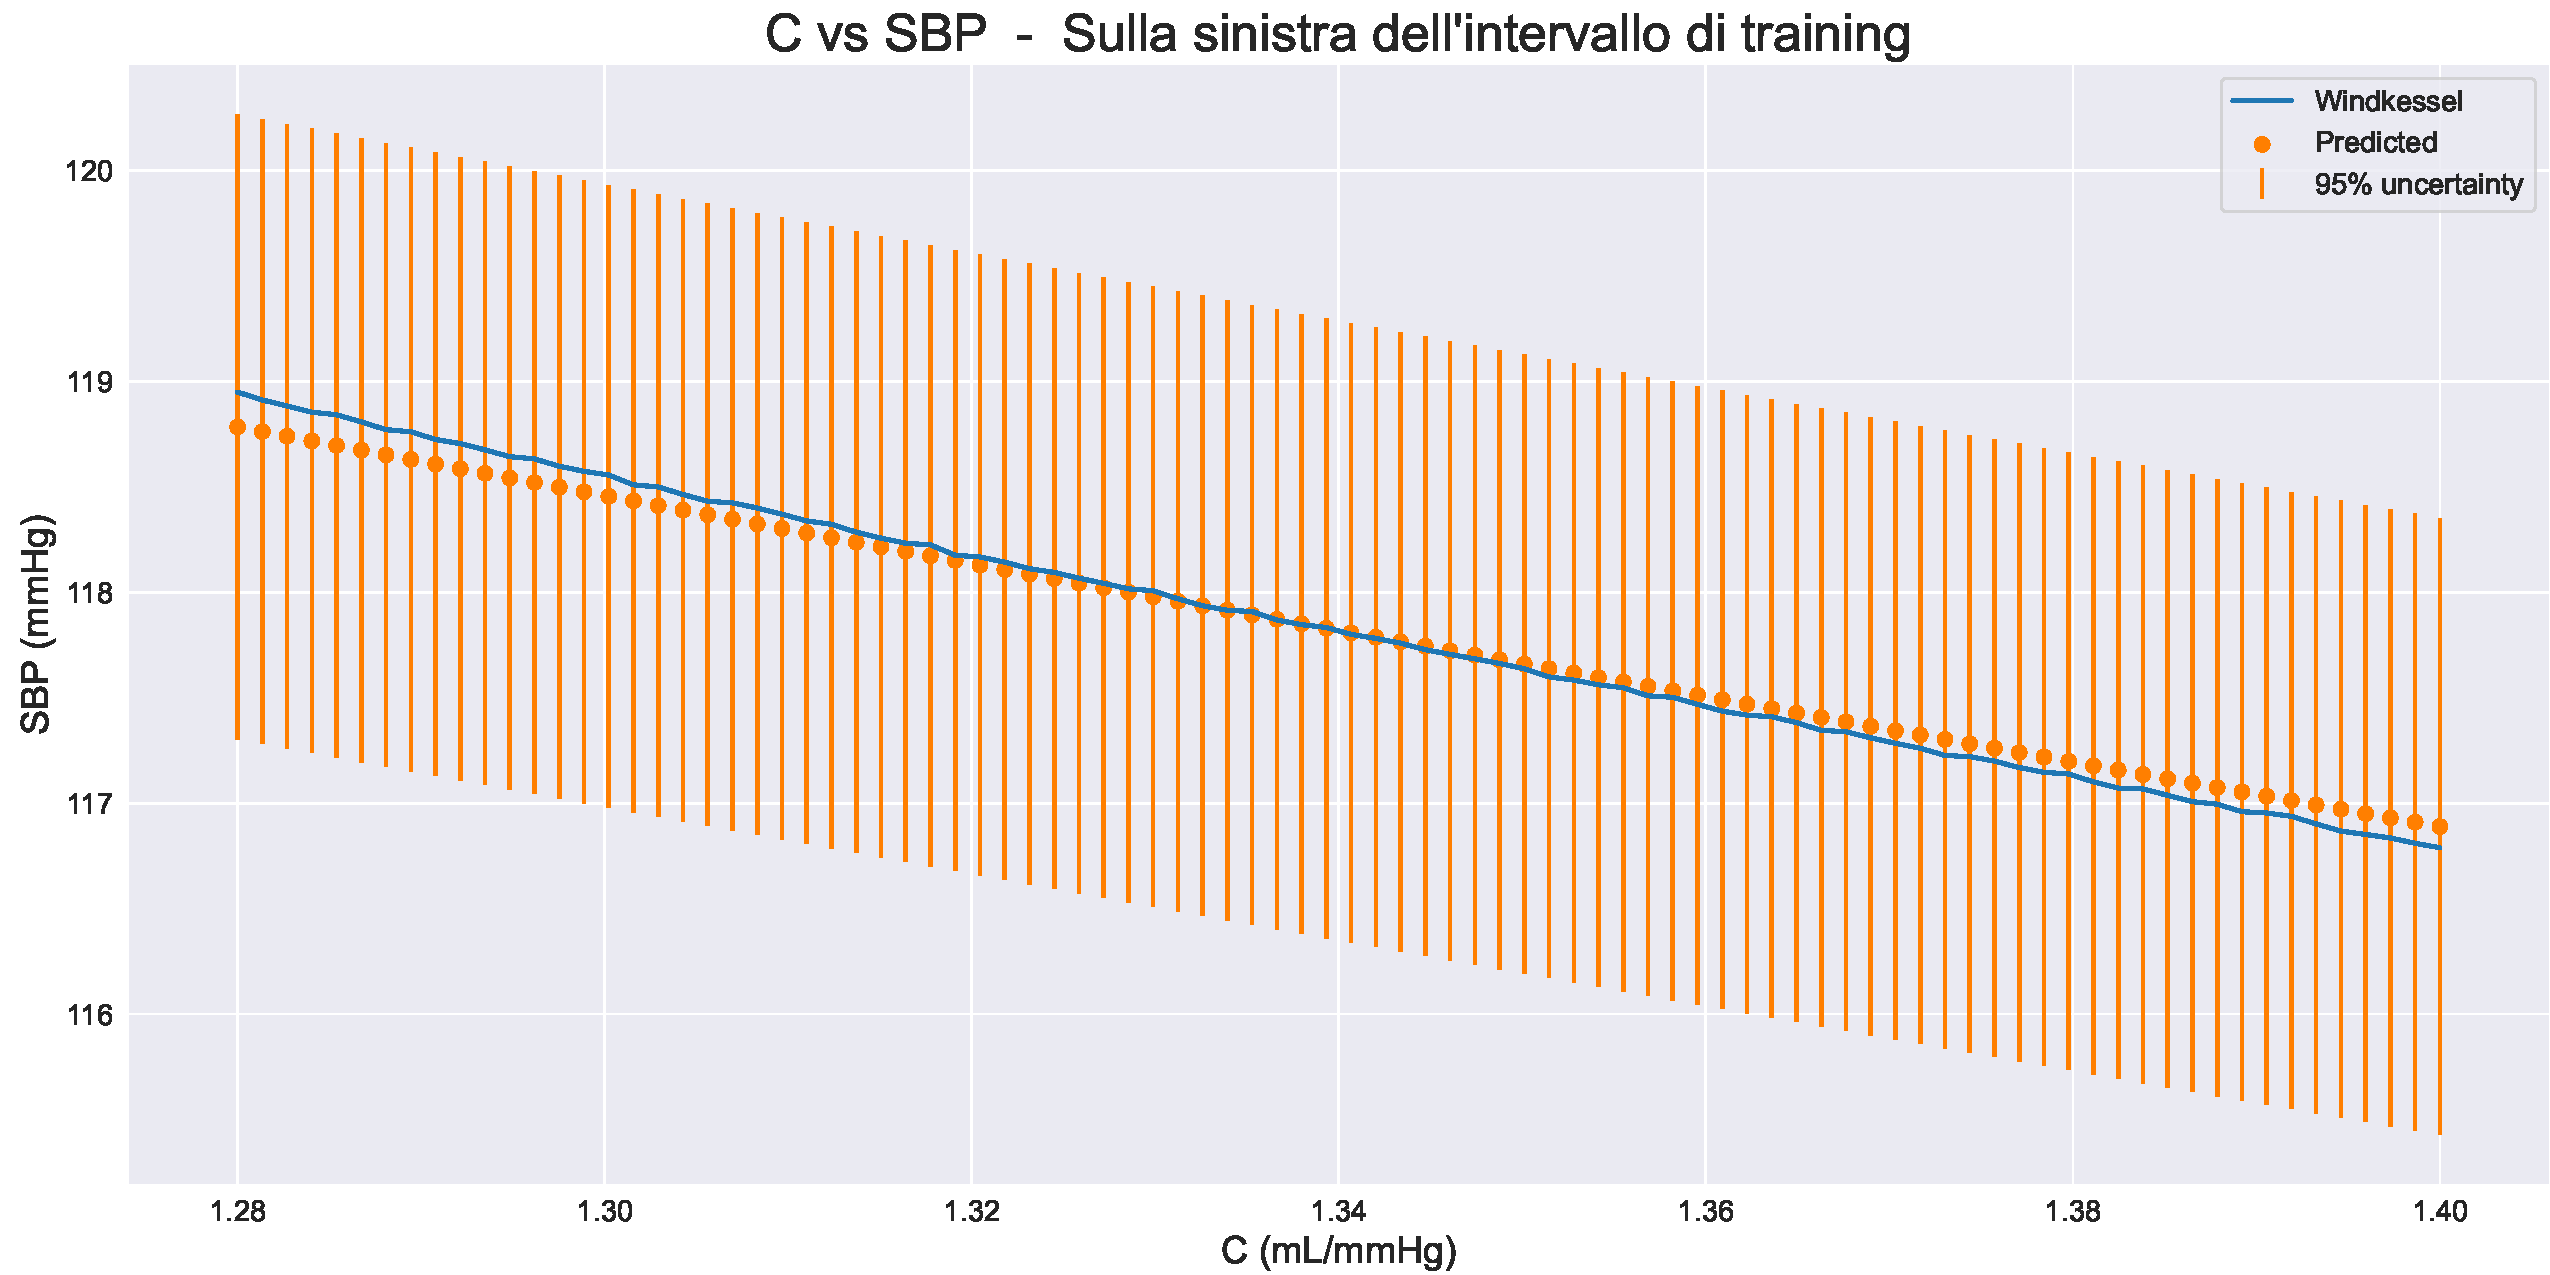
\includegraphics[width=1\textwidth]{images/Training (risultati)/SBP/SBP - C - sx.pdf}
    \caption{Dependence of SBP on $C$ on the adjacent interval to the left of the training interval.}
    \label{SBP - C - sx}
\end{figure}


\begin{figure}
    \centering
    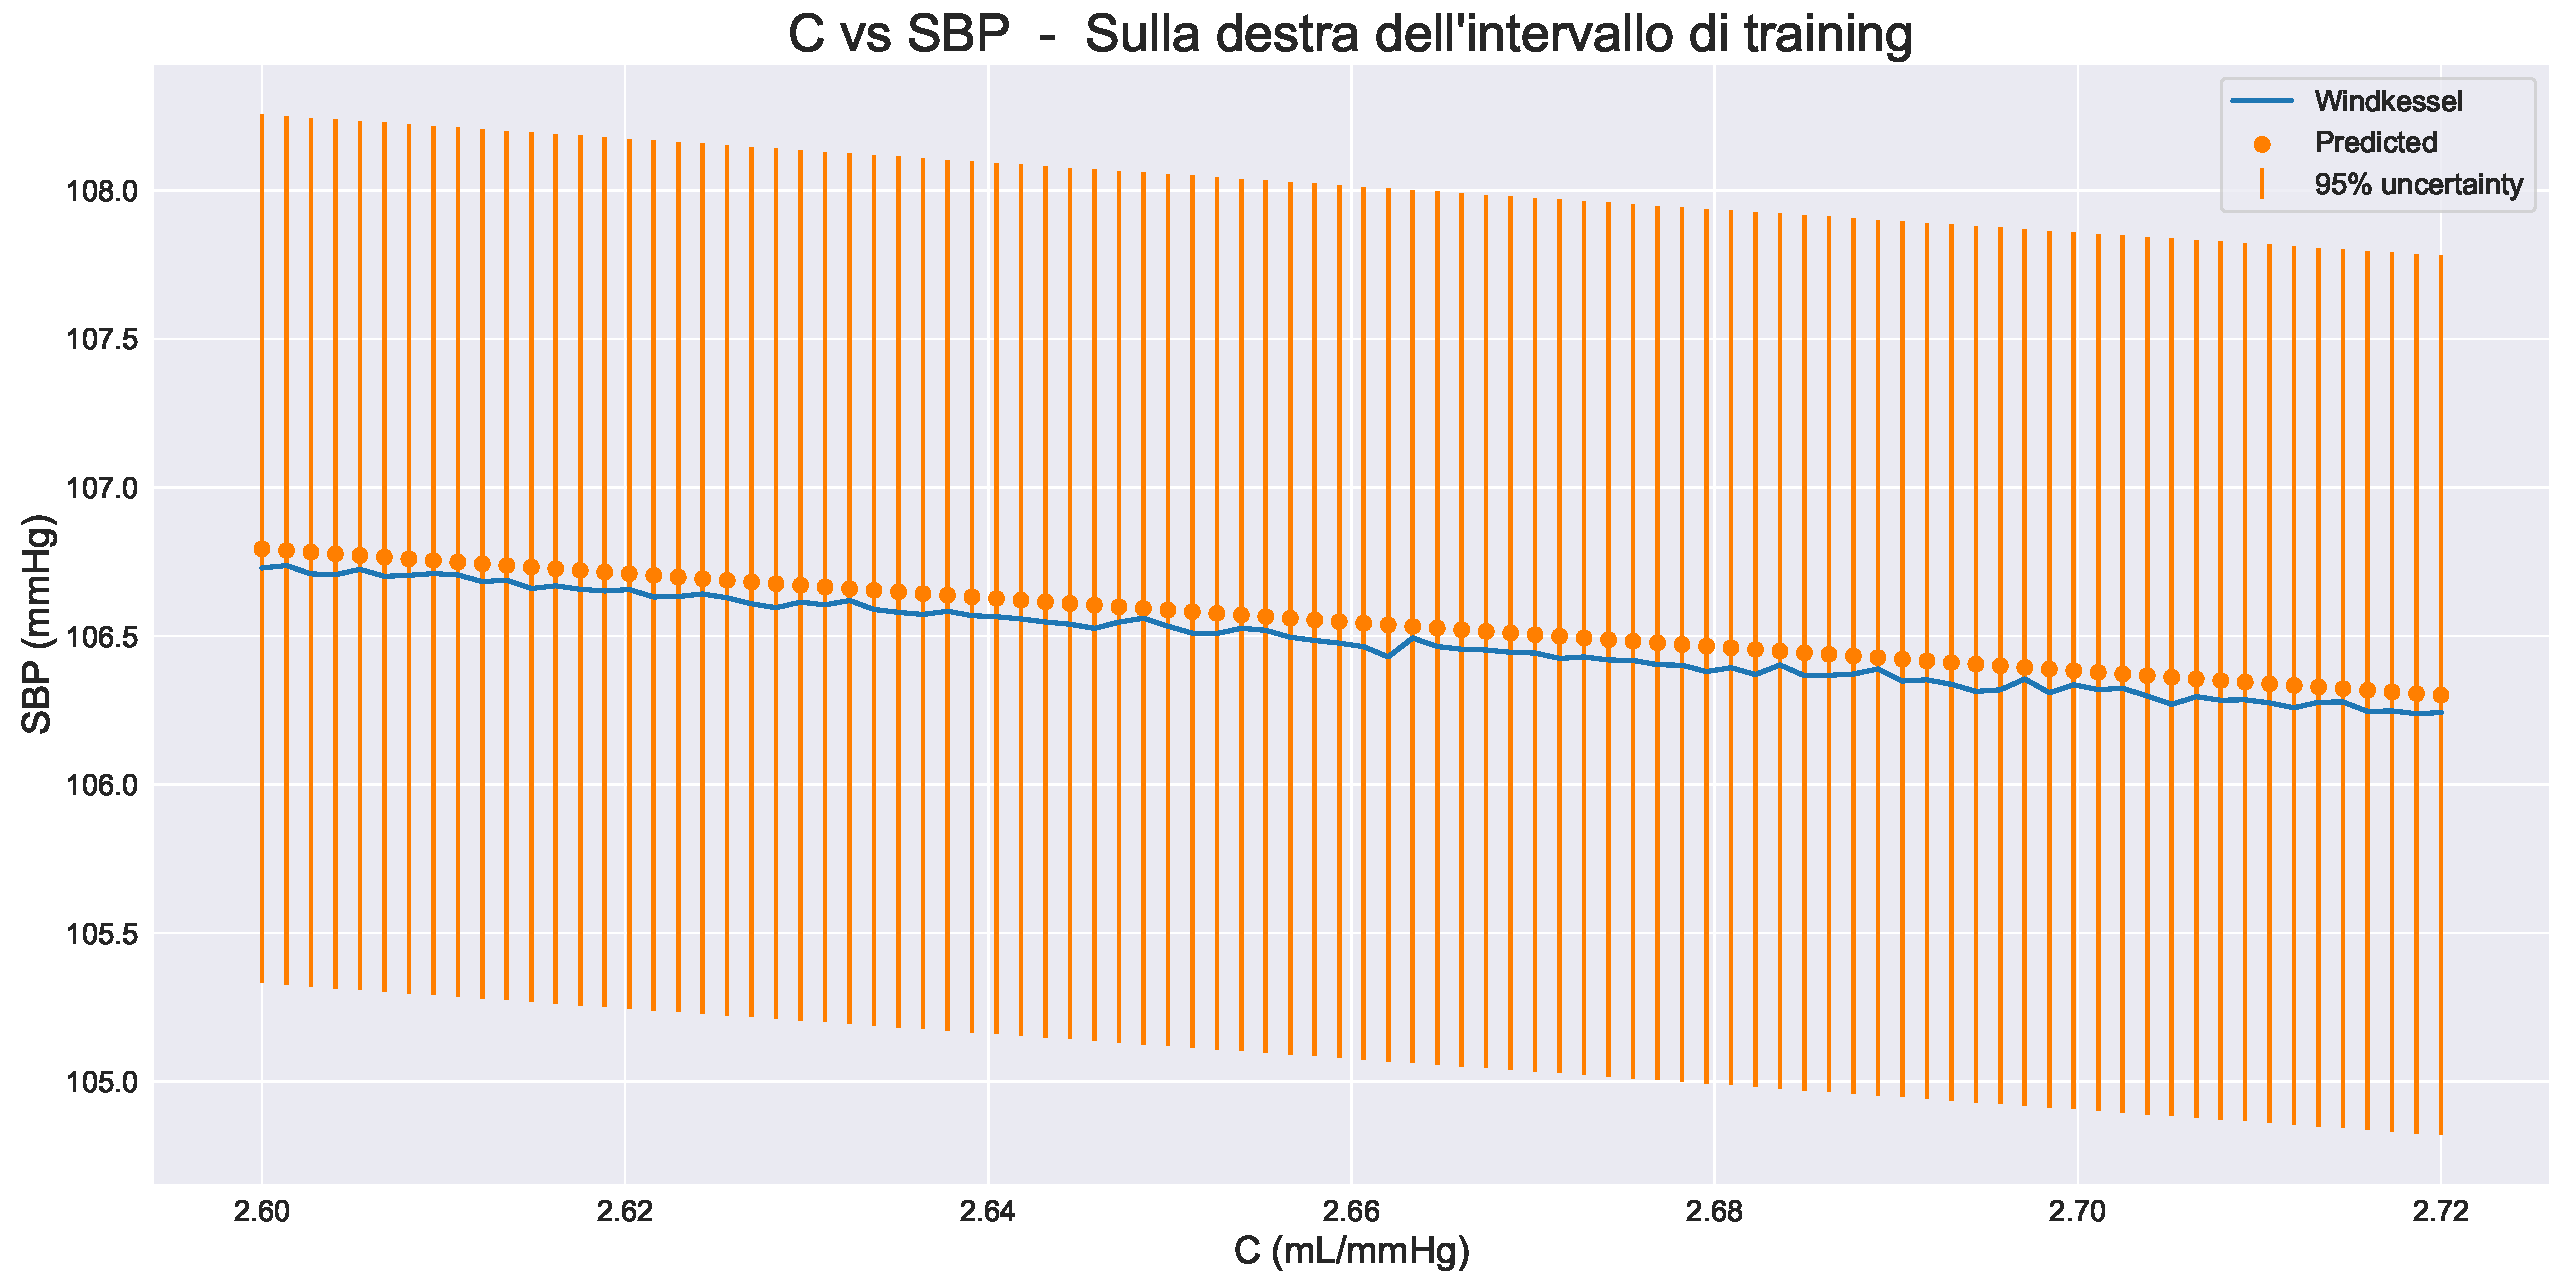
\includegraphics[width=1\textwidth]{images/Training (risultati)/SBP/SBP - C - dx.pdf}
    \caption{Dependence of SBP on $C$ on the adjacent interval to the right of the training interval.}
    \label{SBP - C - dx}
\end{figure}



\newpage

% **********
% SBP - R1
% **********
\subsubsection{Dependence on $R_1$}
The overall result is shown in figure \ref{SBP - R1 - full}, the result in the training interval alone in \ref{SBP - R1 - training}, the result in the individual adjacent intervals in \ref{SBP - R1 - sx} and \ref{SBP - R1 - dx}.

\vspace{0.7cm}


\begin{figure}[!htb]
    \centering
    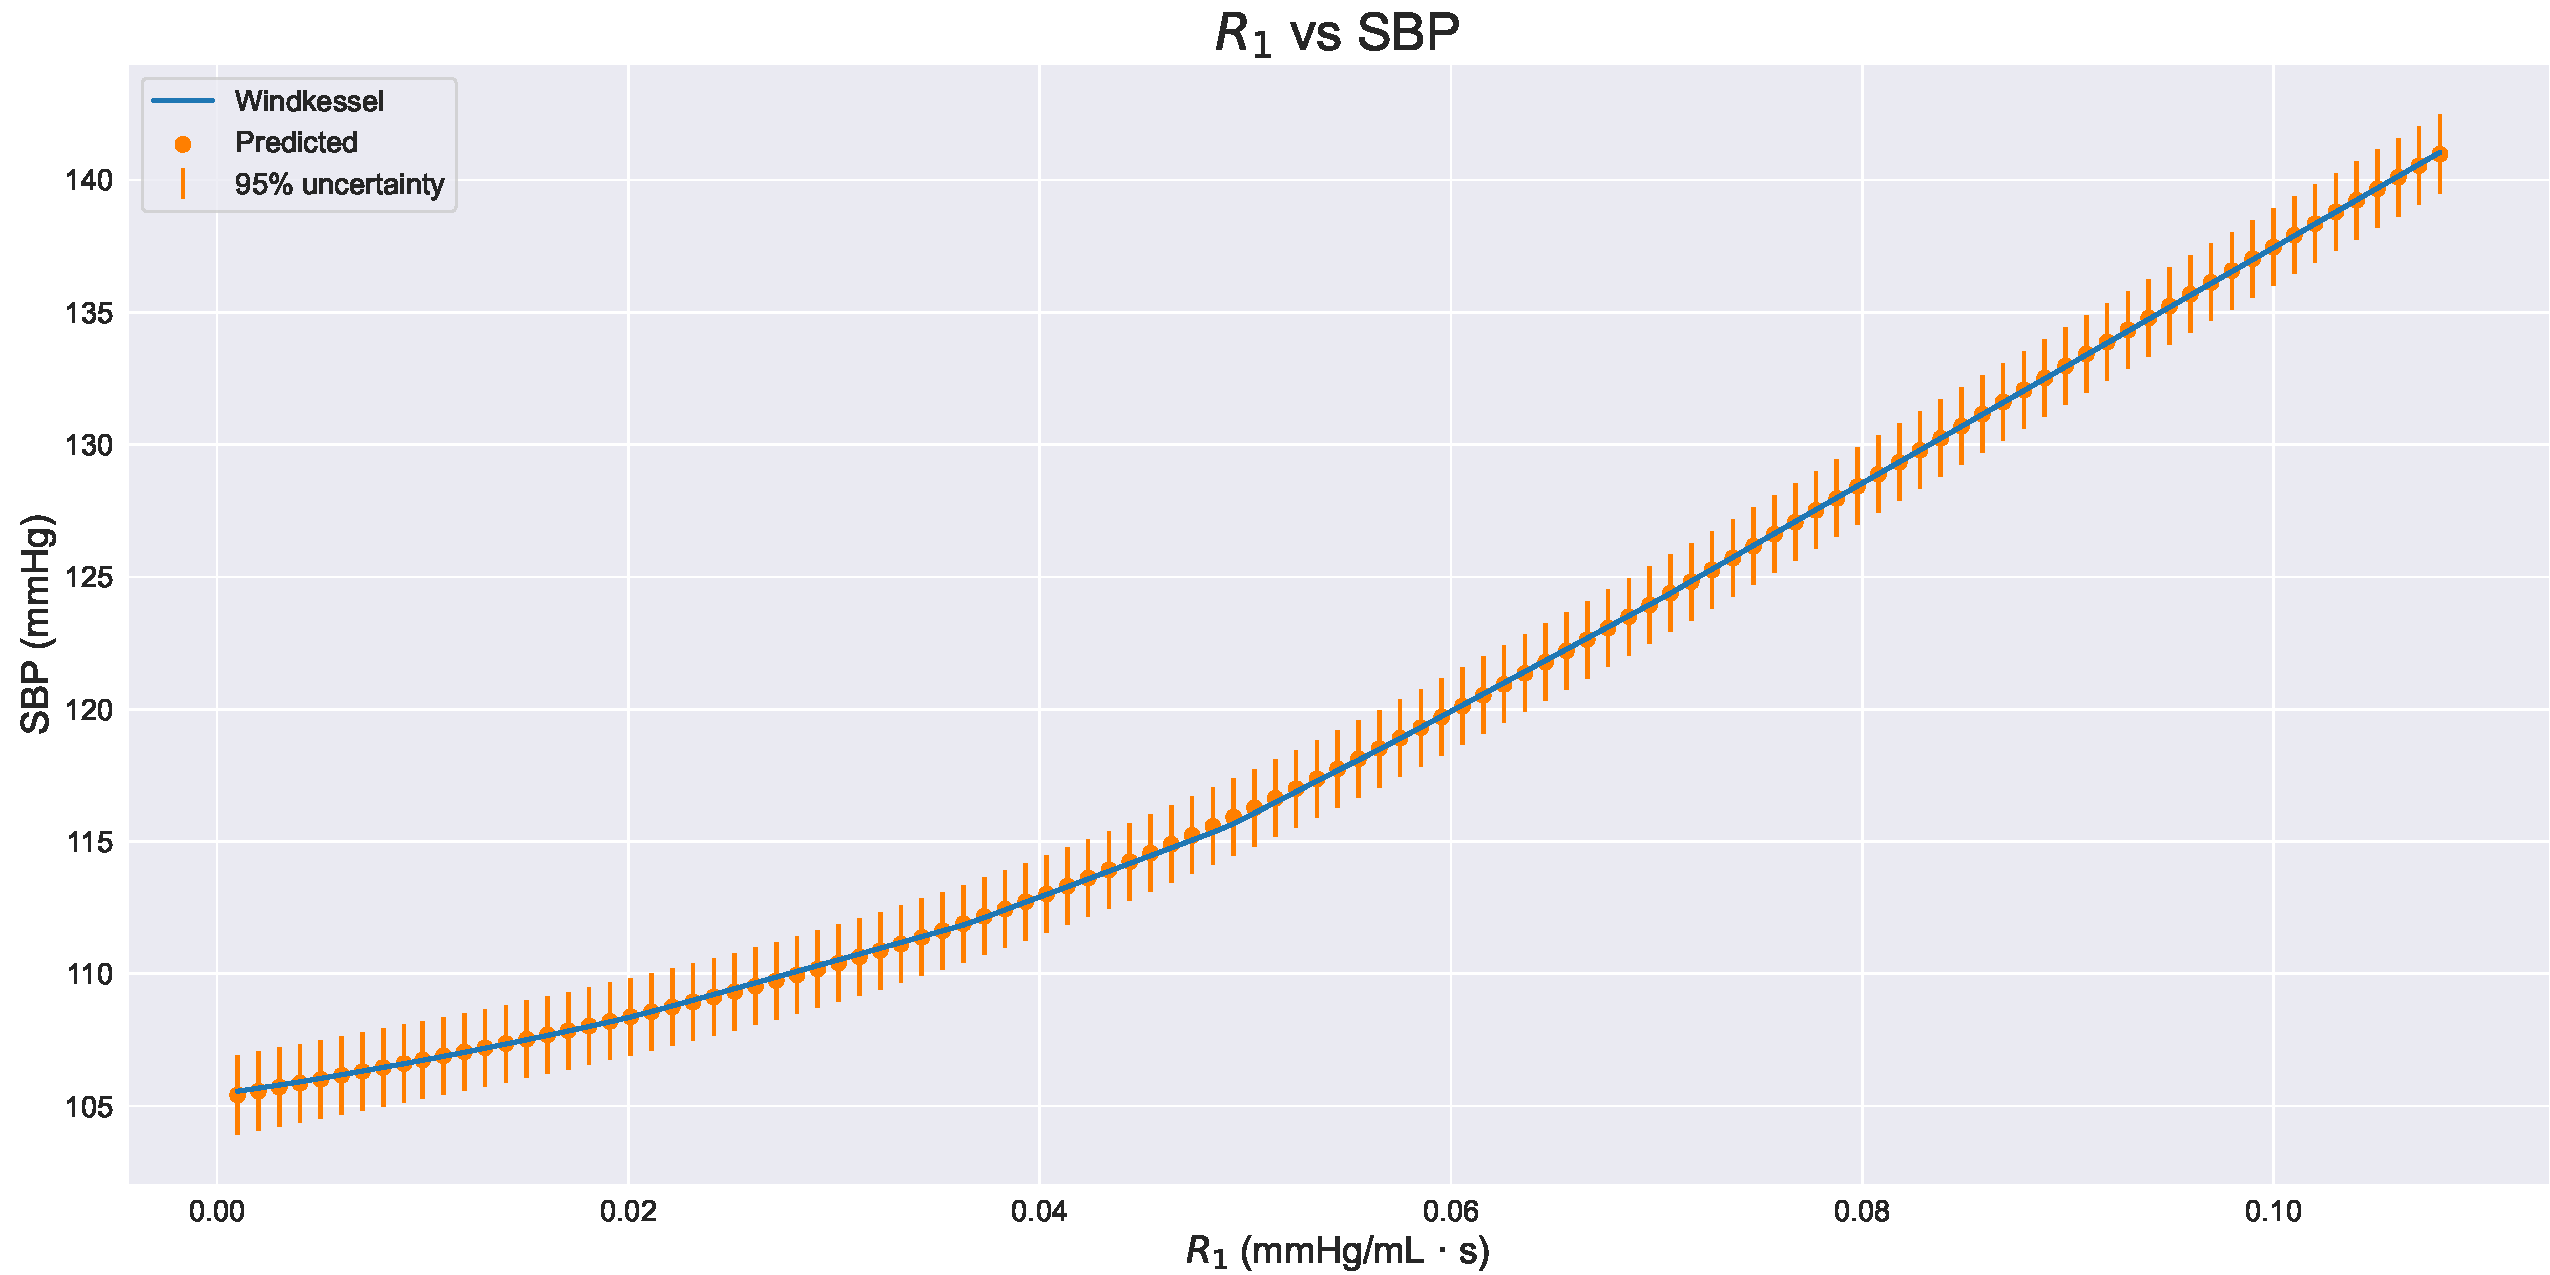
\includegraphics[width=1\textwidth]{images/Training (risultati)/SBP/SBP - R1 - full.pdf}
    \caption{Dependence of SBP on $R1$ on the training interval and two adjacent intervals.}
    \label{SBP - R1 - full}
\end{figure}

\vspace{0.32cm}

\begin{figure}[!htb]
    \centering
    \includegraphics[width=1\textwidth]{images/Training (risultati)/SBP/SBP - R1 - training.pdf}
    \caption{Dependence of SBP on $R1$ over the training interval.}
    \label{SBP - R1 - training}
\end{figure}

\begin{figure}
    \centering
    \includegraphics[width=1\textwidth]{images/Training (risultati)/SBP/SBP - R1 - sx.pdf}
    \caption{Dependence of SBP on $R1$ on the adjacent interval to the left of the training interval.}
    \label{SBP - R1 - sx}
\end{figure}



\begin{figure}
    \centering
    \includegraphics[width=1\textwidth]{images/Training (risultati)/SBP/SBP - R1 - dx.pdf}
    \caption{Dependence of SBP on $R1$ on the adjacent interval to the right of the training interval.}
    \label{SBP - R1 - dx}
\end{figure}






\newpage
% **********
% SBP - R2
% **********
\subsubsection{Dependence on $R_2$}
The overall result is shown in figure \ref{SBP - R2 - full}, the result in the training interval alone in \ref{SBP - R2 - training}, the result in the individual adjacent intervals in \ref{SBP - R2 - sx} and \ref{SBP - R2 - dx}.

\vspace{1cm}

\begin{figure}[!htb]
    \centering
    \includegraphics[width=1\textwidth]{images/Training (risultati)/SBP/SBP - R2 - full.pdf}
    \caption{Dependence of SBP on $R2$ on the training interval and two adjacent intervals.}
    \label{SBP - R2 - full}
\end{figure}

\vspace{0.32cm}

\begin{figure}[!htb]
    \centering
    \includegraphics[width=1\textwidth]{images/Training (risultati)/SBP/SBP - R2 - training.pdf}
    \caption{Dependence of SBP on $R2$ over the training interval.}
    \label{SBP - R2 - training}
\end{figure}

\begin{figure}
    \centering
    \includegraphics[width=1\textwidth]{images/Training (risultati)/SBP/SBP - R2 - sx.pdf}
    \caption{Dependence of SBP on $R2$ on the adjacent interval to the left of the training interval.}
    \label{SBP - R2 - sx}
\end{figure}



\begin{figure}
    \centering
    \includegraphics[width=1\textwidth]{images/Training (risultati)/SBP/SBP - R2 - dx.pdf}
    \caption{Dependence of SBP on $R2$ on the adjacent interval to the right of the training interval.}
    \label{SBP - R2 - dx}
\end{figure}

\section{Running time: approximation of MAP, DBP, SBP, PP}
As done in \ref{Windkessel: tempo esecuzione}, we now calculate the run time to find the value of MAP, DBP, SBP, PP from the values of $C, R_1, R_2$. Since one training is performed for each parameter, the parameter estimation times for each trained model are reported.

% Please add the following required packages to your document preamble:
% \usepackage{lscape}

\begin{table}[!htb]
\centering
\begin{tabular}{cc}
\hline
\textbf{Parametro stimato} & \textbf{\begin{tabular}[c]{@{}c@{}}Tempo esecuzione\\ (media + dev. std.)\end{tabular}} \\ \hline
DBP & 5.89 ms ± 1.63 ms \\
SBP & 5.23 ms ± 1.75 ms \\
MAP & 5.6 ms ± 1.64 ms  \\
PP  & 4.03 ms ± 1.19 ms \\ \hline
\end{tabular}
\caption{Tempo di esecuzione per trovare l’approssimazione dei parametri usando i processi gaussiani addestrati.}
\label{tab: tempo par}
\end{table}


Since an independent model is trained for each parameter, it is necessary to run the four trained Gaussian processes to obtain the MAP, DBP, SBP and PP values. So the running time needed to obtain the approximations of the four parameters is the sum of the times needed to obtain them one by one. So it can be said that in all, an average of 20.75 ms is required to obtain the four values.
Comparing this quantity to the table \ref{tab: tempo windkessel} it is evident that using Gaussian processes takes much less time than approximating the solution of the Windkessel model already after only ten cardiac cycles (a rather low number if the goal is to find the solution at convergence). \\


Evidently, then, Gaussian processes solve the run-time problem in the Windkessel model by providing a good approximation of the value of MAP, DBP, SBP, PP.
